\documentclass[12pt, a4paper]{book}

\usepackage[utf8]{inputenc}
\usepackage[spanish]{babel}
\usepackage{geometry}
\usepackage[square,numbers,sectionbib]{natbib}
\usepackage{chapterbib}
\usepackage{graphicx}
\usepackage{tabularx}
\usepackage{subfig}
\usepackage[version=3]{mhchem}  %for chemistry
\usepackage{xcolor}
\usepackage{wrapfig}
\usepackage[font=small,labelfont=bf]{caption}
\usepackage{amssymb}		
\usepackage{longtable}
\usepackage{epsfig}
\usepackage{colortbl}
%\usepackage{picins}
%\usepackage[usenames]{color}

  

%\usepackage{amsmath}
\usepackage{bm}
\usepackage{fancyhdr}
  
\newcommand{\br}{\mathbf{r}}
\newcommand{\bR}{\mathbf{R}}
\newcommand{\ham}{\mathcal{H}}
\newcommand{\bra}[1]{\langle#1|}
\newcommand{\ket}[1]{|#1\rangle}
\newcommand{\Tr}{\mathrm{Tr}}
\newcommand{\im}{\mathrm{i}}
\newcommand{\invs}{S^{-1}}
\newcommand{\bF}{\mathbf{F}}
\newcommand{\bE}{\mathbf{E}}
\newcommand{\bv}{\mathbf{v}}
\newcommand{\der}{\partial}
\newcommand{\muno}{^{-1}}
\newcommand{\bmu}{\bm{\mu}}
\newcommand{\bpol}{\bm{\alpha}}
\newcommand{\be}{\mathbf{\hat{e}}}
\newcommand{\Ef}{\mathcal{E}}


\setlength{\belowcaptionskip}{-.2\baselineskip}
%\setlength{\wrapoverhang}{\marginparwidth}
%\addtolength{\wrapoverhang}{\marginparsep}
\setlength\intextsep{10pt}
%\setlength\columnsep{0pt}

% \newgeometry{        %para setear los márgenes de arriba, abajo, interno y externo      
%     top=1in,               
%     bottom=1in,
%     outer=0.5in,
%     inner=1in,
% }
\renewcommand{\tablename}{Tabla}
\renewcommand{\listtablename}{Lista de Tablas}
\renewcommand{\listfigurename}{Lista de Figuras}
\renewcommand{\chaptername}{Capítulo}
\renewcommand{\contentsname}{Índice General}
  
% Googlear para producir la carátula.
  

  
\fancypagestyle{mystyle}{                  
   \fancyhf{}                          %borra los headears y foot by default de fancy
   \fancyhead[RO]{\slshape \rightmark} %define el header para las páginas pares a la derecha
   \fancyhead[LE]{\slshape \leftmark}  %define el header para las páginas impares a la izquierda
   \fancyfoot[C]{\thepage}             %define el foot al centro como el número de página
   \renewcommand{\headrulewidth}{0.4pt}
}

\fancypagestyle{noheader}{
  \fancyhf{}% Clear header/footer
  \renewcommand{\headrulewidth}{0pt}% No header rule
  \fancyfoot[C]{\thepage}             %define el foot al centro como el número de página
}

\fancypagestyle{onlyheadrule}{
  \fancyhf{}% Clear header/footer
  \renewcommand{\headrulewidth}{0.4pt}% No header rule
}
 
 
%\ifnum\value{page}=5 \thispagestyle{noheader}% 
%\fi
\begin{document}

\pagestyle{empty}

\renewcommand{\tablename}{\textbf{Tabla}}
\renewcommand{\listtablename}{Índice de tablas}
%\renewcommand{\tableofcontents}{Indice}

\pagenumbering{roman}

 % %titlepage
% %\cleardoublepage
% %\newpage
% 
% \thispagestyle{empty}
% \begin{center}
% \begin{minipage}{\linewidth}
% % {\fontfamily{cmss}\selectfont
%     \centering
% %University logo
% {\noindent    \includegraphics[width=1\linewidth]{caratula/logounc2.png}}\par
% %      \rule{0.4\linewidth}{0.15\linewidth}\par
%     \vspace{2.5cm}
% %Thesis title
%     {\LARGE \uppercase{\bf Simulaciones fotodinámicas de materiales para celdas solares orgánicas \par}}
%     \vspace{2cm}
% %Author's name
%     {\Large Lic. Carlos R. Medrano \par}
%     \vspace{2cm}
% %Degree
%     {\Large Tesis presentada como parte de los requisitos para optar al grado de Doctor en Ciencias Químicas \par}
%     \vspace{1cm}
% 
%     {\Large Director: Prof. Dr. Cristián G. Sánchez \par}
%     \vspace{2cm}
% %Date
%     {\Large Departamento de Química Teórica y Computacional \\ Facultad de Ciencias Químicas \\ Universidad Nacional de Córdoba \par}
%     \vspace{1cm}
%     {\Large Córdoba, Septiembre de 2019}
% % }
% \end{minipage}
% \end{center}
% 
% 
% %\newpage{\pagestyle{empty}\cleardoublepage}
% 
% \leavevmode\thispagestyle{empty}\newpage


\begin{titlepage}
\begin{center}
\vspace*{-1.5in}

\begin{figure}[htb]
\begin{center}
\includegraphics[width=5cm]{/home/usuario/Escritorio/phD/escritura/fig/unc.eps}
\hspace{3cm}
\includegraphics[width=5cm]{/home/usuario/Escritorio/phD/escritura/fig/fcq.eps}
\end{center}
\end{figure}


\vspace*{1.2in}
\begin{Large}
\textbf{SIMULACIÓN DE LA TRANSFERENCIA DE CARGA FOTOINDUCIDA EN CELDAS SOLARES SENSIBILIZADAS POR COLORANTES} \\
\end{Large}
\vspace*{1.0in}
\begin{large}
Tesis presentada como parte de los requisitos para
optar al grado de Doctor en Ciencias Quı́micas\\
\end{large}
\vspace*{1.0in}
\rule{80mm}{0.1mm}\\
\vspace*{0.3in}
\begin{large}
{\bf Lic. Dalma Micaela Márquez}\\
{\bf Director: Germán J. Soldano} \\
\end{large}
\end{center}
\vspace*{0.5in}
\begin{center}
\textit{Departamento de Química Teórica y Computacional}\\
\textit{Facultad de Ciencias Químicas}\\
\textit{Universidad Nacional de Córdoba}\\
\textit{Córdoba, Marzo de 2021}
\vspace*{0.5in}
\end{center}
\end{titlepage}

%  \thispagestyle{empty}

 %\thispagestyle{empty}

\cleardoublepage

\thispagestyle{onlyheadrule}


\hspace*{\fill} Córdoba, Marzo de 2021
\vspace{2cm}

\noindent
El presente trabajo fue realizado en el Departamento de Química Teórica y Computacional de la Facultad de Ciencias Químicas bajo la dirección del Dr. Germán J. Soldano y se presentará a
consideración de dicha Facultad para optar al grado de Doctora en Ciencias Químicas.

\vspace{2cm}
\noindent
{\bf Director:}

\vspace{0.5cm}
\hspace*{\fill} Prof. Dr. Germán J. Soldano

\vspace{2cm}
\noindent
{\bf Comisión de tesis:}

\vspace{0.5cm}
\hspace*{\fill} Prof. Dr. Rodrigo A. Iglesias

\vspace{2cm}
\hspace*{\fill} Prof. Dra. Gabriela Borosky

\vspace{2cm}
\hspace*{\fill} Prof. Dr. Marcelo Puiatti

\vspace{2cm}
\noindent
{\bf Evaluador externo:}

\vspace{0.5cm}
\hspace*{\fill} Prof. Dr. 


%  \thispagestyle{onlyheadrule}

 % \chapter*{Agradecimientos}
\addcontentsline{toc}{chapter}{Agradecimientos}

Mientras escribo estas lineas, en un par de horas comienza el toque de queda en Chile. Un toque de queda en democracia. Mientras escribo esto, en Chile el pueblo está en las calles reclamando por una sociedad más justa e igualitaria. Más de 30 años de continuas políticas neoliberales colocan a Chile entre las sociedades más desiguales de Latinoamérica. Donde la mercantilización de los derechos sociales ha llevado por ejemplo a tener una de las educaciones superiores más caras del mundo, mientras acá la educación pública es gratuita. Una protesta social iniciada por estudiantes de secundario que no les tienen miedo a los militares, a quienes se fueron sumando profesores, laburantes y todo el pueblo chileno. Y el presidente Sebastián Piñera salió a decir ``Estamos en Guerra'' soltando a los militares a la calle. El número de muertos ya asciende a 18. Parece que este tipo está en guerra con su propio pueblo. ``Chile es el modelo a seguir'' decían algunos de este lado de la coordillera... Me permito escribir estas líneas para que valoremos la educación pública y gratuita que tenemos en Agentina, que hemos ganado gracias a nuestras luchas históricas por ese derecho y que en estos últimos años se ha puesto en tela de juicio por algunos dirigentes políticos que ni vale la pena nombrar. También para que no hagamos oídos sordos a lo que está pasando con nuestros hermanos chilenos y abracemos y apoyemos su reclamo por una sociedad más justa. Basta de neoliberalismo en Latinoamérica. 
Un fuerte abrazo y mi apoyo a mis amigos y a todo el pueblo Chileno \#ChileDespertó \#RenunciáPiñera.

Volviendo al motivo original de estas lineas, quiero agradecer a mi director, que más que director yo lo considero un Gurú. Aquel maestro espiritual que además de mostrarte el camino y enseñarte su sabiduría, es capaz de escucharte y darte los mejores consejos tanto en el plano académico como en el personal. Una persona con una capacidad intelectual increíble pero a su vez con una humildad diría que hasta rara en su especie. Gracias por creer en mi y por toda la ayuda propiciada estos años. Es realmente un gusto trabajar con vos. Además, quiero agradecerle a Lourdes por tratarme como a un hijo en varias ocasiones. En particular cocinandomé en su propia casa mientras yo terminaba de escribir la primera versión de la tesis. Gracias infinitas. Claramente esto no hubiera sido posible sin ustedes. Les quiero mucho.

Gracias a los miembros de la comisión asesora, Gustavo, Marcelo y Ezequiel por las discusiones durante el desarrollo de la tesis y el interés genuino en el trabajo. Gracias al Dr. Busnengo por aceptar la terea de evaluar esta tesis. A Carlos Palma, por su entusiasmo científico y su constante motivación para trabajar juntos. A Thomas Fraeunheim, por invitarme a una estadía en Bremen y ofrecerme la posibilidad de encarar un proyecto en su grupo de investigación.

Quiero agradecer a la escuela primaria Gobernador Álvarez, por aquellos primeros pasos en mi formación inicial y en particual a la maestra Teresita Salli por contarme de la existencia de la Esc. Sup. de Com. Manuel Belgrano en los últimos meses de quinto grado. Por envalentonarme a mí y a mi vieja para rendir el examen de ingreso. Por supuesto que yo no entendía absolutamente nada en ese momento de lo que significaba esa decisión tan importante en mi vida. 

A la Esc. Sup. de Com. Manuel Belgrano por enseñarme a pensar de una manera crítica y a no conformarme con las realidades que me parecen injustas. En particular agradecer a mi profe de Biofísica Silvana Durilem por mostrarme su pasión por la ciencia y sus clases y explicaciones super originales con todo el amor de quien adora la profesión de docente. A mi profe de Derecho ambiental y Técnicas de Laboratorio Norma Pollet, quien por un lado me introdujo al fascinante e infinito mundo de la química orgánica y por el otro me enseñó la importancia del medio ambiente y nuestro compromiso como ciudadanos en defenderlo. A mi profe de epistemología Aldo Chávez, por presentarnos a personajes como Kuhn, Lakatos y Feyerabend y hacernos pensar en el ¿Por qué? ¿Para qué? ¿Por quién? y ¿Para quién? de la ciencia. Preguntas que me parecen extremadamente necesarias en nuestra labor como profesionales y al día de hoy, no consigo entender cómo es posible que no formen parte de la currícula de las carreras en nuestra facultad. Por último a mi profe de historia Alejandra Amuchastegui, por contagiarme su amor por la historia, enseñarnos a analizar los acontecimientos en sus contextos históricos, a no caer en el facilismo de ``buenos y malos'' y a no olvidar nuestra historia para luchar siempre por un futuro más justo.

A la Universidad Nacional de Córdoba, que ya no se si es mi segunda casa o la primera. Gracias por la educación pública y gratuita de excelencia que me brindaron desde que tengo 11 años, en mi paso por el secundario, la licenciatura en Química y ahora el Doctorado. Gracias también a la Facultad de Ciencias Químicas que además de brindarme la formación de grado y posgrado solventó económicamente proyectos de extensión y articulación universitaria en los que me ha tocado participar como miembro del equipo y también como co-director. Es sumamente importante que la Facultad apoye y reconozca este tipo de actividades que promueven la co-construcción del conocimiento con otros actores sociales fuera del ámbito universitario.

A la incubadora de empresas de la UNC, por avalar, apoyar y darnos el espacio para nuestro emprendimiento Quantum Dynamics que junto con Cristián, Franco y Cande, iniciamos al comienzo de mi doctorado. Una experiencia fantástica y llena de aprendizajes. Celebro que tengamos una incubadora para generar empresas de base tecnológica a partir de ideas originales que salen de nuestra propia Universidad. 

Agradezco a las políticas públicas implementadas por el estado nacional presente hasta el 2015, apostando a la Universidad pública y gratuita de calidad y al sistema científico tecnológico. En particular agradezco la beca bicentenario que me permitió estudiar sin tener que trabajar durante la licenciatura, 2 becas de estímulo a la vocación científica durante los últimos años de la carrera, y la beca doctoral de CONICET.


A mi psicólogo Victor Hugo Campos, quien me inició en el extraordinario mundo de la terapia cognitiva y me brindó las herramientas para ``convivir con lo que soy para ser quien quiero ser''. Gracias por inciarme también en la filosofía Zen, la meditación, y por los innumerables intercambios de libros, películas, política y ciencia. Es realmente un gusto ir a terapia con vos.

A mi profe de percu africana el Sopa, por compartir su talento y conocimiento con la humildad y alegría que lo caracteriza. A mi profe de salsa y bachata Migue Flores, por enseñarme, apostar en mí y entrenarme en el hermoso mundo de la danza. A la mejor compañera de baile que uno podría tener, Romi Silva. Gracias por todo lo compartido y por las coreos juntos :) y perdón por abandonarte este último año! Les quiero mucho. A mi profe de alemán Naty Yáñez, la mejor profe del Goethe Institut sin duda. Gracias por la paciencia, los juegos, las clases y los consejos para aprender este idioma tan hermoso que es el alemán y que me abrió tantas puertas para mi desarrollo profesional y me permitió viajar 2 veces a Alemania. Sin duda no lo hubiese logrado sin vos.

A mis amigos del secundario, la banda del pretzel (corriente fundadora): el enano (Nahuel), Larry (Joa) y la tota (Ángel), con quienes sobrevivimos al hostigamiento constante que sufrimos durante los primeros 3-4 años del secundario (Si... éramos unos frikis... ojo... no estoy justificando el bullying), hasta que pegamos el estirón y equiparamos alturas con nuestros compañeros más grandes (bueno, todos menos el enano que nunca creció, pero a esa altura ya lo podíamos defender nosotros). También a la banda del pretzel-XL, donde se sumaron Cani (Otto), el Vikingo (Gabi), Bombi (Flor) y la Flany (Dani). Gracias por todos los hermosos momentos vividos juntes.

A mis amigos de la facu, los somostangilesjuntxs: el Lobito, la Vane, la Dani, el Lémur, el Mati Liendro, la Romi, Biancófilo, la Guada, el Crico y Crushka. Ah! Y cómo olvidarme de Nery Furtado. Claramente la carrera no hubiera sido la misma sin ustedes. Hermoso grupo. Les quiero a montones. A la Dani, por ser una amiga super tierna (rwau) que siempre está cuando se necesita. Es esa oreja perfecta capaz de escucharte en los momentos que más hace falta y te da los mejores consejos. Además de compartir cierto grado de locura en la que nos reímos de todo (tcha... Dani...). Al lobo, por ser prácticamente un hermano desde que nos conocimos en la facu. Un chabón con el corazón tan grande que no le cabe en el pecho. Otro con el que nos hartamos de pelotudear sanamente y compartir momentos tanto difíciles como gratos y llenos de felicidad. Sé que últimamente no nos vemos tanto pero también sé que siempre cuento con vos hermano, de eso no tengo duda. Acá también quiero agradecer a tu vieja, la Ale, quien se ha portado conmigo como una segunda madre. Te quiero mucho Ale! 

A Nirvana y Eloisa del grupo Settlers con quienes hemos compartido juegos de mesa durante nuestras etapas doctorales y forjamos amistades que persisten a la distancia al día de hoy.


A lxs olímpicxs, un hermoso grupo de científicxs que arrancamos a juntarnos con la excusa de hacer deportes y terminamos haciendo juntadas para divertirnos, viajando a los juegos deportivos de CONICET, ganando copas y hasta defendiendo nuestro derechos en las marchas (algo que parece que cada vez es más necesario). Siempre les llevo en mi corazón. A Roxy, por el amor y la compañía en nuestros años juntes. Gracias por bancarme y por todos los momentos compartidos. Sos una persona excepcional.

Quiero agradecer a mis colegas del DQTC, con los que hemos compartido mucha ciencia, asados y luchas. A Belén, por creer en mí, por la paciencia y por ayudarme tanto en los primeros pasos de este camino. Al tío socialista Luis, por ser una de las personas más cultas que conozco y compartir su sabiduría constantemente, gracias también por el apoyo incondicional y el confiar en nosotros para actualizar la guía de mate 2 e intentar hacerla más pedagógica, más práctica y divertida para les alumnes. A Germán, por su amistad y por siempre estar dispuesto a ayudarme y compartir su conocimiento. Y también por aquella campera que me salvó la vida en mi primer viaje a Alemania. Al Rodri Quiroga por las interminables charlas políticas y su compromiso con el gremio de ADIUC, siempre defendiendo los derechos de les docentes e investigadores universitarios. Al box de becaries, que en este último tiempo han estado presente compartiendo lindos momentos, charlas y mates siesteros, Juan (the real one), el José, Tintín, la Dalmatian, Nathamiel y la Elu.

Al grupo de dinámica cuántica, Cande, Franco, Dalmatian, Mati, Oscar, Tincho T. y Fede. Al Fede por el intercambio científico, el bardo continuo, las risas y los momentos de lucha compartidos. A la Dalma por todos los momentos compartidos, las bardeadas, los proyectos juntos, por tu amistad, por bancarme hasta cuando no me banco ni yo y por los peores mates que tomé en mi vida (aaaAAGGHH). Na mentira, hay peores. A la Cande porque además de ser una excelente compañera de trabajo es una amiga excepcional, de esas personas con las que podés contar en cualquier momento. A Franco, que ya más que un amigo es un hermano para mi. Una persona increíble, con un talento y una pasión por la ciencia que contagia e inspira. Pero a su vez con una visión social y empuje por cambiar las cosas que motivan a cualquiera que esté a su lado. Una persona además con la que literalmente me cago de risa y compartimos momentos de ocio del tipo excelentes. No hace falta mencionar las toneladas de carcajadas DIARIAS que nos produce la bastardización cannabis mediadas ahora por la red del tipo Schwifi (lamao). Además, es una persona que siempre estuvo en los momentos difíciles y me acompañó incondicionalmente. 

A Neko y Kiefer, dos grandes personas que la vida me cruzó en Berlín y que en muy poco tiempo se ganaron un espacio en mi corazón. A Carol, por los hermosos e intensos momentos vividos juntos.

A los locos de la casa de barrio JardínS, el vikingo, LujánS y el negro Mocte (¿Qué te pensás chenegra?). Si esa casa hablara muchaches... AYyy.. BAAaaAAssta. Por los hermosos momentos vividos en la casa y la hermandad que generamos en tan poco tiempo. Por aquellas cenas compartidas, las tardes de música y los bardos constantes. Siempre es lindo llegar a casa y que haya ruido. Les quiero y extraño mucho. A Pablo, mi amigo-hermanito mayor, mi profe de Basquet en el cole, mi profe de guitarra, una persona que quiero mucho. A la Yadi y la Pao, dos personas increíbles con la que nos tocó convivir en córdoba durante un mes y medio y que quiero un montonazo. Sé que pronto nos volveremos a ver.

A la juguetería Mis Chiches, fuente de trabajo en aquellas semanas de vacaciones durante la carrera. En particular a Nora y Matu, quienes han sido como madres postizas para mi. Gracias por todo el cariño, los helados y los mates compartidos en el negocio.

Por último quiero agradecer a mi familia. A mis tías Victoria y Negra por brindarme tanto amor y apoyo incondicional desde pequeño. A mi tío Toti, por ser mi abogado de referencia, por enseñarme montones de cosas y por estar siempre. A mi abuelo, que aunque ya no esté con nosotros lo llevo siempre en mi corazón. Él hizo de padre durante los primeros años de mi vida. A mi tío Eduardo que también estuvo muy presente en mi infancia haciendo las veces de tío y las veces de hermano mayor cuando peleábamos. 
A mi viejo, que llegó cuando yo tenía 6 años y se quedó para siempre. Gracias por bancarme en todas las que me propuse y apoyarme siempre. Y gracias por bancar y ayudar a mi vieja, porque criar sola no es para nada fácil. Gracias a mi vieja que me dió todo. Estoy seguro de que más de una vez, no comió ella para darme a mi. Fuente de amor puro e incondicional, jamás me dijo lo que tenía que hacer y siempre me dió la libertad de elegir lo que yo quiera para mi futuro. Me acompañó y me acompaña siempre en cada una de las decisiones que tomo. Y me ayuda siempre como pueda. Siempre está pendiente de mi y de mi bienestar. Por ese cuidado y amor incondicional en la vida, muchísimas gracias vieja. Te amo.

\vspace{0.5cm}
A todes les que hicieron esta tesis posible, GRACIAS.


   


  \tableofcontents
\pagestyle{noheader}  

  %  \thispagestyle{noheader}
  
%  \cleardoublepage
% \phantomsection
  
  
%  \addcontentsline{toc}{chapter}{\listtablename}
%  \thispagestyle{noheader}
  
  \listoftables  %lista de tablas
%  \thispagestyle{noheader}
  
%  \thispagestyle{empty}
  
%  \thispagestyle{noheader}
  
  \cleardoublepage
%  \addcontentsline{toc}{chapter}{\listfigurename}
%  \thispagestyle{noheader}
  \listoffigures % indice de figuras
  
  
  
 \thispagestyle{noheader}
  
\chapter*{Lista de abreviaturas}
\addcontentsline{toc}{chapter}{Lista de abreviaturas}
%\setlength{\extrarowheight}{0pt}

\section*{Abreviaturas}

\begin{longtable}{>{}l p{12cm}}

\textbf{Abreviatura} & \textbf{Significado} \\
\hline
BV & Banda de Valencia\\
BC & Banda de Conducción\\
C-L & Excitación desde la Banda de Conducción al LUMO\\
C-S & Banda de transferencia de carga colorante-semiconductor\\
CLOA & combinación lineal de orbitales atómicos\\
CNEB &  \emph{Climbing Nudget Elastic Band}\\
DFT & \emph{Density Functional Theory} (Teoría del funcional de la densidad) \\	
DFTB+ & Implementación del método SCC-DFTB \footnote{B Aradi, B Hourahine, and T. Frauenheim. JPCA, 111(26):5678–5684, 2007} \\
DM & Dinámica Molecular\\
DOS & \emph{Density of States} (Densidad de estados) \\
DSSC & \emph{Dye Sensitized Solar Cell} (Celdas solares sensibilizadas por colorantes) \\
E$_{ab}$ & Energía de absorción \\
E$_{ad}$ & Energía de adsorción \\
ef & Estado fundamental\\
EQE & Eficiencia cuántica externa\\
E$_{T(nw + CAT)}$ & Energía total del complejo CAT + nw de ZnO wurtzita \\
E$_{T(CAT)}$ & Energía total de la molécula CAT \\
E$_{T(nw)}$ & Energía total de la molécula CAT \\
H-L & Excitación HOMO-LUMO\\
HOMO & \emph{Highest Occupied Molecular Orbital} (Orbital molecular ocupado de mayor energía) \\
LUMO & \emph{Lowest Unoccupied Molecular Orbital} (Orbital molecular desocupado de menor energía) \\
NP & Nanopartícula\\
nw & Nanowire \\ 
OM & Orbitales Moleculares\\
PDOS & \emph{Projected Density of States} (Densidad de estados proyectada) \\
QE & Quantum Espresso\\
SC & Semiconductor\\
SCC-DFTB & \textit{Self Consistent Charge Density Functional Tight-Binding} (\emph{Tight-binding} autoconsistente basado en la teoría del funcional de la densidad) \\	
TB & \emph{Tight-binding} \\
TD-DFT & \emph{Time-dependent Density Functional Theory} (Teoría del funcional de la densidad dependiente del tiempo) \\	
TD-DFTB & \emph{Time-dependent Density Functional Tight-Binding} (\emph{Tight-binding} basado en TD-DFT) \\	
RT-TD-DFTB & \emph{Real-Time Time-Dependent Density Functional Tight-Binding} (\emph{Tight-binding} basado en TD-DFT en tiempo real) \\
TLS & \emph{Two Level System}\\
V$_O$& Vacancias de oxígeno\\
V-H & Excitación desde la Banda de Valencia al HOMO\\
Zn$_i$ & Zn intersticiales \\
ZB & Zona de Brillouin\\

\end{longtable}
 
  
 %\thispagestyle{noheader}
  

\chapter*{Resumen}
\addcontentsline{toc}{chapter}{Resumen}

   
  
\pagenumbering{arabic}

\pagestyle{mystyle}

  %\chapter{Introducción}


\section{Objetivos}


\section{Publicaciones}





  %\chapter{Marco teórico}

Las simulaciones computacionales han contribuído notablemente en el campo de la investigación experimental, tanto para la interpretación de resultados obtenidos y la planificación de futuros trabajos como para deducir información que no es asequible experimentalmente. Hoy en día, estas herramientas juegan un rol importante en la investigación y estudio de nanoestructuras, debido a que permiten modelar y simular comportamientos a diferentes niveles de teoría. Para estudiar los sistemas presentados en esta tesis se combinaron técnicas que utilizan conceptos de la física clásica como así tambien de la física cuántica. Mientras que la primera permitió, entre otras, construir estructuras teniendo en cuenta el desorden térmico y así obtener configuraciones consistentes con observaciones experimentales; la segunda permitió determinar las estructuras electrónicas y propiedades ópticas de los sistemas estudiados. En este capítulo se explica en detalle los métodos computacionales que se utilizaron a lo largo de la tesis.


\section{Dinámica molecular clásica}

La dinámica molecular es una técnica computacional que consiste en observar la evolución temporal de un sistema, permitiendo su estudio estructural, dinámico y energético. Al igual que en un experimento real, se cuenta con un sistema sobre el cual se realizan mediciones de propiedades a lo largo del tiempo. Con esta metodología se generan trayectorias, es decir, recopilaciones de los estados que va adquirindo el sistema a medida que avanza la simulación y que contienen información de las posiciones y los momentos de cada una de las partículas. En el caso de la dinámica molecular clásica, la evolución temporal se obtiene mediante la resolución de las ecuaciones diferenciales clásicas de movimiento de Newton con algún algoritmo de integración y con especificaciones de un potencial de interacción interatómico de condiciones iniciales y de frontera adecuadas. De esta manera, las posiciones y velocidades están conectadas en el tiempo convirtiendo a la dinámica molecular clásica en una técnica determinista. 
 
LAMMPS \cite{PLIMPTON19951} o sus siglas en inglés (Large-scale Atomic/Molecular Massively Parallel Simulator) es un software que utiliza la dinámica molecular clásica para modelar materiales, en especial cuenta con un gran potencial para materiales de estado solido y puede ser utilizado para modelar sistemas a escala nanométrica. Este código incluye modelos de interacción de corto y largo alcance y además utiliza listas de vecinos para realizar un seguimiento de las partículas cercanas, las cuales están optimizadas para sistemas con partículas que son repulsivas a distancias cortas. Las dinámicas y minimizaciones de energía de los sistemas estudiados se realizaron utilizando este software, seleccionando un potencial adecuado para realizar los cálculos.

\section{DFT-DFTB}

La estructura electrónica de un material define las propiedades del mismo y por ende las posibles aplicaciones prácticas. Existen varios métodos que describen la estructura electrónica utilizando distintas aproximaciones. Cuando el número de átomos y electrones es muy pequeño, podemos utilizar un método exacto como la interacción de configuraciones para calcular la verdadera función de onda de muchos electrones. Sin embargo, más allá de los diez electrones llegamos a la pared exponencial y los cálculos se vuelven imposibles de resolver. Para sistemas más grandes que contienen hasta unos pocos cientos o algunos miles de átomos, podemos usar técnicas como la teoría funcional de la densidad (DFT) para encontrar la energía del estado fundamental del sistema que interactúa, sin calcular explícitamente la función de onda de muchos electrones. La DFT es una teoría que nace de los teoremas de Hohenberg-Kohn \cite{Hohenberg1964}, los cuales enuncian que conociendo la densidad electrónica n($\textbf{r})$ se puede calcular la energía E[n($\textbf{r}$)] como un funcional de la densidad sin necesidad de conocer el potencial externo v($\textbf{r}$) y que la densidad electrónica que minimiza la energía, es la que se calcula a partir de la función de onda del estado fundamental. En 1965 Walter Kohn y Lu Sham \cite{Kohn1965} encontraron una forma de aplicar los teoremas antes mencionados para obtener la energı́a como un funcional de la densidad de un sistema ficticio de electrones no interactuantes. Esta densidad es igual a la densidad del sistema de electrones interactuantes, y por lo tanto es posible obtener la energı́a total del sistema sin resolver la ecuación de Schr\"odinger de muchos cuerpos. De esta manera, la energı́a total puede expresarse como:

\begin{equation}
\label{E_KS}
\begin{aligned}
E[n(\mathbf{r})]&=\sum_{a} f_{a}\left\langle\psi_{a}\left|\left(-\frac{1}{2} \nabla^{2}+\int V_{e x t}(\mathbf{r}) n(\mathbf{r}) \mathrm{d} \mathbf{r}\right)\right| \psi_{a}\right\rangle \\
&+\frac{1}{2} \iint \frac{n(\mathbf{r}) n\left(\mathbf{r}^{\prime}\right)}{\left|\mathbf{r}-\mathbf{r}^{\prime}\right|} \mathrm{d} \mathbf{r} \mathrm{d} \mathbf{r}^{\prime} \\
&+E_{x c}[n(\mathbf{r})]\\
&+E_{AA}
\end{aligned}
\end{equation}

donde:
\begin{itemize}
 \item $f_{a}$ es la ocupación de un estado de una sola partícula
 \item $n(\mathbf{r})$ es la densidad de un sistema de electrones no interactuantes y queda definida como:
 $\displaystyle n(\mathbf{r})=\sum_{a} f_a \left|\psi_{a}(\mathbf{r})\right|^{2}$
\end{itemize}

En la ecuación \ref{E_KS}, el término que se encuentra entre paréntesis contiene la energía cinética y el potencial debido a interacciones externas (interacciones electrón-núcleo). El segundo término representa el potencial electrostático clásico para una dada $n(\mathbf{r})$ o también llamado potencial de Hartree. El tercer término, $E_{x c}[n(\mathbf{r})]$, es la energía de correlación e intercambio y por último la $E_{AA}$ es la energía de interacción entre núcleos.

La DFT domina en lo que respecta a métodos de estructura electrónica, siendo la técnica habitual para modelar sistemas grandes químicamente complejos y con buena precisión. Para sistemas más grandes y escalas de tiempo los modelos de campo de fuerza dominan el modelado químico y de materiales. Entre estos se encuentran los métodos semi-empíricos, derivados de aproximaciones a métodos basados ​​en Hartree-Fock o DFT. En particular, el método \textit{tight binding} (TB) basado en el funcional de la densidad (DFTB) ofrece un método DFT de complejidad reducida, que deriva de simplificar las ecuaciones de Kohn-Sham en DFT a una forma TB \cite{Hourahine2020}.

El método DFTB expresa la densidad del estado fundamental $n(\mathbf{r})$ mediante la suma de dos términos. En primer lugar, suponemos que la densidad es igual a la suma de las densidades de los átomos neutros, es decir $n(\mathbf{r})$ = $n_0(\mathbf{r})$, y por ende no existe transferencia de carga. En el modelo TB, podemos suponer que si bien $n_0$ no minimiza el funcional de DFT, la fluctuación de la densidad necesaria para minimizarlo es pequeña, entonces n$_{min} = n_0 + \delta n$. 

Expandiendo $E[n(\mathbf{r})]$ alrededor de la densidad de referencia $n_0$ hasta segundo orden en las fluctuaciones de la densidad $\delta n$, la energía queda expresada como:


\begin{equation}
\begin{aligned} E[\delta \mathbf{n}] & \approx \sum_{a} f_{a}\left\langle\psi_{a}\left|-\frac{1}{2} \nabla^{2}+V_{e x t}+V_{H}\left[n_{0}(\mathbf{r})\right]+V_{x c}\left[n_{0}(\mathbf{r})\right]\right| \psi_{a}\right\rangle \\ 
&+\frac{1}{2} \iint\left(\frac{\delta^{2} E_{x c}\left[n_{0}(\mathbf{r})\right]}{\delta \mathbf{n} \delta \mathbf{n}^{\prime}}+\frac{1}{\left|\mathbf{r}-\mathbf{r}^{\prime}\right|}\right) \delta \mathbf{n} \delta \mathbf{n}^{\prime} \mathrm{d} \mathbf{r} \mathrm{d} \mathbf{r}^{\prime} \\
&-\frac{1}{2} \int V_{H}\left[n_{0}(\mathbf{r})\right] n_{0}(\mathbf{r}) \mathrm{d} \mathbf{r}+E_{x c}\left[n_{0}(\mathbf{r})\right]+E_{AA} -\int V_{x c}\left[n_{0}(\mathbf{r})\right] n_{0}(\mathbf{r}) \mathrm{d} \mathbf{r}
\end{aligned}
\label{E_nref}
\end{equation}

Se pueden identificar tres partes en la ecuación \ref{E_nref} que se corresponden con los 3 renglones observados: 

\begin{itemize}
 \item El término del primer renglón contiene los elementos de matriz del ``hamiltoniano no autoconsistente'' $\displaystyle \left\langle\psi_{a}\left|H^{0}\right| \psi_{a}\right\rangle$ donde $H^{0}=H\left[n_{0}(\mathbf{r})\right]$. Al término completo se lo denomina energía de banda $\displaystyle E_{banda}=\sum_{a} f_{a}\left\langle\psi_{a}\left|H^{0}\right| \psi_{a}\right\rangle$.
 \item El segundo término en la ecuación representa la contribución coulómbica de la fluctuación de la densidad a la energía o $E_{coul}$.
 \item La suma de los 4 últimos términos que se encuentran en el último renglón se conoce como energía repulsiva $E_{rep}$ debido al término de repulsión nuclear $E_{AA}$.
\end{itemize}

El método DFTB expresa la ecuación \ref{E_nref} utilizando una base local mínima de orbitales pseudoatómicos $\phi_{u}$, es decir, sólo una función radial por cada estado del momento angular, como aproximación para expandir la función de onda:

\begin{equation}
\psi_{a}(\boldsymbol{r})=\sum_{\mu} c_{\mu}^{a} \phi_{\mu}(\boldsymbol{r})
\end{equation}

Aquí sólo se consideran los electrones de valencia, de manera tal de agilizar el cálculo computacional, mientras que las contribuciones de los electrones del core, están contenidas en el potencial repulsivo (V$_{rep}$). De esta manera, la expresión final de la energía a partir de la ecuación \ref{E_nref} es:

\begin{equation}
\label{exp_final}
E=\sum_{a} f_{a} \sum_{\mu v} c_{\mu}^{a *} c_{v}^{a} H_{\mu v}^{0}+\frac{1}{2} \sum_{I J} \gamma_{I J}\left(R_{I J}\right) \Delta q_{I} \Delta q_{J}+\sum_{I<J} V_{r e p}^{I J}\left(R_{I J}\right)
\end{equation}

En el primer término de la ecuación \ref{exp_final}, $H_{\mu v}^{0}$ representa los elementos de matriz del $H^{0}$, es decir: $H_{\mu v}^{0}=\left\langle\phi_{\mu}\left|H^{0}\right| \phi_{v}\right\rangle$ y en el segundo término se reescribe E$_{rep}$ de la ecuación \ref{E_nref} expresando $R_{IJ}$ como las posiciones de los núcleos de los átomos $I$ y $J$, $\Delta q_I=q_I - q^{0}_I$ y $q^{0}_I$ como el número de electrones de valencia del átomo neutro $I$. Las $q_I$ se obtienen a partir de análisis poblacional de Mulliken. Por último $\gamma_{IJ}$ representa la segunda derivada de las contribuciones de Hartree y de correlación-intercambio con respecto a las cargas, cuya resolución trae aparejada más aproximaciones.


\begin{equation}
\delta\left(E-\sum_{a} \varepsilon_{a}\left\langle\psi_{a} | \psi_{a}\right\rangle\right)
\end{equation}

siendo $\varepsilon_{a}$ multiplicadores indeterminados de Lagrange, de lo que resulta:

\begin{equation}
\sum_{v} c_{v}^{a}\left(H_{\mu v}-\varepsilon_{a} S_{\mu v}\right)=0
\label{coef}
\end{equation}


donde $H_{\mu \nu}=H_{\mu \nu}^{0}+h_{\mu \nu}^{1} S_{\mu \nu}$, $S_{\mu v} = \bra \psi_\mu \psi_\nu \rangle$ es el solapamiento de los orbitales $\mu$ y $\nu$, y $h_{\mu \nu}^{1}=\frac{1}{2}\left(\epsilon_{I}+\epsilon_{J}\right)$ con $\mu \in I$ y $\nu \in J$. Además $\epsilon_{I}=\sum_{K} \gamma_{I K} \Delta q_{K}$.


Para minimizar la energía comenzamos con una $\Delta q_I$ de prueba para obtener $h_{\mu \nu}^{1}$, con el cual se calculan los elementos de matriz $H_{\mu \nu}$, y por último se resuelve la expresión de la ecuación \ref{coef}. A partir de esta última, se obtienen nuevos coeficientes $c_{\mu}^{a}$, con los que se vuelven a calcular nuevos $\Delta q_I$, iterando n veces hasta lograr la autoconcistencia. El número de iteraciones requeridas para la convergencia usualmente es marcadamente menor que las necesarias en DFT \cite{Koskinen2009}. Las aproximaciones que representa el método DFTB reducen considerablemente el costo computacional, lo que permite trabajar con sistemas de miles de átomos \cite{Gaus2014,Christensen2016} comparados con lo que se pueden simular con DFT. Por otro lado, los parámetros que se utilizan en este método semiempírico son calculados directamente con DFT, por lo que se logran resultados comparables con ese método. 

Los programas Quantum Espresso \cite{Giannozzi2009} y dftb+ \cite{Aradi2007} fueron utilizados en esta tesis para realizar los cálculos relacionados a la estructura electrónica de los sistemas estudiados. El primero es una implementación de la DFT y el segundo del método  TB autoconsistente en las cargas basado en el funcional de la densidad (SCC-DFTB). Los cálculos del estado fundamental realizados con dftb+ permiten obtener el hamiltoniano del estado fundamental y la matriz de solapamiento necesarios para construir la matriz densidad reducida de un electrón en el estado fundamental, necesarios para el posterior cálculo de la dinámica electrónica.


\subsection{Método de banda elástica}

El método de banda elástica (NEB) es un paquete del programa Quantum Espresso que permite obtener el camino de reacción de mínima energía que conecta dos estados de equilibrio conocidos. El camino de mínima energía (MEP) tiene la propiedad de que cada punto, es un mínimo en todas las direcciones perpendiculares a él. El método de la banda elástica es un método de cadenas de estados, en el cual el camino de reacción se describe como una serie de imágenes. Estas imágenes se conectan a través de constantes de fuerzas elásticas, formando una banda elástica.

Un cálculo de NEB comienza con algún camino que conecta el estado inicial y el final. Por lo general, la cadena inicial se obtiene como una interpolación lineal entre ambos estados. Si se conocen intermediarios en la reacción, el proceso total debe dividirse en diferentes segmentos que conecten reactantes, intermediarios y productos.

El método de las imágenes ascendentes (CI-NEB) introduce una pequeña modificación al método NEB, con el objetivo de asegurar una correcta convergencia del camino de reacción en el punto de ensilladura. Por lo tanto, asegura que la forma del camino de reacción se mantiene pero aumenta la precisión del estado de transición \cite{Henkelman2000}. CI-NEB permite utilizar menos imágenes que el NEB convencional, lo cual es importante para el cálculo DFT y el costo computacional.

La metodología CI-NEB es la que se utiliza en el capítulo 6 como herramienta para validar resultados obtenidos con LAMMPS.

\section{TD-DFTB}\label{din_electronica}

Para el cálculo de las propiedades ópticas de los sistemas analizados se utilizó la técnica TD-DFTB (\emph{time-dependent} DFTB), la cual incluye la dependencia temporal en el desarrollo del método DFTB descripto anteriormente. La misma se basa en la propagación en tiempo real, de la matriz densidad reducida de un electrón partiendo del estado fundamental cuando se aplica una perturbación externa.
La matriz densidad es un objeto que tiene toda la información del sistema. El operador matriz densidad reducida monoelectrónica (MDR) se define como:

\begin{equation}
\hat{\rho}=\sum_{i} f_{i}\left|\psi_{i}\right\rangle\left\langle\psi_{i}\right| 
\label{rho_elements}
\end{equation}

con $\sum_{i} f_{i}=N$, siendo $N$ el número de electrones. El valor de expectación de la propiedad $A$ en un sistema multielectrónico de electrones independientes se expresa como $\langle\overline{A}\rangle=\sum_{i} f_{i}\left\langle\psi_{i}|\hat{A}| \psi_{i}\right\rangle$, donde la suma sobre $i$ significa que se aplica sobre los elementos diagonales del producto $\hat{\rho} \hat{A}$. Por lo tanto, el valor de expectación se puede calcular como la traza del operador producto $\hat{\rho} \hat{A}$:

\begin{equation}
\langle\overline{A}\rangle=\operatorname{Tr}[\hat{\rho} \hat{A}]=\sum_{k}(\hat{\rho} \hat{A})_{k k}
\end{equation}

La matriz densidad permite obtener el valor de expectación de una propiedad $A$ a partir de la traza del producto $\hat{\rho} \hat{A}$. Si bien este cálculo es independiente de la base que se utilice, es necesario que $\hat{\rho}$ y $\hat{A}$ estén en la misma base. Por otro lado, la representación de $\hat{\rho}$ simplifica ciertas expresiones, haciendo que los cálculos computacionales sean más eficientes y rápidos.

Derivando $\hat{\rho(t)}$ en función del tiempo, se obtiene la ecuación de movimiento de Liouville-von Neumann para el operador de la MDR en una base de orbitales atómicos no ortogonales: 

\begin{equation}
\frac{\partial}{\partial t} \hat{\rho}=-\frac{i}{\hbar}\left(S^{-1} \hat{H}[\hat{\rho}, t] \hat{\rho}-\hat{\rho} \hat{H}[\hat{\rho}, t] S^{-1}\right)
\label{L-vN}
\end{equation}

donde $S$ es la matriz de solapamiento y $H$ el hamiltoniano del sistema. Esta ecuación diferencial permite la evolución de la MDR y se integra de manera numérica utilizando el algoritmo de \emph{leapfrog}. Para que la MDR evolucione según \ref{L-vN} es necesario que el sistema no se encuentre en un autoestado del hamiltoniano y por esta razón se debe aplicar una perturbación externa que lo desplace del estado fundamental. El hamiltoniano que describe la influencia de un potencial externo dependiente del tiempo es:

\begin{equation}
\hat{H}(t)=\hat{H}_{0}+\hat{V}(t)
\end{equation}

donde $\hat{H}_{0}$ es el hamiltoniano del estado fundamental y $\hat{V}(t)$ es la perturbación externa que depende del tiempo. Si el campo electromagnético que se utiliza para perturbar al sistema no está cuantizado y se utiliza la aproximación dipolar, el termino perturbativo es:

\begin{equation}
\hat{V}(t)=-\mathbf{E}(t) \cdot \hat{\boldsymbol{\mu}}
\end{equation}

donde $\mathbf{E}(t)$ es el campo eléctrico dependiente del tiempo y $\hat{\boldsymbol{\mu}}$ es el operador momento dipolar del sistema. $\mathbf{E}(t)$ puede adoptar varias formas y cada una de ellas permitirán estudiar distintas propiedades ópticas tal como se detalla a continuación. 


\subsection{Perturbación tipo pulso}

Los espectros de absorción óptica se obtuvieron aplicando a cada sistema una perturbación tipo pulso o delta de Dirac, la cual excita todas las frecuencias del sistema. El hamiltoniano se expresa:

\begin{equation}
\hat{H}=\hat{H}^{0}+E_{0} \delta\left(t-t_{0}\right) \cdot \hat{\mu}
\end{equation}
  
donde $E_{0}$ es la intensidad del campo aplicado y $\hat{\mu}$ es el operador momento dipolar en una dirección dada. Cuando la intensidad del campo externo es lo suficientemente pequeña, la dinámica electrónica evoluciona dentro del régimen de respuesta lineal, lo cual permite obtener el momento dipolar dependiente del tiempo expresado de la siguiente manera:

\begin{equation}
\mu(t)=\int_{-\infty}^{\infty} \alpha(t-\tau) E(\tau) \mathrm{d} \tau
\label{mu1}
\end{equation}

donde $E(\tau)=E_{0} \delta\left(\tau-t_{0}\right)$ y $\alpha(t-\tau)$ es la polarizabilidad a lo largo de los ejes donde se aplica el campo. El espectro de absorción es proporcional a la parte imaginaria de la polarizabilidad dependiente de la frecuencia. Por lo tanto, aplicando una tranformada de Fourier a la ecuación \ref{mu1}, se obtiene la polarizabilidad en función de la energía:

\begin{equation}
\alpha(E)=\frac{\mu(E)}{E_{0}}
\label{polarizabilidad}
\end{equation}

Al promediar la polarizabilidad de la ecuación \ref{polarizabilidad} sobre la dirección de los tres ejes cartesianos, se puede obtener el espectro de absorción óptica. Un detalle importante es que, previo a la transformación al espacio de frecuencias de la señal dipolar, se aplica a la misma una amortiguación exponencial lo que origina un ensanchamiento uniforme de las lineas espectrales.


\subsection{Perturbación tipo láser continuo}

Procesos dinámicos tales como transferencias de cargas son estudiados mediante perturbaciones del tipo láser. Esta perturbación simula la acción de un láser sobre una molécula o sistema como un campo eléctrico monocromático que oscila en el tiempo:

\begin{equation}
\mathbf{E}(t)=E_{0} \sin (\omega t) \mathbf{u}
\label{laser}
\end{equation}

donde $E_0$ es la intensidad del campo, $\omega$ es la frecuencia de interés y $\mathbf{u}$ es la dirección de polarización en la que se aplica el láser. La ecuación \ref{laser} se obtiene teniendo en cuenta algunas aproximaciones:

\begin{itemize}
 \item El campo se considera clásico, es decir, no se ha cuantizado el campo electromagnético. Cuando la densidad de fotones es grande, se puede despreciar la naturaleza individual de los mismos.
 \item La longitud de onda del campo aplicado es mucho mayor que el tamaño del sistema. Esta aproximación, conocida como la aproximación dipolar, implica que el sistema es lo suficientemente pequeño como para no percibir los cambios espaciales en el campo eléctrico.
 \item El láser se considera como un campo eléctrico puro, despreciando por completo el campo magnético. Esta aproximación es válida siempre y cuando la intensidad del láser sea lo suficientemente pequeña como para no acelerar a los electrones a velocidades relativistas o la polarización de espín no sea importante en el fenómeno de interés. 
\end{itemize}

Este tipo de perturbación permite estudiar la naturaleza de las excitaciones de una manera más profunda cuando se analiza la evolución temporal de las poblaciones o la variación de la densidad de carga en el espacio y el tiempo.

\section{DFTB con condiciones periódicas de contorno}   

Anteriormente se desarrollaron las ecuaciones en marco DFT y DFTB para el cálculo de la estructura electrónica de moléculas o sistemas aislados. Es posible extender el cálculo a sistemas con condiciones periódicas de contorno. Si bien el paquete dftb+ permite realizar cálculos del estado fundamental para sistemas periódicos, la implementación de la dinámica electrónica es un trabajo reciente y que fue desarrollado por parte del grupo de investigación del Dr. Cristián G. Sánchez \cite{Bonafe2020}.  

Para tratar un cristal periódico en traslaciones $\boldsymbol{T}$, necesitamos que las funciones de onda satisfagan la condición de Bloch, es decir:

\begin{equation}
\psi_{a}^{\boldsymbol{k}}=e^{i \boldsymbol{k} \cdot \boldsymbol{r}} u_{a}(\boldsymbol{k}, \boldsymbol{r})
\end{equation}

donde $u_{a}(\boldsymbol{k}, \boldsymbol{r})$ es una función con la periodicidad de la red de Bravais. Esto significa que la función de onda $\psi_{a}(\boldsymbol{k}, \boldsymbol{r})$ cambia en un factor $e^{i \boldsymbol{k} \cdot \boldsymbol{r}}$ en una traslación $\boldsymbol{T}$.  Las nuevas funciones base ya no serán orbitales localizados, sino funciones de Bloch (que cumplen la condición de Bloch):

\begin{equation}
\varphi_{\mu}(\boldsymbol{k}, \boldsymbol{r})=\frac{1}{\sqrt{N!}} \sum_{\boldsymbol{T}} e^{i \boldsymbol{k} \cdot \boldsymbol{T}} \varphi_{\mu}(\boldsymbol{r}-\boldsymbol{T})
\end{equation}

\begin{equation}
\psi_{a}(\boldsymbol{k}, \boldsymbol{r})=\sum_{\mu} c_{\mu}^{a}(\boldsymbol{k}) \varphi_{\mu}(\boldsymbol{k}, \boldsymbol{r})
\label{psi_prueba}
\end{equation}

ya que $\boldsymbol{k}$ es el mismo para todos los estados de la base. Introduciendo la función de prueba \ref{psi_prueba} y utilizando el principio variacional, se obtiene la ecuación secular:

\begin{equation}
\sum_{\nu} c_{\nu}^{a}(\boldsymbol{k})\left[H_{\mu \nu}(\boldsymbol{k})-\varepsilon_{a}(\boldsymbol{k}) S_{\mu \nu}(\boldsymbol{k})\right]=0
\end{equation}

donde los elementos de la matriz hamiltoniana con las nuevas funciones base son los que se muestran en la ecuación \ref{hamil}. El hamiltoniano está diagonalizado en cada punto $\boldsymbol{k}$ por separado y los hamiltonianos en diferentes puntos $\boldsymbol{k}$ se acoplan a través de la carga total en DFTB.

\begin{equation}
H_{\mu \nu}(\boldsymbol{k})=H_{\mu \nu}^{0}(\boldsymbol{k})+h_{\mu \nu}^{1} S_{\mu \nu}(\boldsymbol{k})
\label{hamil}
\end{equation}

para cada punto $\boldsymbol{k}$ de un conjunto elegido a partir de un método como el de Monkhorst-Pack. 

La suma de la energía electrostática por celda unidad es:

\begin{equation}
E_{\mathrm{coul}}=\frac{1}{2} \sum_{I J}^{\mathrm{celda}} \sum_{\boldsymbol{T}} \gamma_{I J}\left(\boldsymbol{R}_{I J}-\boldsymbol{T}\right) \Delta q_{I} \Delta q_{J}
\end{equation}

Por otro lado, la parte repulsiva se expresa como:

\begin{equation}
\sum_{I<J} V_{\mathrm{rep}}^{I J}\left(R_{I J}\right)=\frac{1}{2} \sum_{I J}^{\text {celda}} \sum_{\boldsymbol{T}} V_{\mathrm{rep}}^{I J}\left(\boldsymbol{R}_{I J}-\boldsymbol{T}\right)
\end{equation}

Para calcular propiedades ópticas de sistemas periódicos, básicamente es el mismo procedimiento mostrado en la sección \ref{din_electronica} para sistemas no periódicos, pero realizando los cálculos para cada punto $\boldsymbol{k}$. En este sentido, se aplica la perturbación externa de interés a los sistemas, generando la propagación de la matriz densidad reducida de un electrón por cada punto $\boldsymbol{k}$ y luego se integra la ecuación de movimiento de Liouville-von Neumann de manera numérica utilizando el algoritmo de leapfrog por cada punto $\boldsymbol{k}$.

El hecho de que los cálculos para sólidos cristalinos deban realizarse repetidas veces (para cada punto $\boldsymbol{k}$), resulta computacionalmente costoso con otros métodos como por ejemplo DFT. Sin embargo, el DFTB al ser un método aproximado permite integrar cientos de miles de estados con una matriz de pocos elementos. 

Para estructuras periódicas, muchas propiedades se obtienen integrando el espacio $\boldsymbol{k}$. En esta tesis se analizaron sistemas que requieren condiciones periódicas de contorno (en este caso en el eje z) como son los nanowires de ZnO wurtzita. Con la implementación de estas condiciones tanto en el estado fundamental como en el excitado se realizaron cálculos de estructura de bandas, transferencia de carga y evolución de las poblaciones en el tiempo.


  \chapter{Transferencia de carga en complejos colorante-SC utilizando un modelo TB.}

La conversión eficiente de la energía solar en formas utilizables es uno de los desafíos científicos y tecnológicos más importantes de este decenio. El desarrollo de nuevos materiales y técnicas de captación de energía solar requieren de la convergencia de múltiples disciplinas en un objetivo común. Desde el punto de vista de la simulación computacional los aportes que pueden ser realizados en este campo implican el desarrollo y aplicación de técnicas capaces de predecir las propiedades ópticas de nuevos materiales complejos. 

Las DSSC dado su bajo costo y robustez en relación a otras tecnologías de captación de luz solar, pueden potencialmente reemplazar a las fuentes de energía tradicionales. El paso principal en el proceso de fotoinyección de las DSSC, es la transferencia de electrones desde el colorante al SC. Si bien las simulaciones atomı́sticas dan una figura muy completa del proceso de transferencia de carga y permiten predecir el mecanismo para un colorante arbitrario, no tenemos aún una comprensión de cuáles son los parámetros fundamentales en la determinación del mecanismo. 

El presente capítulo pretende dar un paso más en la profundidad de comprensión a partir del desarrollo de un modelo simple que nos permita tener una visión muy simplificada pero con los ingredientes cruciales que determinan el mecanismo de transferencia de carga. El objetivo es desarrollar un modelo capaz de describir todo el espectro de situaciones y predecir el mecanismo de transferencia a partir de las propiedades del colorante y del SC sin necesidad de llevar a cabo simulaciones atomı́sticas ni experimentos.


\section{Modelo TB}

Para llevar a cabo el objetivo planteado se utilizó un modelo TB simple para describir la dinámica de fotoinyección en complejos colorante-SC no periódicos y para ello fue necesario, en primera instancia, representar teóricamente una molécula adsorbida a un SC. Es importante recalcar que en este modelo, se utiliza una molécula diatómica para modelar simplificadamente el colorante. 

Para simular la molécula diatómica se utilizó un sistema de dos niveles (TLS, en inglés: Two Level System) que reproducen los orbitales HOMO-LUMO (H-L). El TLS ha sido muy utilizado desde los comienzos de la mecánica cuántica ya que reproduce de manera realista la interacción entre un ́atomo o molécula con un campo electromagnético emitido por un láser, y asimismo, la dinámica del TLS interaccionando con un campo externo es uno de los pocos modelos de este tipo que presentan una solución exacta.


Para representar la estructura electrónica del SC se utilizó un anillo finito de átomos con distorsiones periódicas para introducir el GAP, generadas con distancias interatómicas alternadas de manera que la interacción de cada uno de los ́atomos sea distinta con cada uno de sus dos vecinos próximos. Para entender la teoría que explica el anillo distorcionado es necesario comenzar con modelos más simples, por ejemplo el modelo de banda s donde se asocia un estado s a cada átomo y como resultado se obtiene una sola banda de estados. Un ejemplo para este modelo son moléculas hipotéticas que consisten de cadenas de átomos de H. Tales cadenas no existen en realidad debido a que no son energéticamente favorables, sin embargo, existen algunas moléculas cadena muy importantes que se forman agregando unidades como es el caso de los alcanos y alquenos. A pesar de que la estructura electrónica de estos últimos es mucho más complicada con respecto a las cadenas de H, existe una gran similitud sobre como se configuran los cálculos. La desventaja que tiene este sistema radica en el hecho de que los átomos en el \textit{bulk} de la cadena lineal ignoran lo que ocurre en los átomos finales. Una solución a este inconveniente resulta de cerrar la cadena en sí misma hasta formar un anillo ya que de esta manera eliminamos los ``átomos superficiales'' que se encuentran al final de la cadena y todos los átomos en el anillo son equivalentes. La figura \ref{anillo_equi} muestra el anillo de átomos de H, donde cada átomo está asociado a un estado s y asumimos que el set de estados sobre los N átomos de H forma una base completa en la cuál expandir el estado molecular \cite{sutton}.

\begin{figure}[!htb]
\centering
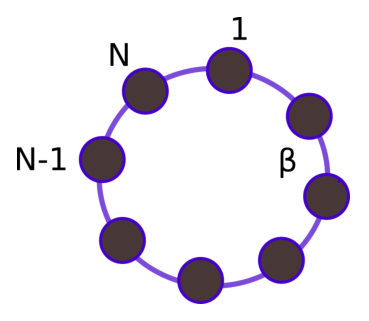
\includegraphics[height=4cm]{cap3/figs/ring_nodist_solo.eps}
\caption{Anillo de N átomos de H.} 
\label{anillo_equi}
\end{figure}

\newpage

Utilizando $c_j= e^{ij\theta}$ e incluyendo la constante de normalización $\frac{1}{N^{1/2}}$ obtenemos:

\begin{equation}
\ket \Psi = \frac{1}{N^{1/2}} \sum_{j=1}^N e^{ij\theta} \ket j
\label{eq:molecular}
\end{equation}

donde el estado s sobre el átomo j se representa con el ket $\ket j$ y el número cuántico $\displaystyle \theta = \frac{2m\pi}{N}$ donde m = 0,1,2,...,(N-1). La ecuación \ref{eq:molecular} es una función de Bloch y se deriva de la simetría traslacional del anillo, en otras palabras, todos los átomos en el anillo son equivalentes por una simple traslación alrededor del anillo. Los valores permitidos de $\theta$ derivan de la periodicidad del estado molecular, es decir, c$_N$ = c$_0$ y c$_{N+1}$ = c$_1$. 

Insertando la ecuación \ref{eq:molecular} en la ecuación de Schr\"odinger $H \ket \Psi = E \ket \Psi $, obtenemos:

\begin{equation}
\sum_{j=1}^N e^{ij\theta} H \ket j = E \sum_{j=1}^N e^{ij\theta} \ket j
\end{equation}

y multiplicando por la izquierda el bra $\bra p$ obtenemos:

\begin{equation}
\sum_{j=1}^N e^{ij\theta}  \bra p H \ket j = E \sum_{j=1}^N e^{ij\theta} \langle p \ket j
\end{equation}

Donde $\langle p \ket j = 0$ excepto cuando $j=p$ asumiendo que la base es ortonormal, entonces:


\begin{equation}
\sum_{j=1}^N e^{ij\theta}  \bra p H \ket j = E e^{ip\theta}
\end{equation}

o, tomando el factor $e^{ip\theta}$ en el lado izquierdo de la igualdad:

\begin{equation}
\sum_{j=1}^N e^{i(j-p)\theta}  \bra p H \ket j = E({\theta})
\end{equation}

Los elementos de matriz $\bra p H \ket j$ son nulos excepto cuando $j=p$ o $j = p+1$ o $j = p-1$. Cuando $j=p$ obtenemos los elementos de matriz \emph{on site} $\bra p H \ket j = \alpha$ y cuando $j = p+1$ o $j = p-1$ obtenemos los elementos de matriz entre átomos vecinos (integrales de \emph{hopping} o simplemente \emph{hopping}) $\bra p H \ket j = \beta$. Entonces hay solo 3 términos en la suma de la izquierda que no son nulos:

\begin{equation}
\alpha + \beta e^{i\theta} + \beta e^{-i\theta} = \alpha + 2\beta \cos{\theta} = E
\end{equation}

En cristales de una dimensión (1D) el GAP es introducido por distorciones periódicas llamadas distorciones de Peierls. Considerando un anillo de átomos equiespaciados (distancia = a) y \emph{hopping} $\beta$ generamos la banda prohibida al mover los átomos del anillo con el objetivo de generar 2 distancias interatómicas alternadas (a y b) y por ende 2 \emph{hopping} $\beta_1$ y $\beta_2$ como se muestra en la figura \ref{anillo_dist}. Las distorciones de Peierls se asemejan a una molécula de poliacetileno donde se intercalan enlaces simples y dobles. 

\begin{figure}[!htb]
\centering
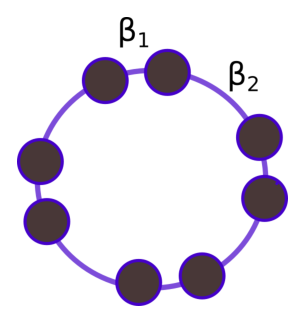
\includegraphics[height=4cm]{cap3/figs/ring_dist_solo.eps}
\caption{Anillo distorcionado con hopping electrónicos $\beta_1$ y $\beta_2$.} 
\label{anillo_dist}
\end{figure}

El complejo en cuestión simulado con un modelo TB es el que se muestra en la figura \ref{anillo_dist_mol}. El anillo puede acoplarse en distintos grados a una molécula diatómica, lo cual está regulado por el parámetro $\gamma$. La interacción entre los ́atomos de la molécula se representa con el parámetro $\delta$, por lo que la transición electrónica tiene una energía de 2 $\delta$. El centro de energía de la diatómica respecto al centro del GAP del semiconductor está representado por el parámetro $\epsilon$. Los \emph{hopping} electrónicos $\beta_1$ y $\beta_2$ son una medida de las interacciones entre los átomos del anillo y por esta razón regulan el GAP. Por último, otro de los parámetros que se tiene en cuenta a la hora de la simulación, es $\mu$, el cual define el potencial electroquímico de los electrones en todo el sistema con una temperatura tal que $kT = 0.001$ Ha.

\begin{figure}[!htb]
\centering
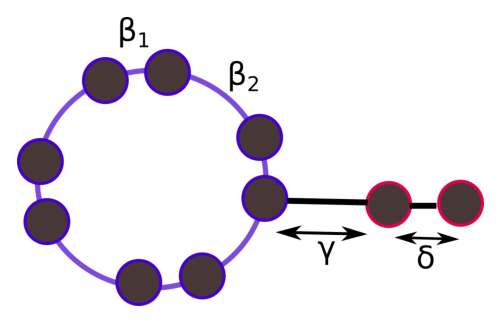
\includegraphics[height=4cm]{cap3/figs/ring_dist.eps}
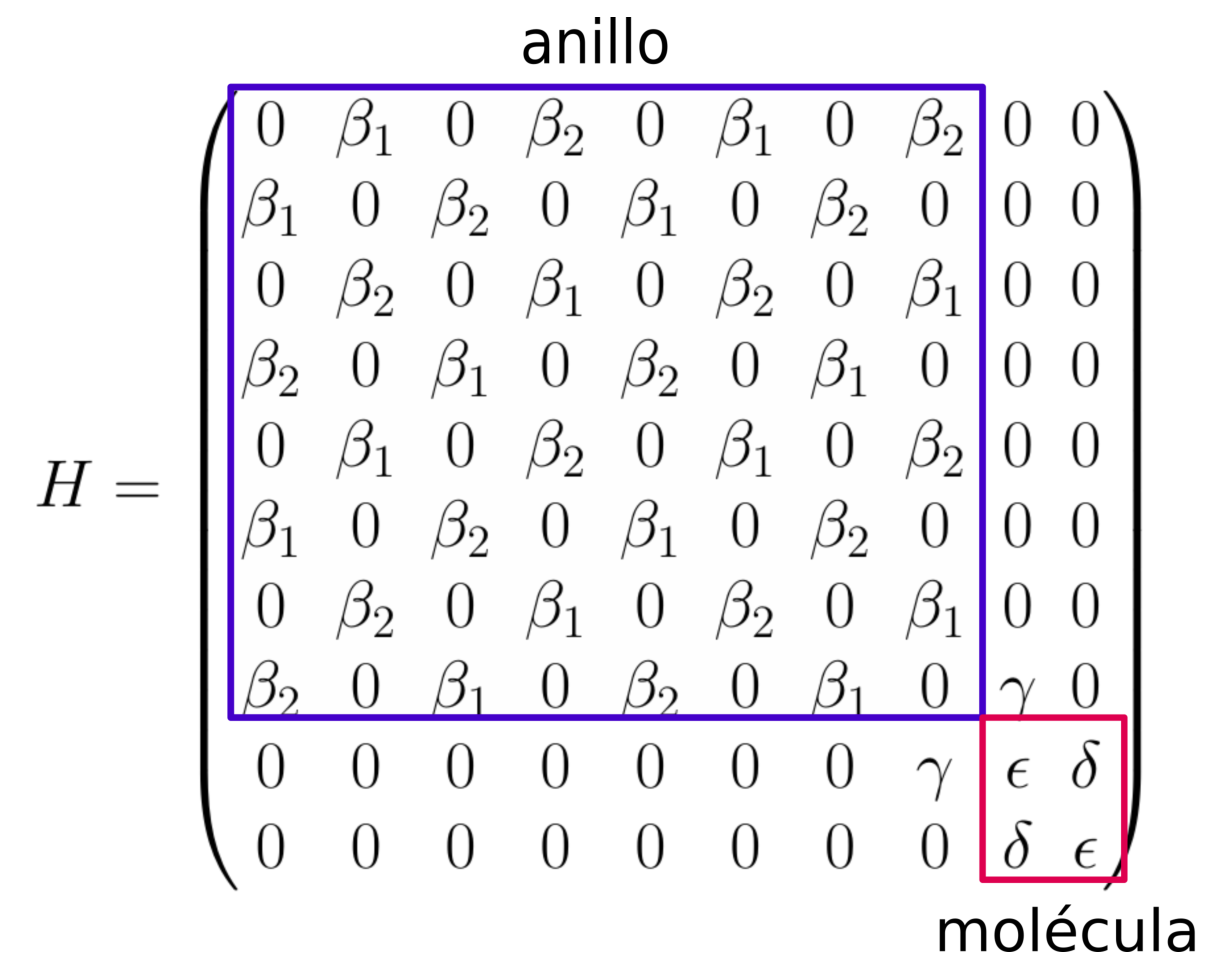
\includegraphics[height=4.5cm]{cap3/figs/h_1.eps}
\caption{\textbf{Izquierda} Esquema del anillo semiconductor acoplado a una diatómica. \textbf{Derecha} hamiltoniano para un sistema N=10.} 
\label{anillo_dist_mol}
\end{figure}

El hamiltoniano modelo es de electrones independientes y por tanto desprecia completamente los efectos de las interacciones inter-electrónicas, tanto de intercambio como coulómbicas. La inclusión de interacción electrón-electrón a campo medio (en un modelo autoconsistente) será objeto de un trabajo posterior. El efecto fundamental de la interacción electrón-electrón en estos sistemas, en base a la experiencia adquirida en el grupo en los últimos años, se reduce a una renormalización de las energías de excitación y velocidades de transferencia electrónica. Dado que el objetivo del modelo es lograr una descripción cualitativa del fenómeno se priorizó la simplicidad del hamiltoniano para facilitar la comprensión de los resultados y posibilitar una exploración extensiva del espacio de parámetros. Es importante aclarar que no se tiene en cuenta la disipación térmica de los núcleos, en este modelo sólo se considera el movimiento electrónico.

El hamiltoniano fue calculado a través de una matriz NxN (N = número de atomos del sistema) con dos bloques principales, uno que representa al SC y otro a la molécula. En la figura \ref{anillo_dist_molohenberg1964} a la derecha se muestra el hamiltoniano cuando N = 10. El bloque del hamiltoniano correspondiente al SC tiene dimensiones N-2 x N-2 con elementos de matriz nulos cuando i = j $\pm$ 2n mientras que para i= j+(2n $\pm$ 1) se muestran los \emph{hopping} de forma alternada.

El bloque de la diatómica tiene dimensiones 2x2 debido a los orbitales H-L. El parámetro $\epsilon$ conforma la diagonal y en el resto del bloque se encuentra $\delta$. El acoplamiento, $\gamma$, se encuentra en H$_{N−2,N−3}$ y H$_{N−3,N−2}$, entre los dos bloques.

\subsection{Cálculo de la densidad de estados}

Suponiendo que tenemos todos los autoestados $\ket n$ y las energías E$_n$ de un hamiltoniano electrónico simple, se define a la densidad total de estados para un sistema finito DOS(E) por la relación: 

\begin{equation}
\label{dos_finito}
\displaystyle DOS (E) = \sum_n \frac{1}{\sqrt{2}}  e^{\frac{(E-E_n)^ 2}{\sigma^2}}
\end{equation}

donde $\sigma$ es el ancho de una función gaussiana.

Esto debe entenderse en el sentido operacional, que si integramos la DOS(E) sobre un rango de energía, obtenemos el número total de estados dentro del mismo \cite{finnis}. Para sistemas infinitos la densidad de estados se calcula mediante funciones delta de Dirac pero cuando se trata de sistemas finitos, como el planteado en el presente capítulo, se ensanchan las deltas de Dirac utilizando funciones gaussianas para cada una de las energías.


\subsection{Cálculo del espectro de absorción}

La expresión general de la función respuesta lineal para un gas de electrones no interactuantes \cite{giuliani}: 

\begin{equation}
\label{espectro_general}
\chi_{AB}^{(0)} = \sum_{\alpha\beta} \frac{n_\alpha- n_\beta}{\hbar+ \epsilon_\alpha- \epsilon_\beta + i\hbar\eta} A_{\alpha \beta} B_{\beta \alpha}
\end{equation}

donde $n_\alpha$ y $n_\beta$ es la ocupación promedio Fermi-Dirac del estado $\alpha$ y el estado $\beta$, respectivamente a temperatura T y potencial electroquímico $\mu$ de los electrones, $\epsilon$$_\alpha$– $\epsilon$$_\beta$ es la diferencia de energía entre los estados $\alpha$ y $\beta$ y A$_{\alpha \beta}$, B$_{\beta \alpha}$  son los elementos de matriz de los operadores A y B. 

A los fines de describir el espectro de absorción, se calculó la función de respuesta lineal, donde los operadores A y B son en este caso, los operadores momento dipolar de transición $\mu$$_{\alpha\beta}$ y $\mu$$_{\beta\alpha}$ (ver ecuación \ref{espectro}) los cuales otorgan el peso a la transición.

Los términos $n$$_\alpha$ y $n$$_\beta$ indican que cuando los estados $\alpha$ y $\beta$ están ambos ocupados o desocupados, el numerador de la ecuación es cero y por ende también el término de la sumatoria. De esta forma, las únicas transiciones que se toman en cuenta a la hora del cálculo del espectro, son las de estado ocupado a desocupado.

\begin{equation}
\label{espectro}
\chi_{\mu_{\alpha\beta} \mu_{\beta \alpha}}^{(0)} = \sum_{\alpha\beta} \frac{n_\alpha- n_\beta}{\hbar+ \epsilon_\alpha- \epsilon_\beta + i\hbar\eta} {\mid{{\mu _{\alpha\beta}}}\mid} ^{2}
\end{equation}
 
\subsection{Cálculo de transferencia de carga}

Para estudiar la transferencia de carga fue necesario calcular la dinámica electrónica del sistema bajo la acción de un láser.  Se procedió, en primera instancia, a diagonalizar el hamiltoniano para calcular la matriz de autovectores y de esa forma calcular el operador matriz densidad monoelectrónica $\hat{\rho}$. Para realizar el cálculo de la transferencia de carga se aplica una perturbación con forma de función sinusoidal $E(t) = E_0 \sen{(\omega t)}u$, donde $E_0$ es la intensidad del campo y $\omega$ la frecuencia de excitación de interés. 

Cuando se perturba a partir de t = 0 el operador $\hat{\rho}$, se inicializa la dinámica. La integración numérica para obtener la propagación electrónica se realiza a partir del algoritmo:

\begin{equation}
 \label{leapfrog}
  \hat{\rho}(t+\delta t) = \hat{\rho}(t-\delta t) + 2 \delta t \frac{\partial \hat{\rho}(t)}{\partial t}  
\end{equation}

donde $\hat{\rho}(t + \delta t)$ es el operador matriz densidad propagado en el tiempo, $\hat{\rho}(t - \delta t)$ es el operador matriz densidad en el paso anterior y $\frac{\partial \hat{\rho}(t)}{\partial t}$ es la derivada parcial del operador matriz densidad con respecto al tiempo, este último se obtiene a partir de la ecuación de Liouville-von Newmann:

\begin{equation}
 \label{newman}
  \frac{\delta \hat{\rho}}{\delta t}= \frac{1}{i\hbar} (\hat{H}\hat{\rho} - \hat{\rho}\hat{H})
\end{equation}


donde $\hat{\rho}$ es el operador matriz densidad y $\hat{H}$ es el operador Hamiltoniano.

En este caso la intensidad del campo llevó al sistema fuera del régimen de respuesta lineal, ya que se buscó sacar al sistema del equilibrio y ver el posible movimiento de los electrones en el tiempo. Luego del cálculo de la dinámica se procede a analizar/graficar la variación de las poblaciones electrónicas con respecto al tiempo ya que de esta forma podemos observar indirectamente la transferencia de carga.

\section{Simulación de complejos colorante-SC utilizando el modelo propuesto.}

Utilizando el modelo propuesto se calcularon y estudiaron: densidad de estados o DOS, espectros de absorción y transferencia de carga en complejos diatómica-anillo. Para llevar a cabo dichas tareas fue necesario variar uno o varios de los parámetros del modelo mientras los restantes se mantuvieron constantes y luego se analizó el comportamiento del sistema en respuesta a los cambios que se generaron. De esta forma, se realizó el procedimiento con cada uno de los parámetros de interés para obtener una mirada general del modelo bajo estudio.

A través de investigaciones que se realizaron en el grupo, se conoce que los SC utilizados en las DSSC tienen un GAP de aproximadamente 3 eV (zona del ultravioleta) mientras que el colorante, como absorbe en el visible, tiene una diferencia energética H-L promedio de 2 eV. Con el fin de que el modelo represente situaciones lo más reales posibles, se tomaron ciertos valores para los parámetros que respeten la relación $\frac{3}{2}$ de energía de absorción entre el SC y la molécula diatómica. Por ello, a lo largo de todo del capítulo, se utilizaron los valores de \emph{hopping} electrónicos $\beta_1= -0.5$ y $\beta_2= -1.0$ para el SC que definen un GAP de 1 u.a. de acuerdo a la relación $ GAP = 2\mid{\alpha-\beta}\mid$ y $ 2\delta = -0.6$ como valor de energía necesaria para la transición de la diatómica.

Los parámetros que se fueron modificando para realizar el análisis fueron: $\epsilon$ ya que posiciona energéticamente los orbitales HOMO-LUMO de la diatómica con respecto al centro del GAP del SC, $\mu$ que determina el potencial electroquímico de los electrones en el sistema y $\gamma$ que establece el acoplamiento entre la molécula y el SC.


\subsection{Sistema sin acoplamiento}

Una molécula pueda considerarse un buen sensibilizador en una DSSC si cumple con diversos requisitos, entre otros, que absorba en la región visible del espectro e incluso en el infrarrojo cercano. En las DSSC más comunes (por ejemplo las celdas de Gr\"atzel \cite{ORegan1991}) el LUMO o nivel de energía del estado excitado del fotosensibilizador debe ser mayor en energía que la energía del borde de la banda de conducción (BC) del semiconductor (SC). También se ha demostrado la existencia de DSSC en las que el HOMO del colorante se encuentra ubicado energéticamente en la BV del SC \cite{Negre2014,Borgstrom2005}.
 
Como punto de partida, se consideró el sistema colorante - SC sin acoplamiento, dicho de otro modo, {\bf $\gamma=0$}, para corroborar la eficacia del modelo en un amplio espectro de situaciones. Tomando $\gamma$ como parámetro fijo, se utilizaron valores de $\epsilon$ y $\mu$ tal que garanticen 2 situaciones particulares: \textbf{(1-e)} el LUMO de la molécula se encuentre energéticamente dentro de la BC del SC y \textbf{(1-h)} el HOMO de la molécula se encuentre energéticamente dentro de la banda de valencia (BV) del SC. Para evaluar el sistema \textbf{(1-e)} se utilizaron los parámetros $\epsilon=0.45$ y $\mu=0.3$ y para el sistema \textbf{(1-h)} se utilizaron los parámetros $\epsilon=-0.45$ y $\mu=-0.3$

\begin{figure}[!htb]
 \centering
 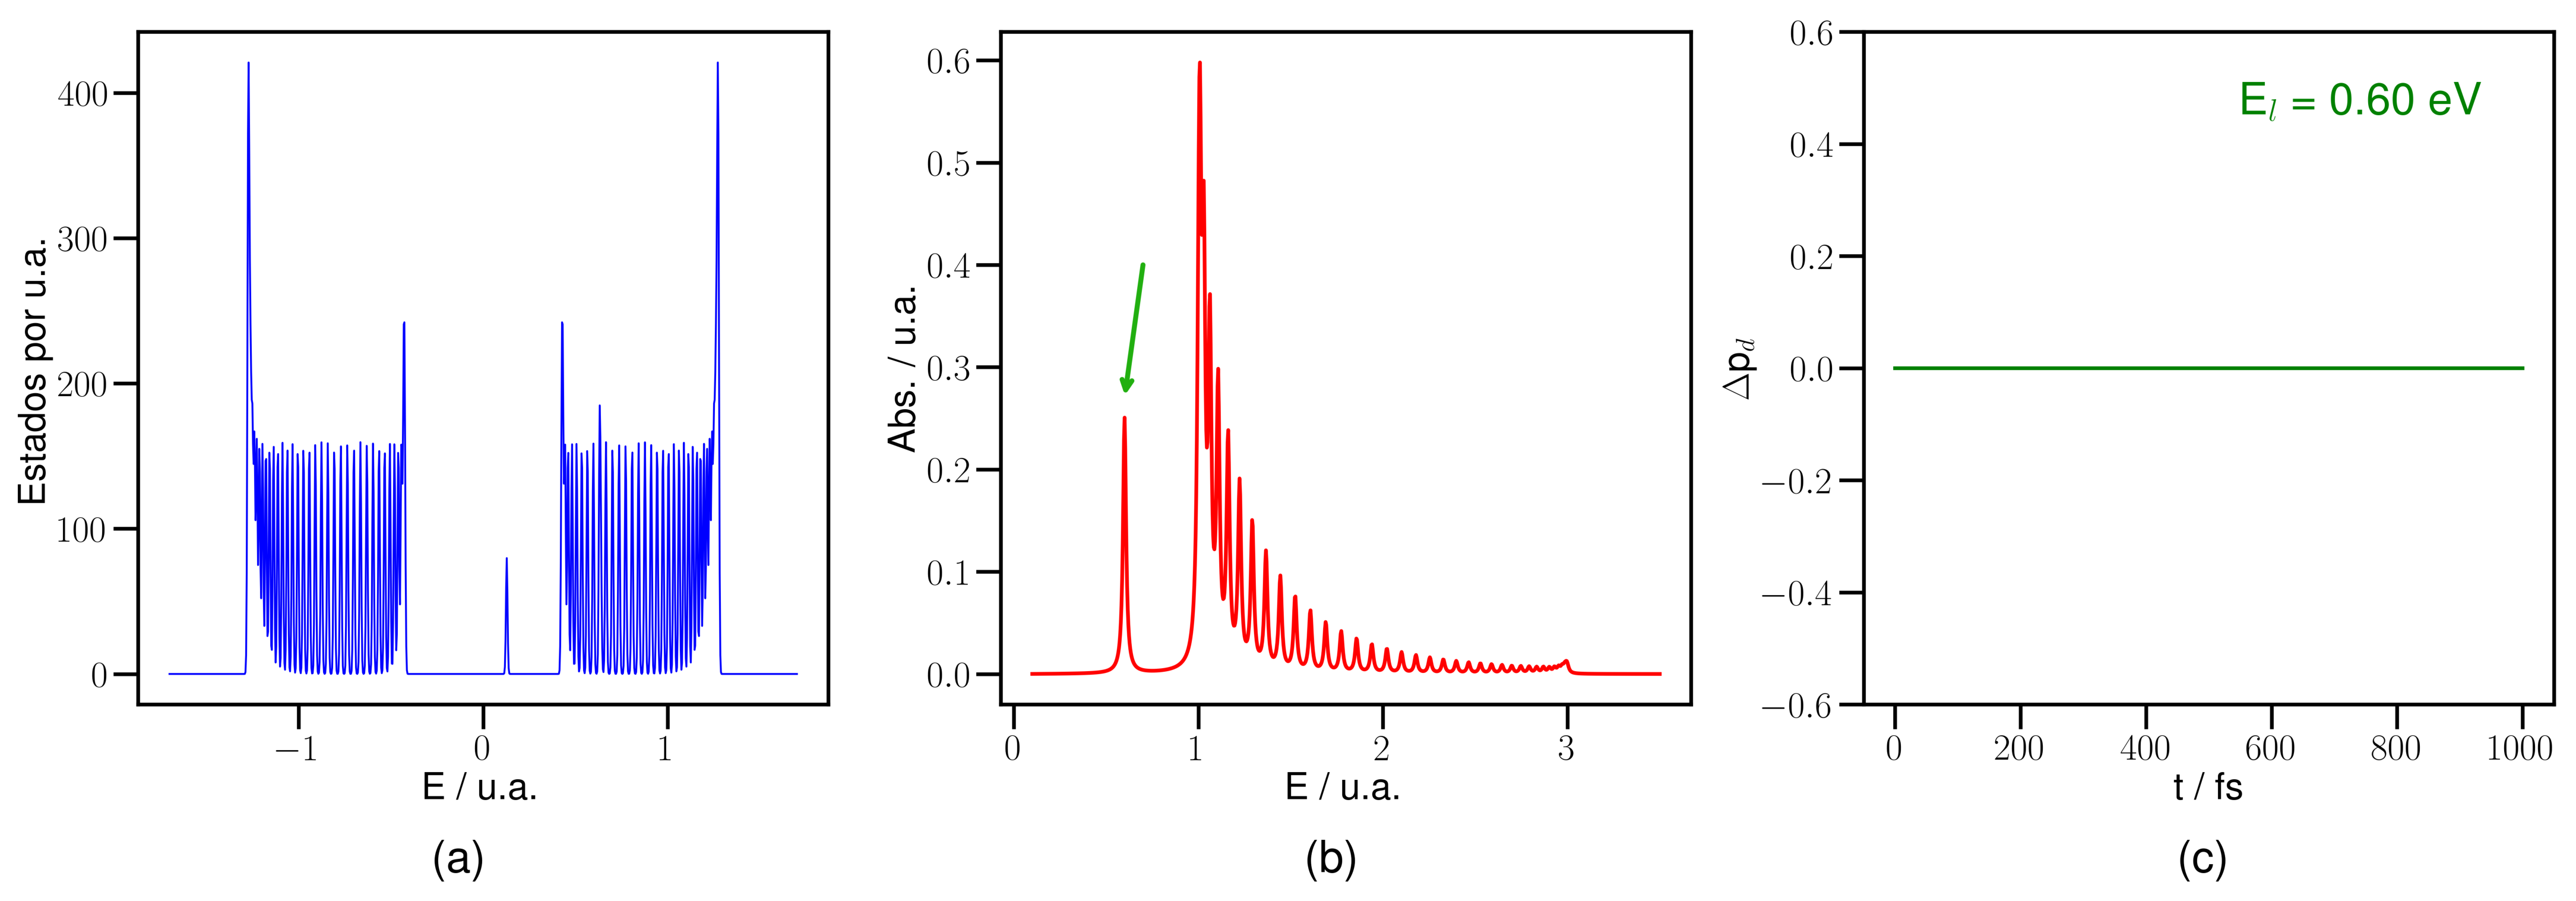
\includegraphics[height=5cm]{cap3/figs/fig_s_acople_diat.eps}
 \caption{Sistema \textbf{(1-e)}. \textbf{(a)} DOS, \textbf{(b)} espectro de absorción y \textbf{(c)} diferencia de población en la diatómica respecto a la población inicial ($\Delta p_d$) en función del tiempo aplicando un campo electromagnético con energı́a $0.6$ u.a.}
 \label{1-e}
\end{figure}


Los gráficos de la figura \ref{1-e} corresponden a los resultados para los cálculos del sistema \textbf{(1-e)}. En el gráfico de la DOS {\textbf{(a)} se observa por un lado el HOMO de la diatómica a $0.15$ u.a. de acuerdo al parámetro $\delta = 0.3$ elegido. El LUMO no se observa a simple vista debido a que se encuentra energéticamente dentro de la BC. Por otro lado, las 2 bandas del SC, a menor energía la BV y a mayor energía la BC separadas por un GAP de 1 u.a. Se puede observar también el nivel de Fermi en cero, entre la BV y BC, que junto con el GAP representan los parámetros típicos de un SC. Como el mismo posee bandas (a diferencia de la molécula), tiene una gran cantidad de estados disponibles para las transiciones.

El espectro de absorción del sistema con acoplamiento nulo \textbf{(b)} muestra un pico a aproximadamente $0.6$ u.a. de intensidad moderada y una banda a mayor energía en el rango $1-1.5$ u.a. con una intensidad mayor. Como ya se mencionó anteriormente, la diatómica puede solamente sufrir transiciones entre los orbitales H-L mientras que en el SC cualquier electrón que cuente con la energía necesaria puede excitarse desde la BV a la BC, por ello el pico del espectro corresponde a la absorción de la molécula y la banda al SC. La energía necesaria para que ocurra la transición H-L de la diatómica es mucho menor que la requerida para que ocurra la transición BV-BC del SC. Este comportamiento se debe a que la relación $\frac{3}{2}$ entre las energías de absorción de la diatómica y el SC se corresponde con DSSC reales en las que el colorante aislado absorbe en el visible y el SC aislado en el ultravioleta (por ejemplo complejos colorante-TiO$_2$). La energía necesaria para que ocurra una transición en el visible es menor que la necesaria para que ocurra en el ultravioleta, lo cual se encuentra plasmado en el espectro. Tambien se observa en la banda del SC, picos con distintas intensidades. La transición que genera la máxima intensidad en el espectro es la que ocurre desde el último nivel de energía de la BV al primer nivel de energía de la BC porque es el proceso menos energético mientras que los picos menos intensos son producto de transiciones que requieren más energía. Contribuye también a la intensidad de los picos el hecho de que las densidades de estado al borde de banda son máximas.

Para estudiar la transferencia de carga del sistema \textbf{(1-e)} sin acoplamiento fue necesario aplicar una perturbación continua de tipo láser con la energı́a de la transición de interés. Los parámetros utilizados para la dinámica electrónica fueron: paso de tiempo $0.01$ fs, número de pasos 100000 e intensidad del campo aplicado $0.01$ V /$\AA$. Como se mencionó anteriormente, la transferencia de carga se deduce indirectamente a través del gráfico de la evolución temporal de la población electrónica en la molécula diatómica ($\Delta p_d$) a medida que se perturba con el láser. 

En la figura \ref{1-e} {\textbf{(c)} se muestra $\Delta p_d$ en función del tiempo al iluminar el complejo molécula-SC con un láser sintonizado con la energía H-L de la diatómica ($0.6$ u.a.). En este caso los electrones de la molécula no se transfieren al SC, en otras palabras, no se observa transferencia de carga neta debido al acoplamiento nulo entre los mismos. En su lugar hay movimiento de electrones al perturbar con las distintas frecuencias de absorción.

\begin{figure}[!htb]
 \centering
 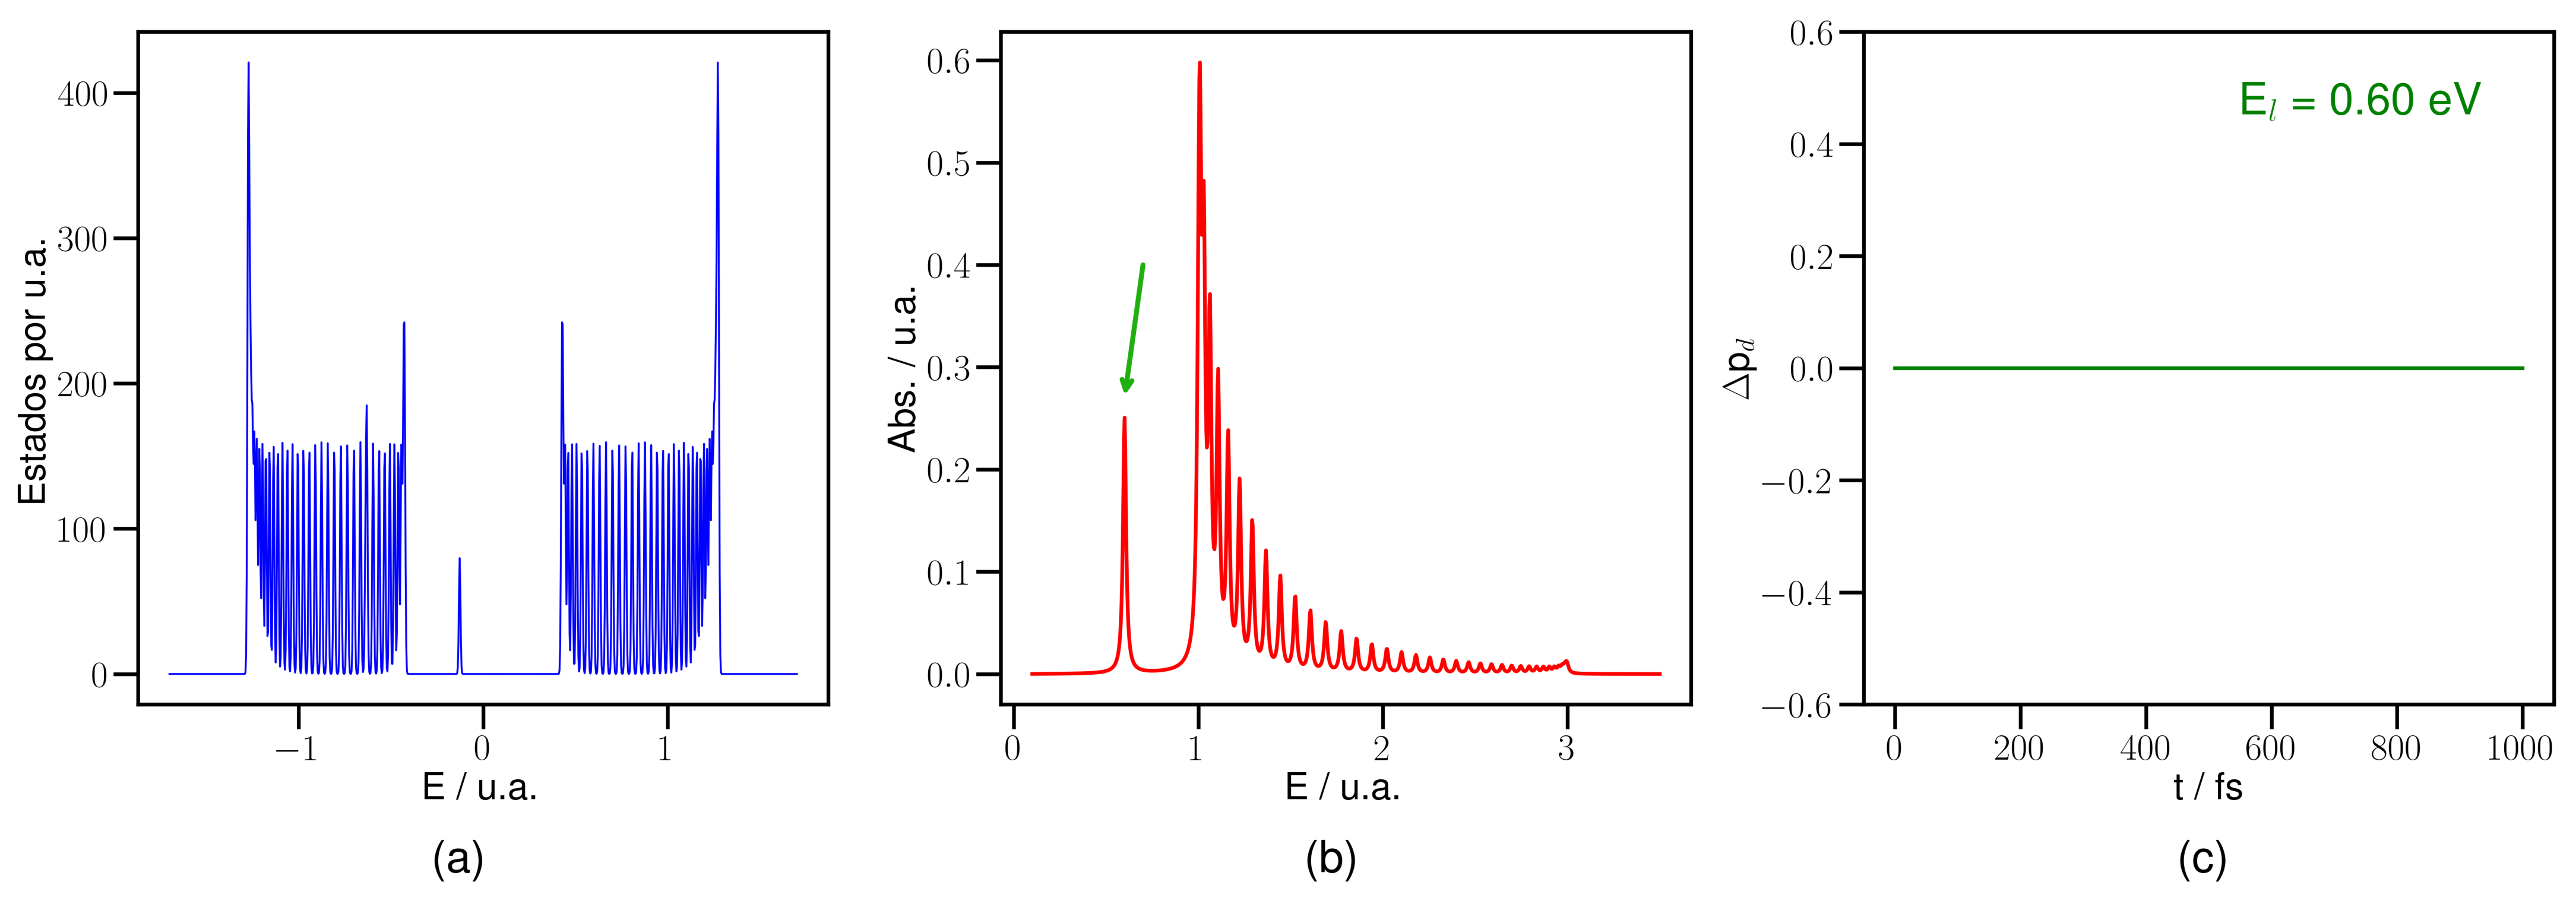
\includegraphics[height=5cm]{cap3/figs/fig_s_acople_diat_hueco.eps}
 \caption{Sistema \textbf{(1-h)}. \textbf{(a)} DOS, \textbf{(b)} espectro de absorción y \textbf{(c)} diferencia de población en la diatómica respecto a la población inicial ($\Delta p_d$) en función del tiempo aplicando un campo electromagnético con energı́a $0.6$ u.a.}
 \label{1-h}
\end{figure}

Los gráficos de la figura \ref{1-h} corresponden a los resultados para los cálculos del sistema \textbf{(1-h)}. En este caso los gráficos de \textbf{(b)} y \textbf{(c)} permanecen iguales al sistema \textbf{1-e}. El cambio en los parámetros $\epsilon$ y $\mu$ afecta a la molécula diatómica y se ve reflejado en el gráfico de la DOS \textbf{(a)}. A diferencia del sistema \textbf{(1-e)} se observa el LUMO de la molécula a $-0.15$ u.a. debido a que el HOMO se encuentra energéticamente dentro de la BC. El pico de la diatómica en el espectro de absorción \textbf{(b)} se encuentra también a $0.6$ u.a. ya que el parámetro $\delta$ que determina la energía de excitación H-L se conserva y la transferencia de carga sigue siendo cero por el acoplamiento nulo. 

%\newpage

\subsection{Sistema con acoplamiento}

El impacto del acoplamiento se evaluó considerando los mismos parámetros que se utilizaron en los sistemas \textbf{1-e} y \textbf{1-h} pero cambiando $\gamma=0$ por $\gamma=0.1$. Los complejos acoplados serán llamados \textbf{2-e} ($\epsilon=0.45$ y $\mu=0.3$) y \textbf{2-h} ($\epsilon=-0.45$ y $\mu=-0.3$). 

\begin{figure}[!htb]
 \centering
 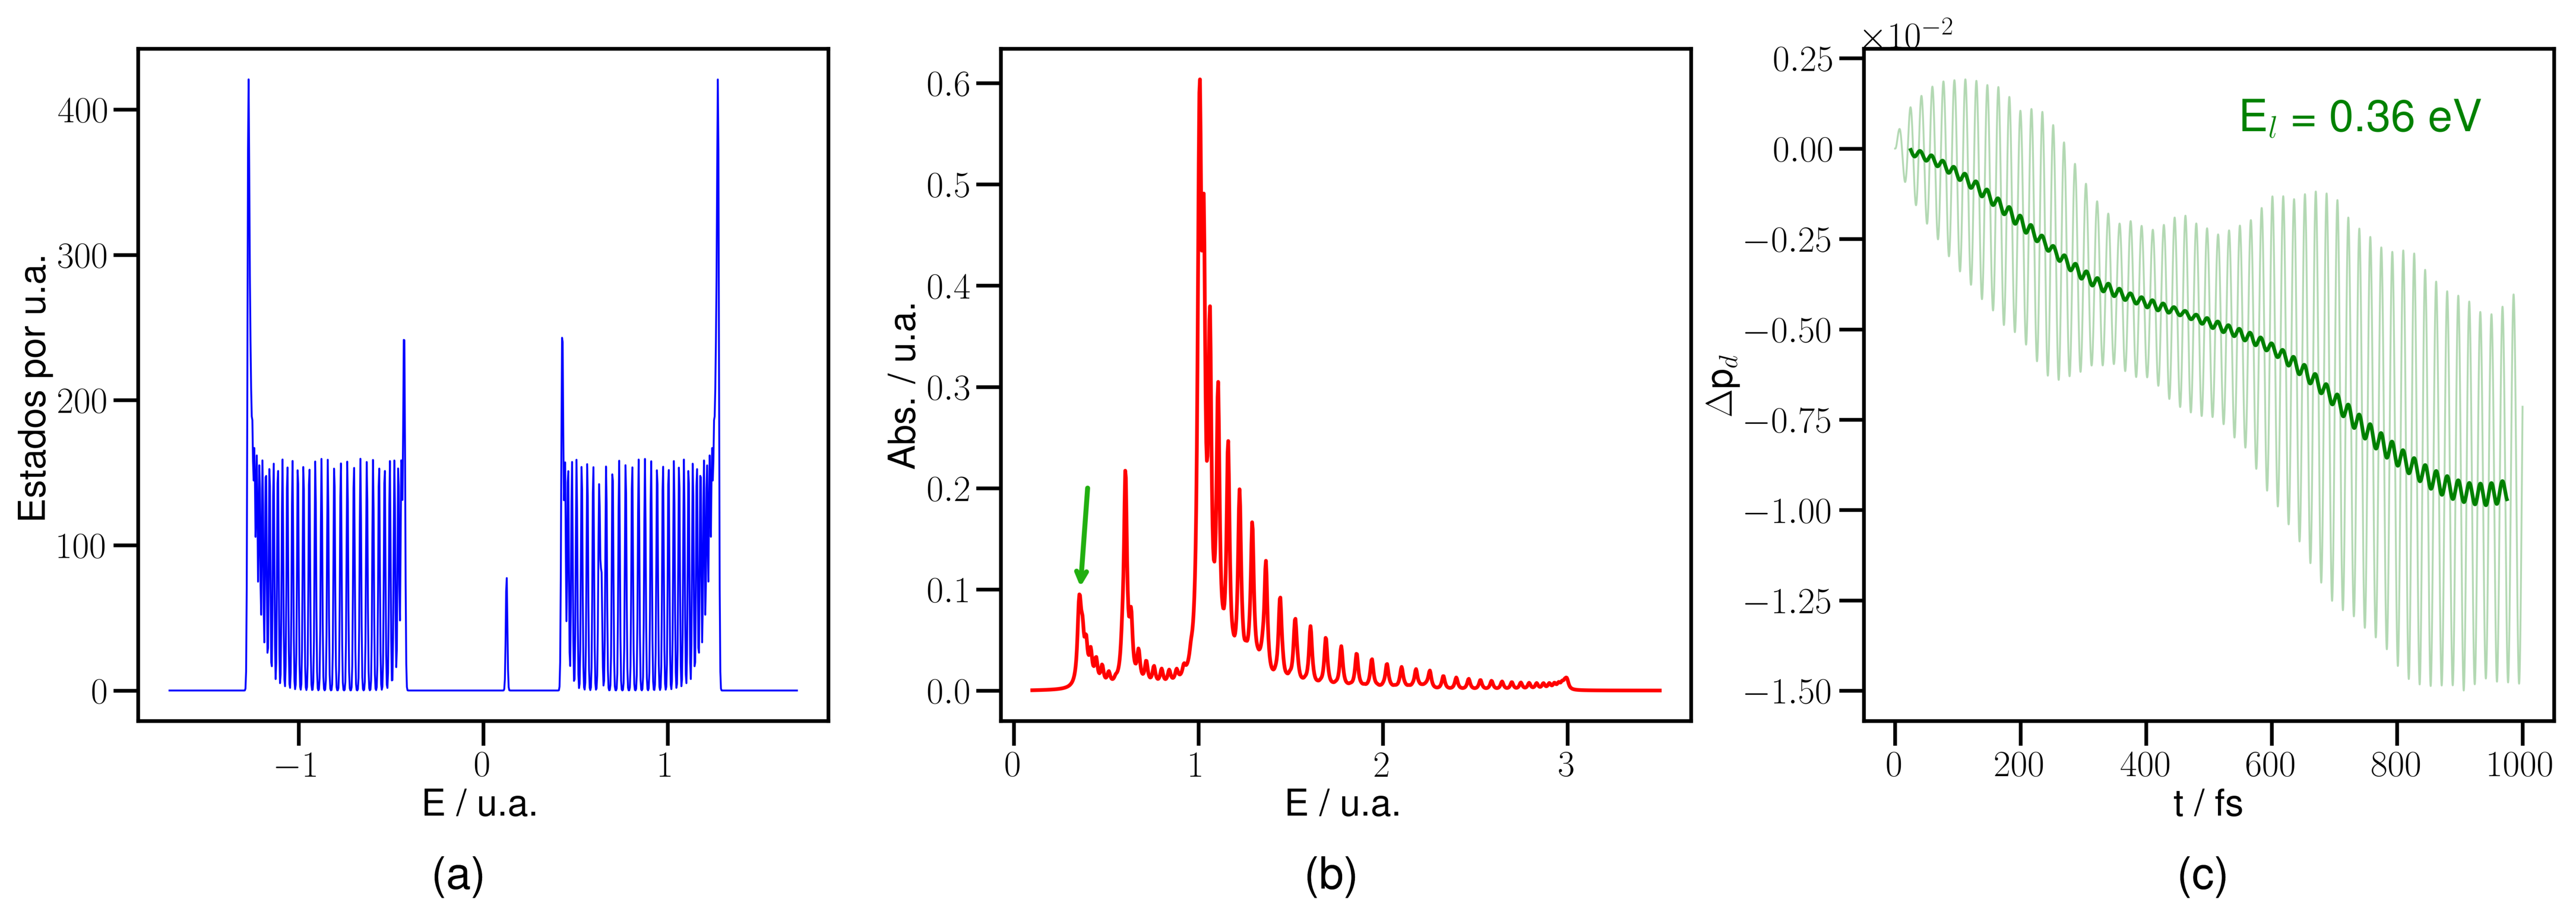
\includegraphics[height=4.8cm]{cap3/figs/fig_c_acople_ghost.eps}
 \caption{Sistema \textbf{(2-e)}. \textbf{(a)} DOS, \textbf{(b)} espectro de absorción y \textbf{(c)} diferencia de población en la diatómica respecto a la población inicial ($\Delta p_d$) en función del tiempo aplicando un campo electromagnético con energı́a $0.36$ u.a.}
 \label{2-e}
\end{figure}


La figura \ref{2-e} presenta los gráficos que se obtuvieron de las simulaciones del sistema \textbf{2-e}. La DOS \textbf{(a)} de este complejo no muestra cambios con respecto a la DOS del sistema sin interacción \textbf{1-e} porque los estados de la molécula y del SC son los mismos a pesar del acoplamiento.


En el espectro del sistema acoplado \textbf{(b)} se observan, nuevamente, el pico y la banda que corresponden a la absorción de la diatómica y el SC respectivamente. No obstante, aparece una nueva banda de menor intensidad y de menor energía en relación a las otras bandas presentes, que indica la aparición de nuevas transiciones en el sistema debidas al acoplamiento. De acuerdo con el potencial electroquímico de los electrones en el sistema ($\mu=0.3$) y con la ubicación energética de la diatómica ($\epsilon= 0.45$), el HOMO cuenta con electrones disponibles para las transiciones. Los mismos pueden excitarse hacia el LUMO o hacia la BC, lo cual está permitido por el acoplamiento incorporado. La nueva transición posible que surge de acoplar la diatómica con el SC ocurre desde el HOMO a la BC del SC (H-C) y se observa en el espectro como una banda a $0.36$ u.a. 

La evolución temporal de $\Delta p_d$ a medida que se ilumina con un láser con la energía de transición H-C ($0.36$ u.a.) se muestra en \textbf{(c)}. Es importante aclarar que las oscilaciones rápidas que se observan en la carga corresponden al período de oscilación del láser. La población de electrones disminuye con el tiempo debido a la perturbación, indicando la inyección de electrones a través de un proceso directo, desde el HOMO a la BC. La disminución de $\Delta p_d$ indica la transferencia de carga desde la molécula al SC.

Los resultados señalan entonces que se puede observar transferencia de carga al iluminar el complejo acoplado con una energia menor a la excitación H-L y que ocurre en una sola etapa.


\begin{figure}[!htb]
 \centering
 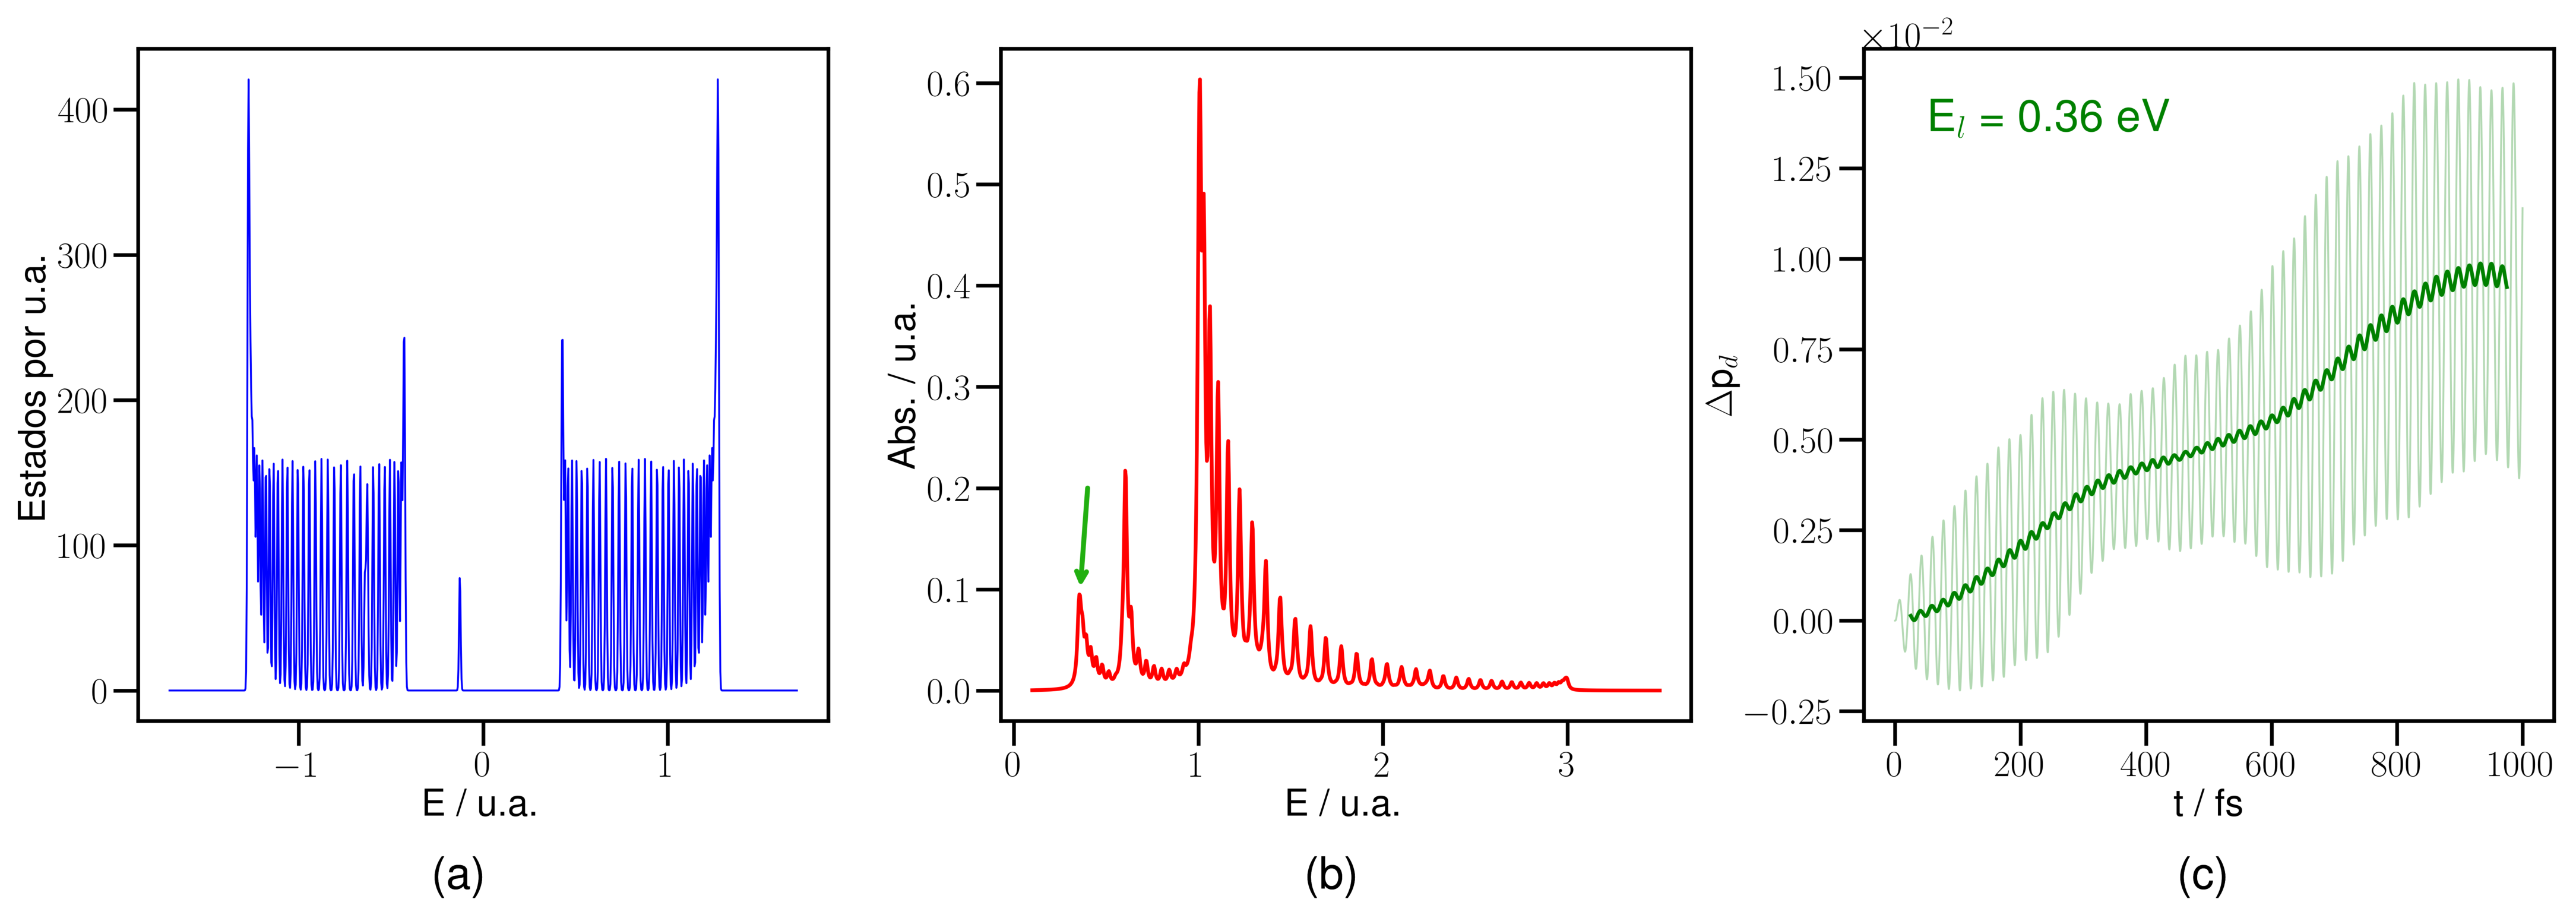
\includegraphics[height=4.8cm]{cap3/figs/fig_c_acople_ghost_hueco.eps}
 \caption{Sistema \textbf{(2-h)}. \textbf{(a)} DOS, \textbf{(b)} espectro de absorción y \textbf{(c)} diferencia de población en la diatómica respecto a la población inicial ($\Delta p_d$) en función del tiempo aplicando un campo electromagnético con energı́a $0.36$ u.a.}
 \label{2-h}
\end{figure}

La figura \ref{2-h} presenta los gráficos que se obtuvieron de las simulaciones del sistema \textbf{2-h}. La DOS \textbf{(a)} tampoco presenta cambios con respecto a la DOS del sistema no acoplado \textbf{1-h}. El espectro de absorción \textbf{(b)} se muestra idéntico al espectro del complejo \textbf{2-e} (ver figura \ref{2-e} \textbf{(b)}) y se debe a la simetría del modelo. Sin embargo, en este sistema, la banda a $0.36$ u.a. corresponde a transiciones que ocurren desde la BV del SC al HOMO de la molécula (V-H), lo cual se puede ver reflejado en el gráfico de $\Delta p_d$ en función del tiempo (ver figura \ref{2-h}\textbf{(c)}) al iluminar el complejo a $0.36$ u.a. La población de electrones aumenta con el tiempo, indicando la transferencia de carga desde el SC a la molécula, es decir en dirección opuesta al sistema \textbf{2-e}. La inyección de electrones al HOMO genera cargas positivas o huecos en el SC.

\subsubsection{Variación del acoplamiento}

Para que se logre una transferencia electrónica efectiva debe haber un buen acoplamiento electrónico entre los orbitales electrónicos del sensibilizador y la BC o BV del SC. Con la finalidad de explorar los efectos de los distintos grados de acoplamiento entre la molécula y el SC se analizaron complejos con $\gamma = 0$, $\gamma = 0.02$, $\gamma = 0.05$ y $\gamma = 0.1$ manteniendo $\epsilon=0.45$ y $\mu=0.30$ constantes, tal como muestra la figura \ref{2-e-g-t}.

\begin{figure}[!htb]
 \centering
 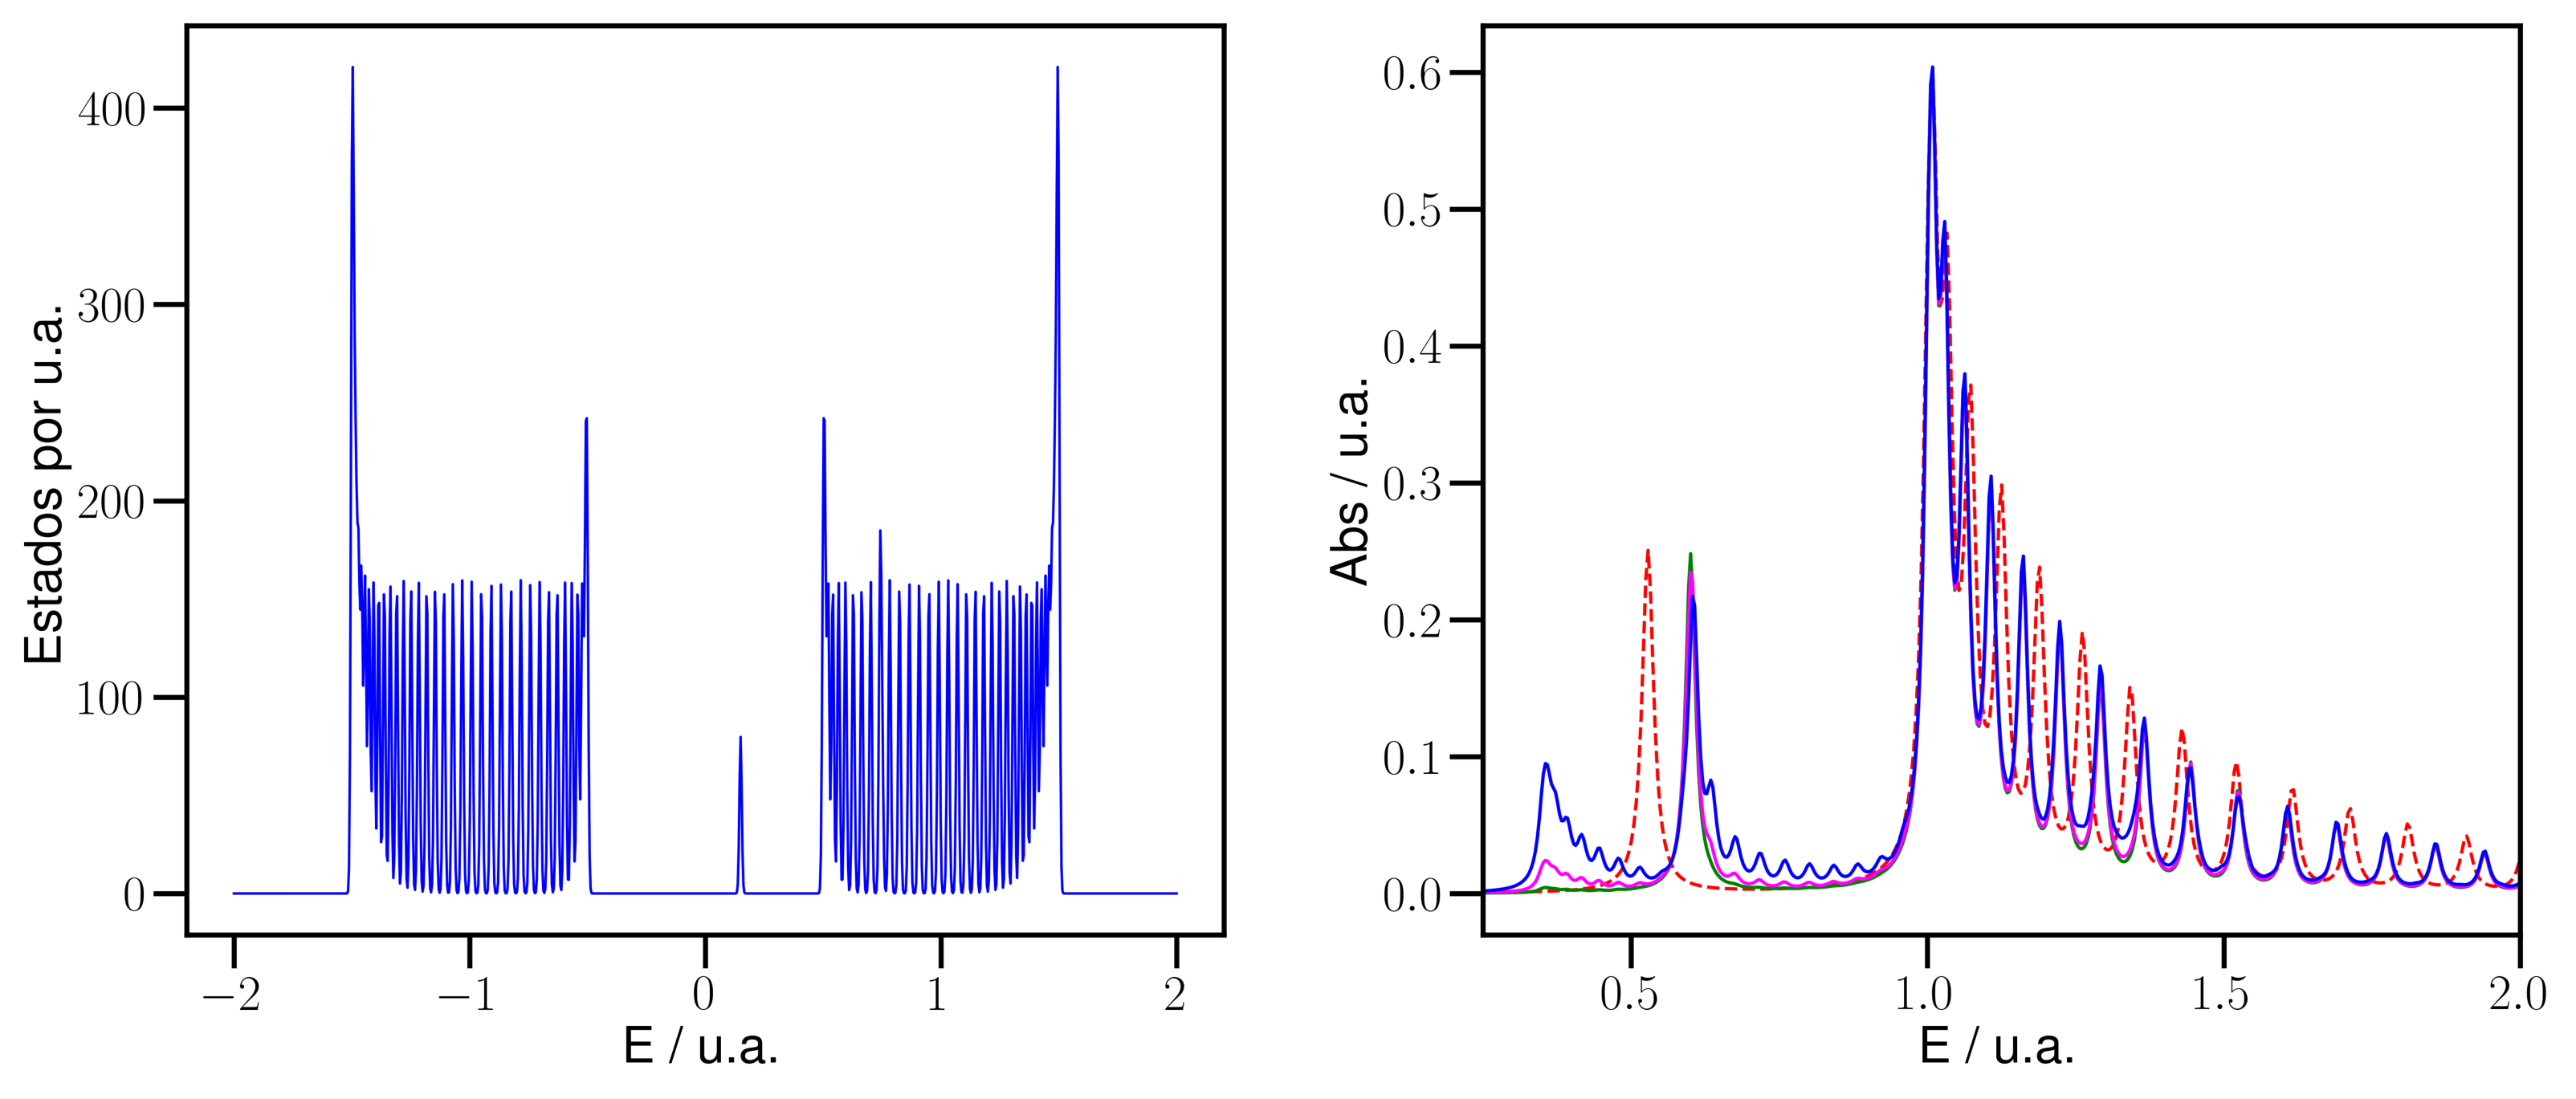
\includegraphics[height=5cm]{cap3/figs/fig_gamas_todo.eps}
 \caption{\textbf{(Izquierda)} DOS y \textbf{(derecha)} espectros de absorción para distintos acoplamientos: $\gamma = 0$, $\gamma = 0.02$, $\gamma = 0.05$ y $\gamma = 0.1$ utilizando $\epsilon=0.45$ y $\mu=0.3$ como parámetros fijos.}
 \label{2-e-g-t}
\end{figure}


\begin{figure}[!htb]
 \centering
 \includegraphics[height=4.3cm]{cap3/figs/fig_gamas_1.eps}
 \caption{Gráficos de \textbf{(a)} Espectro de absorción para distintos $\gamma$ y $\Delta p_d$ en función del tiempo aplicando un campo electromagnético con energı́a $0.36$ u.a. a complejos con distintos acoplamientos: \textbf{(b)} $\gamma = 0.02$, \textbf{(c)} $\gamma = 0.05$ y \textbf{(d)} $\gamma = 0.1$ }
 \label{2-e-g}
\end{figure}

En la figura \ref{2-e-g} \textbf{(a)} se observa el espectro de absorción en el rango ($0.2-0.8$) u.a. para las distintas $\gamma$ seleccionadas. La incorporación del acoplamiento genera por un lado el corrimiento de la banda del colorante a mayores energías, de $0.54$ u.a. a $0.60$ u.a., y por otro la aparición de una nueva banda a $0.36$ u.a. A medida que $\gamma$ crece, la absorción de la molécula disminuye mientras que la absorción de la banda nueva aumenta. Simultáneamente se observa que ambas bandas, la del colorante y la nueva, se parecen cada vez más (en forma) a la banda del SC (ver figura \ref{2-e-g-t}), lo cual deriva del mayor acoplamiento entre los niveles electrónicos. Cuando se utiliza $\gamma = 0.02$ la absorción de la nueva banda es tan pequeña que se considera despreciable.  


En la figura \ref{2-e-g} \textbf{(b)}, \textbf{(c)} y \textbf{(d)} se muestran los gráficos de $\Delta p_d$ en función del tiempo cuando se iluminan los complejos con un láser continuo sintonizado con la energía de la nueva banda ($0.36$ u.a.). En primer lugar se muestra que $\Delta p_d$ aumenta un orden de magnitud a medida que las constantes de acoplamiento crecen. En complejos con acoplamientos menores, como por ejemplo \textbf{(b)}, la transferencia de carga mediante el mecanismo directo es muy pequeña y por ende la contribución a la transferencia de carga total también es pequeña. Sin embargo, la inyección de electrones en la BC también puede ocurrir mediante otro tipo de mecanismo, es decir, la excitación H-L de la molécula y luego la introducción de los electrones en la BC. En la figura \ref{acople_chico} se observa que los valores de $\Delta p_d$ al iluminar con la energía de la molécula o $0.60$ u.a. son mayores con respecto a la iluminación a $0.36$ u.a. Con estos resultados podemos decir que la transferencia ocurre preferentemente mediante un mecanismo indirecto o en 2 etapas. 

\begin{figure}[!htb]
 \centering
 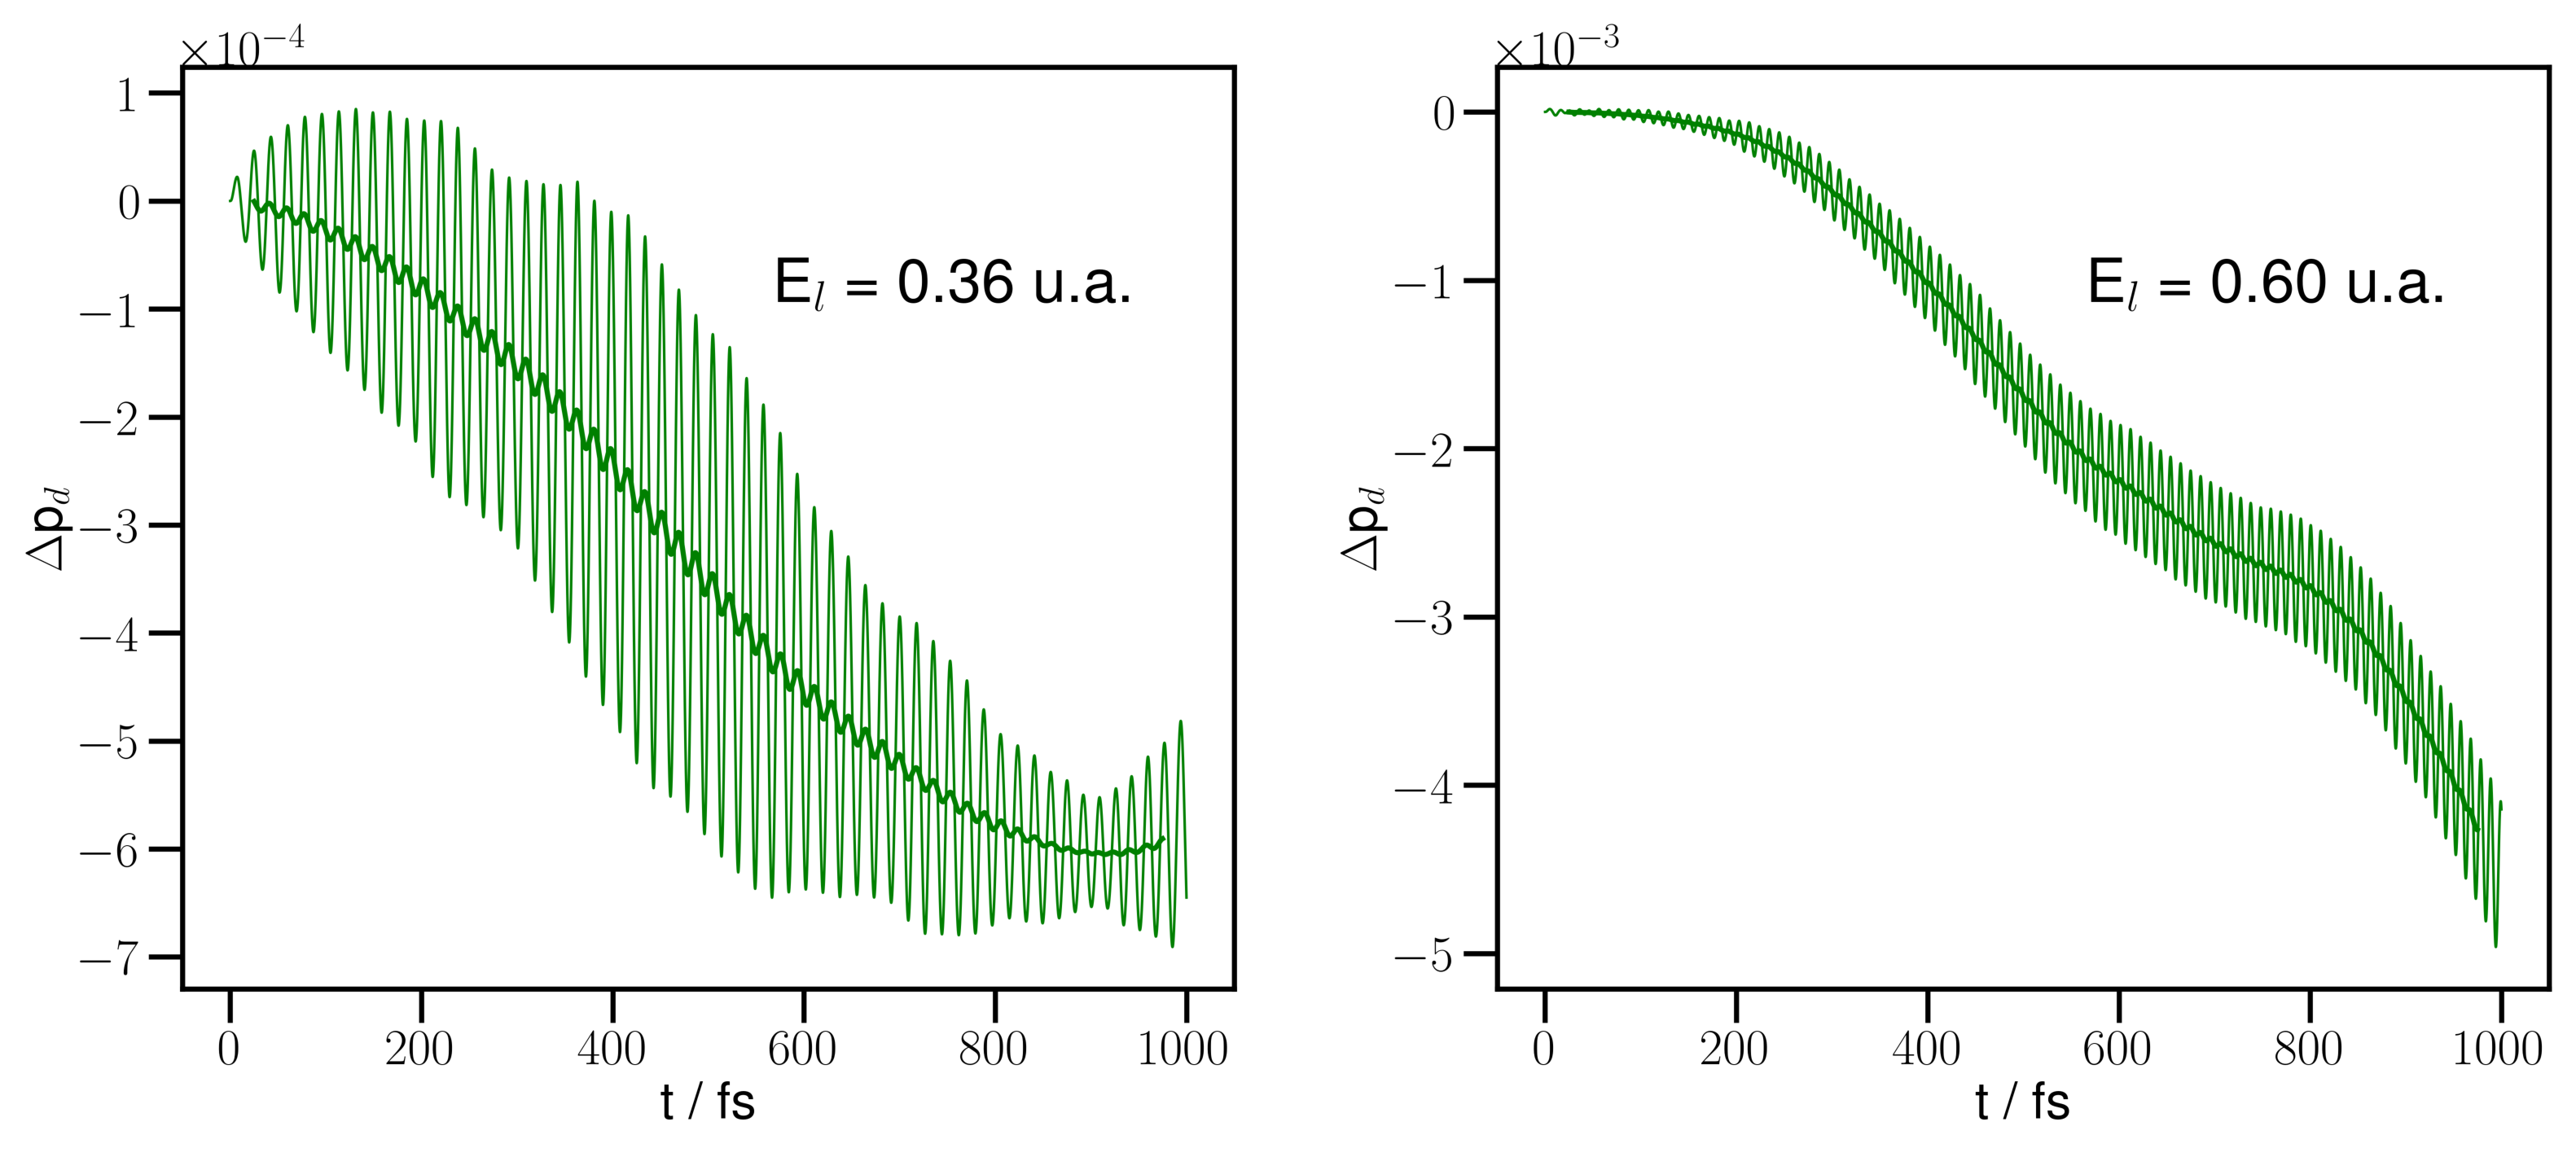
\includegraphics[height=4cm]{cap3/figs/acople_bajo.eps}
 \caption{$\Delta p_d$ en función del tiempo aplicando un campo electromagnético con energı́a $0.36$ u.a. \textbf{(izquerda)} y $0.60$ u.a. \textbf{(derecha)} al complejo con acoplamientos bajo o $\gamma = 0.02$}
 \label{acople_chico}
\end{figure}


En complejos con acoplamientos mayores, como por ejemplo \textbf{(d)}, observamos transferencia de carga mediante el mecanismo directo al iluminar los complejos con una energía de $0.36$ u.a. o con la energía de la transición H-C. En la figura \ref{acople_alto} se observa que los valores de $\Delta p_d$ al aplicar un campo con la energía de la excitación H-C, son mayores con respecto a la transferencia que produce la iluminación con la energía de la excitación H-L. Sin embargo, esta última no es tan pequeña como para considerarla despreciable. Podemos decir entonces que en sistemas donde el acoplamiento es grande, los dos mecanismos, tanto directo como indirecto contribuyen en la transferencia de carga final. 


\begin{figure}[!htb]
 \centering
 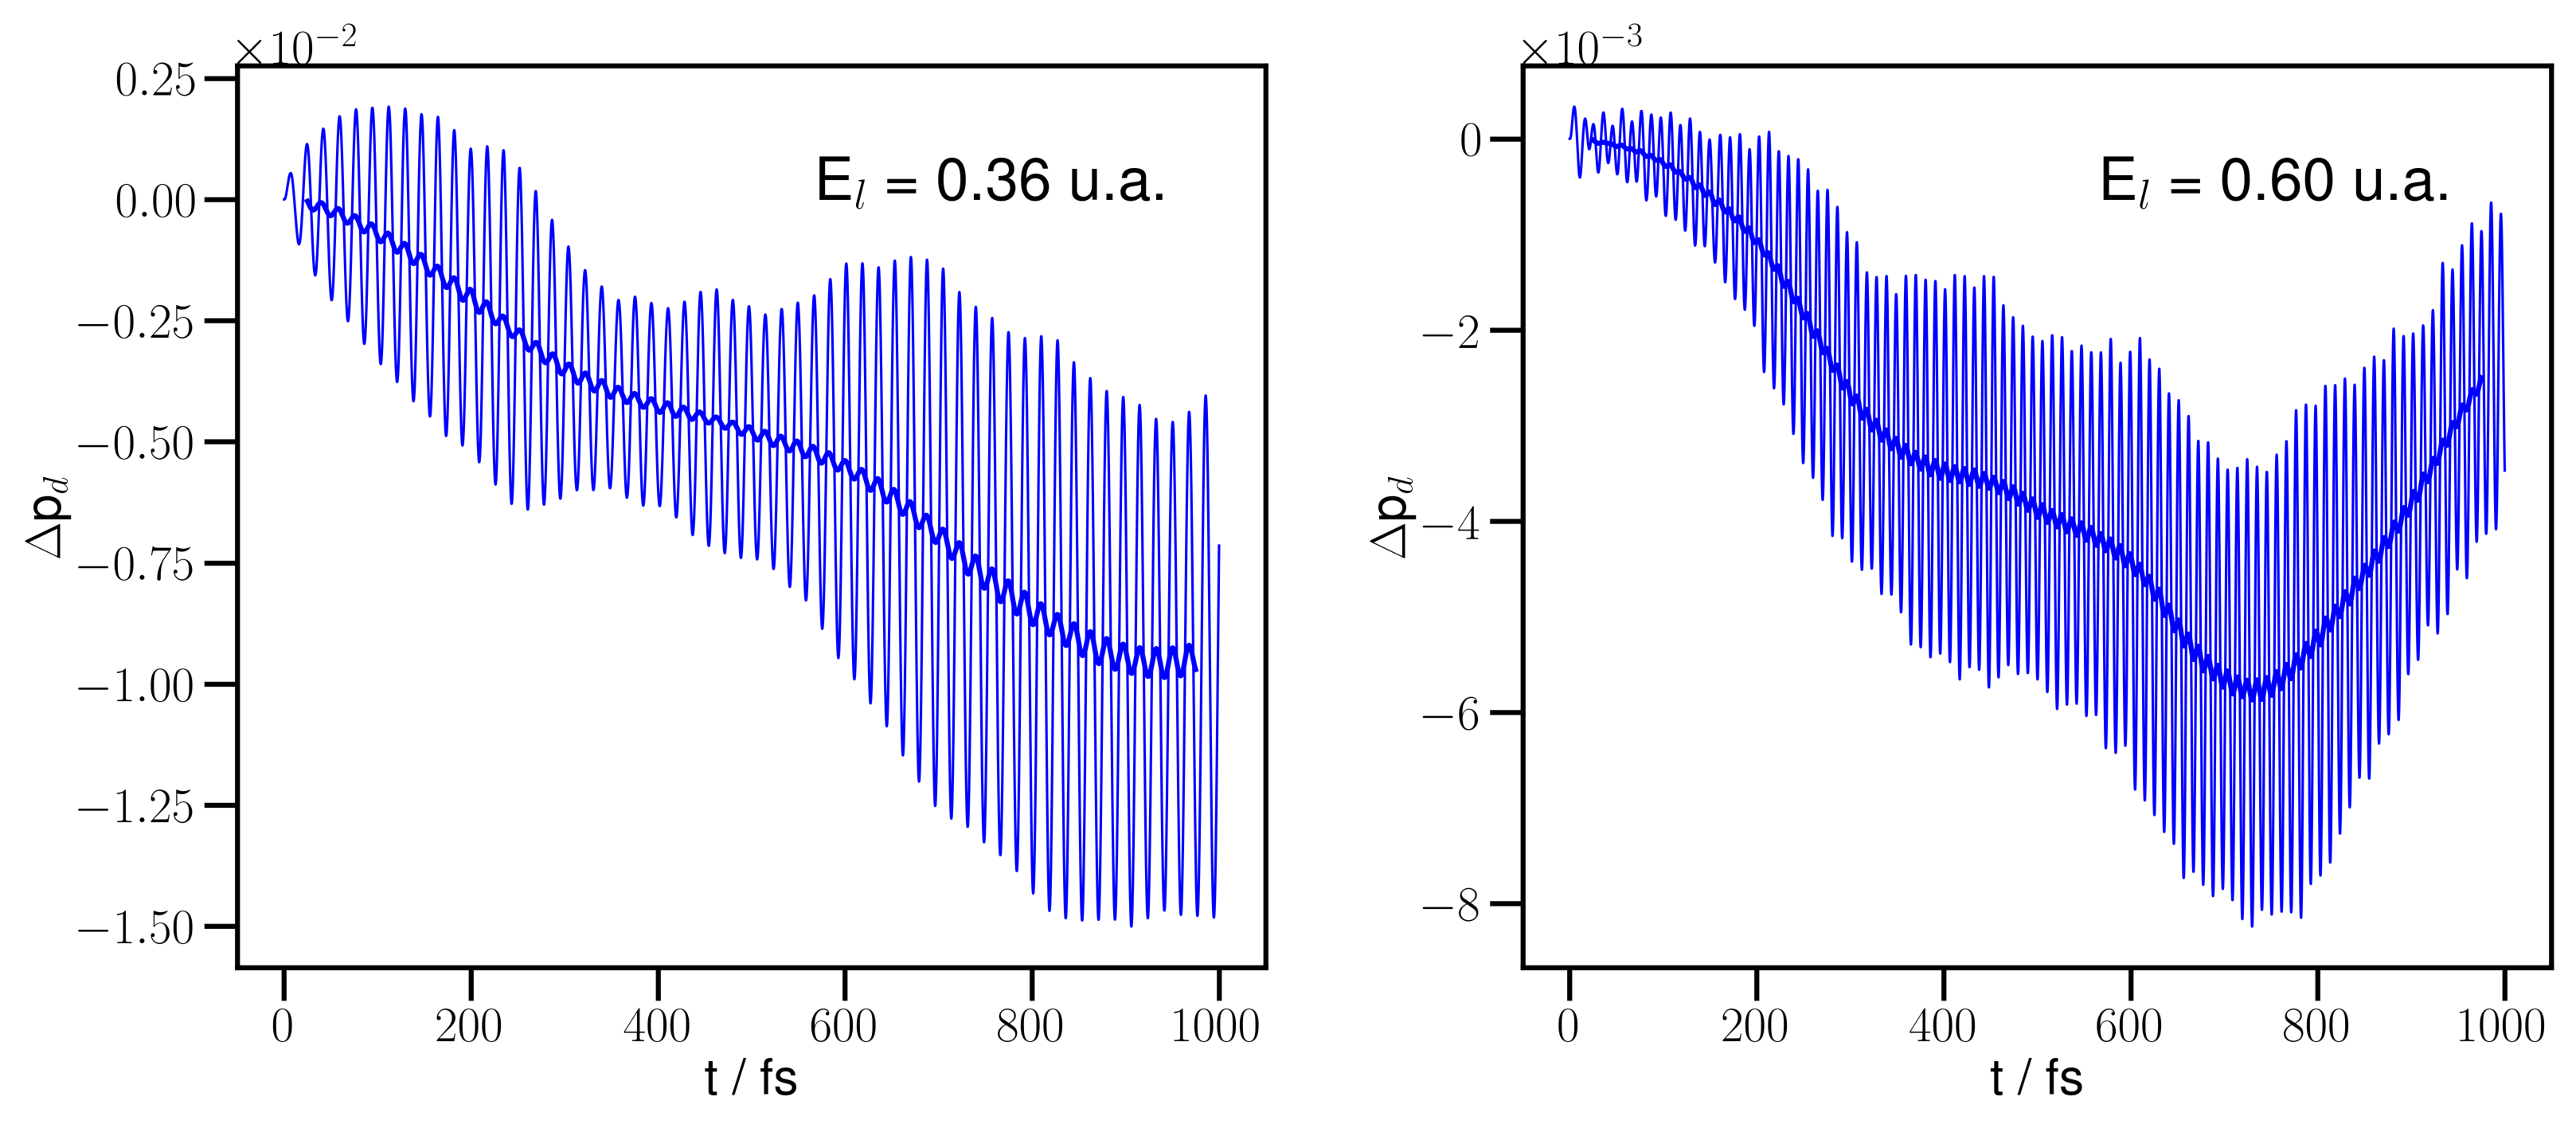
\includegraphics[height=4cm]{cap3/figs/acople_alto.eps}
 \caption{$\Delta p_d$ en función del tiempo aplicando un campo electromagnético con energı́a $0.36$ u.a. \textbf{(izquerda)} y $0.60$ u.a. \textbf{(derecha)} al complejo con acoplamientos bajo o $\gamma = 0.1$}
 \label{acople_alto}
\end{figure}
 
En última instancia consideramos complejos con las mismas constantes de acoplamiento utilizadas anteriormente, es decir, $\gamma = 0$, $\gamma = 0.02$, $\gamma = 0.05$ y $\gamma = 0.1$ pero esta vez con $\epsilon=-0.45$ y $\mu=-0.3$ constantes, tal como muestra la figura \ref{2-h-g}. Los gráficos de $\Delta p_d$ en función del tiempo \textbf{(b)}, \textbf{(c)} y \textbf{(d)} muestran la misma $\Delta p_d$ en valor absoluto en comparación a los gráficos de la figura \ref{2-e-g}, sin embargo en este caso,la inyección electrónica se produce desde el SC a la molécula.


\begin{figure}[!htb]
 \centering
 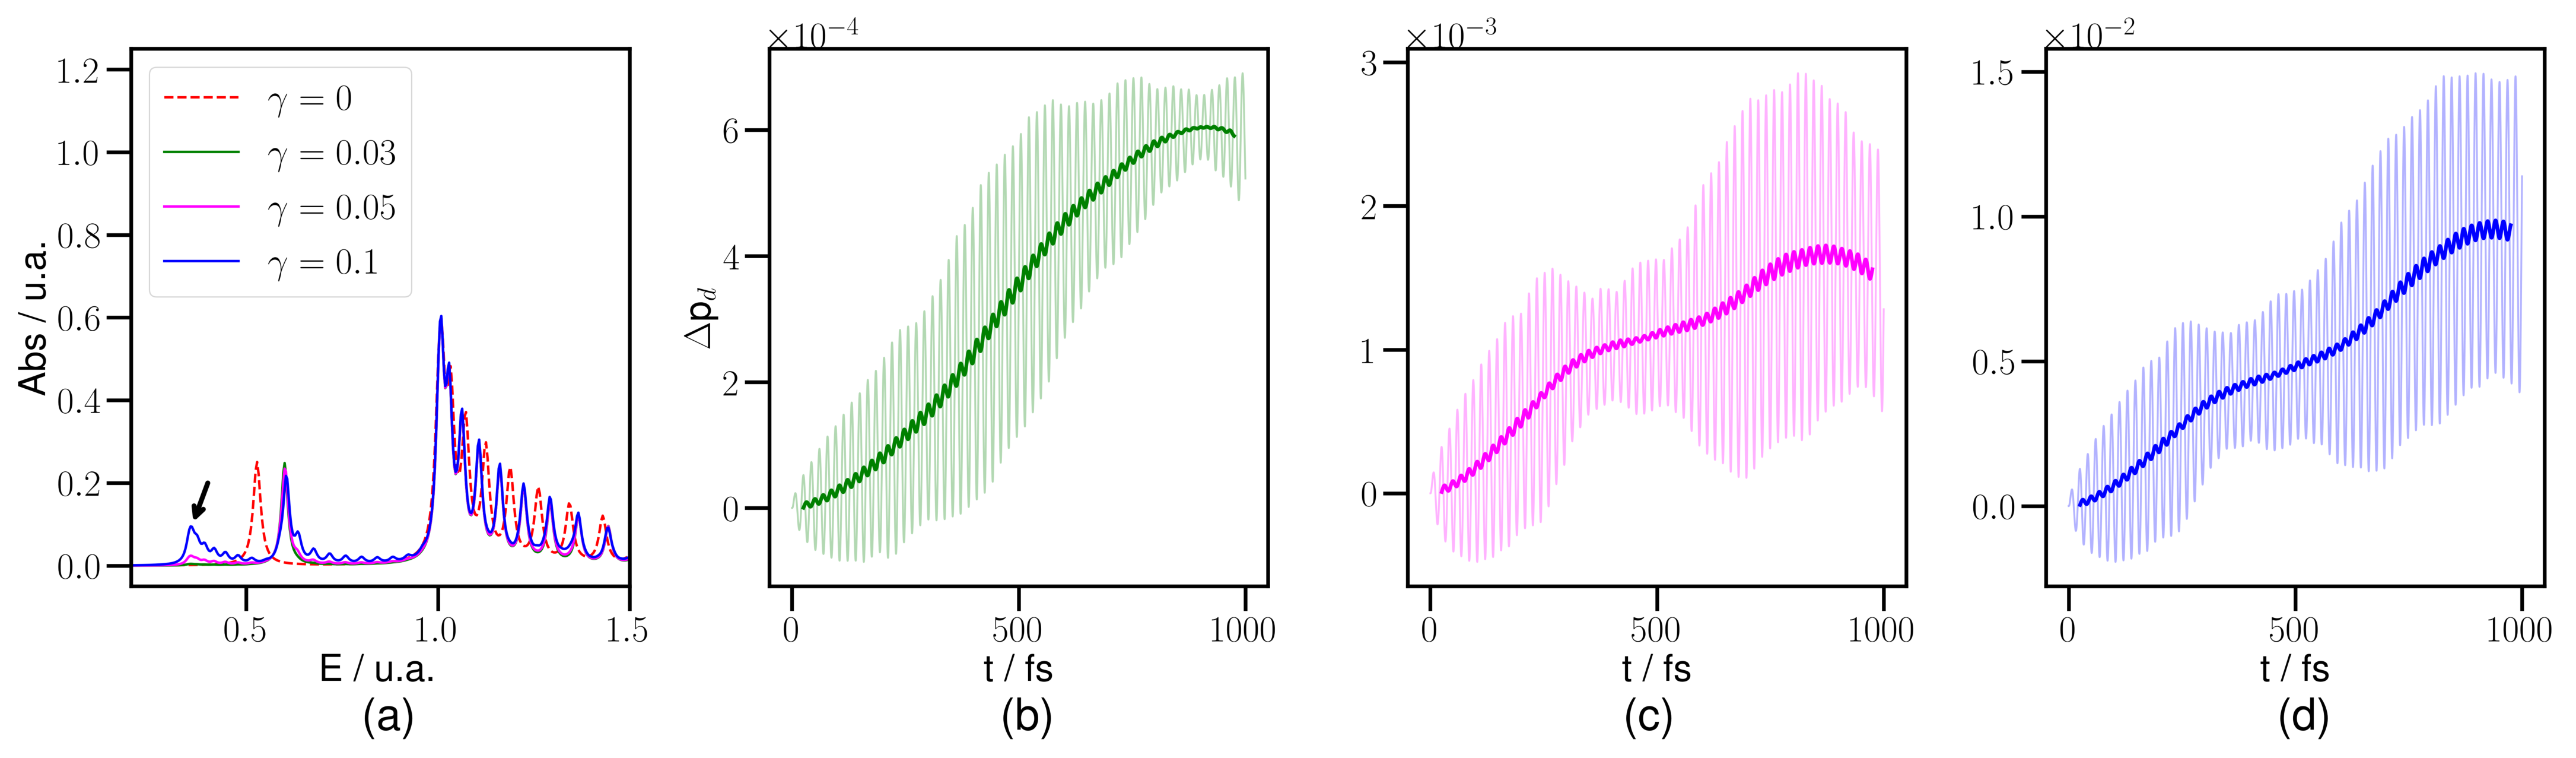
\includegraphics[height=4.3cm]{cap3/figs/fig_gamas_h.eps}
 \caption{Gráficos de \textbf{(a)} Espectro de absorción para distintos $\gamma$ y $\Delta p_d$ en función del tiempo aplicando un campo electromagnético con energı́a $0.36$ u.a. a complejos con distintos acoplamientos: \textbf{(b)} $\gamma = 0.02$, \textbf{(c)} $\gamma = 0.05$ y \textbf{(d)} $\gamma = 0.1$ utilizando $\epsilon=-0.45$ y $\mu=-0.3$ como parámetros fijos.}
 \label{2-h-g}
\end{figure}

\newpage


\section{Conclusiones}

 Los resultados obtenidos a lo largo del capítulo demuestran la efectividad del modelo para describir la dinámica electrónica del sistema molécula-SC bajo irradiación láser. Los cálculos para la DOS representan bien las BC y BV del SC separadas por un GAP y los orbitales H-L de la diatómica. Los espectros de absorción presentan claramente, en todos los casos, una banda que corresponde al SC con  una energía que comienza en 1 u.a. (energía del GAP) y un pico debido a la transición H-L. Cuando hay acoplamiento entre el anillo y la molécula aparece una nueva banda debido a nuevas transiciones posibles entre el SC y la molécula diatómica.  
 
 Cuando $\epsilon$ toma valores positivos, los orbitales de la diatómica se encuentran más cerca de la BC y por ende las transiciones menos energéticas son las que ocurren desde el HOMO a la BC. En este caso, la transferencia es electrónica. Cuando $\epsilon$ toma valores negativos, los orbitales de la diatómica se encuentran mas cerca de la BV y las transiciones menos energéticas son las transiciones que ocurren desde la BV al HOMO. En este caso la transferencia es de huecos ya que se genera una carga positiva en la BV. 
  
 Al variar la constante de acoplamiento se observó que cuando $\gamma$ es pequeña predomina el mecanismo de transferencia de carga indirecta y cuando $\gamma$ es grande predomina el mecanismo directo. Este comportamiento concuerda con lo observado anteriormente en el grupo, lo cual es otro indicio de que el modelo aunque sea simple representa bien el sistema DSSC y los procesos que ocurren en la misma.




 

  %\input{cap4/cap4}
  %\chapter{Transferencia de carga en complejos nw de ZnO wurtzita + CAT.}
%\chapter{Fotodopaje de nw ZnO wurtzita con catecol}

El óxido de zinc (ZnO) es un material SC, compuesto por elementos de los grupos II-VI, de GAP amplio y directo ($3.37$ eV a temperatura ambiente) \cite{Strehlow1973}. En los últimos años ha generado un gran interés en la comunidad científica debido al gran número de aplicaciones prácticas que abarcan desde la pintura, la fotocatálisis hasta la medicina \cite{Djurisic2006,Mishra2017}. Las propiedades físicas del ZnO y su amplio GAP acoplado a la alta energía de enlace de excitones (60 meV) \cite{Ozgur2005} hace que sea un material adecuado para aplicaciones optoelectrónicas \cite{Janisch2005}, de esta manera, las nanoestructuras de ZnO también se emplean en el campo de la producción de energía fotovoltaica.

El ZnO puede cristalizar en estructura sal de roca, cúbica (blenda de zinc) o hexagonal (wurzita) (ver figura \ref{cristales_zno}), siendo esta última la más estable termodinámicamente en condiciones ambientales. Es un SC tipo n nativo debido a la desviación en la estequiometría que se origina a partir de las vacancias de oxígeno (V$_O$) y los átomos de zinc intersticial (Zn$_i$) \cite{Ozgur2005}. Los trabajos científicos de Look \emph{et al.} \cite{Look1998,Look1999} sostienen que el Zn$_i$ es el donante superficial nativo dominante en ZnO y otros proponen que la conductividad tipo n de las películas de ZnO dopadas involuntariamente se debe solo al hidrógeno \cite{Strzhemechny2004}. Esta suposición tiene sentido ya que el hidrógeno siempre está presente en todos los métodos de crecimiento y puede difundirse fácilmente en el ZnO en grandes cantidades debido a su gran movilidad. Cálculos de primeros principios basados en el DFT también sostienen que el hidrógeno incorporado involuntariamente actúa como una fuente de conductividad y se comporta como un donante superficial en ZnO \cite{VanDeWalle2000}. El dopaje de tipo n de ZnO es relativamente fácil en comparación con el dopaje de tipo p. Los elementos Al, Ga e In del grupo III como elementos sustitutos de Zn y los elementos Cl e I del grupo VII como elementos sustitutos de O pueden utilizarse como dopantes de tipo n \cite{Kato2002}. Sin embargo, es difícil alcanzar un buen dopaje tipo p en el ZnO debido a varias causas, una es la autocompensación causada por defectos intrínsecos, es decir, en un intento de dopar el material tipo p, ciertos defectos nativos que actúan como donantes pueden formarse espontáneamente y compensar deliberadamente aceptores \cite{Fan2013}, otra posibilidad es la baja solubilidad del dopante en el material. 


\begin{figure}[!htb]
\centering
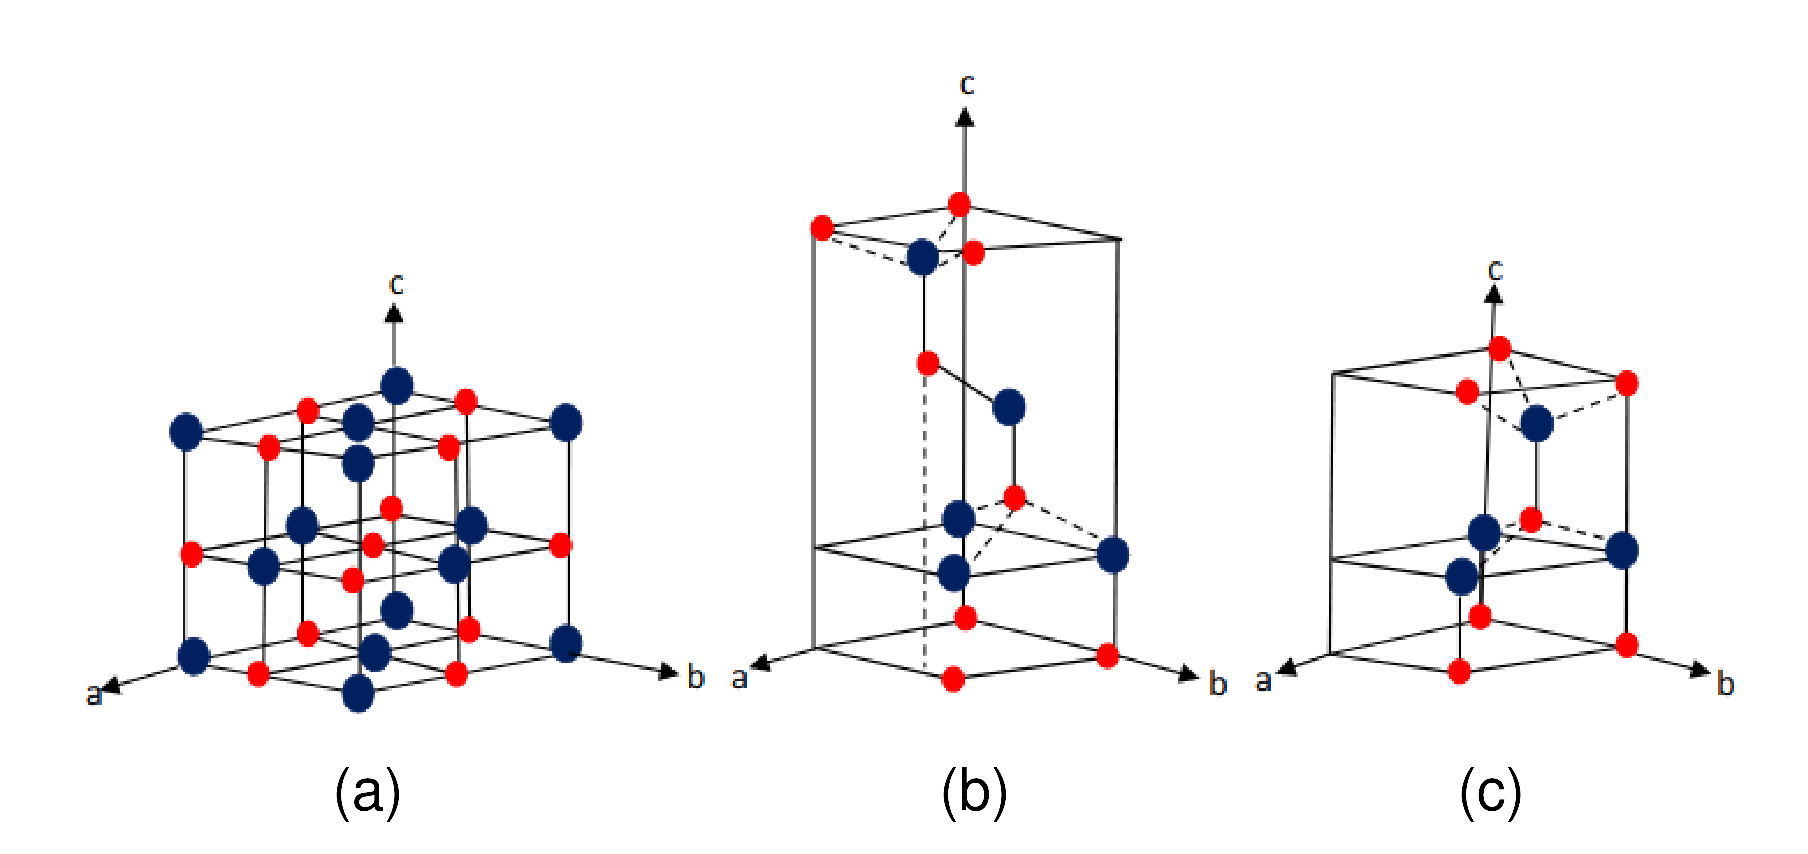
\includegraphics[height=5cm]{cap5/fig/est_zno.eps}
\caption{Estructuras cristalinas de ZnO: (a) sal de roca, (b) blenda de zinc y (c) wurtzita. Los círculos rojos y azules representan a los iones de zinc y oxígeno, respectivamente.} 
\label{cristales_zno}
\end{figure}

ZnO es un material amigable con el medio ambiente, en consecuencia, existe un interés en estudiar el ZnO en forma de polvos, monocristales, películas delgadas o nanoestructuras. Se han reportado una gran variedad de morfologías nanoestructuradas de ZnO como nanowires, nanorods, tetrapods, nanoribbons/belts, clusters \cite{Mishra2017, Huang2001_a,Huang2001_b, Liu2003,Shabani2020, Chauhan2018, Yan2003, Singh2020}, etc., como muestra la figura \ref{nanoestructuras_zno}. Los nanowires (nw) son SC unidimensionales que han captado la atención debido a sus propiedades físicas derivadas del confinamiento cuántico, como el transporte cuántico electrónico y la recombinación radiativa mejorada de portadores. Estas nanoestructuras son los sistemas ideales para estudiar los mecanismos de transporte en sistemas unidimensionales, que son beneficiosos no solo para comprender los fenómenos fundamentales en sistemas de baja dimensión sino también para desarrollar nanodispositivos de nueva generación con alto rendimiento \cite{Ozgur2005}. Los nw son prometedores en amplias aplicaciones y son los bloques de construcción fundamentales para la fabricación de nano-láseres de longitud de onda corta, transistores de efecto de campo, sensores ultrasensibles de gas de tamaño nanométrico, nanoresonadores, transductores, emisores de campo, etc. \cite{Huang2001_a,Wang2004_a, Wang2004_b,Heo2004}. De acuerdo a la literatura \cite{Ghosh2020,Nayeri2013,Peng2011,Baxter2005}, los nw de ZnO wurtzita también son buenos candidatos para fotoelectrodos en las DSSC, no solo por las ventajas de la morfología, al proporcionar una ruta directa a los electrones, sino también por las propiedades que provienen del material como la alta movilidad electrónica con respecto a otros SC, crecimiento anisotrópico, la facilidad de cristalización, etc. \cite{Tiwana2011,Law2005} que también aportan al buen funcionamiento de la celda.

\begin{figure}[!htb]
\centering
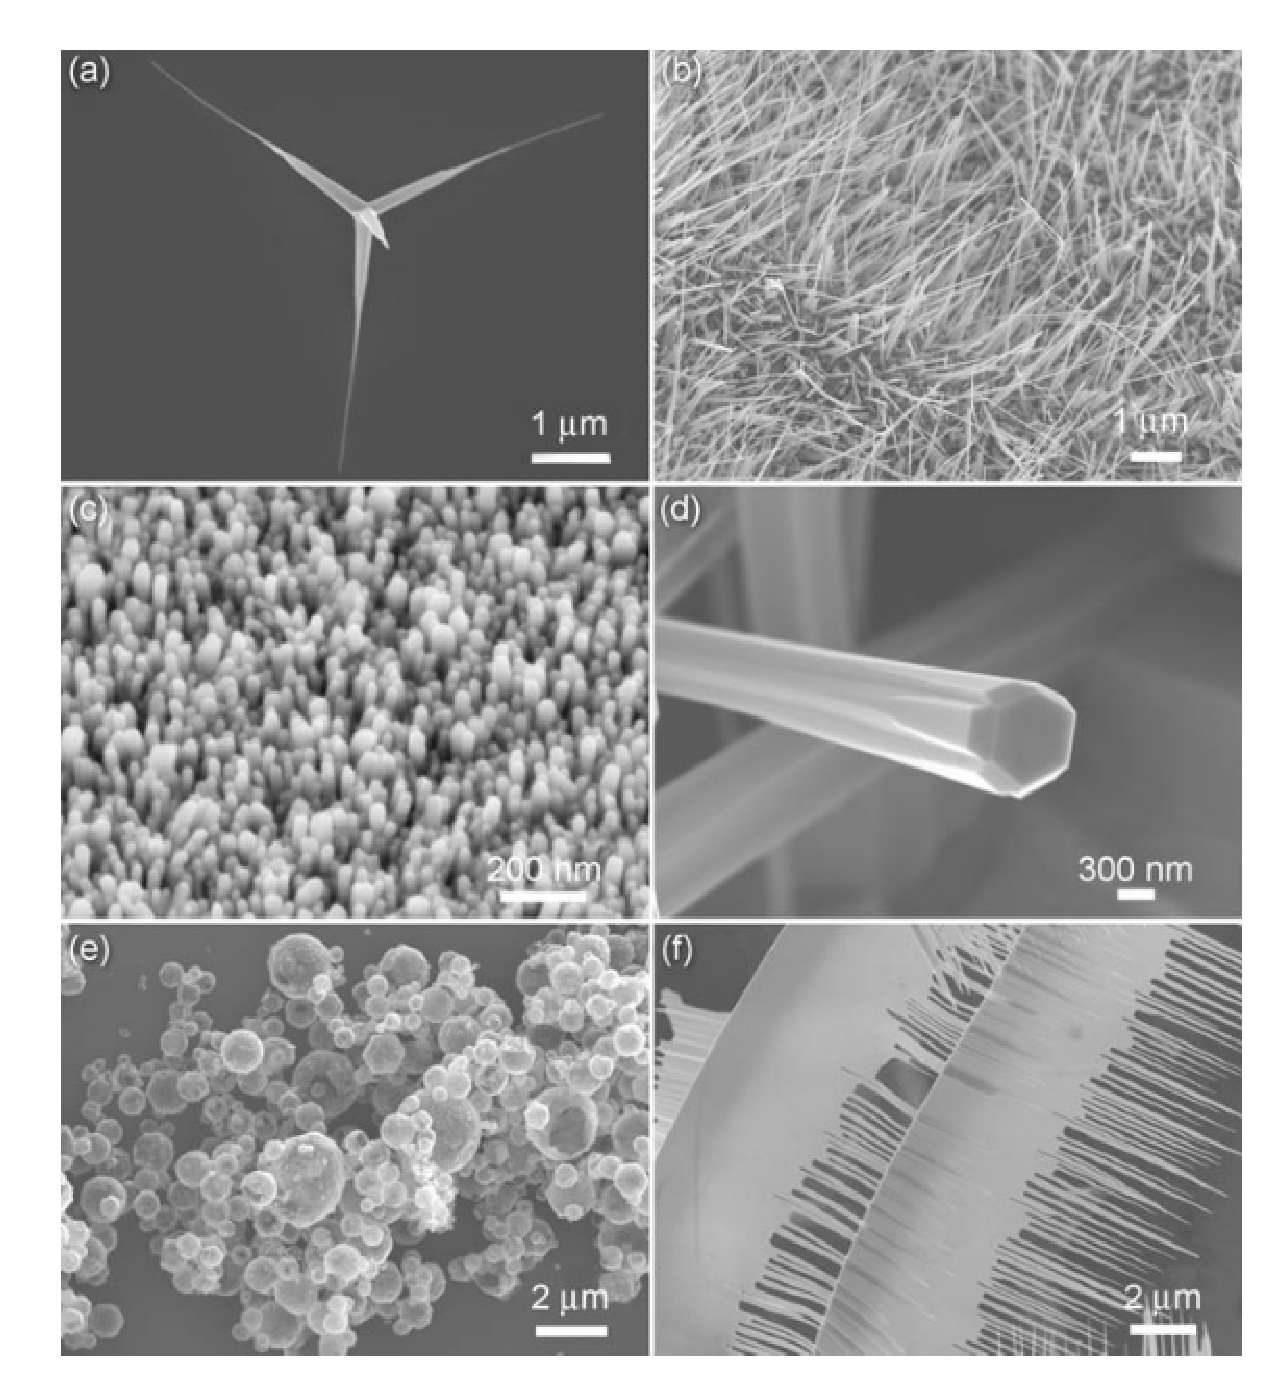
\includegraphics[height=9cm]{cap5/fig/nanoestructuras_zno.eps}
\caption{ (a-f) Imágenes representativas de microscopía electrónica de barrido de diversas morfologías de nanoestructura de ZnO. Extraído de \cite{Djurisic2006}}
\label{nanoestructuras_zno}
\end{figure}

Como se mencionó en el capítulo 4, las DSSC se clasifican en tipo I y tipo II  dependiendo de la vía de inyección que tomen los electrones desde el colorante absorbido al SC (ver figura \ref{tipos_dssc}). En las celdas tipo II, los electrones se inyectan no sólo por el camino indirecto o tipo I, sino también por la vía directa o de “un sólo paso” desde el estado fundamental del sensibilizador a la BC del SC mediante la excitación fotoinducida de las bandas de transferencia de carga colorante-SC ({\bf C-S}) como se ilustra en el esquema (b) de la figura \ref{tipos_dssc}. 

\begin{figure}[!htb]
\centering
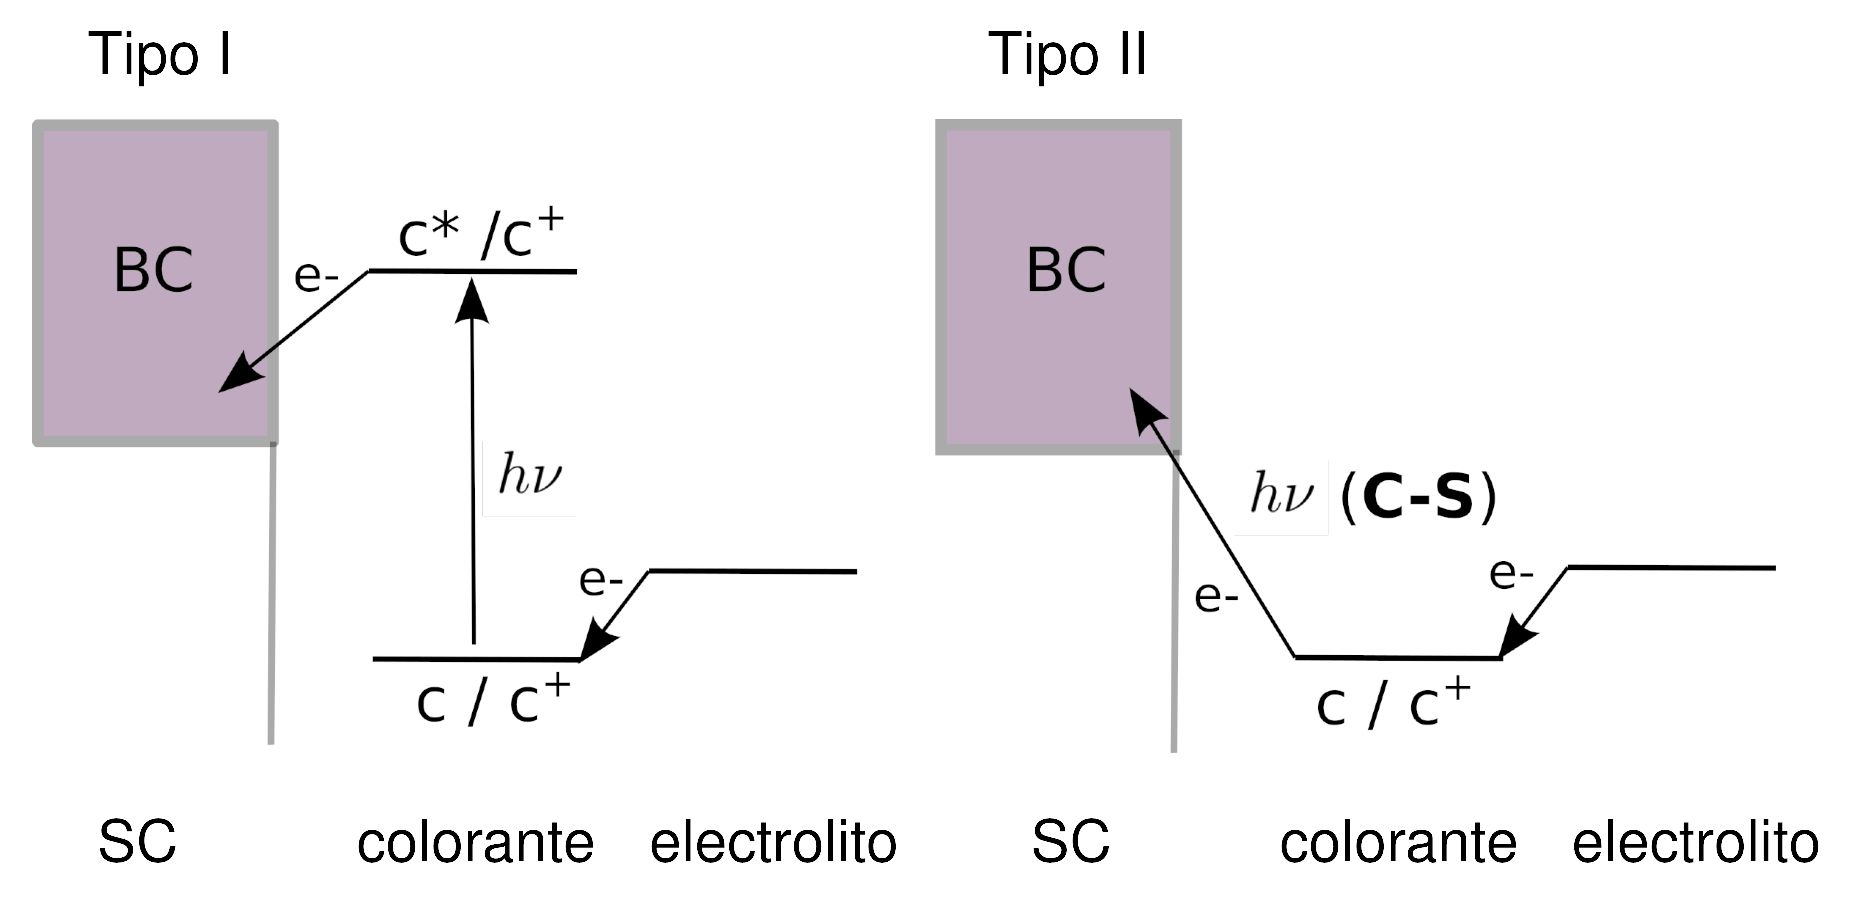
\includegraphics[height=7cm]{cap5/fig/tipo1_tipo2.eps}
\caption{Diferentes vías de inyección electrónica en sistemas colorante-SC desde la molécula al SC}
\label{tipos_dssc}
\end{figure}

De trabajos anteriores se conoce que las moléculas que tienen enodiol en su estructura se unen a la superficie del TiO$_2$ a través de la quelación de los iones de Ti de la superficie con los grupos enodiol, dando lugar a bandas de C-S generalmente muy intensas \cite{Tae2005}. En particular, el CAT y sus derivados como la dopamina, fluorona, numerosos pigmentos naturales como el rojo de bromopirogalol y las antocianinas \cite{Sinopoli2017, Persson2000, Dimitrijevic2003, Frei1990, Ramakrishna2001} son ejemplos típicos de DSSC de tipo II ya que tienen restos de CAT en su estructura y en consecuencia muestran fuertes bandas C-S en la región visible al unirse al TiO$_2$. También se ha demostrado que la fotoexcitación de las bandas C-S da lugar a una inyección directa de electrones de los colorantes al TiO$_2$ muy rápida, menor a $100$ fs \cite{Wang2003,Huber2000}, de acuerdo con la teoría de transferencia de carga de Mulliken \cite{Mulliken1952}.

A pesar de que los colorantes tipo II puedan inyectar electrones al TiO$_2$ por dos caminos y la eficiencia de inyección de electrones de la vía directa, en principio debería ser 1, no se han empleado rigurosamente como sensibilizadores para DSSC debido a que los valores de eficiencia cuántica externa ({\bf EQE}) son menores a las eficiencias de las DSSC sensibilizadas con colorantes tipo I. Una de las razones por las que la EQE de la vía directa son tan bajas radica en el hecho de que las velocidades de transferencia electrónica desde el TiO$_2$ reducido a la molécula oxidada, es decir la recombinación de carga, son mayores para la vía directa (en el orden de los picosegundos \cite{Ramakrishna2001,Wang2003, Huber2000}) que para la indirecta. En este sentido, el desarrollo de métodos para aumentar la eficiencia de la vía directa no es solo un gran desafío en sí mismo sino que también de gran interés desde el punto de vista académico y práctico.

En el capítulo previo, se estudió el complejo CAT-NP TiO$_2$ no solo porque es un colorante que opera por la vía directa sino también porque cuando se adsorbe sobre la superficie de TiO$_2$, el umbral de absorción óptica se reduce significativamente en energía. Como muestra la figura \ref{specs_cat}, la cual expone los espectros de absorción óptica del catecol aislado obtenido experimentalmente \cite{Dewar1958} y calculado con dftb+, el máximo de absorción de la banda de mínima energía se encuentra en la zona del UV. Ambos espectros son similares cualitativamente, teniendo en cuenta que en el espectro experimental se utilizó un solvente orgánico en la medición mientras que en el cálculo teórico el CAT se encuentra en el vacío. 

En este capítulo se realizaron estudios teóricos a nivel DFTB y TD-DFTB de la estructura electrónica y propiedades ópticas de los complejos {\bf CAT-nw ZnO} debido a las particularidades que presentan el CAT y el nw desde el punto de vista electrónico aunque a priori no sea un sistema que garantice una buena eficiencia en una DSSC al tratar con un sensibilizador tipo II. 

\begin{figure}[!htb]
\centering
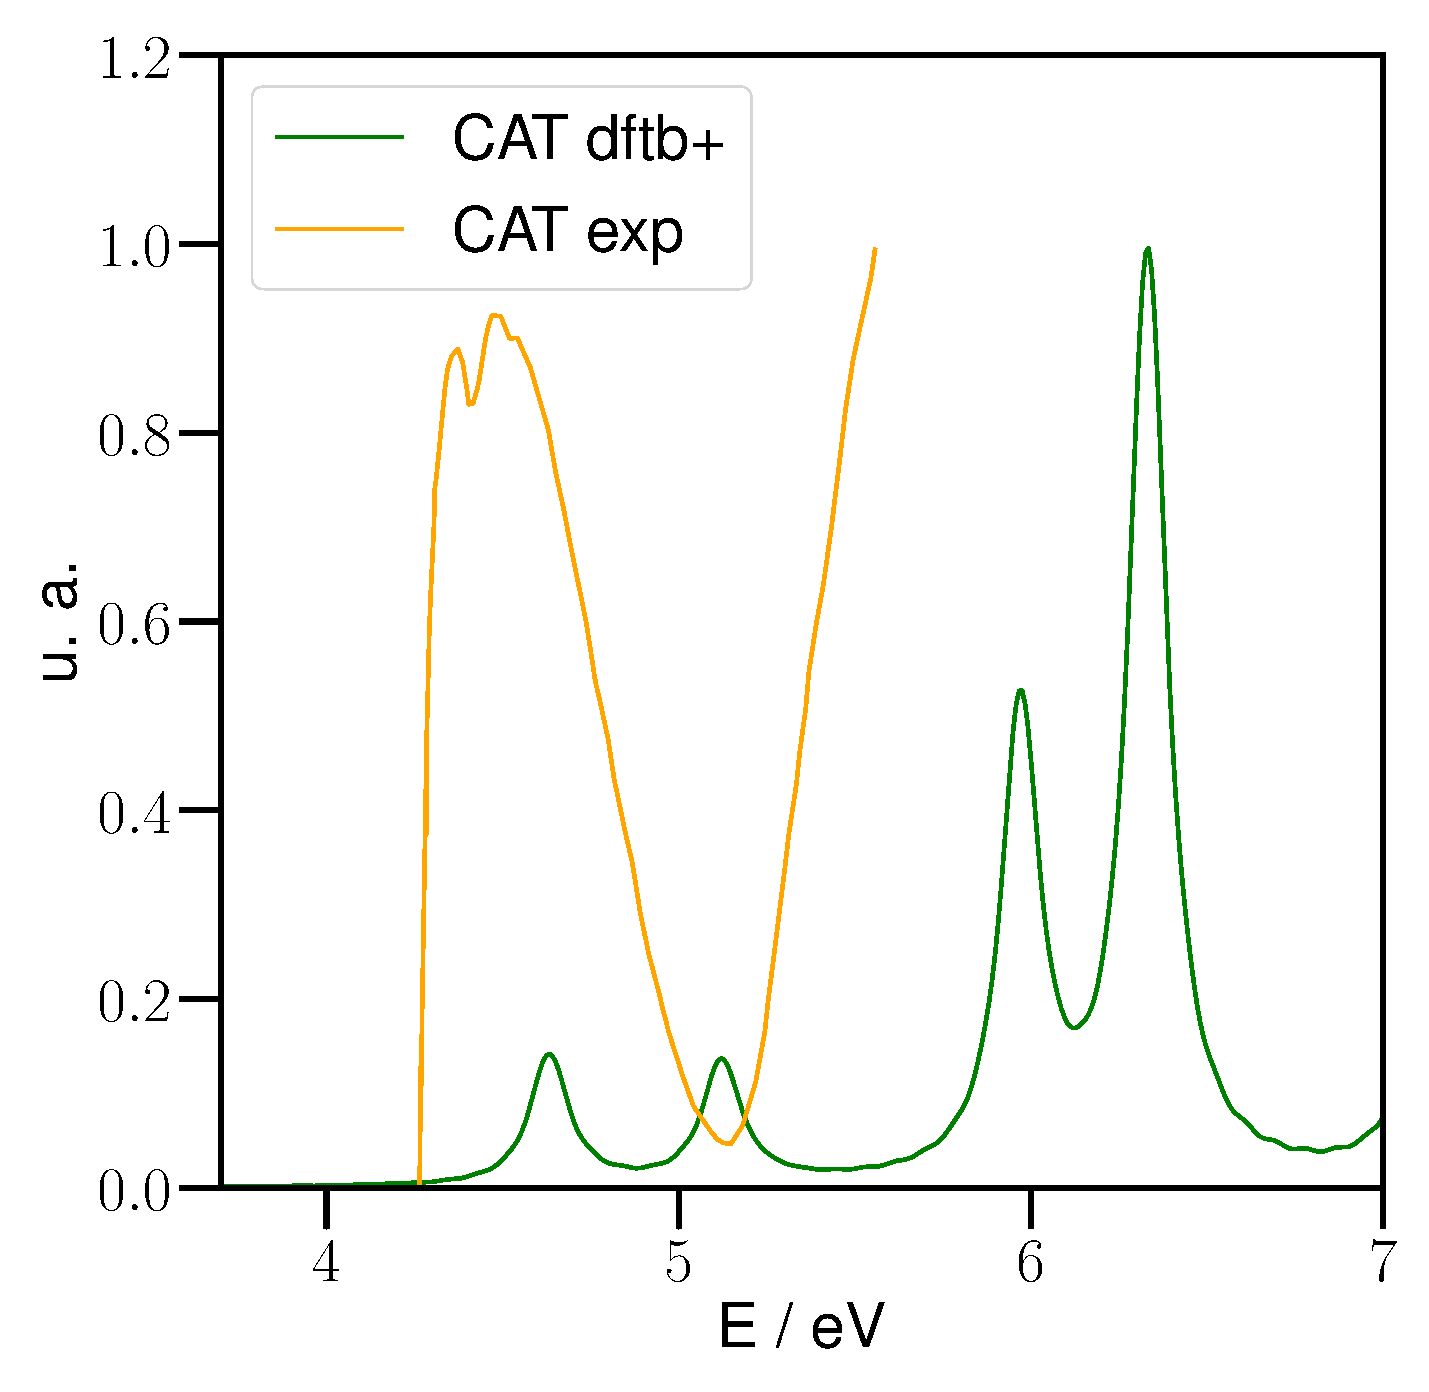
\includegraphics[height=9cm]{cap5/fig/specs_cat.eps}
\caption{Espectros de absorción óptica de CAT aislado obtenidos experimentalmente (naranja) y teóricamente con dftb+ (verde)}
\label{specs_cat}
\end{figure}

\section{Detalles computacionales}

Los parámetros utilizados para calcular los espectros de absorción y las dinámicas electrónicas son los mismos que se utilizaron en el capítulo 4, es decir: paso de tiempo $0.005$ fs, cantidad de pasos 20000 e intensidad del campo $0.0001$ $\frac{V}{\AA}$ y $0.01$ $\frac{V}{\AA}$, respectivamente. La diferencia radica en el estudio de la dinámica electrónica del sistema analizado, ya que en este capítulo se realizó aplicando perturbaciones sinusoidales sintonizadas con la energía de los máximos de absorción en el rango (0-4) eV.

\section{Estructura electrónica en equilibrio}

\subsection{Energía de adsorción}


\begin{figure}[!htb]
\centering
\includegraphics[height=4.5cm]{cap5/fig/estructuras_flecha.eps}
\caption{Sistemas de estudio CAT+nw con diferentes cubrimientos. Con colores más intensos se muestra la celda unidad (C$_1$) y las superceldas (el resto de los complejos)}
\label{estructuras}
\end{figure}


El primer objetivo del capítulo fue estudiar los distintos cubrimientos de colorante (CAT) en el nw (ver figura \ref{estructuras}) y analizar el efecto que produce en la estructura electrónica en el equilibrio. Para realizar el estudio se utilizaron 6 sistemas CAT-nw: {\bf C$_1$}, {\bf C$_2$}, {\bf C$_3$}, {\bf C$_4$}, {\bf C$_5$} y {\bf C$_6$}, los cuales son el resultado de la adsorción monodentada del colorante en su forma disociada a la superficie del nw. En trabajos anteriores del grupo \cite{Negre2012} hemos encontrado que aunque la unión bidentada disociativa del CAT es energéticamente preferida, para este modelo de TB, esta forma es inestable y por esta razón, hemos considerado sólo la forma monodentada. En todos los casos, para mantener al sistema neutro, el protón disociado fue agregado a un O del nw, adyacente al sitio de anclaje. Para lograr los distintos cubrimientos se utilizaron superceldas con nw de distintos tamaños: C$_1$ se construyó sólo con la celda unidad de nw wurtzita la cual consta de 48 átomos y un diámetro de $9.8 \r{A}$. En el sistema C$_2$, en cambio, se apilaron dos celdas unidad de nw en el eje z para formar la supercelda, en C$_3$ tres celdas unidad y así para todos los sistemas. A medida que aumenta el largo del nw en las superceldas, las moléculas de CAT están a una distancia mayor, de esta manera, en C$_1$ las moléculas entre celdas contiguas se encuentran lo más cerca posible y por lo tanto es el caso de máximo cubrimiento mientras que en C$_6$ se encuentran más lejos en distancia con respecto a otros complejos siendo este caso el de mínimo cubrimiento. Un punto importante a destacar es el hecho de que las moléculas de CAT se encuentran en forma CIS, es decir, dispuestas unas arriba de otras, ya que es más estable para dftb+ esta conformación y por ello es la usaremos a lo largo de todo el capítulo.

Para caracterizar la unión entre el colorante y la superficie del nw se calcularon las energías de adsorción (E$_{ad}$) para los seis complejos planteados. Antes de realizar estos cálculos es necesario aclarar que los colorantes fueron optimizados con dftb+ antes de la adsorción al nw y despues de que esto ocurra en conjunto con unidades de ZnO adyacentes al punto de unión y además las estructuras de los nw se obtuvieron utilizando dinámica molecular a 300 K con el programa LAMMPS. 

\begin{figure}[!htb]
\centering
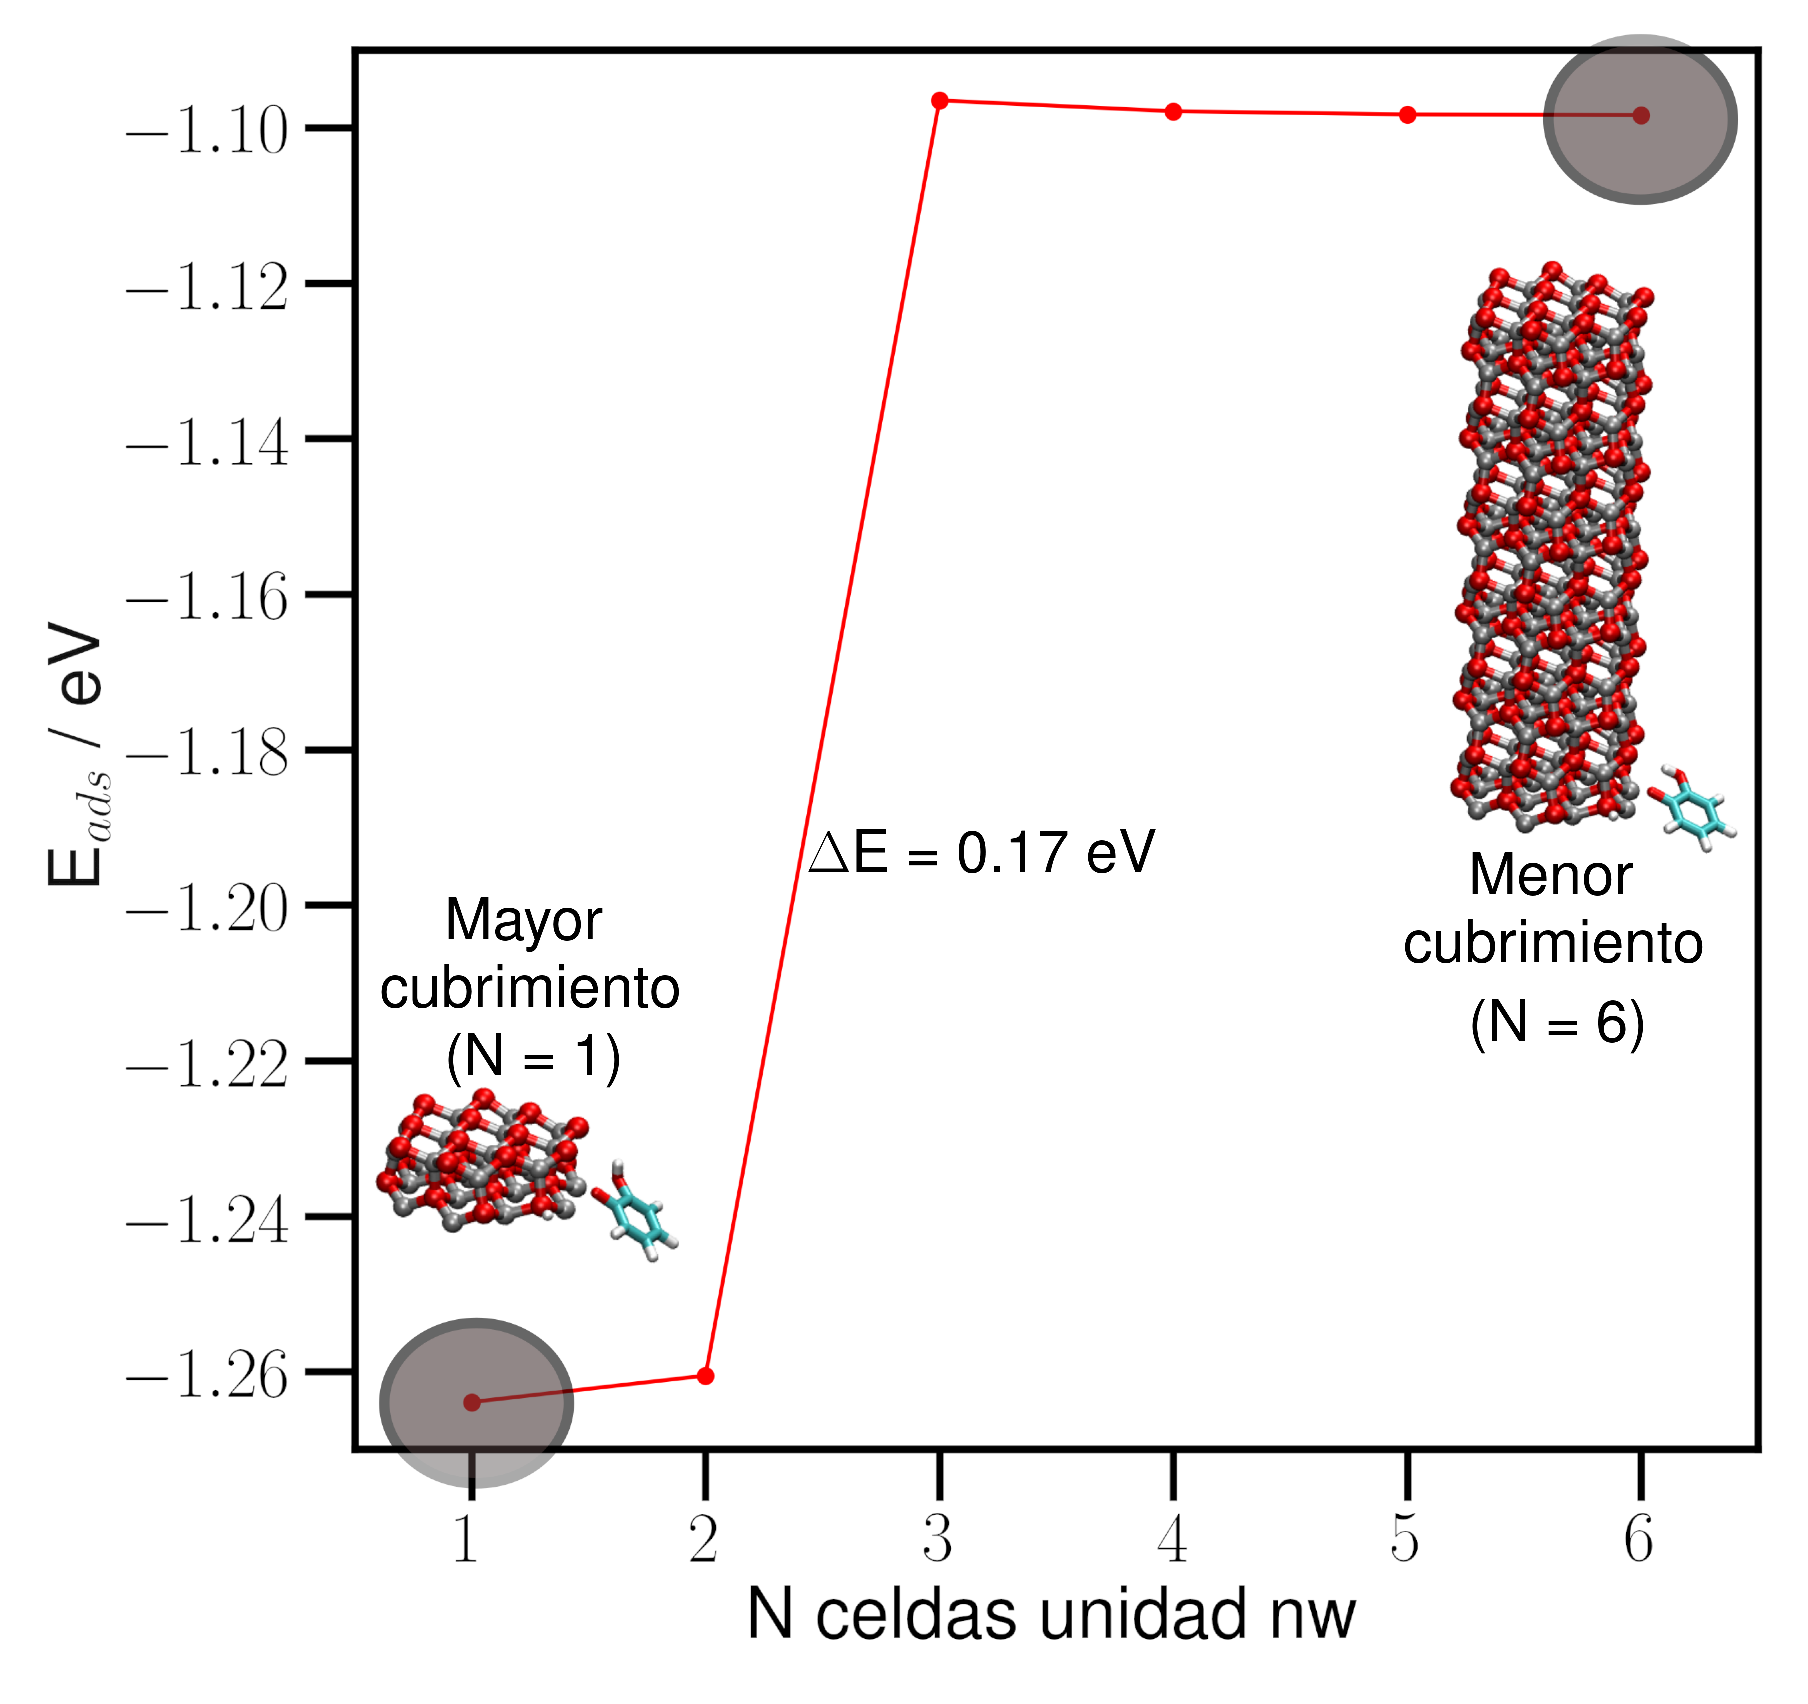
\includegraphics[height=11cm]{cap5/fig/e_ad_F.eps}
\caption{Energía de adsorción para los 6 sistemas estudiados en función de los distintos largos de superceldas de nw en relación a la celda unidad.}
\label{ead}
\end{figure}


La E$_{ad}$ se obtuvo de acuerdo a la siguiente ecuación:

\begin{equation}
 E_{ad} = E_{T(nw + CAT)} - E_{T(nw)} - E_{T(CAT)}
\end{equation}

donde E$_{T(nw + CAT)}$) es la energía total del complejo nw + CAT, E$_{T(nw)}$ la energía total del nw de ZnO y E$_{T(CAT)}$ de la molécula CAT. 


La figura \ref{ead} es un gráfico de E$_{ad}$ en función de N celdas unidad de nw, es decir, la cantidad de celdas unidad apiladas en el eje z: C$_1$ se correponde con N=1 y C$_2$ con N=2, etc. Se observan valores negativos de E$_{ad}$ entre $-1.1$ eV y $-1.3$ eV aproximadamente, reflejando una unión fuerte entre el adsorbato (CAT) y el adsorbente (nw). Estos resultados indican una quimisorción ya que las moléculas adsorbidas reaccionan químicamente con la superficie generando la formación de un enlace entre el CAT y el nw. A su vez, N=1 y N=2 (C$_1$ y C$_2$, respectivamente) muestran una E$_{ad}$ relativamente mayor (en valor absoluto) con respecto a los otros sistemas, la cual denota una estabilidad adicional en estos complejos que no se observa en otros. La diferencia de energía entre N=2 y N=3 es de $0.17$ eV y en principio se puede atribuír a distancias cortas entre catecoles. Las fuerzas de Van der Waals entre moléculas sólo justifican el complejo C$_1$ ya que en C$_2$ los CAT se encuentran a distancias lo suficientemente largas como para que esta interacción no tenga efecto. La causa por la cuál ocurre esta estabilización es la estudiaremos a lo largo del capítulo.

%A su vez, N=1 y N=2 (C$_1$ y C$_2$) muestran una E$_{ad}$ mayor en valor absoluto con respecto a los otros sistemas y se observa un delta de energía de $0.17$ eV entre N=2 y N=3 que corresponde a valores entre $13 - 15\%$ de la E$_{ad}$. Entonces, el hecho de que en C$_1$ y C$_2$ los catecoles se encuentren a distancias menores con respecto a los demás sistemas, otorga a los mismos una estabilidad adicional que no se observa en otros casos. 


%Esta estabilización puede deberse a {\bf (a)} interacciones tipo Van der Waals entre catecoles, {\bf (b)} diferencias conformacionales, {\bf (c)} interacciones entre los OM. La hipótesis {\bf (a)} sólo justificaría el complejo C$_1$ ya que en C$_2$ los catecoles se escuentran a distancias largas para considerar este tipo de interacciones. La hipótesis {\bf (b)} se pondrá a prueba a lo largo del capítulo. 

\subsection{Estructura de bandas}

El método de TB o combinación lineal de orbitales atómicos ({\bf CLOA}) es un método semiempírico que se utiliza principalmente para calcular la estructura de bandas y los estados de Bloch de una sola partícula de un material. El método de TB semi-empírico es simple y computacionalmente muy rápido y por lo tanto, tiende a usarse en cálculos de sistemas muy grandes, con más de unos pocos miles de átomos en la celda unidad.
 

\subsubsection{Cálculo de estructura de bandas dentro del formalismo TB}

%Para sistemas que contienen hasta unos cientos o miles de átomos, podemos utilizar la DFT para encontrar la densidad del estado fundamental real y la energía del estado fundamental del sistema que interactúa sin calcular explícitamente la función de onda de muchos electrones. En un cálculo de este tipo obtenemos energías aproximadas de una sola partícula que, en la práctica, a menudo dan una aproximación razonable a la estructura de bandas real del cristal. En sistemas aún más grandes, con alrededor de $10.000$ o más átomos, ya no podemos usar cálculos de DFT autoconsistentes para tener en cuenta la interacción completa. 

Cuando se calcula la estructura de bandas y un conjunto de estados de una sola partícula aproximados utlizando el método de TB, se intenta incluir los efectos de la interacción de una manera semiempírica, utilizando parámetros que podemos ajustar y que coincidan con el experimento. El punto de partida de todos los enfoques semiempíricos es la física. En los metales, por ejemplo, los electrones son casi libres, por lo que podemos tratar los estados de una sola partícula en términos de ondas planas. También podemos adoptar un enfoque diferente y asumir que los estados en un cristal son combinaciones de funciones de onda de átomos aislados, lo cual es más probable que sea el caso de los aislantes o semiconductores. A continuación, resolveremos la ecuación de Schr\" odinger de una sola partícula para los estados en un cristal expandiendo los estados de Bloch en términos de una combinación lineal de orbitales atómicos \cite{Roy2015}. 

En un cristal, definimos el hamiltoniano de una sola partícula como  

\begin{equation}
 H = H_{at} + \Delta U,
\end{equation}


donde $H_{at}$ es el hamiltoniano de un solo átomo y $\Delta U$ comprende todas las diferencias entre el verdadero potencial en el cristal y el potencial de un átomo aislado. Suponemos $\Delta U \rightarrow 0$ en el centro de cada átomo del cristal. Los estados de una sola partícula en el cristal son entonces $\Psi_{n {\bf k}}({\bf r})$, donde 

\begin{equation}
H \, \Psi_{n {\bf k}}({\bf r}) = E_{n {\bf k}}  \Psi_{n {\bf k}}({\bf r}),
\end{equation}

el índice de banda está etiquetado por n, y {\bf k} es un vector de onda de la primera zona de Brillouin. Las {\bf funciones de onda atómicas}, $\phi_{i}({\bf r})$, son estados propios de $H_{at}$,

\begin{equation}
H_{at} \, \phi_{i}({\bf r}) = \epsilon_{i}  \phi_{i}({\bf r}),
\end{equation}

donde $\epsilon_{i}$ es la energía del nivel de energía i en un átomo aislado. Estas funciones de onda decaen rápidamente alejándose de $r = 0$ y, por lo tanto, la integral de solapamiento, $\gamma (|{\bf R}|) = \int \phi^* ({\bf r})\, H\, \phi ({\bf r} + {\bf R})  \, d{\bf r}$, es pequeña entre funciones de onda ubicadas en sitios atómicos separados (${\bf R} \neq 0$) en el cristal (ver figura \ref{tb_orb}). 

%\begin{equation}
%\int{\phi_{i}^*({\bf r})\phi_{j}({\bf r} + {\bf R} ) \, d{\bf r}} = \left\lbrace
%\begin{array}{ll}
%1 & \textup{si} \hspace{0.2cm} i=j \hspace{0.2cm} y \hspace{0.2cm} {\bf R} = 0  \\
%0 & \textup{de otra manera}
%\end{array}
%\right.
%\label{eq:solapamiento}
%\end{equation}

\vspace{1cm}

\begin{figure}[!htb]
\centering
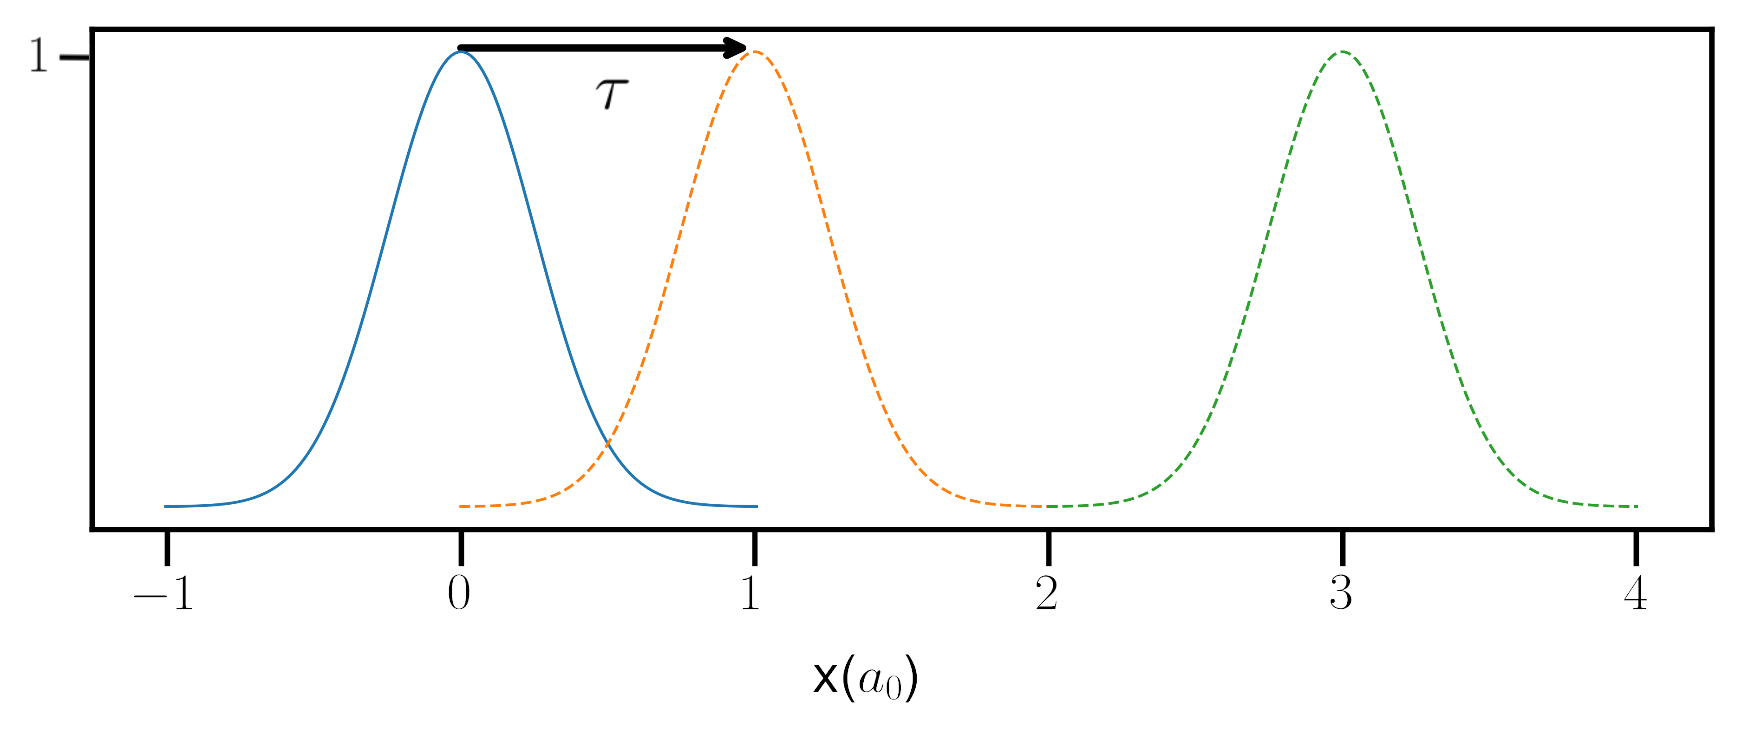
\includegraphics[height=6cm]{cap5/fig/gauss_final.eps}
\caption{Esquema de los orbitales atómicos en un cristal 1D con átomos separados por $a_0$. Los vectores de traslación son ${\bf R} = 0$,$\pm a_0{\bf i}$, $\pm 2a_0{\bf i}$, $\pm 3a_0{\bf i}$,$...$, donde ${\bf i}$ es un vector unitario en la dirección $x$. Se muestra en el diagrama uno de los vectores vecinos más cercanos, $\tau = a_0{\bf i}$ y las líneas de puntos verticales denotan los bordes de la celda unidad que contiene un solo átomo. El gráfico azul muestra un orbital atómico centrado en un átomo en $r=0$, mientras que los gráficos con líneas discontinuas muestran orbitales centrados en $r+\tau$ y $r+3\tau$. Aquí asumimos que la integral de superposición,$\int \phi^* ({\bf r})\, H\, \phi ({\bf r} + {\bf R})  \, d{\bf r}$, es sólo significativa cuando $|{\bf R}|$ está cerca de $|\tau|$.}
\label{tb_orb}
\end{figure}


\newpage

Los estados de una sola partícula, $\Psi_{n {\bf k}}({\bf r})$, deben obedecer el {\bf teorema de Bloch}, 

\begin{equation}
\displaystyle \Psi_{n {\bf k}}({\bf r} + {\bf R}) =  e^{i {\bf k}.{\bf R}} \Psi_{n {\bf k}}({\bf r}), 
\end{equation}

donde ${\bf R}$ es un vector de traslación espacial real del cristal. Un solo orbital atómico no satisface el teorema de Bloch, pero podemos plantear fácilmente una CLOA que sí lo haga,  

\begin{equation}
\displaystyle \Psi_{n {\bf k}}({\bf r}) = \frac{1}{\sqrt{N}} \sum_{{\bf R}} e^{i {\bf k}.{\bf R}} \phi_n ({\bf r}-{\bf R}), 
\end{equation}

donde hay N sitios de red en el cristal y el factor $\frac{1}{\sqrt{N}}$ asegura que el estado de Bloch esté normalizado. 

\begin{itemize}
 \item Banda s en un cristal 1D
\end{itemize}

Imaginemos un cristal con vectores de traslación {\bf R}, que tiene un átomo en la celda unidad, y donde solo los orbitales atómicos s $\phi_{s}({\bf r})$ contribuyen a los estados del cristal. En el caso de un {\bf cristal 1D}, los vectores de traslación son ${\bf R} = na_0{\bf i}$ donde n es un número entero, $a_0$ es la separación atómica e {\bf i} es un vector unitario en la dirección x. En este caso, hay dos vectores de traslación vecinos más cercanos $\tau = \pm a_0 {\bf i}$. Entonces solo hay 1 banda (n = 1) y solo hay un estado de Bloch que podemos construir,

\begin{equation}
\displaystyle \Psi_{{\bf k}}({\bf r}) = \frac{1}{\sqrt{N}} \sum_{{\bf R}} e^{i {\bf k}.{\bf R}} \phi_s ({\bf r}-{\bf R}), 
\label{eq:psi_single_s_band}
\end{equation}

En este caso simple podemos encontrar la {\bf relación de dispersión} (la relación entre la energía y el vector de onda) simplemente calculando el valor esperado o de expectación de la energía, 

\begin{align}
E({\bf k}) &= \int \Psi^*_{{\bf k}} ({\bf r})\, H\, \Psi_{\bf k} ({\bf r})  \, d{\bf r} \label{exp_e_paso1} \\
& = \frac{1}{\sqrt{N}} \sum_{{\bf R}} \sum_{{\bf R'}} e^{i {\bf k}.({\bf R'} -{\bf R}) } \int \phi^*_s ({\bf r} - {\bf R})\, H\, \phi_s ({\bf r} - {\bf R'})  \, d{\bf r} \label{exp_e_paso2} \\ 
&= \frac{1}{\sqrt{N}} \sum_{{\bf R}} \sum_{{\bf R'}} e^{i {\bf k}.({\bf R'} - {\bf R}) } \int \phi^*_s (x)\, H\, \phi_s (x - ({\bf R} - {\bf R'}))  \, d{\bf x} \label{exp_e_paso3}\\
&= \sum_{{\bf R''}} e^{i {\bf k}.{\bf R''}} \int \phi^*_s (x)\, H\, \phi_s (x - ({\bf R} - {\bf R'}))  \, d{\bf x} \label{exp_e_paso4}\\
&= \epsilon_s + \sum_{\tau} e^{i {\bf k}.\tau} \, \gamma(|\tau|) \label{exp_e_paso5}
\end{align}

donde las integrales están sobre todo el espacio. La expresión final (ec. \ref{exp_e_paso5}) para el valor de expectación se obtuvo a partir de la ec. \ref{exp_e_paso1} siguiendo los siguientes pasos:

\begin{enumerate}
 \item Sustitución de $\Psi_{{\bf k}}({\bf r})$ de la ec. \ref{eq:psi_single_s_band} en la ec. \ref{exp_e_paso1} 
 \item Cambio de variables de {\bf r} a x = {\bf r} - {\bf R} en la ec. \ref{exp_e_paso3} 
 \item Reemplazo de {\bf R'}-{\bf R} con el vector de traslación {\bf R''} = {\bf R'}-{\bf R} en la ec. \ref{exp_e_paso4} debido a que la suma sobre {\bf R'} tiene en cuenta todos los vectores de traslación, obtendremos el mismo resultado al sumar sobre otro vector de traslación. Una vez que hacemos esto, reconocemos que la suma de {\bf R} simplemente da un factor de N, un término para cada uno de los N valores posibles de R. 
 \item Ahora en la ec. \ref{exp_e_paso5} podemos separar diferentes términos en la suma de {\bf R''} considerando el rango de los orbitales s atómicos. En el primer término, es decir {\bf R''=0}, se observa la energía del orbital atómico $\phi_s$ en un átomo aislado, $\epsilon_s$ y para el segundo término la sumatoria sobre {\bf R''} pequeño como por ejemplo {\bf R''} = $\tau$ que es el vector de traslación entre un átomo y sus vecinos más cercanos y por último se reemplazó la integral de solapamiento, $\gamma$, con un parámetro cuyo valor coincida con el experimento.
 \end{enumerate}
  
 En un cristal 1D sabemos que $\tau = \pm a_0 {\bf i}$ y que los únicos vectores de onda significativos, {\bf k}, también deben estar en la dirección de {\bf i}, de modo que {\bf k} = k{\bf i}. Entonces, 

 \begin{align}
E({\bf k}) &= \displaystyle \epsilon_s + \gamma(a_0) (e^{ika_0} + e^{-ika_0}) \nonumber \\
           &= \epsilon_s + 2\gamma(a_0) \cos(k a_0) \label{exp_e_final}
\end{align}

La ec. \ref{exp_e_final} es la relación de dispersión para una sola banda s en un cristal 1D. Describe cómo varía la energía con el momento del cristal,{\bf ancho de banda}, y también nos dice el {\bf ancho de banda}. 

En general, un material tendrá más de un átomo en la celda unidad y las bandas tendrán contribuciones de más de un tipo de orbital. En un cristal con N$_b$ bases atómicas (y donde solo un tipo de orbital atómico contribuye a los estados de banda) podemos hacer Nb combinaciones lineales de orbitales atómicos que satisfagan el teorema de Bloch, los índices i = 1, 2,. . . ,N$_b$ etiquetan cada uno de los diferentes átomos de la base y los ${\bf R'}_i$ son vectores de traslación entre átomos de tipo $i$. Sin embargo, es muy fácil generalizar este formalismo para tratar con múltiples tipos de orbitales, todo lo que tenemos que hacer es usar el índice i para etiquetar diferentes sitios base y diferentes tipos de orbitales.

Los SC son sólidos donde los átomos constituyen una red tridimensional infinita. El solapamiento de los orbitales atómicos va más allá de los primeros vecinos, extendiéndose por toda la red; resulta entonces una configuración de estados deslocalizados muy próximos entre sí, que forman bandas de estados electrónicos permitidos. Entre las bandas, hay intervalos de energía en los cuales no hay estados electrónicos permitidos (GAP) mientras que las bandas de valencia y conducción surgen del solapamiento de los niveles atómicos de los electrones de valencia. La figura \ref{origen_bandas} es un esquema que ilustra el origen de las bandas dentro del formalismo TB. En un átomo aislado tenemos un conjunto de niveles atómicos individuales, por ejemplo, 1s, 2s, 2p, etc. En un cristal con N átomos y superposición cero entre estados atómicos tendríamos N niveles degenerados para cada estado atómico. A medida que aumenta la integral de solapamiento, estos niveles se amplían en bandas, cada una de las cuales contiene N valores diferentes de {\bf k} permitidos. 

\begin{figure}[!htb]
\centering
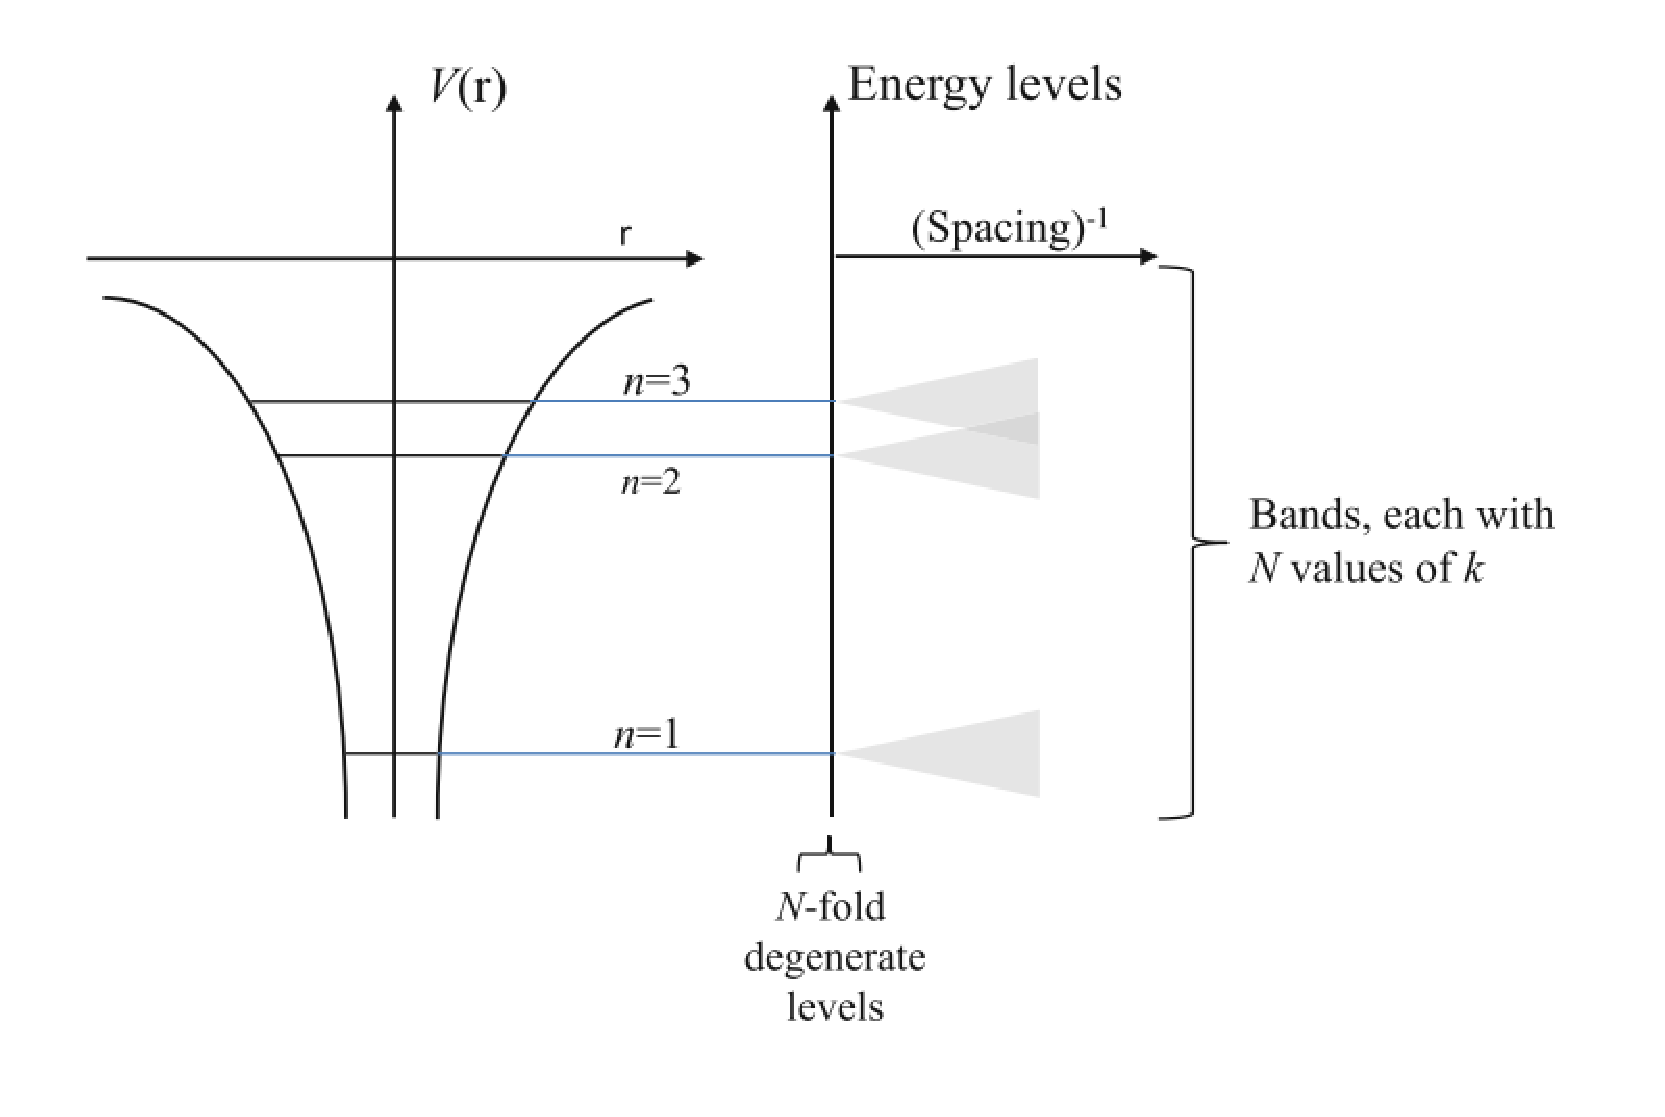
\includegraphics[height=6cm]{cap5/fig/formacion_bandas.eps}
\caption{ {\bf (Izquierda)} los niveles electrónicos no generados en un solo átomo. {\bf (Derecha)} niveles de energía para los átomos de N en un cristal, representados como una función de la integral de solapamiento o la inversa del espacio atómico. Extraído de \cite{Dresselhaus2018}}
\label{origen_bandas}
\end{figure}


\subsubsection{Cálculo de estructura de bandas en sistemas CAT-nw}

La estructura electrónica de bandas de un SC dado es fundamental para determinar su potencial utilidad. En consecuencia, un conocimiento preciso de la estructura de bandas es fundamental para desarrollar dispositivos eficientes. Dicho esto, primero calculamos con dftb+ las bandas para el SC aislado, es decir, para las 6 superceldas de ZnO wurtzita de distinta altura tal como muestra la figura \ref{bandas_nw_aislados}. En la misma se muestran los gráficos de energía en función del vector de onda {\bf k}, en particular los puntos críticos de alta simetría G y Z de la zona de brillouin (ZB) donde G es el origen. 

\begin{figure}[!htb]
\centering
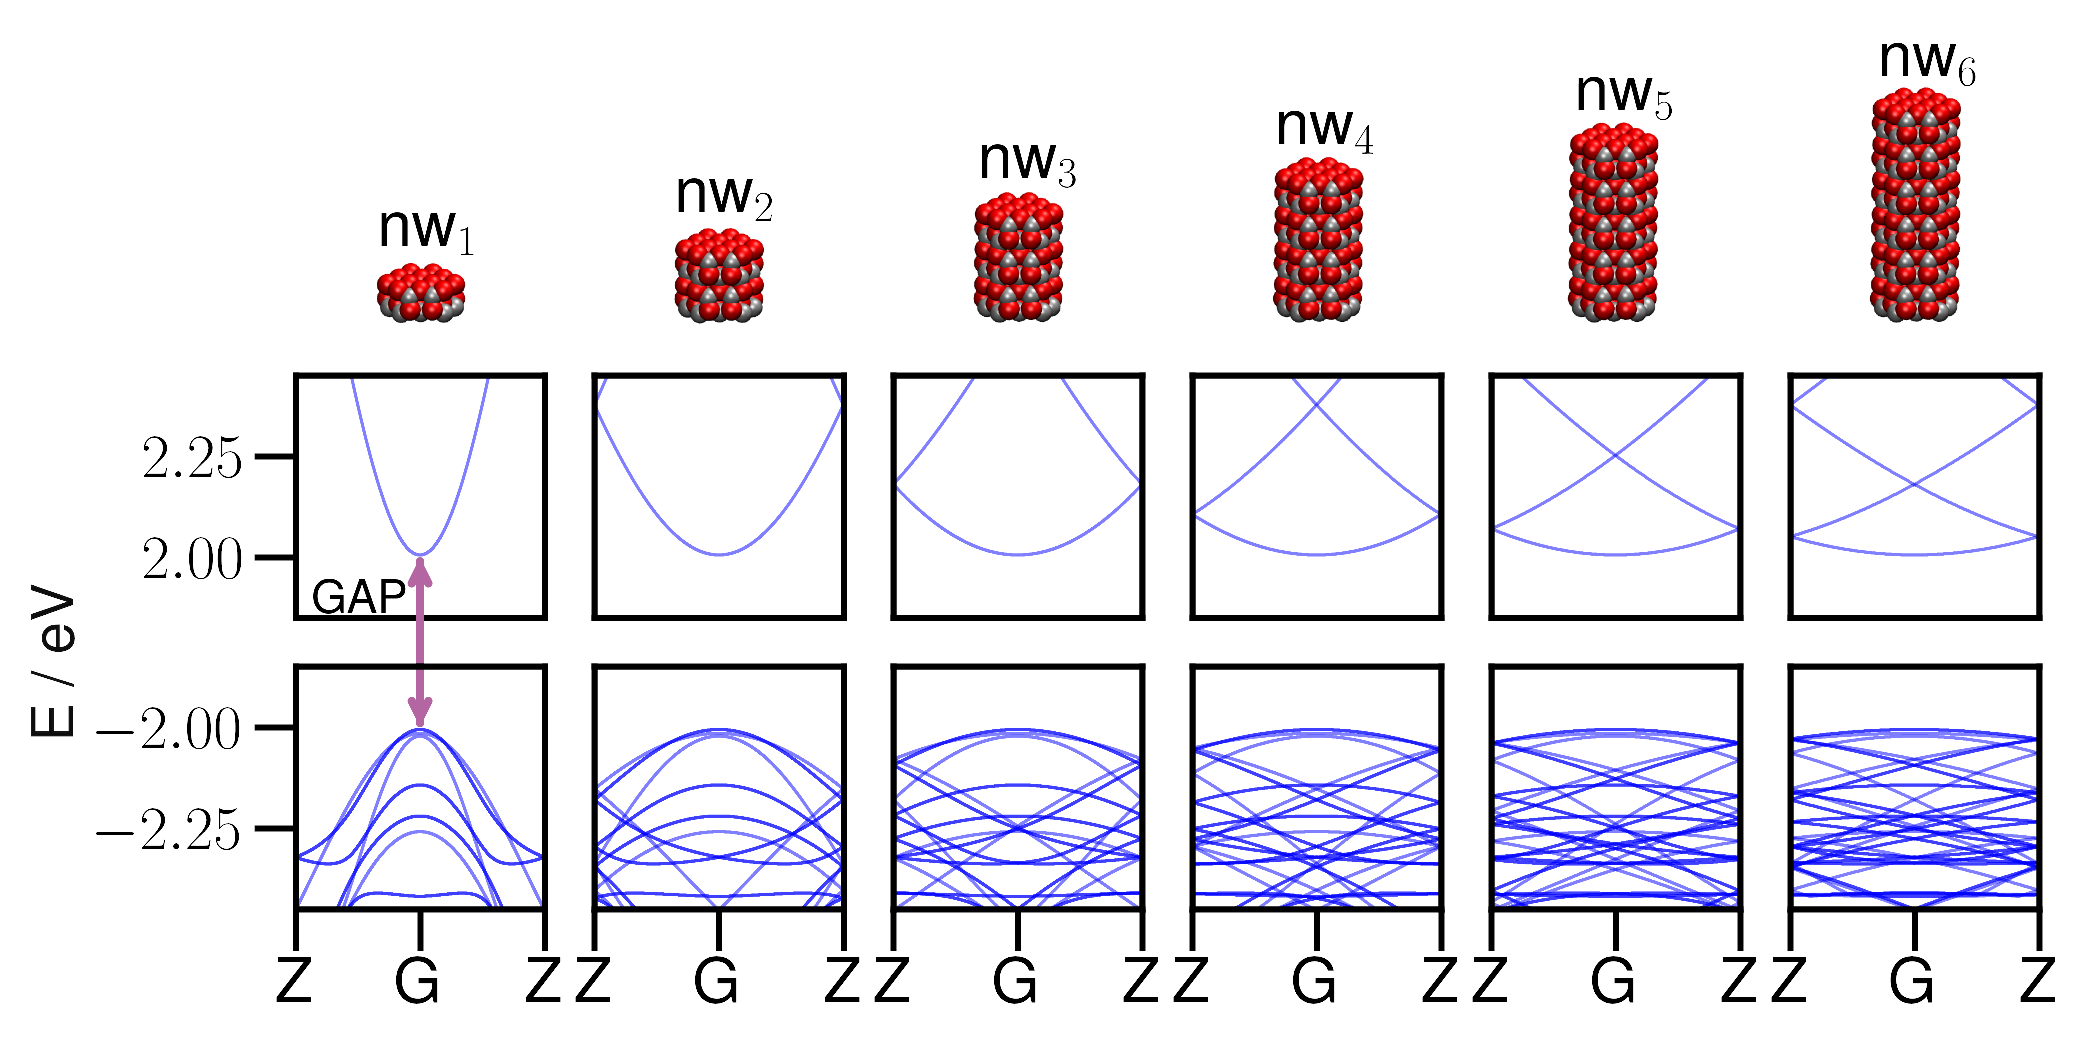
\includegraphics[height=7cm]{cap5/fig/bandas_nw_F.eps}
\caption{Estructura de bandas simuladas con dftb+ de los nws aislados. Se grafica la energía en función del vector de onda {\bf k}}
\label{bandas_nw_aislados}
\end{figure}


En los gráficos de bandas se pueden observar las bandas de valencia y conducción, la BV con valores negativos de energía desde $-2$ eV y la BC con energías positivas a partir de $2$ eV. El GAP es de aproximadamente $4.00$ eV como muestra la flecha, calculado como la diferencia de energía entre el borde de la BC y el borde de la BV que se encuentra en G (mínima energía). Este valor se mantiene constante a medida que aumenta la altura en las superceldas, la cual tiene sentido ya que estamos tratando con el mismo material independientemente de la cantidad de átomos utilizados. 

Si bien el GAP se mantiene constante, se pueden observar cambios en las bandas como por ejemplo el plegamiento de las mismas a medida que aumenta la altura o el número de átomos en la supercelda. Este efecto es típico en sistemas periódicos y se puede explicar utilizando un sistema simple como por ejemplo una cadena de moléculas 1D o un polímero, con 1 o 2 átomos por celda unidad tal como lo describe Yang \emph{et al.} en su trabajo publicado en 2018 \cite{Yang2018} (ver figura \ref{plegado}).

\begin{figure}[!htb]
\centering
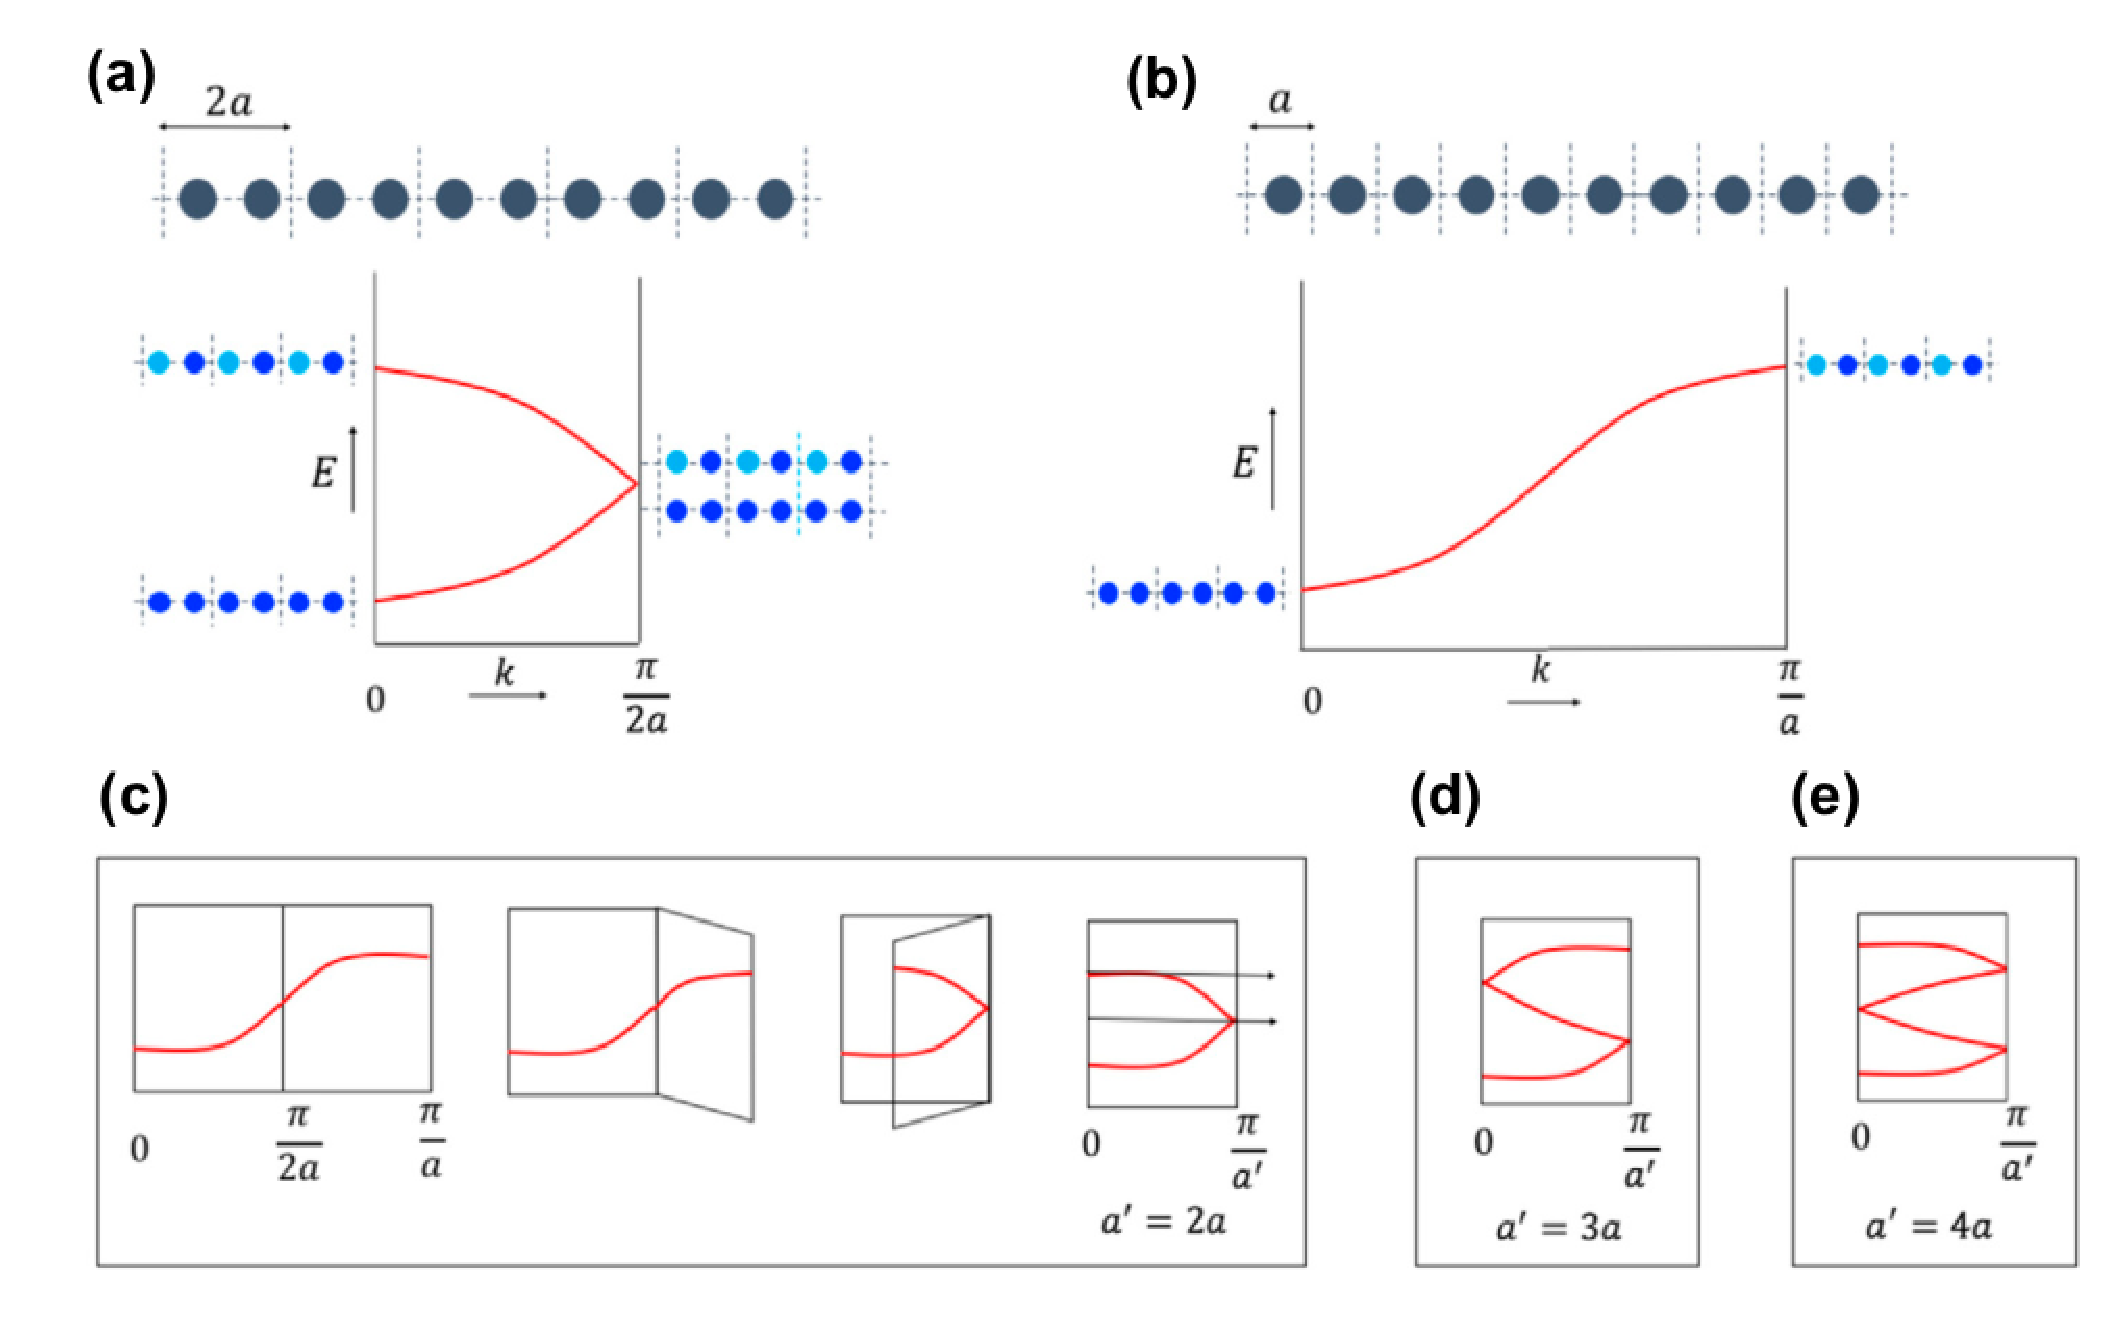
\includegraphics[height=7cm]{cap5/fig/plegado.eps}
\caption{Plegado de bandas en polímeros unidimensionales. {\bf(a)} Estructura de bandas de un polímero en el que hay dos átomos por celda unidad. Las bandas contienen dos ramas que se cruzan en ${\bf k}= \pi/2a$. {\bf(b)} Estructura de banda de un polímero en el que hay un átomo por celda unidad. La zona de brillouin se duplica porque la celda unidad es la mitad que en {\bf(a)}. {\bf(c)} Producción de la estructura de la banda en {\bf(a)} mediante el plegado de la estructura de la banda en {\bf(b)}. {\bf(d)} - {\bf(e)} La ampliación de la celda unidad provoca la multiplicidad de bandas. Las bandas se doblan tres veces cuando la celda unidad se triplica, cuatro veces cuando se cuadriplica. Extraído de \cite{Yang2018}}
\label{plegado}
\end{figure}


Si consideramos en primer lugar el sistema con 2 átomos por celda unidad como se expone en la figura \ref{plegado}{\bf(a)}, observamos que las bandas contienen 2 ramas, una hacia arriba desde los orbitales enlazantes y una hacia abajo desde los orbitales antienlazantes. Las mismas se cruzan en ${\bf k}= \pi/2a$ donde $2a$ es la longitud de la celda. Cuando la celda tiene 1 sólo átomo como se muestra en {\bf(b)}, la ZB se duplica ${\bf k}= \pi/a$ debido a que la longitud de la celda unidad es la mitad con respecto al caso anterior. Dado que la estructura de bandas no debería depender de la elección de la celda unidad, la estructura de bandas de {\bf(a)} y {\bf(b)} tienen que brindar la misma información. Esto podría entenderse como que la figura {\bf(a)} es la figura {\bf(b)} “plegada”, tal como se muestra en {\bf(c)}. Por último, las figuras {\bf(d)} y {\bf(e)} muestran que el proceso de plegado de bandas se puede continuar, es decir que si la celda unidad se triplica, la banda se doblará como se observa en {\bf(d)} y así sucesivamente. 


\begin{figure}[!htb]
\centering
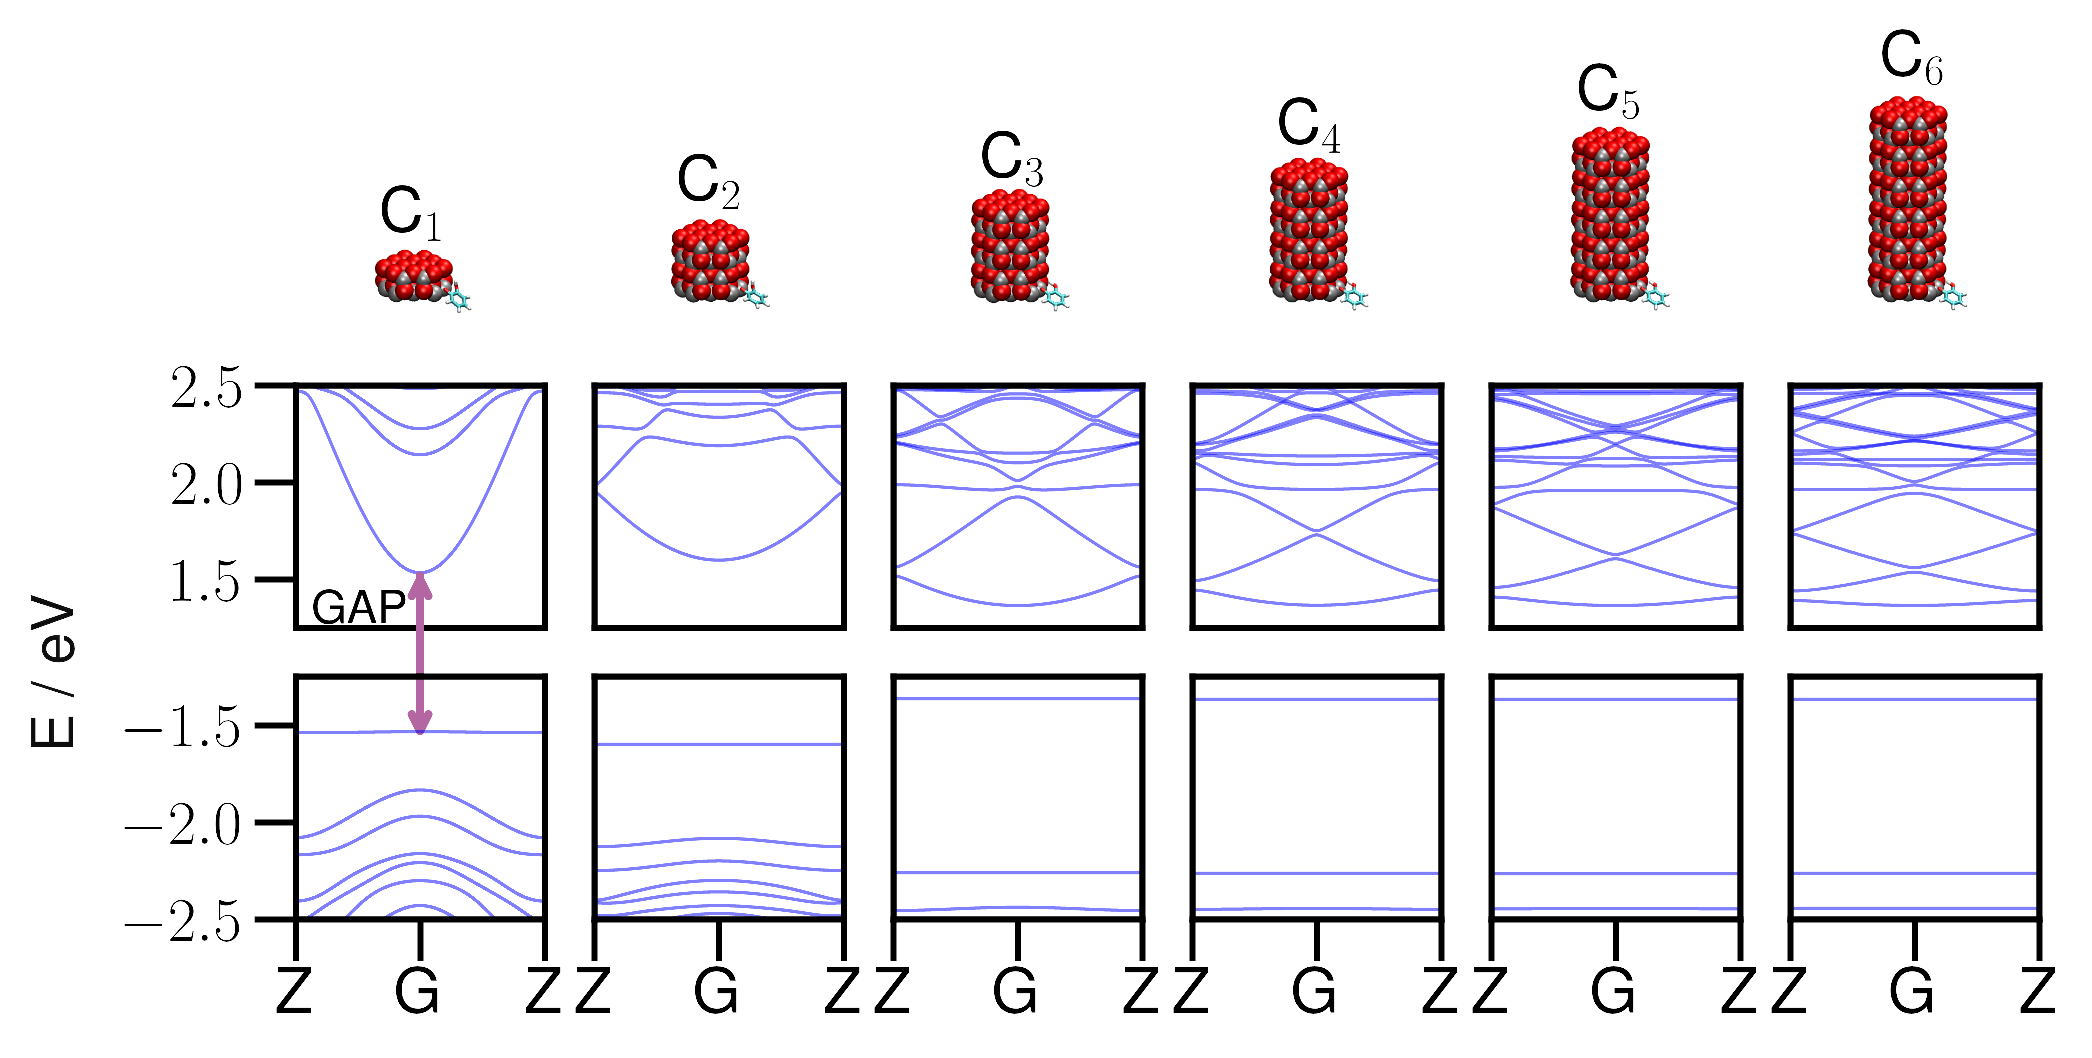
\includegraphics[height=7cm]{cap5/fig/bandas_C_F.eps}
\caption{Estructura de bandas simuladas con dftb+ de los nws aislados. Se grafica la energía en función del vector de onda {\bf k}}
\label{bandas_complex}
\end{figure}


A continuación en la figura \ref{bandas_complex} se muestran los gráficos de los cálculos de estructura de bandas para los complejos CAT-nw, es decir después de que el catecol se adsorba a la superficie del nw. A simple vista se observan varias diferencias con respecto a las bandas del nw aislado (ver figura \ref{comp_bandas}), sin embargo, es importante destacar que tanto el plegado de bandas se sigue observando en las bandas porque sigue siendo un sistema periódico. La disminución a aproximadamente $3$ eV del GAP es uno de los cambios más notables, este valor oscila en los sistemas más pequeños hasta estabilizarse con las superceldas de más átomos, es decir los complejos C$_3$, C$_4$ C$_5$ y C$_6$. 

\begin{figure}[!htb]
\centering
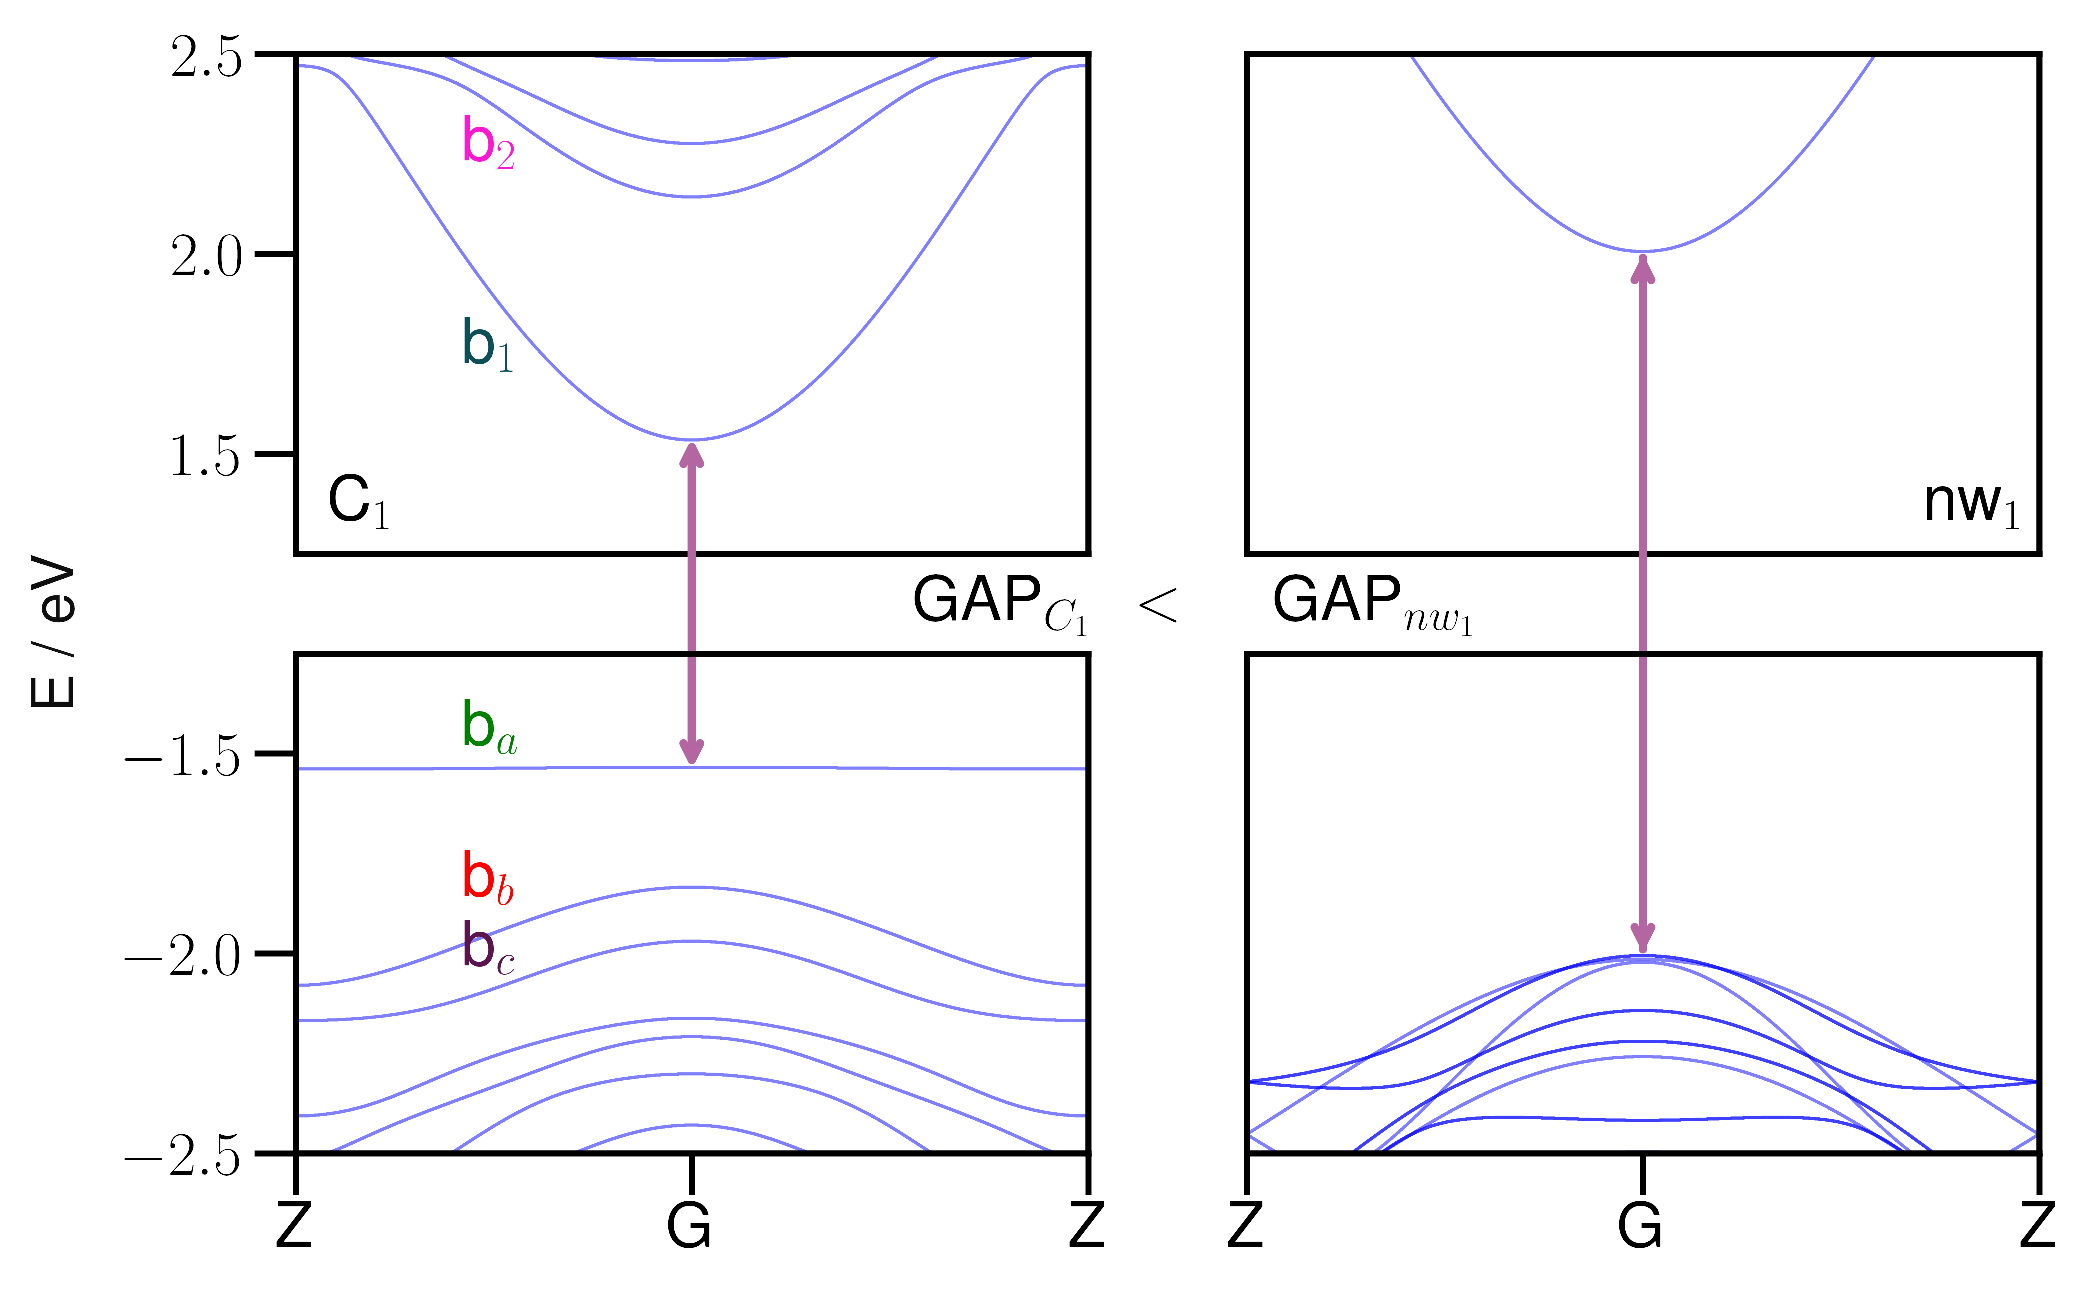
\includegraphics[height=7cm]{cap5/fig/comp_bandas.eps}
\caption{Comparación de los gráficos de estructura de bandas de C$_1$ {\bf (izquierda)} y nw$_1$ {\bf (derecha)}}
\label{comp_bandas}
\end{figure}

\newpage

También hay importantes diferencias en la BV y por esta razón nos enfocaremos (en este capítulo) en el análisis de las 3 bandas de mayor energía para cada sistema como muestra la figura \ref{comp_bandas}. Asignamos a la banda más energética de la BV como b$_a$ y las que siguen en energía como b$_b$ y b$_c$. Para estudiar cuáles son las contribuciones en cada una de las bandas recurrimos a las gráficas de orbitales moleculares (OM) (en el punto G) como se muestra a continuación en la figura \ref{om}. Realizando un análisis en simultáneo de la estructura de bandas y los OM podremos obtener una visión más clara de los cambios en la estructura electrónica al formarse el complejo.  

\begin{figure}[!htb]
\centering
\includegraphics[height=13.5cm]{cap5/fig/om.eps}
\caption{Esquema de los orbitales moleculares para cada uno de los sistemas estudiados correspondientes al punto G de la bandas b$_a$ (verde), b$_b$ (rojo) y b$_c$ (violeta) de la BV.}
\label{om}
\end{figure}


En este contexto, es importante destacar la aparición de una nueva banda, b$_a$, en la BV del gráfico de estructura de bandas de los complejos como consecuencia de la absorción del CAT, la cual cuenta con una energía alrededor de $-1.5$ eV y es una de las mayores responsables de la disminución del GAP. El orbital molecular correspondiente a esta banda se encuentra localizado en el colorante en todos los sistemas (ver figura \ref{om}), de manera que la misma está asociada al catecol. Las bandas que no dependen del vector de onda {\bf k} como ocurre en este caso, son llamadas bandas sin dispersión. 

Conforme a la figura \ref{bandas_complex}, b$_b$ y b$_c$ son bandas sin dispersión solo para los complejos C$_3$, C$_4$, C$_5$ y C$_6$. A priori podríamos decir que también están relacionadas con transiciones del catecol en acuerdo con los resultados obtenidos para b$_a$. En los sistemas C$_1$ y C$_2$, en cambio, las bandas b$_b$ y b$_c$ tienen dispersión ya que en estos casos la energía depende de {\bf k}. Si estudiamos los gráficos de la figura \ref{om} correspondientes a estas bandas (rojo para b$_b$ y violeta para b$_c$) encontramos 2 tipos de OM. El primer tipo corresponde a los complejos C$_3$, C$_4$, C$_5$ y C$_6$ donde los OM de la banda b$_b$ se encuentran localizados en el catecol y los OM de la banda b$_c$ están localizados en el sitio de unión CAT-nw, tal como lo habíamos predecido. Es decir que efectivamente las bandas sin dispersión involucran OM localizados con contribuciones predominantes del colorante. El segundo tipo de OM se observa en los casos C$_1$ y C$_2$ donde la dispersión de las bandas se fundamenta en la distancia entre catecoles de celdas vecinas. Cuando las moléculas de CAT se encuentran a una distancia lo suficientemente cortas, los OM que estaban localizados en el catecol interaccionan con los OM de los catecoles de celdas contiguas hasta formar un OM deslocalizado a lo largo del nw pero ubicado cercano al sitio de unión CAT-nw. La deslocalización de los OM otorga una estabilidad extra en C$_1$ y C$_2$ con respecto a los demás complejos lo cual se ve reflejada en la dispersión de las bandas b$_b$ y b$_c$. Esta es la razón por la que E$_{ad}$ es más negativa en estos sistemas. 


\section{Estructura electrónica de no equilibrio}

\subsection{Espectros de absorción}

Para obtener información sobre las excitaciones electrónicas se calcularon los espectros de absorción óptica del CAT y nw aislados y de los complejos (ver figura \ref{specs}) aplicando una perturbación tipo pulso para excitar todas las frecuencias del sistema. Los espectros de los sistemas aislados muestran bandas de absorción a partir de $4.0$ eV ya que a energías menores es ópticamente transparente. De la figura \ref{specs_cat} sabemos que el catecol absorbe a partir de $4.5$ eV aproximadamente y por eso no se observa en el espectro ya que en el mismo se contempla el rango solar. En el mismo también se aprecian bandas a partir de $4$ eV, las cuales se deben a las absorciones de las distintas superceldas de nw de acuerdo al GAP observado en los gráficos de estructura de bandas (figura \ref{bandas_nw_aislados}). Estos valores de energía corresponden a radiación UV en el espectro electromagnético.

Los espectros de absorción de los complejos CAT-nw presentan diferencias con respecto a los espectros de los componentes aislados, el cambio más evidente y el que más nos interesa es la aparición de nuevas bandas de absorción en el rango ($2.7-4$) eV.

\begin{figure}[!htb]
\centering
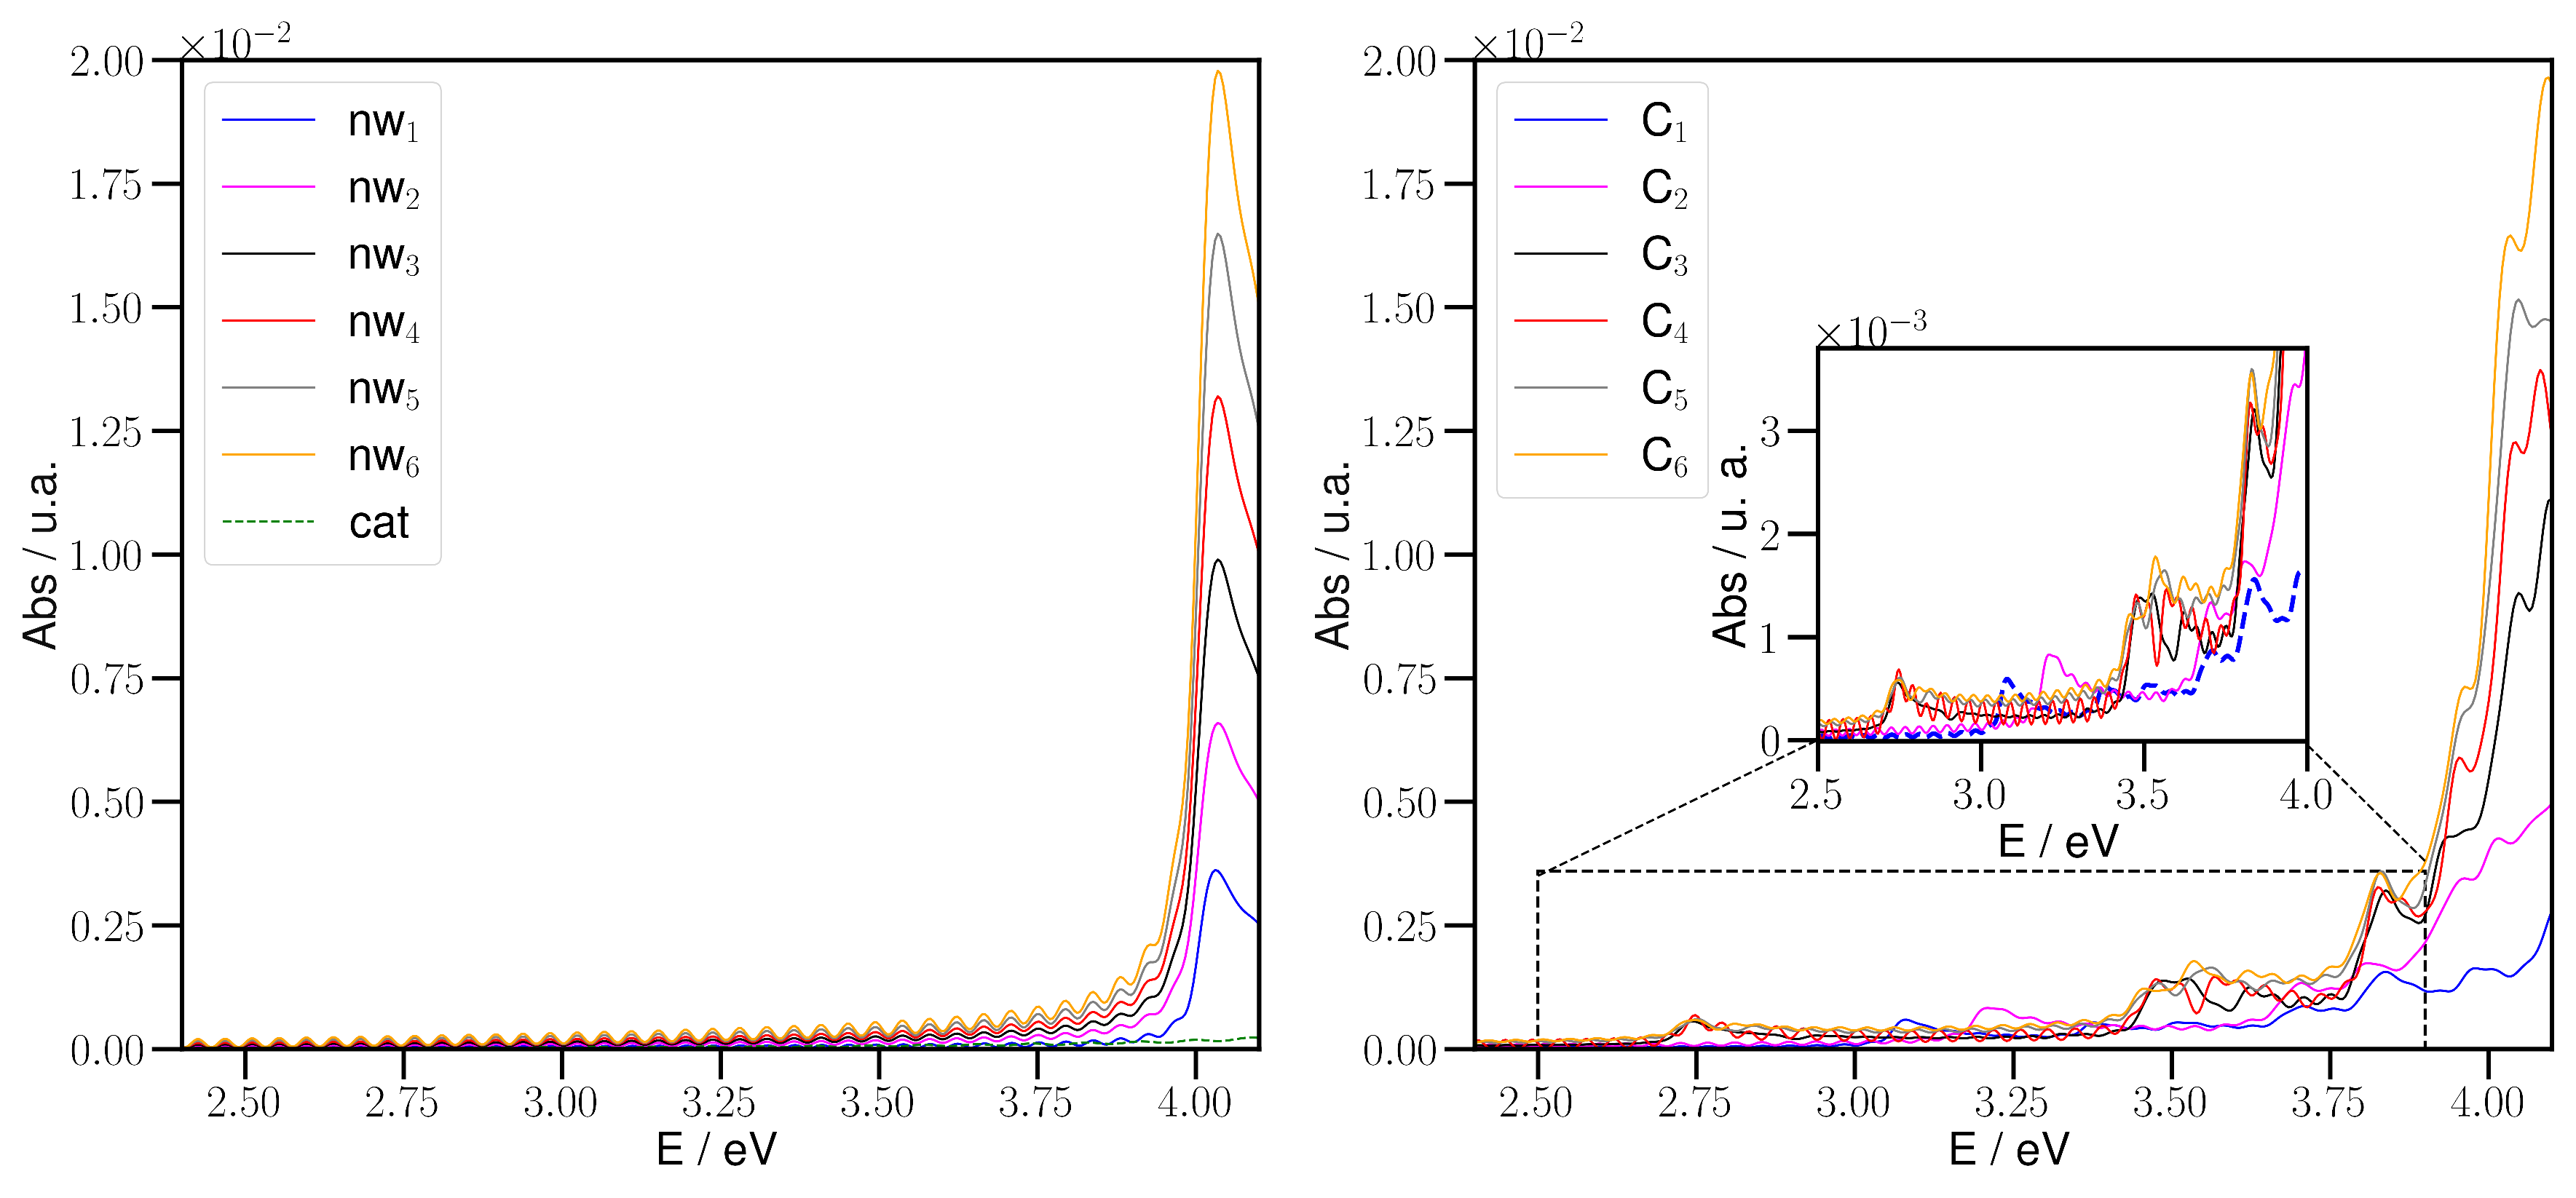
\includegraphics[height=6.5cm]{cap5/fig/specs.eps}
\caption{Espectros de absorción simulados con dftb+ ({\bf izquierda}) nw$_x$ y CAT aislado ({\bf derecha}) complejos C$_x$}
\label{specs}
\end{figure}

Si nos enfocamos solo en las bandas de menor energía para cada complejo, observamos que C$_3$, C$_4$, C$_5$ y C$_6$ tienen el máximo de absorción en $2.7$ eV, $C_1$ en $3.08$ eV y C$_2$ en $3.2$ eV. Estos resultados nos muestran que tanto el catecol como los nw son transparentes a la luz visible cuando se encuentran separados. Sin embargo, la absorción de la molécula a la superficie del SC genera transiciones en el rango visible como es el caso de los sistemas C$_1$, C$_3$, C$_4$, C$_5$ y C$_6$ o en el límite UV-visible para C$_2$. 
     
Existe un intereés particular en C$_1$ (línea punteada de la figura \ref{specs}), debido a que presenta la E$_{ad}$ más negativa y por ende es el sistema con la unión CAT-nw más fuerte. Por esta razón, a continuación se plantea un análisis más profundo de este complejo. En primer lugar se presentan todos los gráficos de estructura electrónica en el equilibrio como son los cálculos de densidades de estado y estructura de bandas para este sistema junto con los espectros de absorción tal como muestra la figura \ref{dos_bandas_spec}. El conjunto de resultado ayudará a la comprensión de las transiciones que ocurren. 

\begin{figure}[!htb]
\centering
\includegraphics[height=5.7cm]{cap5/fig/dos_bandas_spec.eps}
\caption{(1) DOS C$_1$, pdos de CAT y nw$_1$, (2) Estructura de bandas para C$_1$, (3) Espectros de absorción de: C$_1$, nw$_1$ y CAT, (4) DOS nw$_1$ aislado y (5) Estructura de bandas del nw$_1$ aislado}
\label{dos_bandas_spec}
\end{figure}

En la figura \ref{dos_bandas_spec} (1) y (4) se muestran los cálculos de densidades de estados, en el primero la densidad de estados total (DOS) para C$_1$ y la densidad de estados proyectada ({\bf pdos}) del catecol y el nw$_1$ mientras que en el segundo la DOS del nw$_1$. La estructura de bandas para C$_1$ y nw$_1$, se observan en (2) y (5), respectivamente, y en el medio, los espectros de absorción de CAT y nw$_1$ aislados y C$_1$.      
  
La densidad de estados por unidad de volumen (o simplemente densidad de estados) en un cristal perfecto donde el potencial tiene la periodicidad de la red de Bravais subyacente tiene la forma:

\begin{equation}
\displaystyle g(E) =  \sum_{n} g_n(E), 
\label{eq:dos}
\end{equation}

donde la densidad de estados DOS(E) de la n-ésima banda se define como una integral de superficie \cite{Ashcroft76}:

\begin{equation}
\displaystyle DOS(E) =  \int_{S_n(E)} \frac{dS}{4\pi^3} \frac{1}{|\nabla E_n({\bf k})|}, 
\label{eq:dos_n}
\end{equation}

sea E$_n({\bf k})$ la energía de la n-ésima banda para los valores {\bf k} permitidos, S$_n$(E) la porción de la superficie E$_n({\bf k})$=E que se encuentra dentro de la celda primitiva y $\nabla E({\bf k})$ un vector normal a esa superficie cuya magnitud es igual a la tasa de cambio de E$_n({\bf k})$ en la dirección normal. Podemos relacionar los gráficos de densidad de estados y estructura de bandas utilizando la ecuación \ref{eq:dos_n}: E$_n({\bf k})$ es periódica en la red recíproca y en general diferenciable en todas partes y seguramente habrá valores de ${\bf k}$ en cada celda primitiva en los que $\nabla$E = 0. En los máximos y mínimos locales el gradiente es cero y en consecuencia el integrando de la densidad de estados diverge. 


Observamos que la DOS y ambas pDOS de C$_1$ de la figura \ref{dos_bandas_spec}(1) divergen para los valores de energías calculados en el punto G de la estructura de bandas (2) donde la derivada es cero. El gráfico (1) muestra cuáles son las especies que contribuyen con estados a las bandas, el catecol aporta estados a toda la b$_a$ (en $-1.5$ eV) sin dispersión mientras que el nw$_1$ aporta estados al resto de las bandas que tienen dispersión. Estos resultados coinciden con lo que hemos observado al graficar los OM (figura \ref{om}). En el gráfico (4) se observa la DOS del nw aislado con discontinuidades en los máximos y mínimos locales de la estructura de bandas (5).


El espectro de absorción de C$_1$ (3) señala con flechas las nuevas bandas que aparecen al formarse el complejo en el rango ($3-4$) eV. Se puede asignar en la estructura de bandas (2), mediante flechas de colores, cuáles son las transiciones que generan las absorciones en el espectro restando las energías en G entre 2 bandas y comparando esos valores con las energías de los máximos de absorción del espectro. Estas asignaciones se realizaron en G debido a que en este punto ocurren las transiciones de menor energía para cada banda. Por ejemplo, la banda en el espectro con máximo de absorción a $3.08$ eV (flecha negra) se corresponde con la diferencia energética entre el borde de la b$_c$ y la b$_a$, entonces suponemos que la absorción ocurre por la transición mencionada. Sin embargo, es necesario estudiar la naturaleza de las excitaciones de una manera más profunda analizando la evolución temporal de las poblaciones y de las cargas. Estos cálculos se llevaron a cabo perturbando el sistema con un campo eléctrico que oscila en el tiempo. Para ello se realizaron simulaciones de un láseres continuos sintonizados con las energías de interés, en este caso las energías que analizamos son $3.08$ eV, $3.38$ eV, $3.50$ eV, $3.70$ eV, $3.83$ eV y $3.97$ eV. 

\subsection{Evolución temporal de las cargas de Mulliken y de las poblaciones electrónicas}

\begin{figure}[!htb]
\centering
\includegraphics[height=7.2cm]{cap5/fig/cargas_3.08.eps}

\vspace{0.5cm}

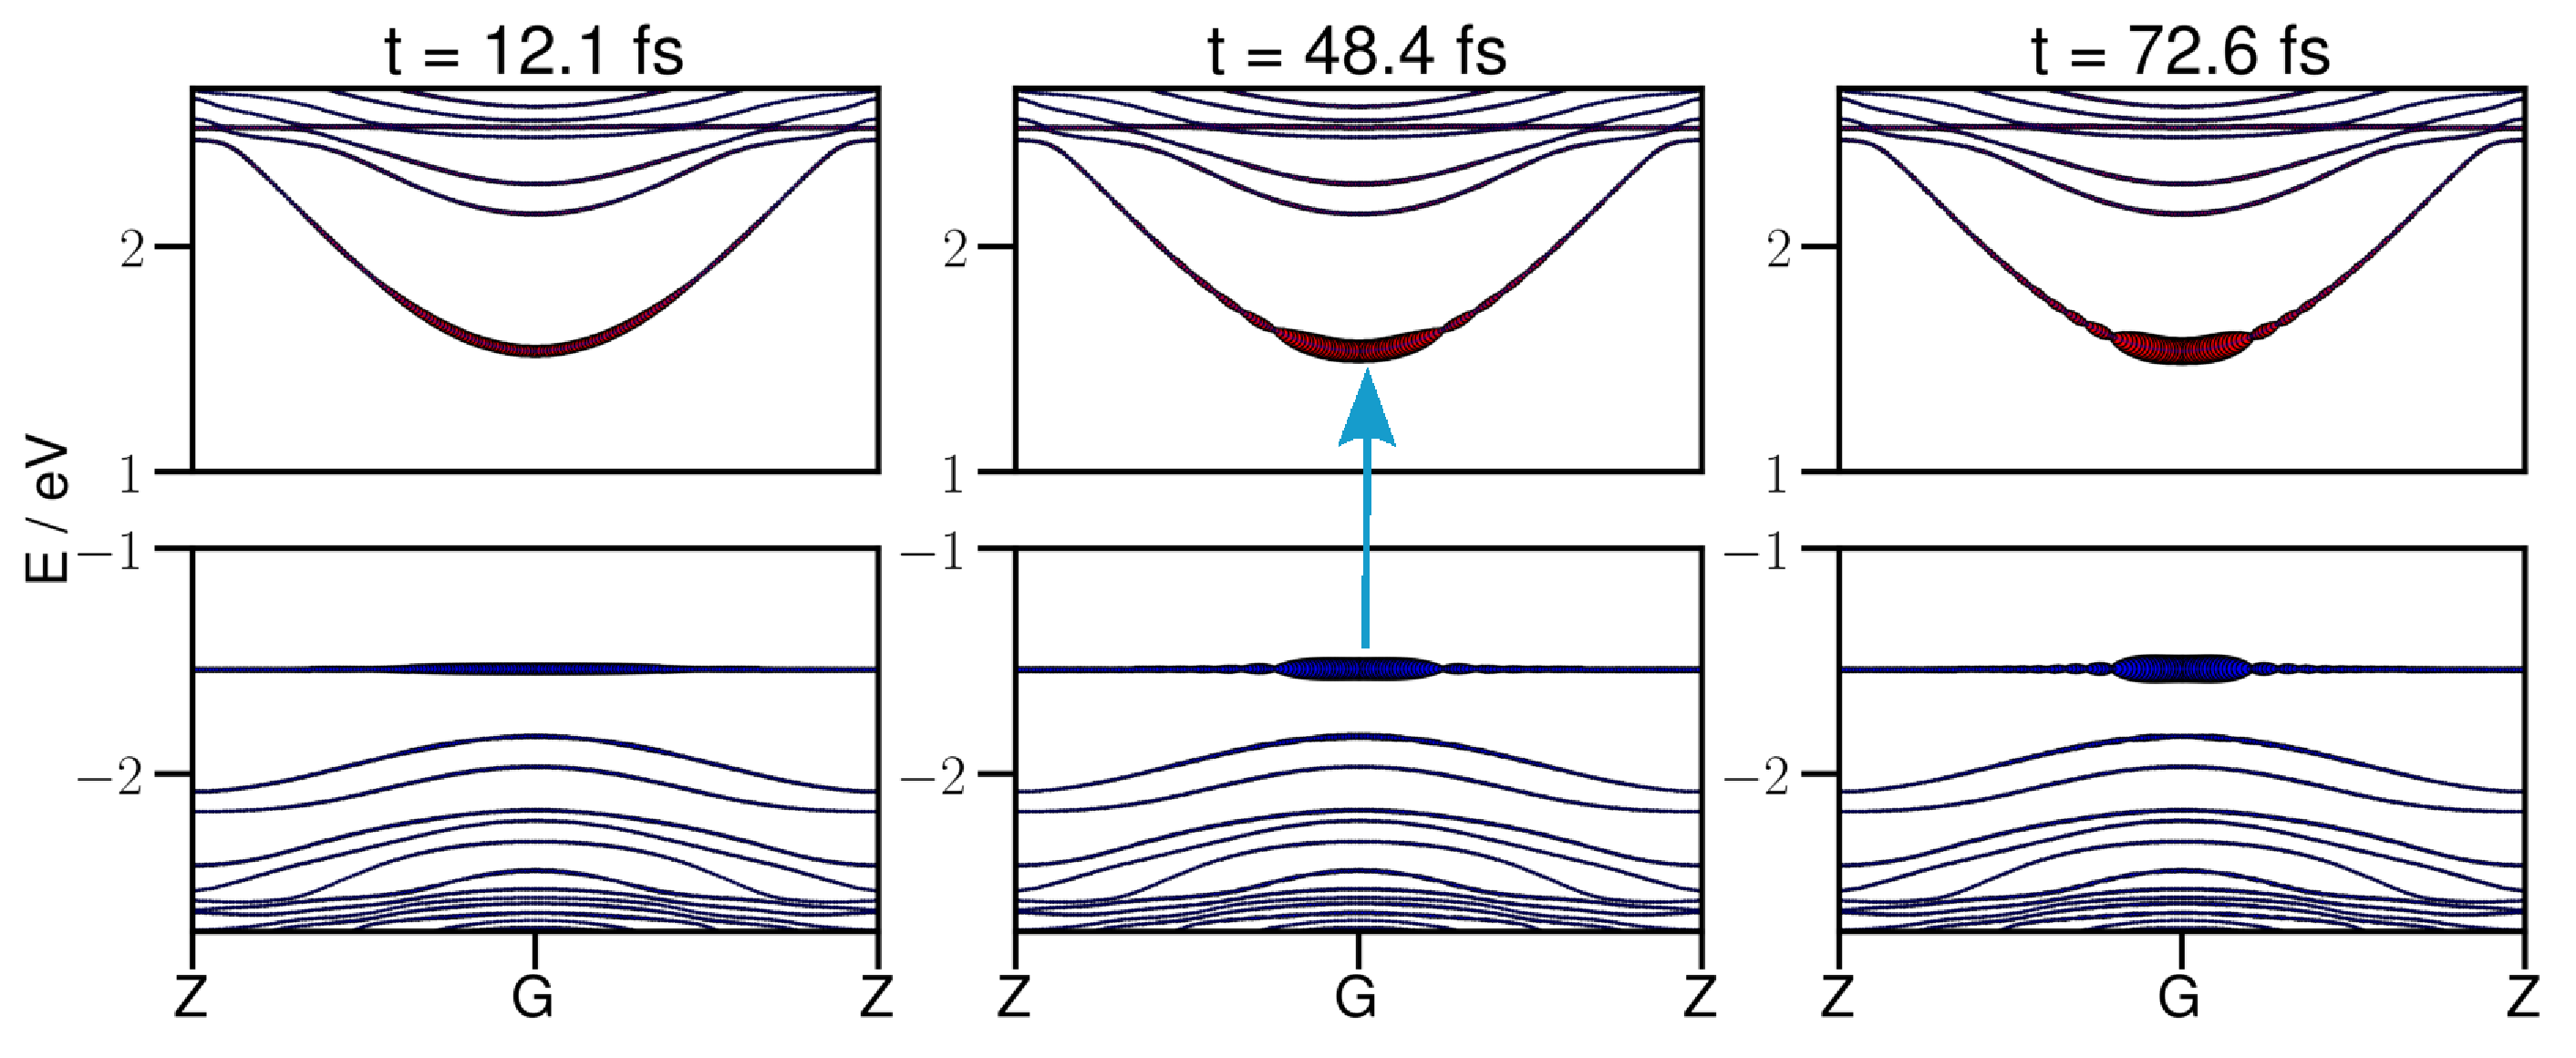
\includegraphics[height=6cm]{cap5/fig/dynpop_3.08_cut.eps}
\caption{ ({\bf Arriba}) izquierda: Espectro de absorción para C$_1$, CAT aislado y nw$_1$ aislado y derecha: cargas en función del tiempo al perturbar el sistema con un láser de $3.08$ eV. ({\bf Abajo}) estructura de bandas de C$_1$. Sobre las bandas se grafica la diferencia de población electrónica que se genera al iluminar C$_1$ con el láser a 3 tiempos distintos: en azul se representa la disminución de la población electrónica al iluminar y en rojo el aumento de la población electrónica al iluminar con el láser.}
\label{ilu_3.08}
\end{figure}


En primer se iluminó el sistema con un láser seteado a $3.08 eV$, es decir con el máximo de absorción de la banda menos energética (como señala la figura \ref{ilu_3.08}) durante $100$ fs. Para obtener información acerca de la evolución temporal de las cargas mientras el complejo C$_1$ es irradiado, se calcularon y graficaron las cargas de Mulliken en el periodo de tiempo mencionado (figura \ref{ilu_3.08} arriba a la derecha). Se observa del gráfico que a medida que transcurre el tiempo el nw va adquiriendo carga negativa (rosa) en la misma medida en la que el catecol (verde) se carga positivamente. Estos resultados indican que los electrones se inyectan desde el catecol a la BC del nw, es decir que la carga se transfiere desde el colorante al SC. Otra observación importante en el gráfico es que la dependencia entre las cargas y el tiempo es prácticamente lineal, lo cual señala que a dinámicas más largas la transferencia seguirá aumentando.  

La figura \ref{ilu_3.08} abajo muestra 3 gráficos de estructura de bandas de C$_1$. Sobre cada uno de ellos se graficó la diferencia de población electrónica que se genera al iluminar con el láser:


\begin{multline}
\Delta P = \textrm{Población electrónica cuando se ilumina con el láser} -  \\
           \textrm{Población electrónica antes de iluminar con el láser}
\end{multline} 


cuando $\Delta P$ es positivo, la población electrónica aumenta con la irradiación mientras que cuando $\Delta P$ arroja un valor negativo, la población electrónica disminuye. En los gráficos se muestran los valores de $\Delta P$ tomados en 3 tiempos distintos de la dinámica y se representa en rojo la diferencia de población positiva ($\Delta P$+) y en azul la diferencia de población negativa ($\Delta P$-).


A tiempos cortos ($12.1$ fs) el láser no llega a aportar la energía necesaria para generar una diferencia de población y en consecuencia se produzca la transición, en ese momento todas las transiciones son posibles. A medida que transcurre el tiempo, por ejemplo a la mitad de la dinámica ($48.4$ fs) se observa la disminución de población en b$_a$ a $-1.5$ eV y aumento en la banda menos energética de la BC, es decir b$_1$ (ver figura \ref{comp_bandas}). En el punto G (en ambas bandas) es donde se produce la mayor $\Delta P$ y por eso es allí donde ocurre la transición (flecha de color celeste). Tan pronto nos alejamos del centro de la ZB, $\Delta P$ comienza a disminuir y se observa la presencia de nodos (donde la $\Delta P$ = 0) a medida que esto ocurre. A tiempos más largos ($72.6$ fs), la transición observada es la misma pero la población electrónica cambia, $\Delta P$ se va localizando cada vez más en G y los nodos se muestran para valores diferentes de ${\bf k}$ con respecto al caso anterior. 

Los resultados obtenidos en los gráficos se puede explicar mediante la Regla de Oro de Fermi o la Regla de Oro de la Teoría de Perturbaciones dependiente del tiempo, la cual aplica la teoría perturbaciones dependiente del tiempo a un sistema que sufre una transición desde un estado inicial $\ket i$ a un estado final $\ket f$ que es parte de un continuo de estados es decir, cuando la energía pertenece a una parte continua del espectro de H$_0$ (hamiltoniano del sistema sin perturbar), entonces debemos tener en cuenta todos los estados a los que el sistema puede saltar. 
Para una gran cantidad de problemas, es suficiente la teoría de la perturbación independiente del tiempo. Sin embargo, hay casos en los que queremos estudiar cómo los sistemas responden a las perturbaciones impuestas y luego se establecen en estados estacionarios después de un intervalo, es decir, estudiar las transiciones inducidas por una perturbación entre estados estacionarios del sistema no perturbado. En casos como estos, utilizamos la teoría de la perturbación dependiente del tiempo para calcular, entre otras cosas, las probabilidades de transición. La ecuación de Schr\"odinger dependiente del tiempo para el sistema es \cite{Koukaras}: 

\begin{equation}
\displaystyle H \ket {\Psi (t)} = [H_0 + W(t)]  \ket {\Psi (t)} =  i \hbar \frac{\partial \ket {\Psi (t)}}{\partial t} 
\label{eq:sch_dep_t}
\end{equation}


donde se asume que el hamiltoniano H del sistema puede ser escrito de la forma $H = H_0 + W(t)$ donde $W(t)$ es la perturbación aplicada al sistema y que el estado del sistema $\ket {\Psi}$  al tiempo t, se expresa como una combinación lineal de las funciones base ${\phi_n}$: 


\begin{equation}
\displaystyle \ket {\Psi (t)} = \sum_n c_n(t) \ket {\Psi_n (t)} = \sum_n c_n(t) \ket {\phi_n (t)} e^{\frac{-i E_n(t)}{\hbar}}   
\label{eq:base}
\end{equation}


Las funciones base $\phi_n$ provienen de la ecuación de Schr\"odinger independiente del tiempo del sistema sin perturbar ($H_0 \phi_n  = E_n \phi_n$) y están relacionadas con las funciones de onda no perturbadas dependientes del tiempo por

\begin{equation}
\displaystyle \ket {\Psi_n (t)} = \ket {\phi_n (t)} e^{\frac{-i E_n(t)}{\hbar}}   
\label{eq:relaciones_func_onda}
\end{equation}

Al insertar la relación \ref{eq:base} en \ref{eq:sch_dep_t} y proyectando el resultado en $\phi_n$ obtenemos:

\begin{equation}
\displaystyle    \frac{\partial c_n(t)}{\partial t}  = \frac{1}{i\hbar} \sum_k c_k(t) W_{nk} (t) e^{i w_{nk} t)}
\label{eq:coeff_s_aprox}
\end{equation}

donde $W_{nk} = \bra {\phi_n} W(t) \ket {\phi_k}$ son los elementos de matriz de la perturbación y $w_{nk}$ es $\frac{E_n-E_k}{\hbar}$

Para evaluar los coeficientes de \ref{eq:coeff_s_aprox} suponemos que: {\bf (a)} el sistema está inicialmente en el estado $\ket{i}$, por lo tanto, todos los coeficientes en t = 0 son iguales a cero, excepto para $c_i$: $c_j$ (t = 0) = $\delta_{ij}$ y {\bf (b)} la perturbación es muy débil y se aplica durante un corto período de tiempo, de modo que todos los coeficientes permanecen casi sin cambios. Entonces la ecuación \ref{eq:coeff_s_aprox} ahora se transforma en:


\begin{equation}
\displaystyle \frac{\partial c_n(t)}{\partial t} = \frac{1}{i\hbar} c_i(t) W_{ni} (t) e^{i w_{ni} t)}
\label{eq:coeff_c_aprox}
\end{equation}

así que para cualquier estado final el coeficiente será: 

\begin{equation}
\displaystyle \frac{\partial c_n(t)}{\partial t} = \frac{1}{i\hbar} \int_0^t W_{fi} (t') e^{i w_{fi} t')} dt'
\label{eq:coeff_final}
\end{equation}

La aplicación de la perturbación cambia el estado del sistema desde el estado inicial $\ket{\phi_i}$ a un estado final $\ket{\phi_f}$, ambos son estados propios del hamiltoniano no perturbado H$_0$. La probabilidad de encontrar el sistema en el estado propio $\ket{\phi_f}$ es: 


\begin{equation}
\displaystyle P_{if}(t) = {|\langle\phi_f |\psi(t) \rangle |}^2
\label{eq:prob_1}
\end{equation}

y utilizando \ref{eq:coeff_final} obtenemos:

\begin{equation}
\displaystyle P_{if}(t) = \frac{1}{\hbar^2} \left| \int_0^t W_{fi} (t') e^{i w_{fi} t')} dt'\right |^2
\label{eq:prob_2}
\end{equation}

Una perturbación oscilante (como un láser) está definida de la forma:

\begin{equation}
\displaystyle W(t) = 2 W \cos(wt) = 2 (e^{i w t} + e^{-i w t})
\label{eq:pert_laser}
\end{equation}

Insertando esta ecuación en \ref{eq:coeff_final} obtenemos:


\begin{align}
\displaystyle c_f(t) &= \frac{W_{fi}}{i\hbar} \left\lbrace\frac{e^{i(w_{fi} + w) t)}-1}{i (w_{fi} + w)} + \frac{e^{i (w_{fi} - w) t)}-1}{i (w_{fi} - w)}\right\rbrace
\label{eq:coeff_final_oscilante}
\end{align}


Entonces la ecuación \ref{eq:prob_2} se transforma en (e introduciendo la función $F(t,w-w_{fi}$):


\begin{align}
\displaystyle P_{if}(t) &= \frac{W_{fi}^2}{\hbar^2} \left|\frac{e^{i(w_{fi} + w) t)}-1}{i (w_{fi} + w)} + \frac{e^{i (w_{fi} - w) t)}-1}{i (w_{fi} - w)}\right|^2  \\
&= \frac{W_{fi}^2}{\hbar^2} F(t,w-w_{fi})
\label{eq:prob_final}
\end{align}

Cuando el estado final es parte de un continuo de estados la probabilidad se obtiene integrando la probabilidad dada por la ecuación \ref{eq:prob_final} con la densidad de estados $\rho(E)$ como peso: 


\begin{equation}
\displaystyle P(t) = \int_{Eacc} P_{if}(t) \rho(E) dE
\label{eq:prob_osc}
\end{equation}

donde ${Eacc}$ denota todos los estados a los que el sistema puede saltar bajo la influencia de la perturbación. Sustituyendo \ref{eq:prob_final} en \ref{eq:prob_osc} obtenemos:

\begin{equation}
\displaystyle P(t) = \int_{Eacc} \frac{W_{fi}^2}{\hbar^2} F(t,w-w_{fi}) \rho(E) dE
\end{equation}

como el rango de energías es muy estrecho, el elemento de matriz $W_{fi}$ y la densidad de estados $\rho(E)$ se pueden considerar como constantes. Entonces la probabilidad es una integral de $F(t, w-wfi)$:

\begin{equation}
\displaystyle P(t) = \frac{W_{fi}^2}{\hbar^2} \rho(E) \int_{Eacc} F(t,w-w_{fi})dE
\label{eq:prob_osc_final}
\end{equation}


En la figura \ref{fermi_F} se observa un gráfico de $F(t,w)$ en función de w, a 4 tiempos distintos, donde $t1<t2<t3<t4$

\begin{figure}[!htb]
\centering
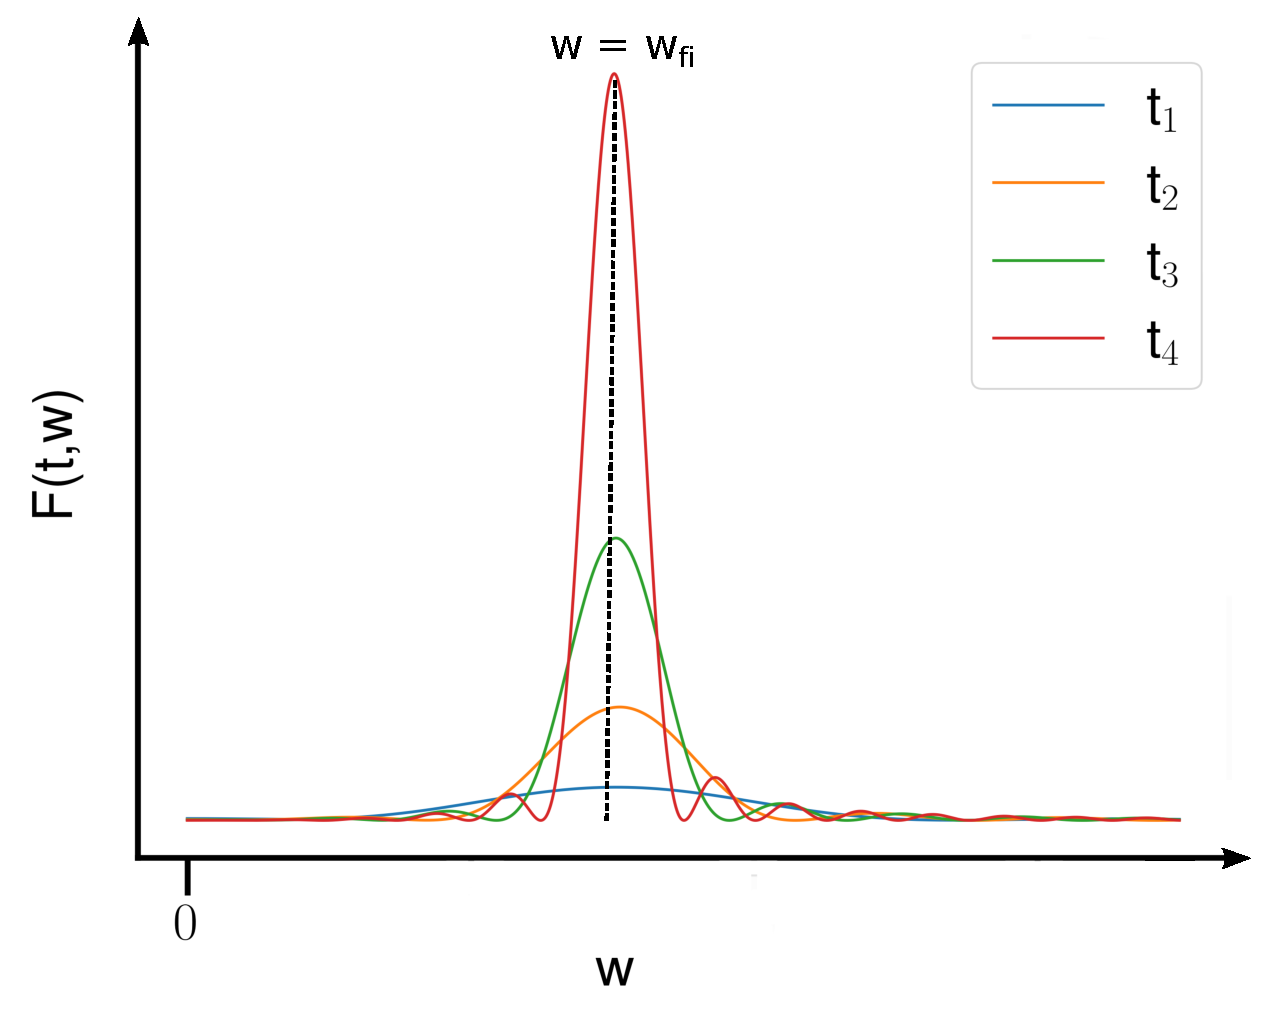
\includegraphics[height=7.8cm]{cap5/fig/fig_nodos_cut.eps}
\caption{$F(t,w)$ vs w, donde $F(t,w)$ actúa como una función delta de Dirac para 4 tiempos donde $t1<t2<t3<t4$´}
\label{fermi_F}
\end{figure}


Los cuatro gráficos representan a $F(t,w)$ como una función con un pico centrado en $w = w_{fi}= \frac{E_f-E_i}{\hbar}$ y valores de w donde $F(t,w) = 0$ o la probabilidad es cero (nodos). A medida que el sistema evoluciona temporalmente, la función se va haciendo más aguda en w$_{fi}$, es decir que en t=$\inf$ F es una función delta de Dirac. Simultáneamente, los nodos toman valores que se van acercando cada vez más a w$_{fi}$.


$F(t,w)$ justifica entonces la concentración de $\Delta P$ en la frecuencia de resonancia (que se muestra en G) con el aumento del tiempo, tal como se observó en la figura \ref{ilu_3.08}. Luego, al graficar las diferencias de poblaciones electrónicas a los 4 tiempos mencionados anteriormente utilizando la Regla de Oro de Fermi encontramos que el modelo planteado representa cualitativamente los cálculos obtenidos con dftb+ (ver figura \ref{fermi_bandas}). 


\begin{figure}[!htb]
\centering
\subfloat[t$_1$]{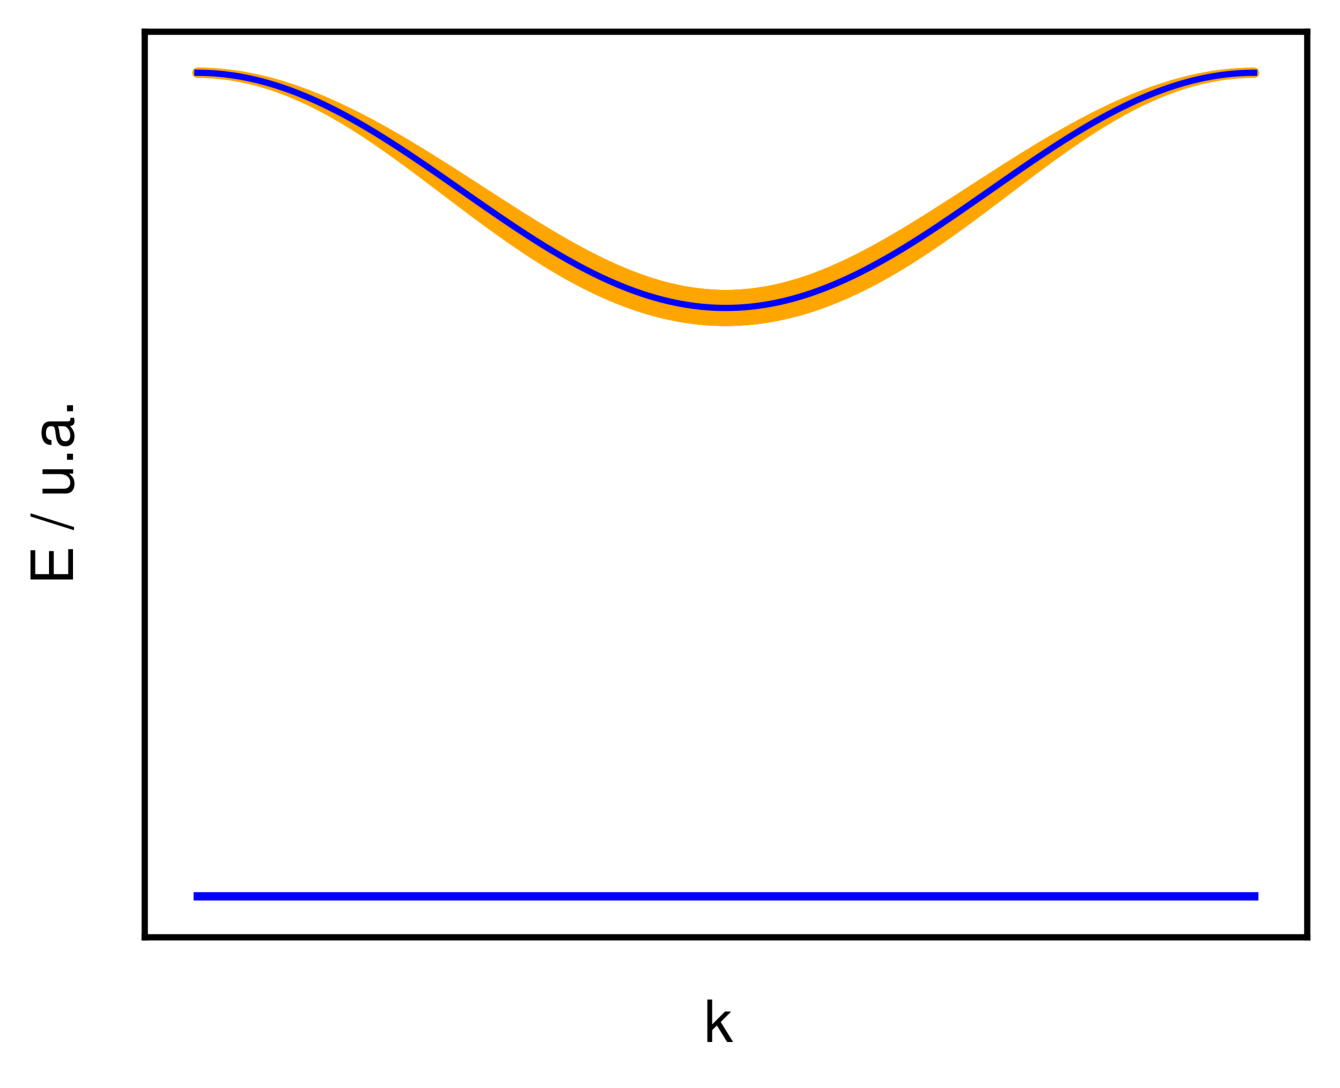
\includegraphics[height=6cm]{cap5/fig/fig_time1.eps}}
\subfloat[t$_2$]{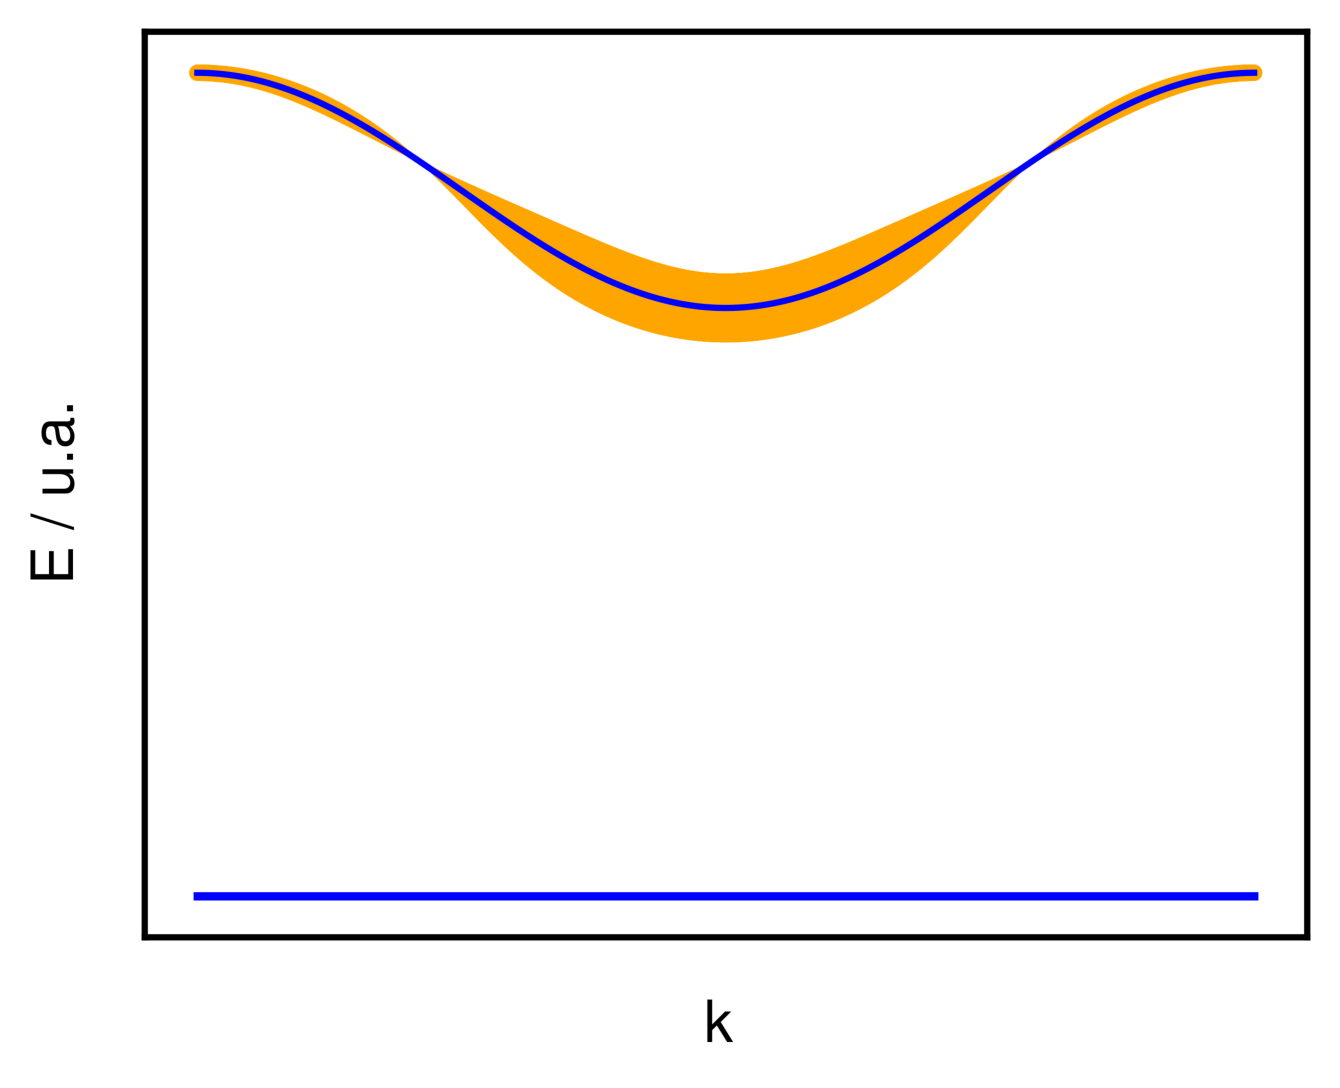
\includegraphics[height=6cm]{cap5/fig/fig_time2.eps}}


\subfloat[t$_3$]{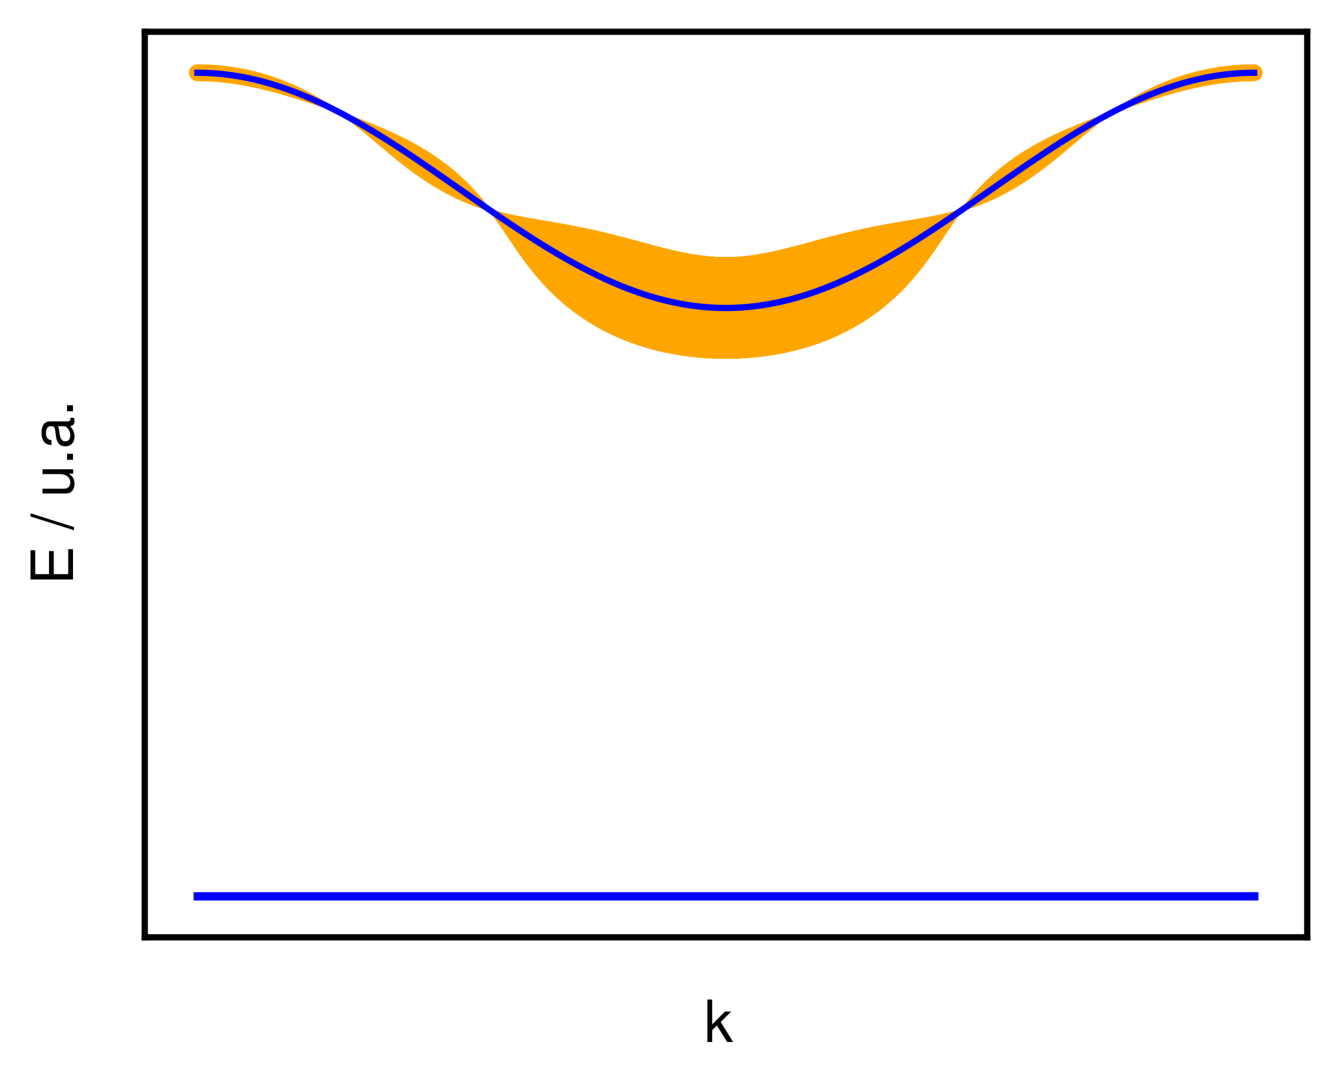
\includegraphics[height=6cm]{cap5/fig/fig_time3.eps}}
\subfloat[t$_4$]{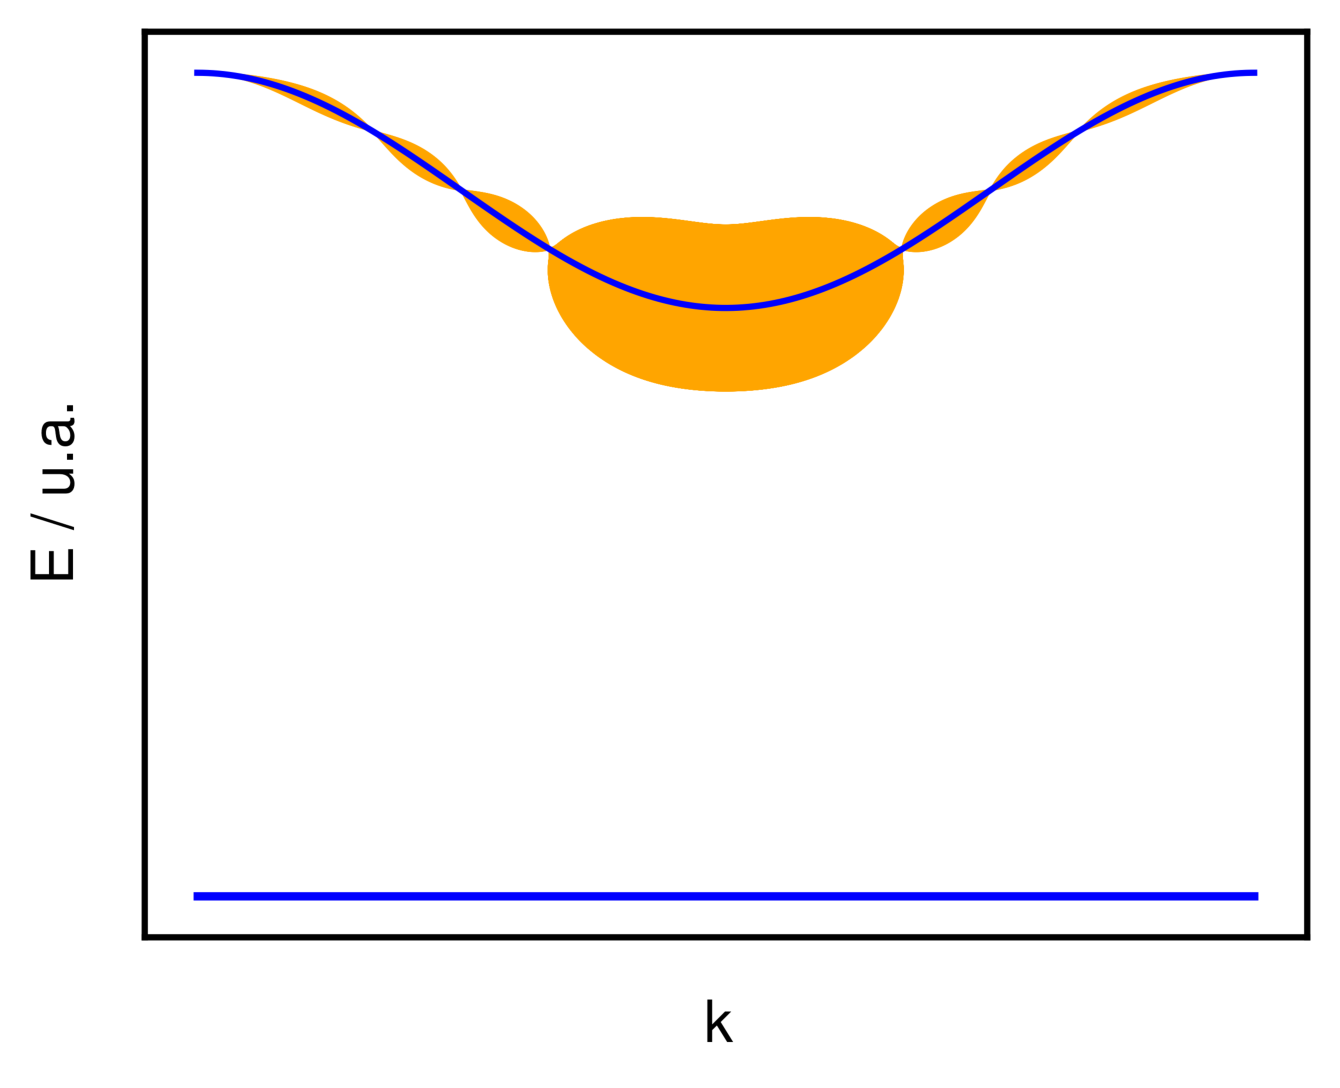
\includegraphics[height=6cm]{cap5/fig/fig_time4.eps}}
\caption{Estructura de bandas (azul) y $\Delta P$ (naranja) cuando el estado final es parte de un continuo de estados de acuerdo a la Regla de Oro de Fermi para 4 tiempos, donde $t1<t2<t3<t4$}
\label{fermi_bandas}
\end{figure}

Estos resultados, los cuáles obedecen la regla de oro de Fermi, no sólo permite explicar la evolución de las poblaciones electrónicas simuladas cuando iluminamos C$_1$ con un láser sintonizado a $3.08$ eV sino que también permite explicar la relación entre las transiciones que ocurren y la transferencia de carga. En ese caso, la transición más probable se produce en G y es la responsable de la banda a $3.08$ eV del espectro de absorción y de la transferencia de carga entre el colorante y el nw$_1$ debido a que ocurre entre una banda molecular del CAT y otra con mayores contribuciones por parte del SC. Es importante recalcar que la regla de oro de Fermi se ve reflejada en todas las iluminaciones analizadas. 


\begin{figure}[!htb]
\centering
\includegraphics[height=7.2cm]{cap5/fig/cargas_3.38.eps}

\vspace{0.5cm}

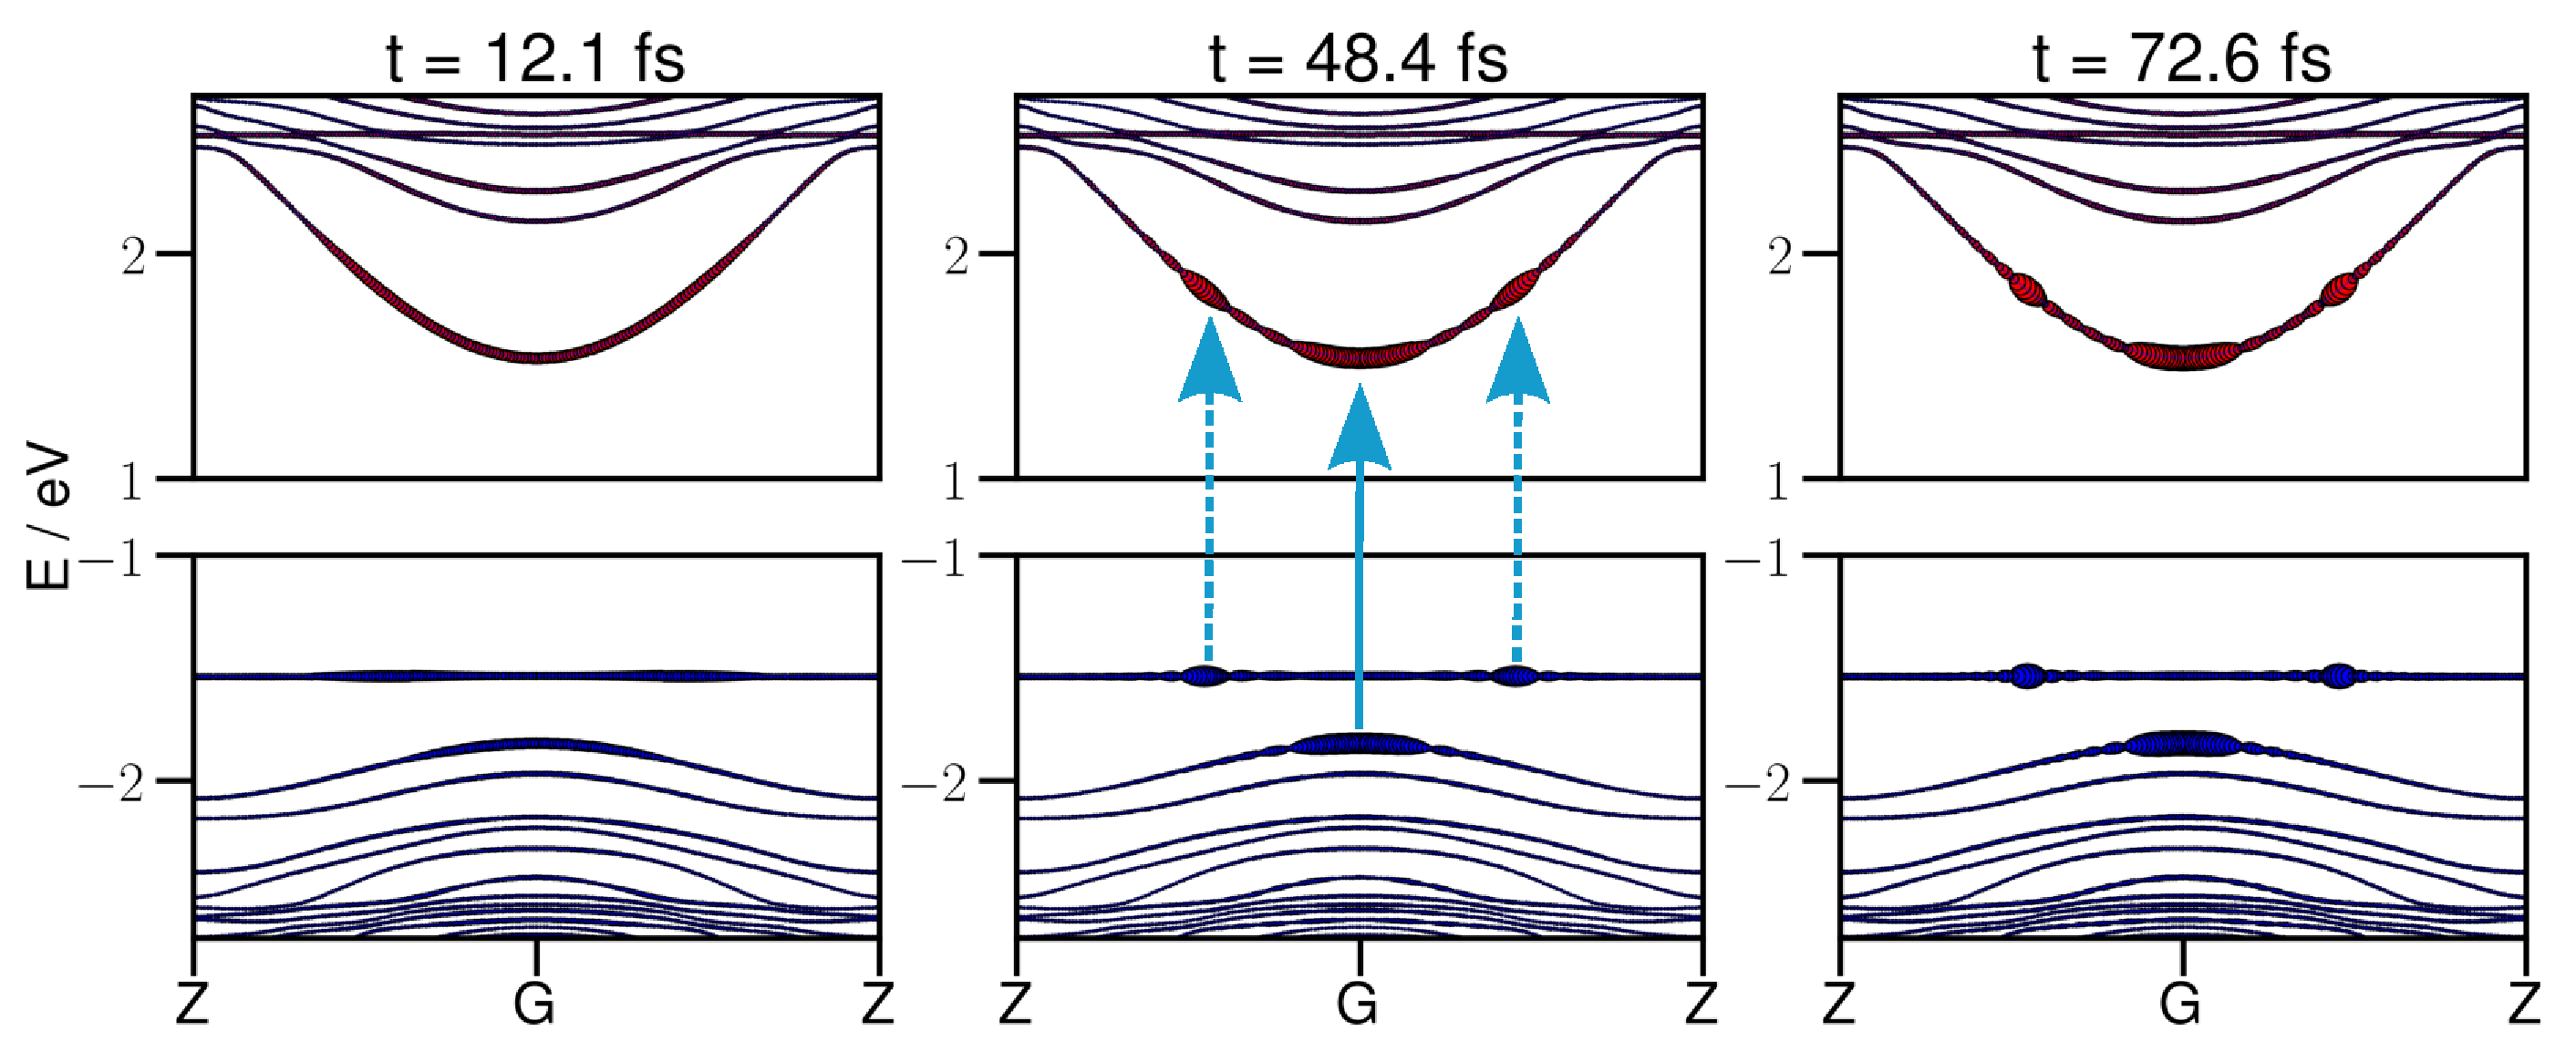
\includegraphics[height=6cm]{cap5/fig/dynpop_3.38_cut.eps}
\caption{ ({\bf Arriba}) izquierda: espectro de absorción para C$_1$, cat aislado y nw$_1$ aislado y  derecha: cargas en función del tiempo perturbando el sistema con un láser de $3.38$ eV. ({\bf Abajo}) Estructura de bandas de C$_1$. Sobre las bandas se grafica la diferencia de población electrónica que se genera al iluminar C$_1$ con el láser a 3 tiempos distintos: en azul se representa la disminución de la población electrónica al iluminar y en rojo el aumento de la población electrónica al iluminar con el láser.}
\label{ilu_3.38}
\end{figure}


Al iluminar C$_1$ con un láser seteado con la energía del máximo de absorción de la segunda banda, es decir a $3.38$ eV (ver figura \ref{ilu_3.38}) no se observa transferencia de carga entre CAT y el nw aunque las transiciones estén presentes tal como lo indica el espectro. Para entender este hecho nos remitimos a los gráficos de $\Delta P$ sobre las bandas, en el cual observamos varias transiciones: a) una transición en G que ocurre entre la b$_b$ y b$_1$, ambas bandas con contribuciones del nw$_1$ (fijarse figura \ref{dos_bandas_spec} (1) y (2)) y b) 2 transiciones una a cada lado de G, entre G y el punto crítico Z que ocurren entre la b$_a$ y b$_1$. En este último caso, las mismas provienen de las excitaciones que se produjeron en el máximo de absorción de la banda de menos energía ($3.08$ eV). La transición en G no contribuye a la transferencia de carga ya que se da entre 2 bandas con mayores contribuciones por parte del nw$_1$ mientras que las otras dos transiciones si contribuyen como se observó en la iluminación anterior. La resultante de las transiciones que ocurren da como resultado final la ausencia de la transferencia de carga. 


%VER ESTA PARTE%

%En general, las bandas que se observan en el espectro son el resultado de las transiciones que ocurren de acuerdo a la ecuación \ref{eq:prob_osc_final} la cual señala que la probabilidad de la transición está directamente relacionada con la integral de $F(t,w)$ entonces calculando el área bajo la curva de esta función centrada en w$_{fi}$ podemos justificar los resultados obtenidos por dftb+ utilizando la regla de oro de fermi.


%Las transiciones no necesariamente generan transferencia de carga, de acuerdo a los gráficos de $F(w,t)$ (figura \ref{fermi_F}) la probabilidad de transición es mayor en w$_{fi}$ y por ende las excitaciones que ocurren en G deberían a priori tener mayor peso con respecto a otras como se observa en las iluminaciones a $3.08$ eV y $3.38$ eV. Sin embargo, cuando la energía del láser es mayor se observan cada vez más transiciones en otros {\bf k} y por lo tanto las mismas van ganan más peso o igualan a las que ocurren en G. En estos casos, se observa transferencia de carga cuando predominan excitaciones que involucren la b$_a$ que es la banda del colorante y otra banda con contribuciones del nw.


\begin{figure}[!htb]
\centering
\includegraphics[height=17cm]{cap5/fig/ultimas_dynpop.eps}
\caption{Gráficos de: ({\bf izquierda}) estructura de bandas de C$_1$ y $\Delta P$ que se genera al iluminar el sistema con E$_{laser}$ de $3.50$ eV, $3.70$ eV, $3.83$ eV y $3.97$ eV a 3 tiempos distintos: en azul $\Delta P - $ y en rojo $\Delta P + $ donde las flechas punteadas representan las nuevas transiciones y ({\bf derecha}) cargas de Mulliken en función del tiempo correspondientes a cada una de las E$_{laser}$ utilizadas.}
\label{ilu_todas}
\end{figure}


En la figura \ref{ilu_todas} se muestran las evoluciones temporales de las poblaciones (izquierda) y de las cargas de Mulliken (derecha) para las iluminaciones a $3.50$ eV, $3.70$ eV, $3.83$ eV y $3.97$ eV. A medida que aumenta la energía de la irradiación, se observan por un lado nuevas transiciones y por otro, que las excitaciones que provienen de las bandas de menor energía se van acercando cada vez más al punto crítico Z y se alejan de G (fijarse en las flechas celestes). De los cálculos realizados, sólo se observa transferencia de carga para $3.08$ eV, $3.83$ eV y $3.87$ eV, particularmente en $3.83$ eV se transfiere mayor carga con respecto al resto. Si bien en las irradiaciones más energéticas analizadas hay mayores contribuciones para que la transferencia ocurra, en $3.97$ eV aparece una nueva excitación entre 2 bandas con aportes predominantes del nw disminuyendo el resultado final. Es importante recalcar que todas las flechas que representan las excitaciones entre bandas tienen la misma longitud, entonces asignando solo una transición podemos mover la flecha y predecir todas las transiciones que ocurren. Este procedimiento ayuda principalmente al investigar iluminaciones a mayores energías en donde el proceso de asignación es engorroso. 


\section{Conclusiones}

En este capítulo se utilizó como herramienta el código dftb+ para calcular propiedades del estado fundamental y del estado excitado de sistemas CAT + nw. El hecho de utilizar distintos cubrimientos de catecol en la superficie del nw se ve reflejado en todos los resultados obtenidos. Los sistemas de mayor cubrimiento C$_1$ y C$_2$ presentan una estabilidad adicional respecto a los demás complejos debido a la deslocalización de los OM a lo largo del nw producto de la corta distancia entre moléculas de catecol de celdas unidad contiguas. La estabilización se ve reflejada en la dispersión de la estructura de bandas y en los valores de E$_ad$.

Los complejos CAT-nw de ZnO muestran bandas de absorción en la zona del visible lo cual no ocurría cuando el colorante y el nw se encontraban aislados. La aparición de esas bandas se debe principalmente a las interacciones que ocurren entre el SC y al catecol, en donde este último se corresponde con colorantes tipo II. 

Cuando analizamos C$_1$ particularmente, se llega a la conclusión de que la evolución temporal de las poblaciones al iluminar el sistema con un láser responde a la regla de oro de Fermi. También se observa que cada banda en el espectro de absorción del complejo es el resultado de muchas transiciones y que solo se aprecia transferencia de carga cuando al iluminar predominan transiciones que ocurren desde bandas con mayores aportes del colorante a bandas con mayores aportes del nw.


  %\chapter{Propiedades catalíticas de nw de ZnO wurtzita.}

Hoy en día, las caldas solares sensibilizadas por colorante (DSSC) son los sistemas más investigados para la conversión de energía solar en electricidad, particularmente para su implementación en dispositivos donde se requieren bajos costos y buen rendimiento. Las DSSC de mayor rendimiento utilizan electrolitos líquidos a base de disolventes orgánicos, los cuales tienen el inconveniente de una alta presión de vapor y un severo impacto medioambiental. Además, varios disolventes orgánicos son tóxicos y/o explosivos, lo que limita seriamente sus aplicaciones prácticas en DSSC debido a problemas de seguridad. A pesar de que se han propuesto varias alternativas a los disolventes orgánicos \cite{Li2014,Pringle2013}, el problema que a veces se ignora es la contaminación de la celda por medio de humedad/agua que afecta tanto al rendimiento de la celda como a la estabilidad a largo plazo. De hecho, siempre están presentes trazas de agua en la solución electrolítica y en los poros/huecos de la película del electrodo SC, que eventualmente se introducen durante el ensamblaje de la celda o al operar en condiciones ambientales. En consecuencia, es fundamental averiguar cual es el papel específico del agua como componente en las DSSC, si se trata de un envenenamiento o la palabra clave para el éxito, lo cual se logra a partir del análisis minucioso de todos los fenómenos establecidos en el medio acuoso. Entonces, consideramos muy interesante y sorprendente el hecho de que, en los últimos años, la comunidad científica ha orientado sus investigaciones en dirección a las DSSC fabricados con electrolitos a base de agua, haciendo estudios tanto experimentales \cite{Husmann2018,Cassone2018} como teóricos con TD-DFT \cite{Angelis2011}. De esta manera se podrían lograr fácilmente costos reducidos, no inflamabilidad, volatilidad reducida y compatibilidad ambiental mejorada. Las modificaciones de fotoanodos, la introducción de nuevos aditivos y tensioactivos, la selección de pares redox específicamente concebidos, la preparación de cátodos adecuados y la estabilización de electrolitos han conducido progresivamente a la fabricación de DSSC 100$\%$ acuosas ({\bf DSSC acuosas}, ver figura \ref{dssc_acuosa}). Lograr un alto rendimiento en una celda completamente acuosa representa un avance significativo para las DSSC y devuelve la atención a su propósito inicial: la realización de un sistema fotosintético artificial capaz de convertir la energía de la luz solar visible en electricidad, mediante el uso de un disolvente único, agua, el solvente de la vida. Por último y no menos importante el uso del agua como componente clave puede representar un gran paso hacia su amplia difusión en el mercado. 



\begin{figure}[!htb]
\centering
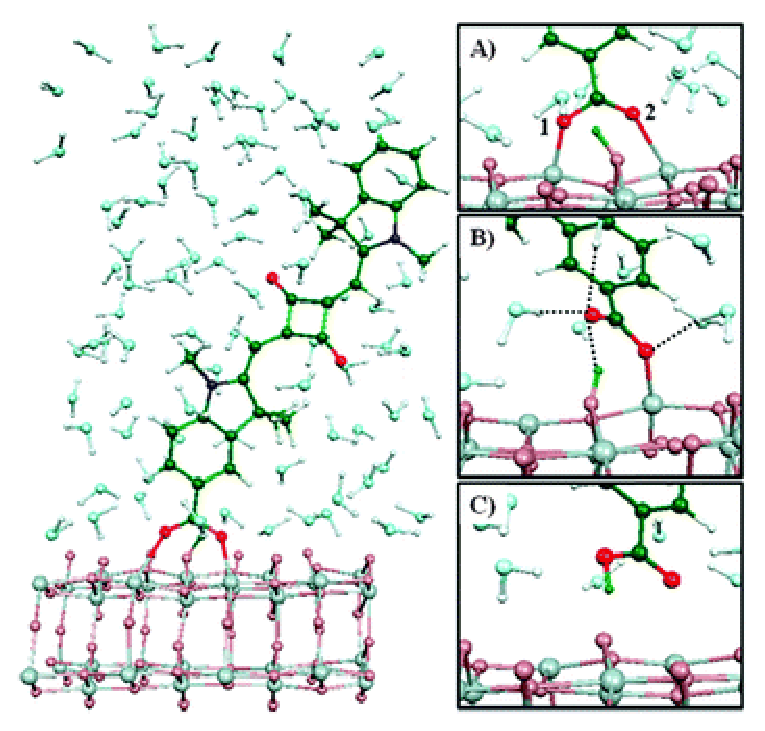
\includegraphics[height=6cm]{cap6/figs/dssc_acuosa.eps}
\caption{Imagen de una DSSC aquosa: Squaraina adsorbida sobre un slab de anatasa, rodeada por 90 moléculas de agua. En las imágenes del lado derecho, se muestran las configuraciones relevantes muestreadas durante el estudio TD-DFT: A) configuración inicial bidentada con átomos de oxígeno etiquetados, B) configuración monodentada y C) colorante disociado. Las líneas punteadas en B) representan enlaces de hidrógeno al grupo carboxílico. Extraído de \cite{Angelis2011}} 
\label{dssc_acuosa}
\end{figure}



De acuerdo al trabajo publicado por Bella \textit{et al} \cite{Bella2015}, parece que la calidad de la interfase fotoanodo/electrolito afecta negativamente la eficiencia de las DSSC acuosas en comparación con las basadas en disolventes orgánicos. La hidrofilicidad excesiva de la superficie sensibilizada con el colorante favorece la desorción de la molécula sensibilizadora disminuyendo así la fotocorriente y la estabilidad en el tiempo; por otro lado, los colorantes altamente hidrófobos no permiten la humectabilidad completa del electrodo lo que, a su vez, da como resultado un proceso de regeneración menos efectivo para los electrolitos acuosos. Las estrategias más efectivas hacia DSSC acuosas realistas incluyen el uso de complejos de cobalto como mediadores redox, colorantes hidrófobos combinados/funcionalizados con tensioactivos o débilmente hidrófilos obtenidos mediante la modificación de sensibilizadores ya disponibles y contraelectrodos tolerantes al agua con una amplia superficie. Sin embargo, el estudio de las DSSC acuosas se encuentra en una etapa temprana y aún faltan estudios comparativos que puedan mejorar en gran medida el conocimiento de estos sistemas.

El objetivo de este capítulo es estudiar al agua como componente electrolítico en sistemas agua - nw de ZnO wurtzita y las interacciones que ocurren entre ambas especies utilizando distintos niveles de teoría: dinámica molecular (LAMMPS), DFT (Quantum expresso) y DFTB (dftb+). 


\section{Complejos 1H$_2$O + nw ZnO wurtzita}

En primer lugar se realizaron simulaciones de sistemas nw-H$_2$O utilizando solamente 1 molécula de agua. Las superceldas que se utilizaron en los cálculos son las que se muestran en la figura \ref{supercelda}, las cuales se construyeron apilando 2 celdad unidad o 2 nw$_1$ en el eje z. Es importante aclarar que las estructuras de celda unidad son las mismas que utilizamos en el capítulo 5. El tamaño de la supercelda debe ser lo suficientemente grande como para que la molécula de agua no interaccione con su imagen periódica y además el costo computacional no sea muy elevado especialmente al utilizar Quantum Espresso (\textbf {QE}).

La molécula de agua se puede unir a la superficie del nw de diversas maneras. En esta tesis propusimos 2 configuraciones: C$_A$ y C$_B$ (ver figura \ref{supercelda}), en C$_A$ el O del agua interacciona con un Zn superficial del nw (O$_w$--Zn$_{nw}$) mientras que en C$_B$ uno de los H del agua interacciona con un O superficial del nw (H$_w$--O$_{nw}$). Ambos Zn y O superficiales tienen número de coordinación 3 lo que los vuelve más reactivos con respecto a los otros átomos que se encuentran dentro del nw con número de coordinación 4. 


\begin{figure}[!htb]
\centering
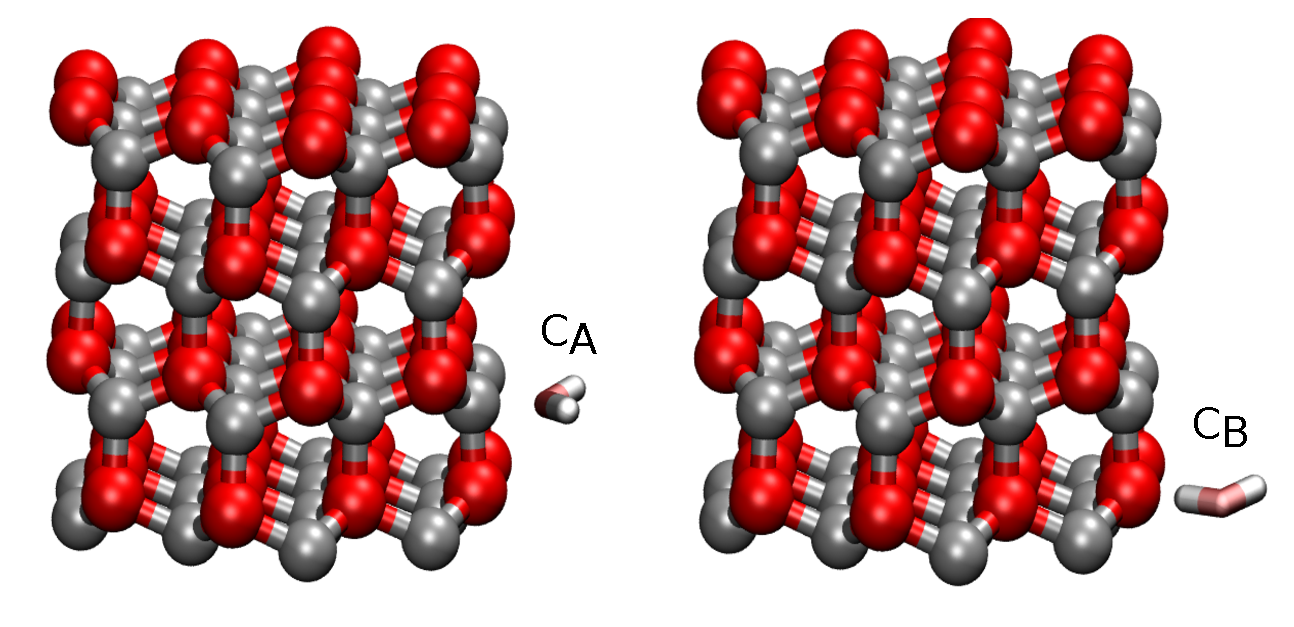
\includegraphics[height=5cm]{cap6/figs/conf_ca_cb.eps}
\caption{Superceldas utilizadas para los cálculos. C$_A$ y C$_B$ son las configuraciones propuestas para la unión del agua a la sueprficie del nw.} 
\label{supercelda}
\end{figure}


\subsection{Análisis configuracional}

Ambos sistemas con distinta configuración del agua fueron relajados utilizando LAMMPS, QE y dftb+. 
Se utilizó el potencial ReaxFF para los cálculos realizados con el software LAMMPS ya que según la literatura se han encontrado buenos resultados en concordancia con los experimentos y el pseudopotencial pbe en QE. 


Una manera típica de buscar mínimos estables es simplemente relajando desde las distintas configuraciones. Sin embargo, antes de realizar este procedimiento decidimos dejar que la dinámica molecular (DM), a través de LAMMPS, pruebe varias configuraciones hasta quedarse con la más estable a medida que disminuye la temperatura. En este método que se llama \textbf{templado simulado}, el sistema explora la superficie de energía potencial y a medida que disminuye la temperatura se va ubicando en mínimos locales. De esta manera, al llegar a aproximadamente 0 K, el sistema se encuentra en un mínimo que puede ser el mínimo global o un mínimo local muy estable. El gráfico de la figura \ref{rampa} muestra la rampa de temperatura (300 K-$0.05$ K) que se utilizó para el templado a medida que avanza la dinámica. 


\begin{figure}[!htb]
\centering
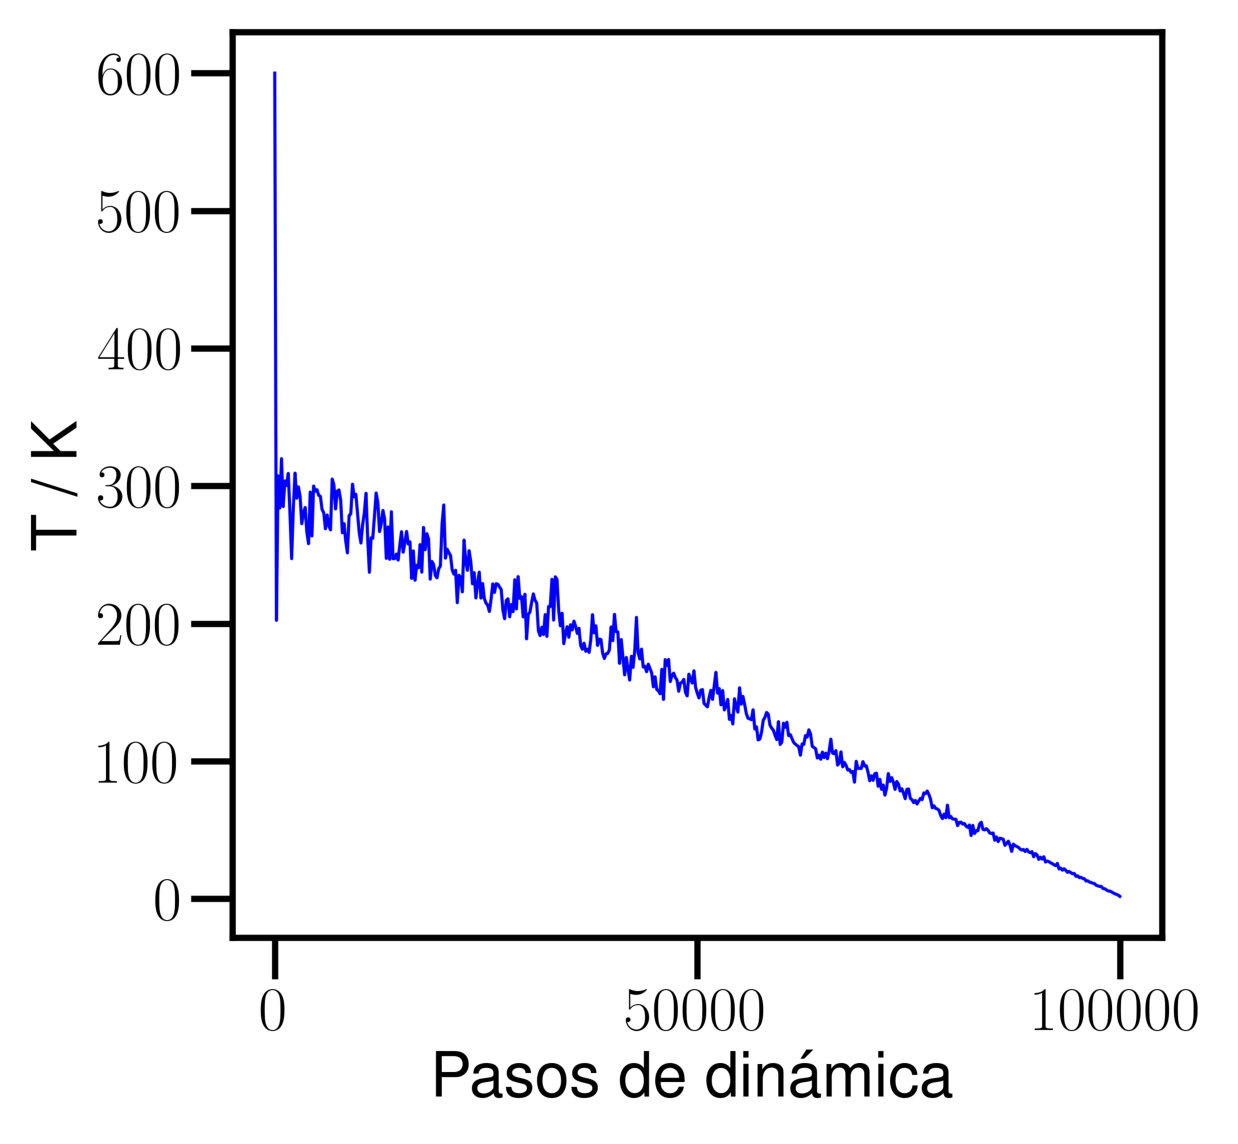
\includegraphics[height=8cm]{cap6/figs/temps_steps.eps}
\caption{Gráfico de temperatura vs pasos de dinámica para la relajación de C$_A$ y C$_B$ en LAMMPS utilizando templado simulado} 
\label{rampa}
\end{figure}

Luego del templado simulado se realiza una relajación en z a 0 K con LAMMPS. Las configuraciones obtenidas con dinámica molecular fueron relajadas nuevamente por dftb+ y QE, respectivamente en z a 0 K. Los resultados obtenidos de las optimizaciones de geometría se muestran en la figura \ref{relax}. 


\begin{figure}[!htb]
\centering
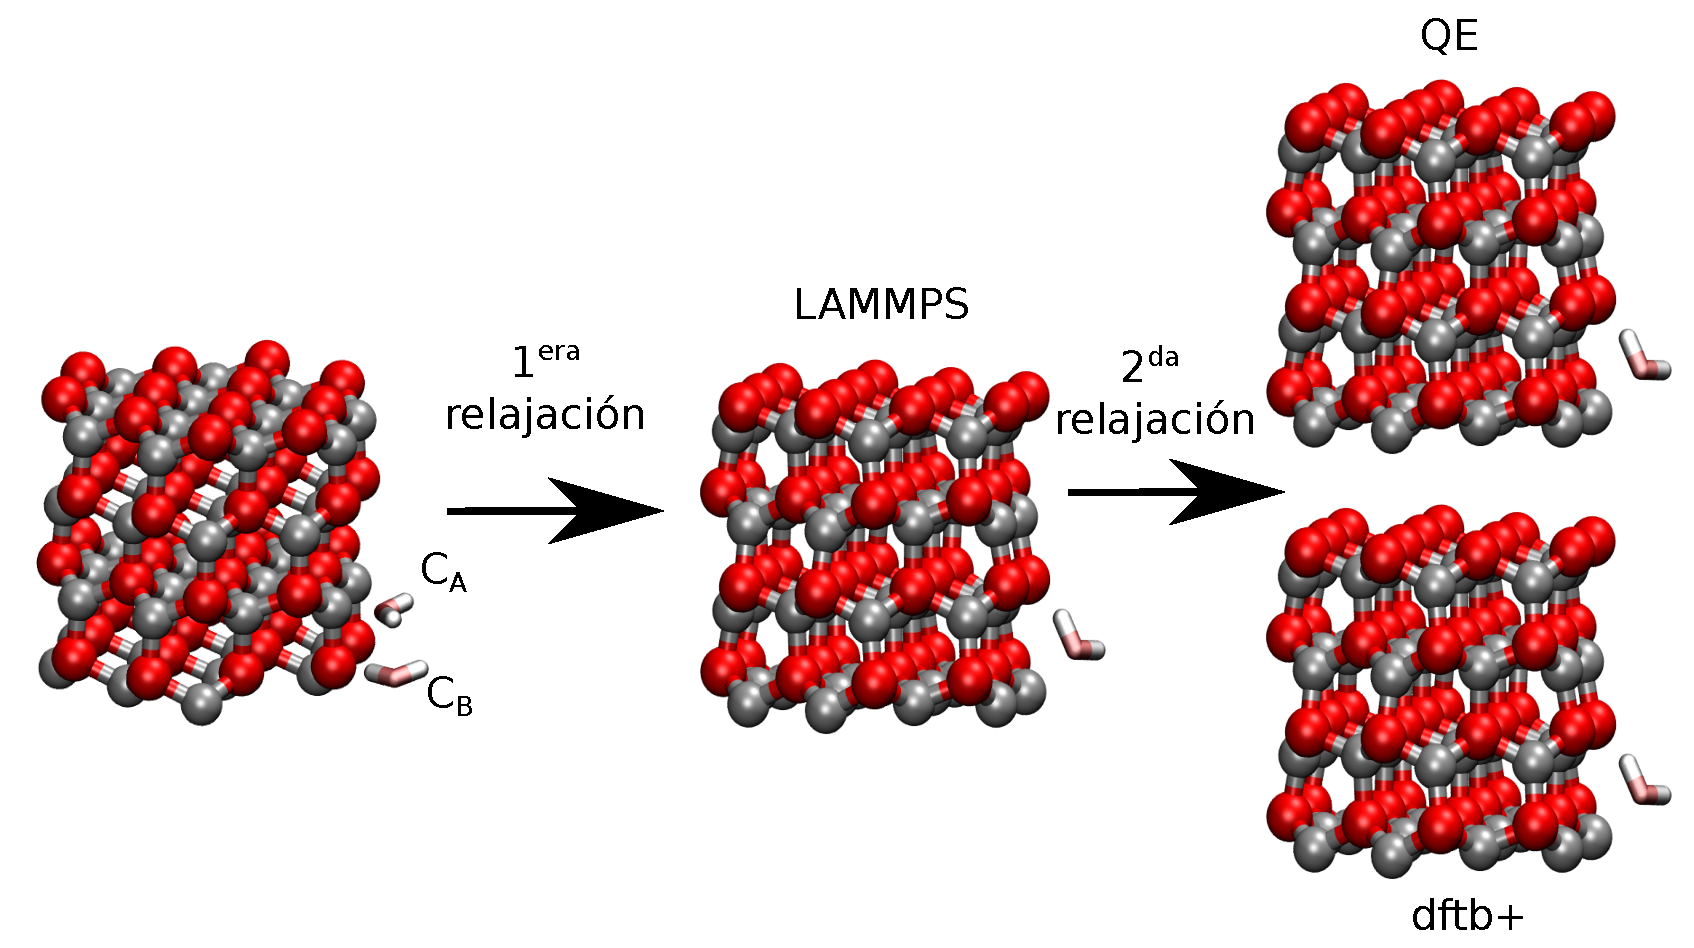
\includegraphics[height=8.5cm]{cap6/figs/relax.eps}
\caption{Relajaciones de las configuraciones C$_A$ y C$_B$ utilizando primero LAMMPS y luego QE y dftb+ } 
\label{relax}
\end{figure}

La relajación con DM para los sistemas C$_A$ y C$_B$, respectivamente, dio como resultado dos configuraciones idénticas y distintas con respecto a C$_A$ y C$_B$. Luego al relajar por segunda vez con QE y con dftb+ se obtuvo una estructura prácticamente igual a la que encontró LAMMPS como lo demuestra a simple vista la figura \ref{relax}. Para corroborar la hipótesis de que los tres métodos encontraron la misma configuración más estable para el sistema 1H$_2$0-nw, se compararon por un lado los diámetros y alturas de las celdas unidad del nw y por otro las distancias H$_w$--O$_{nw}$ y Zn$_{nw}$--O$_w$ que muestran el posicionamiento de las moléculas de agua con respecto al nw. Todas las mediciones se realizaron para cada una de las estructuras obtenidas luego de las relajaciones con los distintos software.

\begin{table}[!htb]
  \caption{Comparación de diámetro y altura de las celdas unidad de los sistemas 1H$_2$0-nw relajados en z utilizando LAMMPS, dftb+ y QE}
  \label{tabla_distancias_nw}
  \centering
  %\resizebox{14cm}{!} {
  \begin{tabular}{ c  c  c  }
   \hline
   \multicolumn{1}{c}{} & \multicolumn{1}{c}{Diámetro ({\AA})} & \multicolumn{1}{c}{Altura ({\AA})} \\
   \hline
    LAMMPS & $9.80$ & $5.47$\\
    dftb+ & $9.98$ & $5.46$\\ 
    QE & $9.88$ & $5.40$\\ 
    \hline
 \end{tabular}
 %}
  \end{table}

La tabla \ref{tabla_distancias_nw} compara solo las estructuras de los nw de los sistemas 1H$_2$0-nw. Los valores obtenidos con QE son tomados como referencia ya que los cálculos con DFT han demostrado tener una buena concordancia con resultados experimentales para sistemas SC??. De acuerdo a esta expresión, las 3 estructuras de nw pueden considerarse equivalentes debido a que el diámetro y la altura de las celdas unidad obtenidas con dftb+ y LAMMPS difieren en menos de $0.2$ {\AA} con respecto a QE, error que se considera razonable. Los valores de diámetro que arroja LAMMPS son más próximos a la referencia en comparación con dftb+ mientras que este último muestra valores de altura de la celda unidad más cercanos a QE. 


\begin{figure}[!htb]
\centering
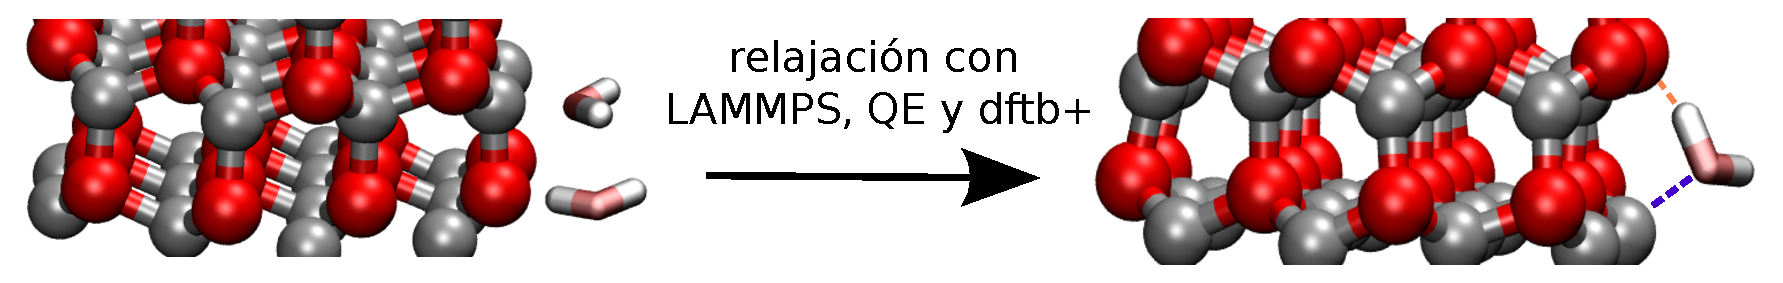
\includegraphics[height=2.1cm]{cap6/figs/antes_despues_relax_cur.eps}
\caption{(\textbf {Izquierda}) configuraciones iniciales (C$_A$-C$_B$) y (\textbf {derecha}) configuración final en todos los casos (C$_C$)} 
\label{CC}
\end{figure} 

\begin{table}[!htb]
 \caption{Comparación de las distancias H$_w$--O$_{nw}$ y Zn$_{nw}$--O$_w$ de los sistemas 1H$_2$0-nw relajados con LAMMPS, dftb+ y QE}
 \label{tabla_distancias_agua}
 \centering
 %\resizebox{14cm}{!} {
 \begin{tabular}{ c  c  c  }
  \hline
  \multicolumn{1}{c}{} & \multicolumn{1}{c}{Distancia \textcolor{orange}{\textbf{H}}$_w$--\textcolor{orange}{\textbf{O}}$_{nw}$ ({\AA})} & \multicolumn{1}{c}{Distancia \textcolor{blue}{\textbf{Zn}}$_{nw}$--\textcolor{blue}{\textbf{O}}$_w$ ({\AA})} \\
  \hline
    LAMMPS & $1.56$ & $2.30$\\
    dftb+ & $1.78$ & $2.13$\\ 
    QE & $1.64$ & $2.12$\\ 
    \hline
 \end{tabular}
 %}
\end{table} 
  
La tabla \ref{tabla_distancias_agua} compara las distancias H$_w$--O$_{nw}$ y Zn$_{nw}$--O$_w$ para los sistemas 1H$_2$0-nw optimizados utilizando tres niveles de teoría. En este caos tampoco se observa una tendencia en los valores obtenidos, sin embargo, las diferencias con respecto a QE también son menores a $0.2$ eV. Podemos decir, entonces, que las tres estructuras obtenidas de las relajaciones de C$_A$ y C$_B$ con distintos software son equivalentes entre si, lo cual significa que los métodos conciden en que la configuración del sistema 1H$_2$0-nw ZnO más estable es la que se muestra en la figura \ref{CC} (C$_C$).
Los resultados nos permiten validar los métodos LAMMPS y dftb+ en cuestión, otorgando credibilidad a los cálculos de relajación en sistemas H$_2$0-nw ZnO. Por otro lado observamos que la configuración mas estable encontrada por los 3 software tiene en cuenta ambas interacciones simultáneamente, es decir:  H$_w$-O$_{nw}$ y Zn$_{nw}$-O$_w$, en lugar de considerar las interacciones por separado como planteamos al inicio del capítulo.

En último lugar, para investigar el tipo de unión que que se establece entre el adsorbato (agua) y la superficie del SC (nw) realizamos cálculos de energía de adsorción, E$_ad$, para la configuración C$_C$ (ver tabla \ref{tabla_ead})

La E$_{ad}$ se obtuvo de acuerdo a la siguiente ecuación:

\begin{equation}
 E_{ad} = E_{T(H_20 + nw)} - E_{T(nw)} - E_{T(H_20)}
\end{equation}

donde E$_{T(H_20 + nw)}$ es la energía total del sistema 1H$_2$0-nw, E$_{T(nw)}$ la energía total del nw de ZnO y E$_{T(H_20)}$ de la molécula de agua. 

  
\begin{table}[!htb]
  \caption{Energías de adsorción para C$_C$ calculadas mediante los 3 métodos analizados}
  \label{tabla_ead}
  \centering
  \begin{tabular}{ c  c }
   \hline
   \multicolumn{1}{c}{} & \multicolumn{1}{c}{E$_{ad}$ (eV)}\\
   \hline
   & C$_C$\\
   \hline
    LAMMPS & $-1.02$ \\
    dftb+ & $-1.15$ \\ 
    QE & $-0.81$ \\
    \hline
   \end{tabular}
\end{table}  
  
Se observan valores negativos de E$_{ad}$ para las 3 simulaciones, reflejando una unión fuerte entre el adsorbato (H$_2$O) y el adsorbente (nw). Tomando a QE como el método más preciso, dftb+ y LAMMPS sobrestiman la interacción H$_2$O-nw. 
  
  
\section{Complejos nH$_2$O + nw ZnO wurtzita}

En esta sección se realizó en primer lugar un cálculo de DM para el sistema: nw de ZnO wurtzita + primer cilindro de solvatación de agua (\textbf {1slv agua-nw}) a 300 K.  El 1$^{er}$ cilindro de solvatación se seleccionó realizando un corte a una distancia de $2.33$ {\AA} desde la superficie del alambre en dirección radial de acuerdo al gráfico de la función de distribución radial \textbf{g(r)} (ver figura \ref{dist_radial}). Por definición sabemos que g(r) es la probabilidad de hallar una partícula a una distancia dada de otra partícula/superficie/etc. comparada con la probabilidad de una distribución aleatoria de igual densidad. Entonces, resulta interesante observar que g(r) nos brinda información acerca de como están orientados los átomos de las moléculas de agua, en este caso hay una gran probabilidad de encontrar H a una distancia de $1.00$ {\AA} de la superficie del nw y recién a $2.1$ {\AA} los átomos de O. La pequeña distancia entre el O del nw y el H del agua indica la formación de un enlace entre ambas especies.


%$g(r)$ = probabilidad de hallar una partícula a una distancia dada de otra partícula/superficie/etc. comparada con la probabilidad de una distribución aleatoria de igual densidad. 

%* Estructuración hasta 7 Å - 8 Å 
%* Orientación de los H del agua

\begin{figure}[h!]
\centering
\includegraphics[height=5cm]{cap6/figs/gr-O-H.eps}
\caption{Distribución radial de agua en presencia del nw de ZnO.} 
\label{dist_radial}
\end{figure}


Como supercelda para la simulación en LAMMPS a 300 K se utilizaron 5 celdas unidad de nw apiladas en el eje z tal como se muestra en la figura \ref{1_esfera} a la derecha. La altura fue seleccionada con el objetivo de no forzar una configuración ficticia del agua favorecida por interacciones (puente hidrógeno, por ejemplo) entre celdas vecinas. 



\begin{figure}[h!]
\centering
\includegraphics[height=8cm]{cap6/figs/1_esfera_a.eps}
\caption{Dinámica en LAMMPS a 300 K para el sistema 1slv agua-nw.} 
\label{1_esfera}
\end{figure} 

La figura \ref{1_esfera} muestra la estructura obtenida luego del cálculo a 300 K con LAMMPS. En la misma se observa que algunas moléculas de agua cuentan con la energía suficiente para romper uno de los enlaces H-O y en consecuencia los H disociados forman un nuevo enlace con los O superficiales tricoordinados del nw. Mientras la disociación de una molécula de agua ocurre se genera un ión OH$^-$ y a su vez otra molécula de agua vecina se acerca para conservar el orden de enlace ayudando a que el proceso ocurra (ver círculo violeta de la figura \ref{1_esfera}). 

Los resultados obtenidos con la DM corrobora la hipótesis planteada al analizar la g(r) ya que los H que se muestran a 1 {\AA} son los átomos que se disocian de las moléculas de agua y forman enlace con la superficie del nw. 


\subsection{Catálisis de agua sobre nw de ZnO wurtzita}

La disociación del agua sobre el nw de ZnO propuesta por LAMMPS debe ser verificada por otro método teórico. En este caso utilizamos DFT (QE) como herramienta ab-initio para la validación de este resultado. Desde el punto de vista experimental, ya se han observado disocia


Se realizó un cálculo de CNEB (Climbing Nudget Elastic Band) en QE para la disociación del agua utilizando como estado inicial la estructura con el agua sin disociar y como estado final la estructura con el agua disociada. Es importante recalcar que ambos estados fueron previamente relajados con QE, asegurándonos de la estabilidad de ambos.   


A la derecha de la imagen se muestra un gráfico de energía en función de la coordenada de reacción para las 7 imágenes que utilizó CNEB para encontrar el camino de reacción de mínima energía. 
    
    
    
\subsection{Complejos 1slv agua-nw utilizando nw con distintos diámetros}

Con el objetivo de realizar un análisis cuantitativo de la disociación de agua sobre nw se realizaron cálculos de DM a 300 K con LAMMPS en sistemas 1slv agua-nw utilizando nw de distinto diámetro: nw$_{d1}$, nw$_{d2}$, nw$_{d3}$, nw$_{d4}$ y nw$_{d5}$ (ver figura \ref{anchos}). 

Con los resultados obtenidos en las simulaciones se realizó la figura \ref{anchos_dis}, la cual muestra dos gráficos de proporción de disociación de agua en función del tiempo en ps. La proporción mencionada se calcula como la relación entre cantidad de disociaciones que ocurren y la cantidad de disociaciones posibles. Es importante mencionar también que cada curva graficada es el promedio de 3 cálculos con distinta semilla. 


\begin{figure}[h!]
\centering
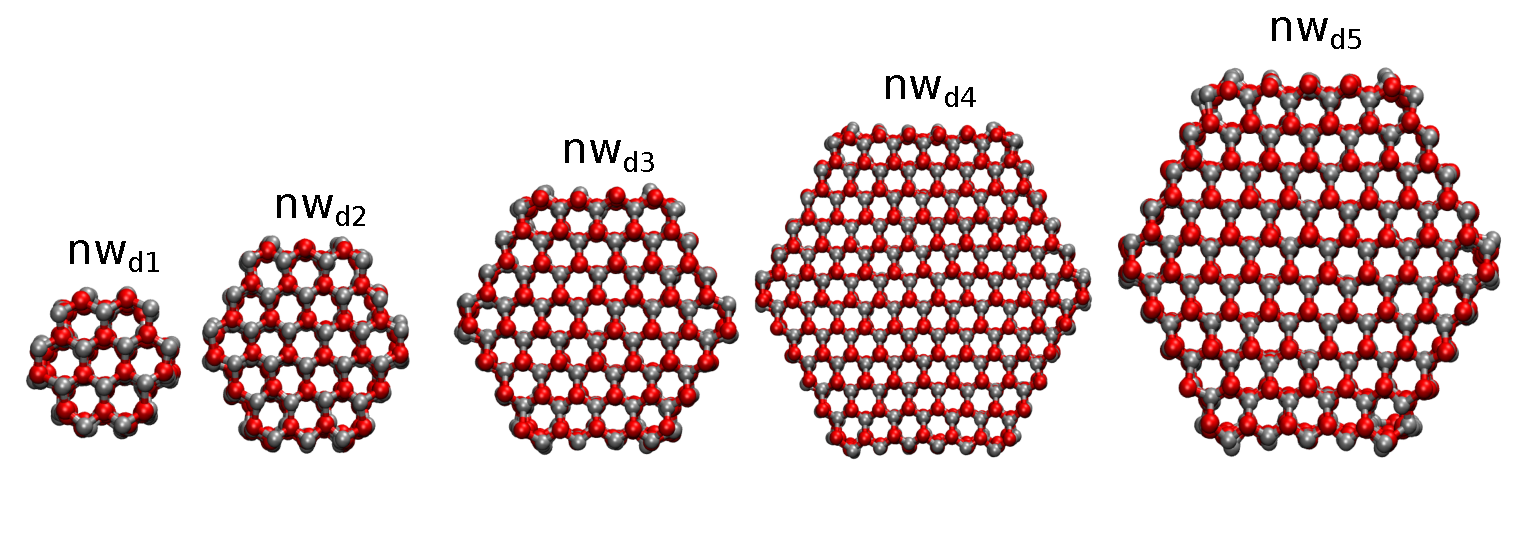
\includegraphics[height=5cm]{cap6/figs/anchos.eps}
\caption{Nw luego de realizar simulaciones de sistemas 1slv agua-nw con LAMMPS a 300 K. Los diámetros para cada nw son: $10.48$ {\AA} (nw$_{d1}$), $16.99$ (nw$_{d2}$), $23.36$ {\AA} (nw$_{d3}$), $30.33$ {\AA} (nw$_{d4}$) y $36.79$ {\AA} nw$_{d5}$.} 
\label{anchos}
\end{figure}



\begin{figure}[h!]
\centering
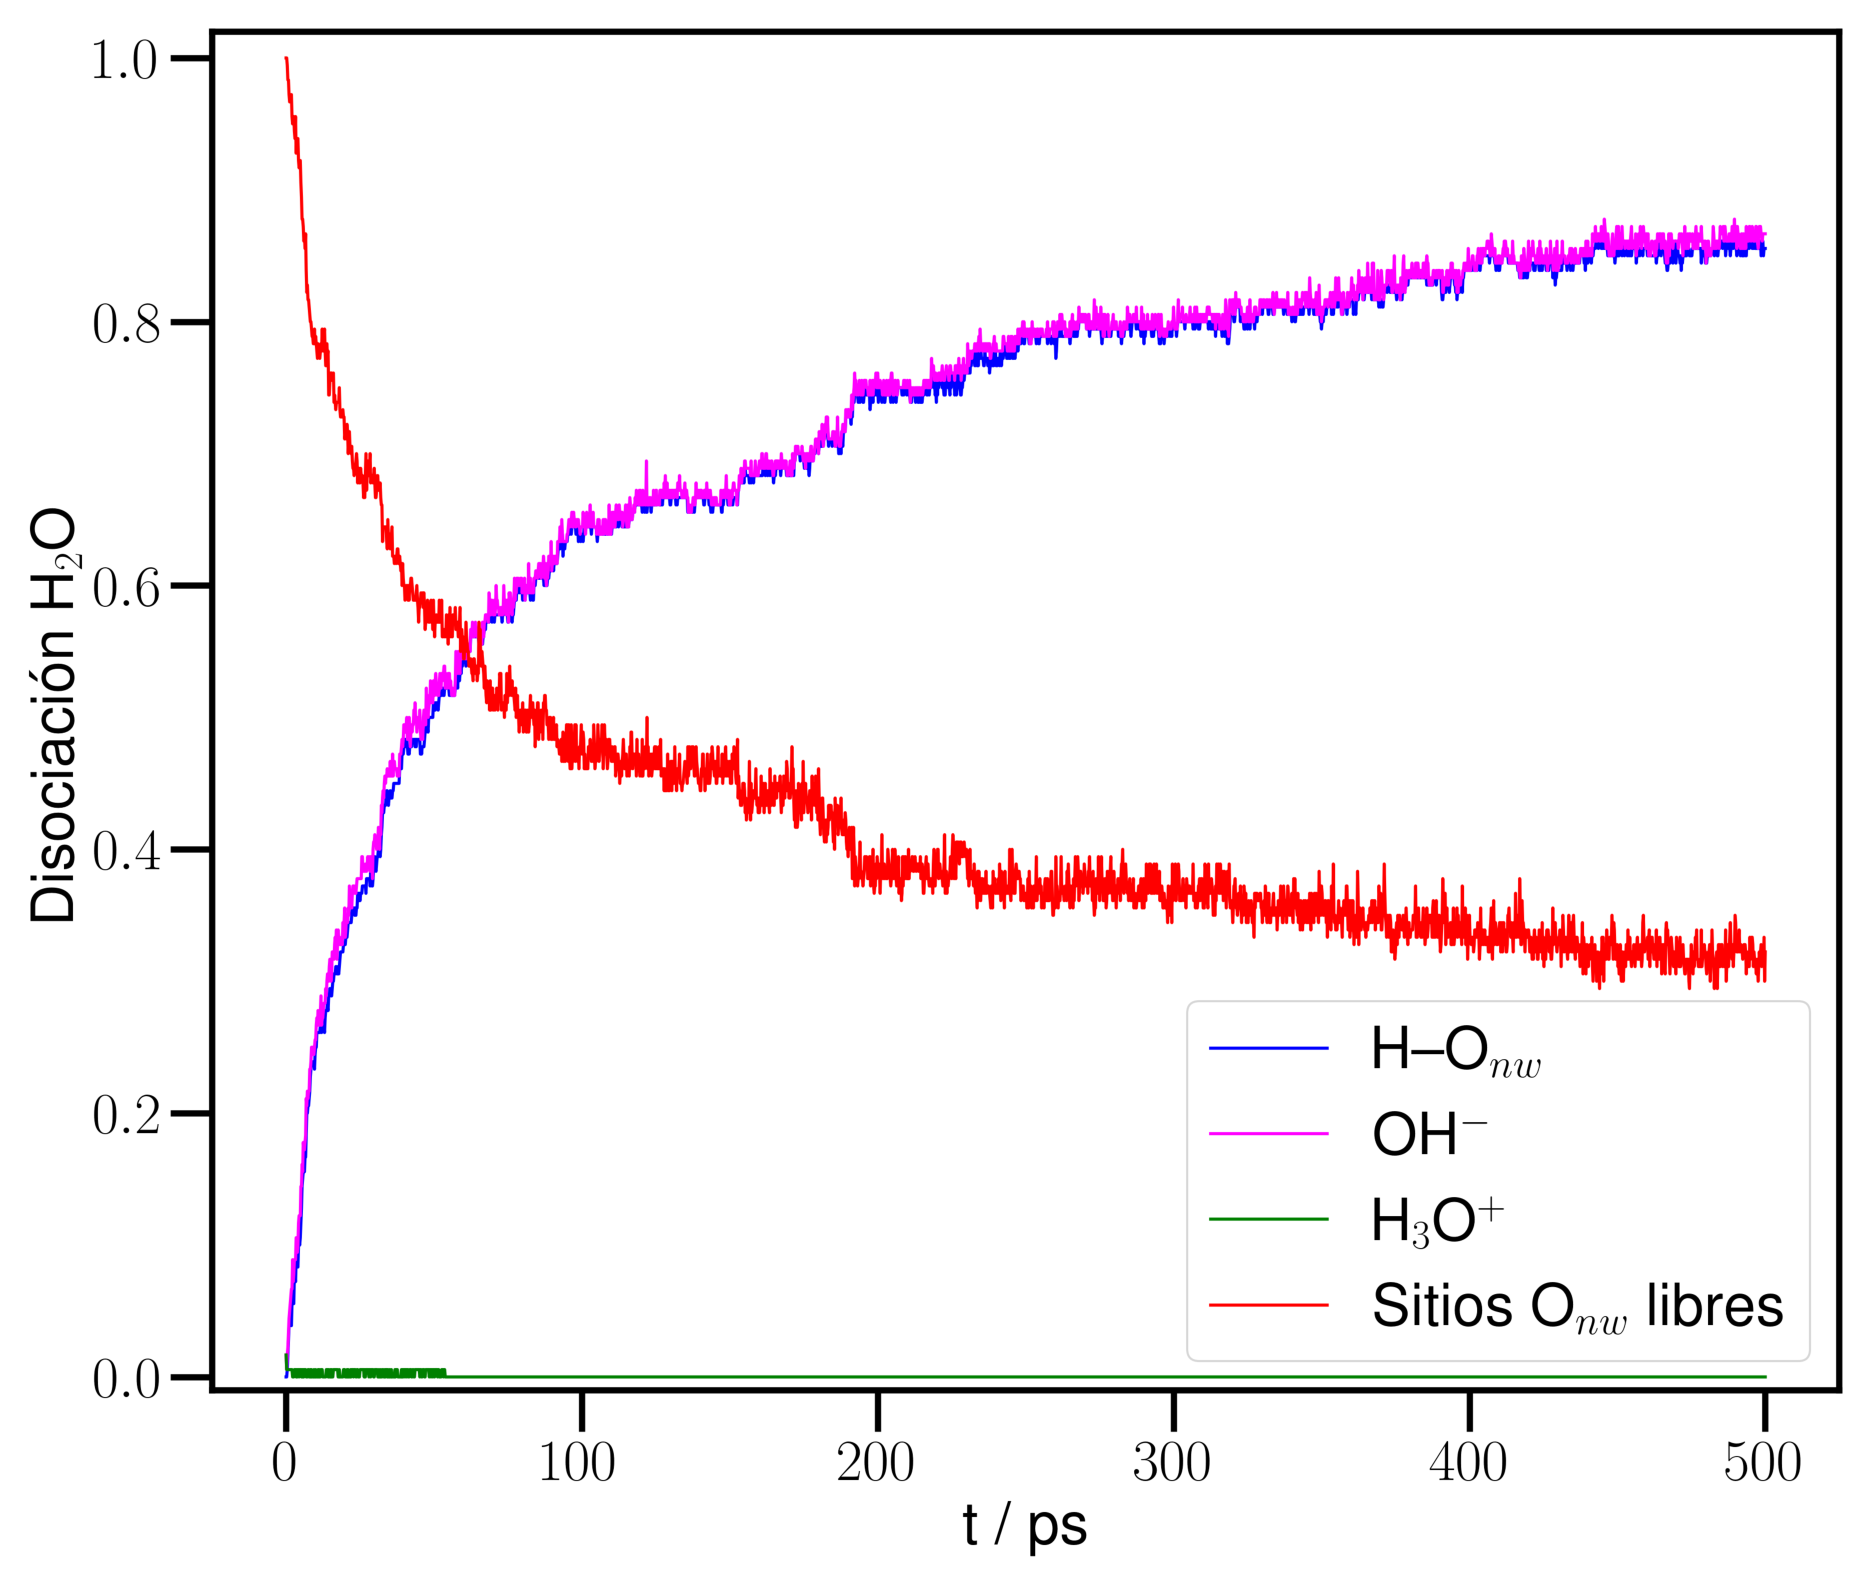
\includegraphics[height=6cm]{cap6/figs/prom_1.eps}
\includegraphics[height=6cm]{cap6/figs/comparacion_anchos.eps}
\caption{(\textbf {Izquierda}) Disociación de agua para el sistema 1slv agua-nw$_{d1}$ y (\textbf {derecha}) disociación de agua por unidad de superficie (1 = toda la superficie del nw) para nw con distintos diámetros} 
\label{anchos_dis}
\end{figure}

En el gráfico de la izquierda se observa la proporción de disociación para el menor diámetro (nw$_{d1}$) entre los 5 analizados. Se realizó el mismo gráfico para todos los nw obteniendo resultados muy similares cualitativamente. A medida que avanza la dinámica comienzan a disociarse las moléculas de agua generando enlaces H$_w$-O$_{nw}$ y iones OH$^-$ tal como muestran las curvas azul y rosa, respectivamente. La relación entre los productos de la disociación es 1:1 por lo que ambas curvan se muestran idénticas. A tiempos cortos las moléculas se disocian con mayor rapidez debido a que la superficie del nw cuenta con todos los sitios de O disponibles para que ocurra la reacción mientras que a tiempos largos los sitios libres comienzan a ocuparse y por ende las disociaciones son menos frecuentes. La evolución temporal de los sitios de O superficiales libres del nw (O$_{nw}$) se muestra en la curva roja, de la cual observamos que a 100 ps, la mitad de los sitios disponibles ya han sido ocupados. Por último con la curva verde nos aseguramos de que no se forman iones H$_3$O$^+$

En el gráfico de la derecha se representa la proporción de disociación de agua por unidad de superficie para los 5 diámetros elegidos. El hecho de que el cálculo sea por unidad de superficie nos permite comparar las curvas unas con otras. Cuando el nw tiene menor diámetro hay una mayor proporción de disociación de agua, es decir que ocurren más disociaciones con respecto al total posible en comparación a otros de mayor diámetro. En este caso nw$_{d1}$ es el que presenta menor diámetro y en consecuencia una mayor proporción de disociación. Se debe destacar que nw$_{d1}$ también muestra una mayor velocidad de proporción de disociación en relación a los otros nw más anchos (ver curva rosa).


\section{Conclusiones}

Validamos dftb+ configuracionalmente?

Validamos el potencial ReaxFF termodinámicamente y cinéticamente a través del cálculo de Ead y Ea

El nw cataliza la disociación del agua Ea = 0.073 eV

Cuanto mas pequeño es el alambre mayor es la proporción de disociación



  %\chapter{Conclusiones Generales} 

En la presente tesis se realizaron aportes en la investigación de materiales nanoestructurados y sus posibles aplicaciones en el marco de las energías limpias y renovables. Como la principal fuente de energía que llega a la Tierra es el sol, constituyendo así un recurso inmenso e inacabable, es fundamental el estudio de la interacción de la luz con la materia para entender cuál es la mejor manera en la que puede ser aprovechada.  

Nanoestructuras semiconductoras como NP de TiO$_2$ o nw de ZnO fueron estudiadas a lo largo de este trabajo, las cuales fueron sensibilizadas con colorantes para captar la energía del sol. Esto último es importante de resaltar ya que los SC mencionados son transparentes a la luz visible pero con la absorción de moléculas en su superficie se produce un cambio en la estructura electrónica de ambos, lo cual se ve reflejado en la estructura de bandas o propiedades ópticas como se analizó detalladamente en el capítulo 5.

Las DSSC son, a grandes rasgos, nanoestructuras sensibilizadas inmersas en una celda electroquímica. Diversos parámetros se tienen en cuenta a la hora de confeccionar una DSSC y por eso la selección estratégica de los materiales es fundamental. La eficiencia general de conversión de luz solar a energía eléctrica de una DSSC se puede expresar como el producto de tres términos clave \cite{Kalyanasundaram}: 

\begin{equation}
 H = \eta_{abs}. \eta_{inj}.\eta_{coll}
\end{equation}

donde $\eta_{abs}$ es la eficiencia de absorción de luz por el colorante, $\eta_{inj}$ es la eficiencia de la inyección de carga desde el estado excitado del colorante, y $\eta_{coll}$ es la eficiencia de recolección de carga en la capa de óxido mesoporoso. En el marco de las simulaciones computacionales utilizadas en esta tesis, calculamos espectros de absorción óptica y transferencia de carga, lo cual brinda contribuciones al cálculo de $\eta_{abs}$ y $\eta_{inj}$, mientras que no hemos profundizado en la eficiencia $\eta_{coll}$ con estos métodos.

Un fotosensibilizador ideal será el que absorba toda la luz solar en la región del visible-IR cercano con un alto coeficiente de absorción. A lo largo del trabajo se analizaron 3 colorantes: ALZ, FSD101 y CAT, de los cuales sólo los dos primeros absorben en el visible mientras que el tercero absorbe en el UV cuando están aislados. Esto indica a priori que ALZ y FSD101 recolectan más eficientemente la luz solar. Sin embargo, se ha demostrado en esta tesis como en trabajos anteriores que la adsorción del colorante CAT a la superficie de los SC utilizados produce la aparición de una nueva banda en la zona del visible del espectro, lo cual no ocurre con las demás moléculas. A la hora de elegir un colorante también son deseables otras propiedades que han sido nombradas a lo largo de la tesis como es la disposición energética adecuada de los orbitales HOMO-LUMO de la molécula que permita la inyección cuantitativa de cargas del colorante al SC o viceversa. Las energías de estos orbitales y su comparación con las bandas del SC se pueden obtener mediante simulaciones computacionales y en consecuencia orientarnos con respecto a la selección del colorante. 

Para una transferencia de electrones eficiente se requiere un buen acoplamiento electrónico entre el SC y el fotosensibilizador. En este caso, se demostró que el CAT tiene un mayor acoplamiento con la NP de TiO$_2$ (capítulo 4) y con el nw de ZnO (capítulo 5) y por ende mayor transferencia de carga en ambos casos con respecto a otros colorantes analizados. En el capítulo 4 se calculó la eficiencia de la transferencia de carga en sistemas CAT-NP obteniendo un valor que supera ampliamente las eficiencias de los otros complejos y este resultado está directamente relacionado con el mecanismo por el cuál se lleva a cabo la transferencia de carga. Sin embargo, a pesar de las ventajas que presenta el colorante, las eficiencias globales de las DSSC basadas en CAT son bajas. Muchos trabajos \cite{Ooyama2017,Wang2003,Ramakrishna2001,Huber2000} afirman que este resultado se debe a la rápida recombinación de carga de los electrones inyectados en el electrodo semiconductor al colorante oxidado.  

Como mencionamos a lo largo de la tesis, las DSSC pueden ser de tipo-n o tipo-p, es decir compuestas por semiconductores tipo-n o tipo-p, respectivamente. Por otro lado la transferencia de carga que ocurre entre el colorante y el SC puede llevarse a cabo de forma directa o indirecta dependiendo del grado de acoplamiento entre las dos partes. El modelo que se presentó en el capítulo 1, puede representar cualquier sistema colorante adsorbido a un semiconductor no periódico como por ejemplo sistemas colorante-NP. En la figura \ref{comp} a la derecha se muestran los espectros de absorción del CAT aislado y del complejo CAT-NP de TiO$_2$ simulados con dftb+. Este sistema cuenta con un colorante con energía de excitación H-L mayor al GAP del SC. En la figura \ref{comp} a la derecha se muestran los espectros de absorción de una molécula diatómica aislada y de un complejo diatómica-SC no periódico. Los parámetros del modelo TB se ajustaron de forma que representen el sistema CAT-NP, es decir con un gran acoplamiento entre la molécula diatómica y el SC o, en otras palabras, $\gamma = 0.1$ y un valor de $\delta$ lo suficientemente grande como para que la energía H-L sea mayor al GAP. Al comparar los espectros obtenidos mediante los dos métodos, observamos en ambos casos la aparición de una nueva banda a bajas energías y que la banda del colorante no se aprecia debido a que absorbe en la misma zona que el SC. 

\begin{figure}[!htb]
\centering
\includegraphics[height=6cm]{cap7/figs/comp_modelo_directo.eps}
\caption{(\textbf{Izquierda}) espectros de absorción para una diatómica y el complejo diatómica-SC simulados mediante un modelo simple TB y (\textbf{derecha}) espectros de absorción para el CAT y el complejo CAT-NP simulados con dftb+}
\label{comp}
\end{figure}


Los SC utilizados en este trabajo (TiO$_2$ anatasa y ZnO wurtzita) son buenos candidatos para fotoelectrodos en una DSSC ya que ambos son amigables con el medio ambiente, tienen similares GAP y energía de borde de la BC. En comparación al TiO$_2$, el ZnO tiene una mayor movilidad de electrones y menor estabilidad química, ya que se disuelve en condiciones ácidas y básicas \cite{Hagfeldt2010}. La película de NP de TiO$_2$ en las DSSC es un enfoque tradicional, ampliamente utilizado, sin embargo, la relativa facilidad de sintetizar ZnO altamente cristalino con diferentes morfologías (en la estructura wurtzita) ha permitido el uso e investigación de nw de ZnO como fotoánodos. En particular, para investigar los complejos CAT-nw de ZnO en esta tesis fue fundamental contar con un método computacional como el TD-DFTB capaz de calcular propiedades ópticas para sistemas periódicos con un costo computacional relativamente bajo. Al modelar sistemas con condiciones periódicas de contorno podemos elegir una celda pequeña que represente toda la superficie, lo cual permitió en este caso simular sistemas colorante-nw de ZnO con un gran cubrimiento de colorante. Si bien en este trabajo se consideró la adsorción de catecol en forma cis, es decir las moléculas dispuestas unas arriba de otras, a la superficie del nw, no es la única forma a la cuál se une el catecol. Sin embargo, esta configuración más estable según dftb+ mostró una interacción entre orbitales moleculares que en otras configuraciones no se observa.  


Utilizar dinámica molecular como otro método de simulación tuvo el objetivo de incorporar realismo a las simulaciones. Este objetivo se llevó a cabo teniendo en cuenta el efecto de la temperatura y además considerar las interacciones del nw con moléculas de agua debido a las trazas presentes en DSSC a base de electrolitos orgánicos. Es importante considerar estas interacciones para averiguar si las mismas interfieren en la eficiencia global de la celda. 

Los métodos computacionales utilizados en esta tesis no representan todos las variables que se deben tener en cuenta a la hora de calcular valores de eficiencia en las DSSC, sin embargo se pueden estudiar detalladamente los procesos que involucren SC y colorante como son los cálculos de propiedades ópticas y estructura electrónica, los cuales pueden orientar a experimentalistas a la hora de confeccionar una DSSC.

  
  %\chapter{Introducción}


\section{Objetivos}


\section{Publicaciones}





  %\chapter{Marco teórico}

Las simulaciones computacionales han contribuído notablemente en el campo de la investigación experimental, tanto para la interpretación de resultados obtenidos y la planificación de futuros trabajos como para deducir información que no es asequible experimentalmente. Hoy en día, estas herramientas juegan un rol importante en la investigación y estudio de nanoestructuras, debido a que permiten modelar y simular comportamientos a diferentes niveles de teoría. Para estudiar los sistemas presentados en esta tesis se combinaron técnicas que utilizan conceptos de la física clásica como así tambien de la física cuántica. Mientras que la primera permitió, entre otras, construir estructuras teniendo en cuenta el desorden térmico y así obtener configuraciones consistentes con observaciones experimentales; la segunda permitió determinar las estructuras electrónicas y propiedades ópticas de los sistemas estudiados. En este capítulo se explica en detalle los métodos computacionales que se utilizaron a lo largo de la tesis.


\section{Dinámica molecular clásica}

La dinámica molecular es una técnica computacional que consiste en observar la evolución temporal de un sistema, permitiendo su estudio estructural, dinámico y energético. Al igual que en un experimento real, se cuenta con un sistema sobre el cual se realizan mediciones de propiedades a lo largo del tiempo. Con esta metodología se generan trayectorias, es decir, recopilaciones de los estados que va adquirindo el sistema a medida que avanza la simulación y que contienen información de las posiciones y los momentos de cada una de las partículas. En el caso de la dinámica molecular clásica, la evolución temporal se obtiene mediante la resolución de las ecuaciones diferenciales clásicas de movimiento de Newton con algún algoritmo de integración y con especificaciones de un potencial de interacción interatómico de condiciones iniciales y de frontera adecuadas. De esta manera, las posiciones y velocidades están conectadas en el tiempo convirtiendo a la dinámica molecular clásica en una técnica determinista. 
 
LAMMPS \cite{PLIMPTON19951} o sus siglas en inglés (Large-scale Atomic/Molecular Massively Parallel Simulator) es un software que utiliza la dinámica molecular clásica para modelar materiales, en especial cuenta con un gran potencial para materiales de estado solido y puede ser utilizado para modelar sistemas a escala nanométrica. Este código incluye modelos de interacción de corto y largo alcance y además utiliza listas de vecinos para realizar un seguimiento de las partículas cercanas, las cuales están optimizadas para sistemas con partículas que son repulsivas a distancias cortas. Las dinámicas y minimizaciones de energía de los sistemas estudiados se realizaron utilizando este software, seleccionando un potencial adecuado para realizar los cálculos.

\section{DFT-DFTB}

La estructura electrónica de un material define las propiedades del mismo y por ende las posibles aplicaciones prácticas. Existen varios métodos que describen la estructura electrónica utilizando distintas aproximaciones. Cuando el número de átomos y electrones es muy pequeño, podemos utilizar un método exacto como la interacción de configuraciones para calcular la verdadera función de onda de muchos electrones. Sin embargo, más allá de los diez electrones llegamos a la pared exponencial y los cálculos se vuelven imposibles de resolver. Para sistemas más grandes que contienen hasta unos pocos cientos o algunos miles de átomos, podemos usar técnicas como la teoría funcional de la densidad (DFT) para encontrar la energía del estado fundamental del sistema que interactúa, sin calcular explícitamente la función de onda de muchos electrones. La DFT es una teoría que nace de los teoremas de Hohenberg-Kohn \cite{Hohenberg1964}, los cuales enuncian que conociendo la densidad electrónica n($\textbf{r})$ se puede calcular la energía E[n($\textbf{r}$)] como un funcional de la densidad sin necesidad de conocer el potencial externo v($\textbf{r}$) y que la densidad electrónica que minimiza la energía, es la que se calcula a partir de la función de onda del estado fundamental. En 1965 Walter Kohn y Lu Sham \cite{Kohn1965} encontraron una forma de aplicar los teoremas antes mencionados para obtener la energı́a como un funcional de la densidad de un sistema ficticio de electrones no interactuantes. Esta densidad es igual a la densidad del sistema de electrones interactuantes, y por lo tanto es posible obtener la energı́a total del sistema sin resolver la ecuación de Schr\"odinger de muchos cuerpos. De esta manera, la energı́a total puede expresarse como:

\begin{equation}
\label{E_KS}
\begin{aligned}
E[n(\mathbf{r})]&=\sum_{a} f_{a}\left\langle\psi_{a}\left|\left(-\frac{1}{2} \nabla^{2}+\int V_{e x t}(\mathbf{r}) n(\mathbf{r}) \mathrm{d} \mathbf{r}\right)\right| \psi_{a}\right\rangle \\
&+\frac{1}{2} \iint \frac{n(\mathbf{r}) n\left(\mathbf{r}^{\prime}\right)}{\left|\mathbf{r}-\mathbf{r}^{\prime}\right|} \mathrm{d} \mathbf{r} \mathrm{d} \mathbf{r}^{\prime} \\
&+E_{x c}[n(\mathbf{r})]\\
&+E_{AA}
\end{aligned}
\end{equation}

donde:
\begin{itemize}
 \item $f_{a}$ es la ocupación de un estado de una sola partícula
 \item $n(\mathbf{r})$ es la densidad de un sistema de electrones no interactuantes y queda definida como:
 $\displaystyle n(\mathbf{r})=\sum_{a} f_a \left|\psi_{a}(\mathbf{r})\right|^{2}$
\end{itemize}

En la ecuación \ref{E_KS}, el término que se encuentra entre paréntesis contiene la energía cinética y el potencial debido a interacciones externas (interacciones electrón-núcleo). El segundo término representa el potencial electrostático clásico para una dada $n(\mathbf{r})$ o también llamado potencial de Hartree. El tercer término, $E_{x c}[n(\mathbf{r})]$, es la energía de correlación e intercambio y por último la $E_{AA}$ es la energía de interacción entre núcleos.

La DFT domina en lo que respecta a métodos de estructura electrónica, siendo la técnica habitual para modelar sistemas grandes químicamente complejos y con buena precisión. Para sistemas más grandes y escalas de tiempo los modelos de campo de fuerza dominan el modelado químico y de materiales. Entre estos se encuentran los métodos semi-empíricos, derivados de aproximaciones a métodos basados ​​en Hartree-Fock o DFT. En particular, el método \textit{tight binding} (TB) basado en el funcional de la densidad (DFTB) ofrece un método DFT de complejidad reducida, que deriva de simplificar las ecuaciones de Kohn-Sham en DFT a una forma TB \cite{Hourahine2020}.

El método DFTB expresa la densidad del estado fundamental $n(\mathbf{r})$ mediante la suma de dos términos. En primer lugar, suponemos que la densidad es igual a la suma de las densidades de los átomos neutros, es decir $n(\mathbf{r})$ = $n_0(\mathbf{r})$, y por ende no existe transferencia de carga. En el modelo TB, podemos suponer que si bien $n_0$ no minimiza el funcional de DFT, la fluctuación de la densidad necesaria para minimizarlo es pequeña, entonces n$_{min} = n_0 + \delta n$. 

Expandiendo $E[n(\mathbf{r})]$ alrededor de la densidad de referencia $n_0$ hasta segundo orden en las fluctuaciones de la densidad $\delta n$, la energía queda expresada como:


\begin{equation}
\begin{aligned} E[\delta \mathbf{n}] & \approx \sum_{a} f_{a}\left\langle\psi_{a}\left|-\frac{1}{2} \nabla^{2}+V_{e x t}+V_{H}\left[n_{0}(\mathbf{r})\right]+V_{x c}\left[n_{0}(\mathbf{r})\right]\right| \psi_{a}\right\rangle \\ 
&+\frac{1}{2} \iint\left(\frac{\delta^{2} E_{x c}\left[n_{0}(\mathbf{r})\right]}{\delta \mathbf{n} \delta \mathbf{n}^{\prime}}+\frac{1}{\left|\mathbf{r}-\mathbf{r}^{\prime}\right|}\right) \delta \mathbf{n} \delta \mathbf{n}^{\prime} \mathrm{d} \mathbf{r} \mathrm{d} \mathbf{r}^{\prime} \\
&-\frac{1}{2} \int V_{H}\left[n_{0}(\mathbf{r})\right] n_{0}(\mathbf{r}) \mathrm{d} \mathbf{r}+E_{x c}\left[n_{0}(\mathbf{r})\right]+E_{AA} -\int V_{x c}\left[n_{0}(\mathbf{r})\right] n_{0}(\mathbf{r}) \mathrm{d} \mathbf{r}
\end{aligned}
\label{E_nref}
\end{equation}

Se pueden identificar tres partes en la ecuación \ref{E_nref} que se corresponden con los 3 renglones observados: 

\begin{itemize}
 \item El término del primer renglón contiene los elementos de matriz del ``hamiltoniano no autoconsistente'' $\displaystyle \left\langle\psi_{a}\left|H^{0}\right| \psi_{a}\right\rangle$ donde $H^{0}=H\left[n_{0}(\mathbf{r})\right]$. Al término completo se lo denomina energía de banda $\displaystyle E_{banda}=\sum_{a} f_{a}\left\langle\psi_{a}\left|H^{0}\right| \psi_{a}\right\rangle$.
 \item El segundo término en la ecuación representa la contribución coulómbica de la fluctuación de la densidad a la energía o $E_{coul}$.
 \item La suma de los 4 últimos términos que se encuentran en el último renglón se conoce como energía repulsiva $E_{rep}$ debido al término de repulsión nuclear $E_{AA}$.
\end{itemize}

El método DFTB expresa la ecuación \ref{E_nref} utilizando una base local mínima de orbitales pseudoatómicos $\phi_{u}$, es decir, sólo una función radial por cada estado del momento angular, como aproximación para expandir la función de onda:

\begin{equation}
\psi_{a}(\boldsymbol{r})=\sum_{\mu} c_{\mu}^{a} \phi_{\mu}(\boldsymbol{r})
\end{equation}

Aquí sólo se consideran los electrones de valencia, de manera tal de agilizar el cálculo computacional, mientras que las contribuciones de los electrones del core, están contenidas en el potencial repulsivo (V$_{rep}$). De esta manera, la expresión final de la energía a partir de la ecuación \ref{E_nref} es:

\begin{equation}
\label{exp_final}
E=\sum_{a} f_{a} \sum_{\mu v} c_{\mu}^{a *} c_{v}^{a} H_{\mu v}^{0}+\frac{1}{2} \sum_{I J} \gamma_{I J}\left(R_{I J}\right) \Delta q_{I} \Delta q_{J}+\sum_{I<J} V_{r e p}^{I J}\left(R_{I J}\right)
\end{equation}

En el primer término de la ecuación \ref{exp_final}, $H_{\mu v}^{0}$ representa los elementos de matriz del $H^{0}$, es decir: $H_{\mu v}^{0}=\left\langle\phi_{\mu}\left|H^{0}\right| \phi_{v}\right\rangle$ y en el segundo término se reescribe E$_{rep}$ de la ecuación \ref{E_nref} expresando $R_{IJ}$ como las posiciones de los núcleos de los átomos $I$ y $J$, $\Delta q_I=q_I - q^{0}_I$ y $q^{0}_I$ como el número de electrones de valencia del átomo neutro $I$. Las $q_I$ se obtienen a partir de análisis poblacional de Mulliken. Por último $\gamma_{IJ}$ representa la segunda derivada de las contribuciones de Hartree y de correlación-intercambio con respecto a las cargas, cuya resolución trae aparejada más aproximaciones.


\begin{equation}
\delta\left(E-\sum_{a} \varepsilon_{a}\left\langle\psi_{a} | \psi_{a}\right\rangle\right)
\end{equation}

siendo $\varepsilon_{a}$ multiplicadores indeterminados de Lagrange, de lo que resulta:

\begin{equation}
\sum_{v} c_{v}^{a}\left(H_{\mu v}-\varepsilon_{a} S_{\mu v}\right)=0
\label{coef}
\end{equation}


donde $H_{\mu \nu}=H_{\mu \nu}^{0}+h_{\mu \nu}^{1} S_{\mu \nu}$, $S_{\mu v} = \bra \psi_\mu \psi_\nu \rangle$ es el solapamiento de los orbitales $\mu$ y $\nu$, y $h_{\mu \nu}^{1}=\frac{1}{2}\left(\epsilon_{I}+\epsilon_{J}\right)$ con $\mu \in I$ y $\nu \in J$. Además $\epsilon_{I}=\sum_{K} \gamma_{I K} \Delta q_{K}$.


Para minimizar la energía comenzamos con una $\Delta q_I$ de prueba para obtener $h_{\mu \nu}^{1}$, con el cual se calculan los elementos de matriz $H_{\mu \nu}$, y por último se resuelve la expresión de la ecuación \ref{coef}. A partir de esta última, se obtienen nuevos coeficientes $c_{\mu}^{a}$, con los que se vuelven a calcular nuevos $\Delta q_I$, iterando n veces hasta lograr la autoconcistencia. El número de iteraciones requeridas para la convergencia usualmente es marcadamente menor que las necesarias en DFT \cite{Koskinen2009}. Las aproximaciones que representa el método DFTB reducen considerablemente el costo computacional, lo que permite trabajar con sistemas de miles de átomos \cite{Gaus2014,Christensen2016} comparados con lo que se pueden simular con DFT. Por otro lado, los parámetros que se utilizan en este método semiempírico son calculados directamente con DFT, por lo que se logran resultados comparables con ese método. 

Los programas Quantum Espresso \cite{Giannozzi2009} y dftb+ \cite{Aradi2007} fueron utilizados en esta tesis para realizar los cálculos relacionados a la estructura electrónica de los sistemas estudiados. El primero es una implementación de la DFT y el segundo del método  TB autoconsistente en las cargas basado en el funcional de la densidad (SCC-DFTB). Los cálculos del estado fundamental realizados con dftb+ permiten obtener el hamiltoniano del estado fundamental y la matriz de solapamiento necesarios para construir la matriz densidad reducida de un electrón en el estado fundamental, necesarios para el posterior cálculo de la dinámica electrónica.


\subsection{Método de banda elástica}

El método de banda elástica (NEB) es un paquete del programa Quantum Espresso que permite obtener el camino de reacción de mínima energía que conecta dos estados de equilibrio conocidos. El camino de mínima energía (MEP) tiene la propiedad de que cada punto, es un mínimo en todas las direcciones perpendiculares a él. El método de la banda elástica es un método de cadenas de estados, en el cual el camino de reacción se describe como una serie de imágenes. Estas imágenes se conectan a través de constantes de fuerzas elásticas, formando una banda elástica.

Un cálculo de NEB comienza con algún camino que conecta el estado inicial y el final. Por lo general, la cadena inicial se obtiene como una interpolación lineal entre ambos estados. Si se conocen intermediarios en la reacción, el proceso total debe dividirse en diferentes segmentos que conecten reactantes, intermediarios y productos.

El método de las imágenes ascendentes (CI-NEB) introduce una pequeña modificación al método NEB, con el objetivo de asegurar una correcta convergencia del camino de reacción en el punto de ensilladura. Por lo tanto, asegura que la forma del camino de reacción se mantiene pero aumenta la precisión del estado de transición \cite{Henkelman2000}. CI-NEB permite utilizar menos imágenes que el NEB convencional, lo cual es importante para el cálculo DFT y el costo computacional.

La metodología CI-NEB es la que se utiliza en el capítulo 6 como herramienta para validar resultados obtenidos con LAMMPS.

\section{TD-DFTB}\label{din_electronica}

Para el cálculo de las propiedades ópticas de los sistemas analizados se utilizó la técnica TD-DFTB (\emph{time-dependent} DFTB), la cual incluye la dependencia temporal en el desarrollo del método DFTB descripto anteriormente. La misma se basa en la propagación en tiempo real, de la matriz densidad reducida de un electrón partiendo del estado fundamental cuando se aplica una perturbación externa.
La matriz densidad es un objeto que tiene toda la información del sistema. El operador matriz densidad reducida monoelectrónica (MDR) se define como:

\begin{equation}
\hat{\rho}=\sum_{i} f_{i}\left|\psi_{i}\right\rangle\left\langle\psi_{i}\right| 
\label{rho_elements}
\end{equation}

con $\sum_{i} f_{i}=N$, siendo $N$ el número de electrones. El valor de expectación de la propiedad $A$ en un sistema multielectrónico de electrones independientes se expresa como $\langle\overline{A}\rangle=\sum_{i} f_{i}\left\langle\psi_{i}|\hat{A}| \psi_{i}\right\rangle$, donde la suma sobre $i$ significa que se aplica sobre los elementos diagonales del producto $\hat{\rho} \hat{A}$. Por lo tanto, el valor de expectación se puede calcular como la traza del operador producto $\hat{\rho} \hat{A}$:

\begin{equation}
\langle\overline{A}\rangle=\operatorname{Tr}[\hat{\rho} \hat{A}]=\sum_{k}(\hat{\rho} \hat{A})_{k k}
\end{equation}

La matriz densidad permite obtener el valor de expectación de una propiedad $A$ a partir de la traza del producto $\hat{\rho} \hat{A}$. Si bien este cálculo es independiente de la base que se utilice, es necesario que $\hat{\rho}$ y $\hat{A}$ estén en la misma base. Por otro lado, la representación de $\hat{\rho}$ simplifica ciertas expresiones, haciendo que los cálculos computacionales sean más eficientes y rápidos.

Derivando $\hat{\rho(t)}$ en función del tiempo, se obtiene la ecuación de movimiento de Liouville-von Neumann para el operador de la MDR en una base de orbitales atómicos no ortogonales: 

\begin{equation}
\frac{\partial}{\partial t} \hat{\rho}=-\frac{i}{\hbar}\left(S^{-1} \hat{H}[\hat{\rho}, t] \hat{\rho}-\hat{\rho} \hat{H}[\hat{\rho}, t] S^{-1}\right)
\label{L-vN}
\end{equation}

donde $S$ es la matriz de solapamiento y $H$ el hamiltoniano del sistema. Esta ecuación diferencial permite la evolución de la MDR y se integra de manera numérica utilizando el algoritmo de \emph{leapfrog}. Para que la MDR evolucione según \ref{L-vN} es necesario que el sistema no se encuentre en un autoestado del hamiltoniano y por esta razón se debe aplicar una perturbación externa que lo desplace del estado fundamental. El hamiltoniano que describe la influencia de un potencial externo dependiente del tiempo es:

\begin{equation}
\hat{H}(t)=\hat{H}_{0}+\hat{V}(t)
\end{equation}

donde $\hat{H}_{0}$ es el hamiltoniano del estado fundamental y $\hat{V}(t)$ es la perturbación externa que depende del tiempo. Si el campo electromagnético que se utiliza para perturbar al sistema no está cuantizado y se utiliza la aproximación dipolar, el termino perturbativo es:

\begin{equation}
\hat{V}(t)=-\mathbf{E}(t) \cdot \hat{\boldsymbol{\mu}}
\end{equation}

donde $\mathbf{E}(t)$ es el campo eléctrico dependiente del tiempo y $\hat{\boldsymbol{\mu}}$ es el operador momento dipolar del sistema. $\mathbf{E}(t)$ puede adoptar varias formas y cada una de ellas permitirán estudiar distintas propiedades ópticas tal como se detalla a continuación. 


\subsection{Perturbación tipo pulso}

Los espectros de absorción óptica se obtuvieron aplicando a cada sistema una perturbación tipo pulso o delta de Dirac, la cual excita todas las frecuencias del sistema. El hamiltoniano se expresa:

\begin{equation}
\hat{H}=\hat{H}^{0}+E_{0} \delta\left(t-t_{0}\right) \cdot \hat{\mu}
\end{equation}
  
donde $E_{0}$ es la intensidad del campo aplicado y $\hat{\mu}$ es el operador momento dipolar en una dirección dada. Cuando la intensidad del campo externo es lo suficientemente pequeña, la dinámica electrónica evoluciona dentro del régimen de respuesta lineal, lo cual permite obtener el momento dipolar dependiente del tiempo expresado de la siguiente manera:

\begin{equation}
\mu(t)=\int_{-\infty}^{\infty} \alpha(t-\tau) E(\tau) \mathrm{d} \tau
\label{mu1}
\end{equation}

donde $E(\tau)=E_{0} \delta\left(\tau-t_{0}\right)$ y $\alpha(t-\tau)$ es la polarizabilidad a lo largo de los ejes donde se aplica el campo. El espectro de absorción es proporcional a la parte imaginaria de la polarizabilidad dependiente de la frecuencia. Por lo tanto, aplicando una tranformada de Fourier a la ecuación \ref{mu1}, se obtiene la polarizabilidad en función de la energía:

\begin{equation}
\alpha(E)=\frac{\mu(E)}{E_{0}}
\label{polarizabilidad}
\end{equation}

Al promediar la polarizabilidad de la ecuación \ref{polarizabilidad} sobre la dirección de los tres ejes cartesianos, se puede obtener el espectro de absorción óptica. Un detalle importante es que, previo a la transformación al espacio de frecuencias de la señal dipolar, se aplica a la misma una amortiguación exponencial lo que origina un ensanchamiento uniforme de las lineas espectrales.


\subsection{Perturbación tipo láser continuo}

Procesos dinámicos tales como transferencias de cargas son estudiados mediante perturbaciones del tipo láser. Esta perturbación simula la acción de un láser sobre una molécula o sistema como un campo eléctrico monocromático que oscila en el tiempo:

\begin{equation}
\mathbf{E}(t)=E_{0} \sin (\omega t) \mathbf{u}
\label{laser}
\end{equation}

donde $E_0$ es la intensidad del campo, $\omega$ es la frecuencia de interés y $\mathbf{u}$ es la dirección de polarización en la que se aplica el láser. La ecuación \ref{laser} se obtiene teniendo en cuenta algunas aproximaciones:

\begin{itemize}
 \item El campo se considera clásico, es decir, no se ha cuantizado el campo electromagnético. Cuando la densidad de fotones es grande, se puede despreciar la naturaleza individual de los mismos.
 \item La longitud de onda del campo aplicado es mucho mayor que el tamaño del sistema. Esta aproximación, conocida como la aproximación dipolar, implica que el sistema es lo suficientemente pequeño como para no percibir los cambios espaciales en el campo eléctrico.
 \item El láser se considera como un campo eléctrico puro, despreciando por completo el campo magnético. Esta aproximación es válida siempre y cuando la intensidad del láser sea lo suficientemente pequeña como para no acelerar a los electrones a velocidades relativistas o la polarización de espín no sea importante en el fenómeno de interés. 
\end{itemize}

Este tipo de perturbación permite estudiar la naturaleza de las excitaciones de una manera más profunda cuando se analiza la evolución temporal de las poblaciones o la variación de la densidad de carga en el espacio y el tiempo.

\section{DFTB con condiciones periódicas de contorno}   

Anteriormente se desarrollaron las ecuaciones en marco DFT y DFTB para el cálculo de la estructura electrónica de moléculas o sistemas aislados. Es posible extender el cálculo a sistemas con condiciones periódicas de contorno. Si bien el paquete dftb+ permite realizar cálculos del estado fundamental para sistemas periódicos, la implementación de la dinámica electrónica es un trabajo reciente y que fue desarrollado por parte del grupo de investigación del Dr. Cristián G. Sánchez \cite{Bonafe2020}.  

Para tratar un cristal periódico en traslaciones $\boldsymbol{T}$, necesitamos que las funciones de onda satisfagan la condición de Bloch, es decir:

\begin{equation}
\psi_{a}^{\boldsymbol{k}}=e^{i \boldsymbol{k} \cdot \boldsymbol{r}} u_{a}(\boldsymbol{k}, \boldsymbol{r})
\end{equation}

donde $u_{a}(\boldsymbol{k}, \boldsymbol{r})$ es una función con la periodicidad de la red de Bravais. Esto significa que la función de onda $\psi_{a}(\boldsymbol{k}, \boldsymbol{r})$ cambia en un factor $e^{i \boldsymbol{k} \cdot \boldsymbol{r}}$ en una traslación $\boldsymbol{T}$.  Las nuevas funciones base ya no serán orbitales localizados, sino funciones de Bloch (que cumplen la condición de Bloch):

\begin{equation}
\varphi_{\mu}(\boldsymbol{k}, \boldsymbol{r})=\frac{1}{\sqrt{N!}} \sum_{\boldsymbol{T}} e^{i \boldsymbol{k} \cdot \boldsymbol{T}} \varphi_{\mu}(\boldsymbol{r}-\boldsymbol{T})
\end{equation}

\begin{equation}
\psi_{a}(\boldsymbol{k}, \boldsymbol{r})=\sum_{\mu} c_{\mu}^{a}(\boldsymbol{k}) \varphi_{\mu}(\boldsymbol{k}, \boldsymbol{r})
\label{psi_prueba}
\end{equation}

ya que $\boldsymbol{k}$ es el mismo para todos los estados de la base. Introduciendo la función de prueba \ref{psi_prueba} y utilizando el principio variacional, se obtiene la ecuación secular:

\begin{equation}
\sum_{\nu} c_{\nu}^{a}(\boldsymbol{k})\left[H_{\mu \nu}(\boldsymbol{k})-\varepsilon_{a}(\boldsymbol{k}) S_{\mu \nu}(\boldsymbol{k})\right]=0
\end{equation}

donde los elementos de la matriz hamiltoniana con las nuevas funciones base son los que se muestran en la ecuación \ref{hamil}. El hamiltoniano está diagonalizado en cada punto $\boldsymbol{k}$ por separado y los hamiltonianos en diferentes puntos $\boldsymbol{k}$ se acoplan a través de la carga total en DFTB.

\begin{equation}
H_{\mu \nu}(\boldsymbol{k})=H_{\mu \nu}^{0}(\boldsymbol{k})+h_{\mu \nu}^{1} S_{\mu \nu}(\boldsymbol{k})
\label{hamil}
\end{equation}

para cada punto $\boldsymbol{k}$ de un conjunto elegido a partir de un método como el de Monkhorst-Pack. 

La suma de la energía electrostática por celda unidad es:

\begin{equation}
E_{\mathrm{coul}}=\frac{1}{2} \sum_{I J}^{\mathrm{celda}} \sum_{\boldsymbol{T}} \gamma_{I J}\left(\boldsymbol{R}_{I J}-\boldsymbol{T}\right) \Delta q_{I} \Delta q_{J}
\end{equation}

Por otro lado, la parte repulsiva se expresa como:

\begin{equation}
\sum_{I<J} V_{\mathrm{rep}}^{I J}\left(R_{I J}\right)=\frac{1}{2} \sum_{I J}^{\text {celda}} \sum_{\boldsymbol{T}} V_{\mathrm{rep}}^{I J}\left(\boldsymbol{R}_{I J}-\boldsymbol{T}\right)
\end{equation}

Para calcular propiedades ópticas de sistemas periódicos, básicamente es el mismo procedimiento mostrado en la sección \ref{din_electronica} para sistemas no periódicos, pero realizando los cálculos para cada punto $\boldsymbol{k}$. En este sentido, se aplica la perturbación externa de interés a los sistemas, generando la propagación de la matriz densidad reducida de un electrón por cada punto $\boldsymbol{k}$ y luego se integra la ecuación de movimiento de Liouville-von Neumann de manera numérica utilizando el algoritmo de leapfrog por cada punto $\boldsymbol{k}$.

El hecho de que los cálculos para sólidos cristalinos deban realizarse repetidas veces (para cada punto $\boldsymbol{k}$), resulta computacionalmente costoso con otros métodos como por ejemplo DFT. Sin embargo, el DFTB al ser un método aproximado permite integrar cientos de miles de estados con una matriz de pocos elementos. 

Para estructuras periódicas, muchas propiedades se obtienen integrando el espacio $\boldsymbol{k}$. En esta tesis se analizaron sistemas que requieren condiciones periódicas de contorno (en este caso en el eje z) como son los nanowires de ZnO wurtzita. Con la implementación de estas condiciones tanto en el estado fundamental como en el excitado se realizaron cálculos de estructura de bandas, transferencia de carga y evolución de las poblaciones en el tiempo.


  %\chapter{Transferencia de carga en complejos colorante-SC utilizando un modelo TB.}

La conversión eficiente de la energía solar en formas utilizables es uno de los desafíos científicos y tecnológicos más importantes de este decenio. El desarrollo de nuevos materiales y técnicas de captación de energía solar requieren de la convergencia de múltiples disciplinas en un objetivo común. Desde el punto de vista de la simulación computacional los aportes que pueden ser realizados en este campo implican el desarrollo y aplicación de técnicas capaces de predecir las propiedades ópticas de nuevos materiales complejos. 

Las DSSC dado su bajo costo y robustez en relación a otras tecnologías de captación de luz solar, pueden potencialmente reemplazar a las fuentes de energía tradicionales. El paso principal en el proceso de fotoinyección de las DSSC, es la transferencia de electrones desde el colorante al SC. Si bien las simulaciones atomı́sticas dan una figura muy completa del proceso de transferencia de carga y permiten predecir el mecanismo para un colorante arbitrario, no tenemos aún una comprensión de cuáles son los parámetros fundamentales en la determinación del mecanismo. 

El presente capítulo pretende dar un paso más en la profundidad de comprensión a partir del desarrollo de un modelo simple que nos permita tener una visión muy simplificada pero con los ingredientes cruciales que determinan el mecanismo de transferencia de carga. El objetivo es desarrollar un modelo capaz de describir todo el espectro de situaciones y predecir el mecanismo de transferencia a partir de las propiedades del colorante y del SC sin necesidad de llevar a cabo simulaciones atomı́sticas ni experimentos.


\section{Modelo TB}

Para llevar a cabo el objetivo planteado se utilizó un modelo TB simple para describir la dinámica de fotoinyección en complejos colorante-SC no periódicos y para ello fue necesario, en primera instancia, representar teóricamente una molécula adsorbida a un SC. Es importante recalcar que en este modelo, se utiliza una molécula diatómica para modelar simplificadamente el colorante. 

Para simular la molécula diatómica se utilizó un sistema de dos niveles (TLS, en inglés: Two Level System) que reproducen los orbitales HOMO-LUMO (H-L). El TLS ha sido muy utilizado desde los comienzos de la mecánica cuántica ya que reproduce de manera realista la interacción entre un ́atomo o molécula con un campo electromagnético emitido por un láser, y asimismo, la dinámica del TLS interaccionando con un campo externo es uno de los pocos modelos de este tipo que presentan una solución exacta.


Para representar la estructura electrónica del SC se utilizó un anillo finito de átomos con distorsiones periódicas para introducir el GAP, generadas con distancias interatómicas alternadas de manera que la interacción de cada uno de los ́atomos sea distinta con cada uno de sus dos vecinos próximos. Para entender la teoría que explica el anillo distorcionado es necesario comenzar con modelos más simples, por ejemplo el modelo de banda s donde se asocia un estado s a cada átomo y como resultado se obtiene una sola banda de estados. Un ejemplo para este modelo son moléculas hipotéticas que consisten de cadenas de átomos de H. Tales cadenas no existen en realidad debido a que no son energéticamente favorables, sin embargo, existen algunas moléculas cadena muy importantes que se forman agregando unidades como es el caso de los alcanos y alquenos. A pesar de que la estructura electrónica de estos últimos es mucho más complicada con respecto a las cadenas de H, existe una gran similitud sobre como se configuran los cálculos. La desventaja que tiene este sistema radica en el hecho de que los átomos en el \textit{bulk} de la cadena lineal ignoran lo que ocurre en los átomos finales. Una solución a este inconveniente resulta de cerrar la cadena en sí misma hasta formar un anillo ya que de esta manera eliminamos los ``átomos superficiales'' que se encuentran al final de la cadena y todos los átomos en el anillo son equivalentes. La figura \ref{anillo_equi} muestra el anillo de átomos de H, donde cada átomo está asociado a un estado s y asumimos que el set de estados sobre los N átomos de H forma una base completa en la cuál expandir el estado molecular \cite{sutton}.

\begin{figure}[!htb]
\centering
\includegraphics[height=4cm]{cap3/figs/ring_nodist_solo.eps}
\caption{Anillo de N átomos de H.} 
\label{anillo_equi}
\end{figure}

\newpage

Utilizando $c_j= e^{ij\theta}$ e incluyendo la constante de normalización $\frac{1}{N^{1/2}}$ obtenemos:

\begin{equation}
\ket \Psi = \frac{1}{N^{1/2}} \sum_{j=1}^N e^{ij\theta} \ket j
\label{eq:molecular}
\end{equation}

donde el estado s sobre el átomo j se representa con el ket $\ket j$ y el número cuántico $\displaystyle \theta = \frac{2m\pi}{N}$ donde m = 0,1,2,...,(N-1). La ecuación \ref{eq:molecular} es una función de Bloch y se deriva de la simetría traslacional del anillo, en otras palabras, todos los átomos en el anillo son equivalentes por una simple traslación alrededor del anillo. Los valores permitidos de $\theta$ derivan de la periodicidad del estado molecular, es decir, c$_N$ = c$_0$ y c$_{N+1}$ = c$_1$. 

Insertando la ecuación \ref{eq:molecular} en la ecuación de Schr\"odinger $H \ket \Psi = E \ket \Psi $, obtenemos:

\begin{equation}
\sum_{j=1}^N e^{ij\theta} H \ket j = E \sum_{j=1}^N e^{ij\theta} \ket j
\end{equation}

y multiplicando por la izquierda el bra $\bra p$ obtenemos:

\begin{equation}
\sum_{j=1}^N e^{ij\theta}  \bra p H \ket j = E \sum_{j=1}^N e^{ij\theta} \langle p \ket j
\end{equation}

Donde $\langle p \ket j = 0$ excepto cuando $j=p$ asumiendo que la base es ortonormal, entonces:


\begin{equation}
\sum_{j=1}^N e^{ij\theta}  \bra p H \ket j = E e^{ip\theta}
\end{equation}

o, tomando el factor $e^{ip\theta}$ en el lado izquierdo de la igualdad:

\begin{equation}
\sum_{j=1}^N e^{i(j-p)\theta}  \bra p H \ket j = E({\theta})
\end{equation}

Los elementos de matriz $\bra p H \ket j$ son nulos excepto cuando $j=p$ o $j = p+1$ o $j = p-1$. Cuando $j=p$ obtenemos los elementos de matriz \emph{on site} $\bra p H \ket j = \alpha$ y cuando $j = p+1$ o $j = p-1$ obtenemos los elementos de matriz entre átomos vecinos (integrales de \emph{hopping} o simplemente \emph{hopping}) $\bra p H \ket j = \beta$. Entonces hay solo 3 términos en la suma de la izquierda que no son nulos:

\begin{equation}
\alpha + \beta e^{i\theta} + \beta e^{-i\theta} = \alpha + 2\beta \cos{\theta} = E
\end{equation}

En cristales de una dimensión (1D) el GAP es introducido por distorciones periódicas llamadas distorciones de Peierls. Considerando un anillo de átomos equiespaciados (distancia = a) y \emph{hopping} $\beta$ generamos la banda prohibida al mover los átomos del anillo con el objetivo de generar 2 distancias interatómicas alternadas (a y b) y por ende 2 \emph{hopping} $\beta_1$ y $\beta_2$ como se muestra en la figura \ref{anillo_dist}. Las distorciones de Peierls se asemejan a una molécula de poliacetileno donde se intercalan enlaces simples y dobles. 

\begin{figure}[!htb]
\centering
\includegraphics[height=4cm]{cap3/figs/ring_dist_solo.eps}
\caption{Anillo distorcionado con hopping electrónicos $\beta_1$ y $\beta_2$.} 
\label{anillo_dist}
\end{figure}

El complejo en cuestión simulado con un modelo TB es el que se muestra en la figura \ref{anillo_dist_mol}. El anillo puede acoplarse en distintos grados a una molécula diatómica, lo cual está regulado por el parámetro $\gamma$. La interacción entre los ́atomos de la molécula se representa con el parámetro $\delta$, por lo que la transición electrónica tiene una energía de 2 $\delta$. El centro de energía de la diatómica respecto al centro del GAP del semiconductor está representado por el parámetro $\epsilon$. Los \emph{hopping} electrónicos $\beta_1$ y $\beta_2$ son una medida de las interacciones entre los átomos del anillo y por esta razón regulan el GAP. Por último, otro de los parámetros que se tiene en cuenta a la hora de la simulación, es $\mu$, el cual define el potencial electroquímico de los electrones en todo el sistema con una temperatura tal que $kT = 0.001$ Ha.

\begin{figure}[!htb]
\centering
\includegraphics[height=4cm]{cap3/figs/ring_dist.eps}
\includegraphics[height=4.5cm]{cap3/figs/h_1.eps}
\caption{\textbf{Izquierda} Esquema del anillo semiconductor acoplado a una diatómica. \textbf{Derecha} hamiltoniano para un sistema N=10.} 
\label{anillo_dist_mol}
\end{figure}

El hamiltoniano modelo es de electrones independientes y por tanto desprecia completamente los efectos de las interacciones inter-electrónicas, tanto de intercambio como coulómbicas. La inclusión de interacción electrón-electrón a campo medio (en un modelo autoconsistente) será objeto de un trabajo posterior. El efecto fundamental de la interacción electrón-electrón en estos sistemas, en base a la experiencia adquirida en el grupo en los últimos años, se reduce a una renormalización de las energías de excitación y velocidades de transferencia electrónica. Dado que el objetivo del modelo es lograr una descripción cualitativa del fenómeno se priorizó la simplicidad del hamiltoniano para facilitar la comprensión de los resultados y posibilitar una exploración extensiva del espacio de parámetros. Es importante aclarar que no se tiene en cuenta la disipación térmica de los núcleos, en este modelo sólo se considera el movimiento electrónico.

El hamiltoniano fue calculado a través de una matriz NxN (N = número de atomos del sistema) con dos bloques principales, uno que representa al SC y otro a la molécula. En la figura \ref{anillo_dist_molohenberg1964} a la derecha se muestra el hamiltoniano cuando N = 10. El bloque del hamiltoniano correspondiente al SC tiene dimensiones N-2 x N-2 con elementos de matriz nulos cuando i = j $\pm$ 2n mientras que para i= j+(2n $\pm$ 1) se muestran los \emph{hopping} de forma alternada.

El bloque de la diatómica tiene dimensiones 2x2 debido a los orbitales H-L. El parámetro $\epsilon$ conforma la diagonal y en el resto del bloque se encuentra $\delta$. El acoplamiento, $\gamma$, se encuentra en H$_{N−2,N−3}$ y H$_{N−3,N−2}$, entre los dos bloques.

\subsection{Cálculo de la densidad de estados}

Suponiendo que tenemos todos los autoestados $\ket n$ y las energías E$_n$ de un hamiltoniano electrónico simple, se define a la densidad total de estados para un sistema finito DOS(E) por la relación: 

\begin{equation}
\label{dos_finito}
\displaystyle DOS (E) = \sum_n \frac{1}{\sqrt{2}}  e^{\frac{(E-E_n)^ 2}{\sigma^2}}
\end{equation}

donde $\sigma$ es el ancho de una función gaussiana.

Esto debe entenderse en el sentido operacional, que si integramos la DOS(E) sobre un rango de energía, obtenemos el número total de estados dentro del mismo \cite{finnis}. Para sistemas infinitos la densidad de estados se calcula mediante funciones delta de Dirac pero cuando se trata de sistemas finitos, como el planteado en el presente capítulo, se ensanchan las deltas de Dirac utilizando funciones gaussianas para cada una de las energías.


\subsection{Cálculo del espectro de absorción}

La expresión general de la función respuesta lineal para un gas de electrones no interactuantes \cite{giuliani}: 

\begin{equation}
\label{espectro_general}
\chi_{AB}^{(0)} = \sum_{\alpha\beta} \frac{n_\alpha- n_\beta}{\hbar+ \epsilon_\alpha- \epsilon_\beta + i\hbar\eta} A_{\alpha \beta} B_{\beta \alpha}
\end{equation}

donde $n_\alpha$ y $n_\beta$ es la ocupación promedio Fermi-Dirac del estado $\alpha$ y el estado $\beta$, respectivamente a temperatura T y potencial electroquímico $\mu$ de los electrones, $\epsilon$$_\alpha$– $\epsilon$$_\beta$ es la diferencia de energía entre los estados $\alpha$ y $\beta$ y A$_{\alpha \beta}$, B$_{\beta \alpha}$  son los elementos de matriz de los operadores A y B. 

A los fines de describir el espectro de absorción, se calculó la función de respuesta lineal, donde los operadores A y B son en este caso, los operadores momento dipolar de transición $\mu$$_{\alpha\beta}$ y $\mu$$_{\beta\alpha}$ (ver ecuación \ref{espectro}) los cuales otorgan el peso a la transición.

Los términos $n$$_\alpha$ y $n$$_\beta$ indican que cuando los estados $\alpha$ y $\beta$ están ambos ocupados o desocupados, el numerador de la ecuación es cero y por ende también el término de la sumatoria. De esta forma, las únicas transiciones que se toman en cuenta a la hora del cálculo del espectro, son las de estado ocupado a desocupado.

\begin{equation}
\label{espectro}
\chi_{\mu_{\alpha\beta} \mu_{\beta \alpha}}^{(0)} = \sum_{\alpha\beta} \frac{n_\alpha- n_\beta}{\hbar+ \epsilon_\alpha- \epsilon_\beta + i\hbar\eta} {\mid{{\mu _{\alpha\beta}}}\mid} ^{2}
\end{equation}
 
\subsection{Cálculo de transferencia de carga}

Para estudiar la transferencia de carga fue necesario calcular la dinámica electrónica del sistema bajo la acción de un láser.  Se procedió, en primera instancia, a diagonalizar el hamiltoniano para calcular la matriz de autovectores y de esa forma calcular el operador matriz densidad monoelectrónica $\hat{\rho}$. Para realizar el cálculo de la transferencia de carga se aplica una perturbación con forma de función sinusoidal $E(t) = E_0 \sen{(\omega t)}u$, donde $E_0$ es la intensidad del campo y $\omega$ la frecuencia de excitación de interés. 

Cuando se perturba a partir de t = 0 el operador $\hat{\rho}$, se inicializa la dinámica. La integración numérica para obtener la propagación electrónica se realiza a partir del algoritmo:

\begin{equation}
 \label{leapfrog}
  \hat{\rho}(t+\delta t) = \hat{\rho}(t-\delta t) + 2 \delta t \frac{\partial \hat{\rho}(t)}{\partial t}  
\end{equation}

donde $\hat{\rho}(t + \delta t)$ es el operador matriz densidad propagado en el tiempo, $\hat{\rho}(t - \delta t)$ es el operador matriz densidad en el paso anterior y $\frac{\partial \hat{\rho}(t)}{\partial t}$ es la derivada parcial del operador matriz densidad con respecto al tiempo, este último se obtiene a partir de la ecuación de Liouville-von Newmann:

\begin{equation}
 \label{newman}
  \frac{\delta \hat{\rho}}{\delta t}= \frac{1}{i\hbar} (\hat{H}\hat{\rho} - \hat{\rho}\hat{H})
\end{equation}


donde $\hat{\rho}$ es el operador matriz densidad y $\hat{H}$ es el operador Hamiltoniano.

En este caso la intensidad del campo llevó al sistema fuera del régimen de respuesta lineal, ya que se buscó sacar al sistema del equilibrio y ver el posible movimiento de los electrones en el tiempo. Luego del cálculo de la dinámica se procede a analizar/graficar la variación de las poblaciones electrónicas con respecto al tiempo ya que de esta forma podemos observar indirectamente la transferencia de carga.

\section{Simulación de complejos colorante-SC utilizando el modelo propuesto.}

Utilizando el modelo propuesto se calcularon y estudiaron: densidad de estados o DOS, espectros de absorción y transferencia de carga en complejos diatómica-anillo. Para llevar a cabo dichas tareas fue necesario variar uno o varios de los parámetros del modelo mientras los restantes se mantuvieron constantes y luego se analizó el comportamiento del sistema en respuesta a los cambios que se generaron. De esta forma, se realizó el procedimiento con cada uno de los parámetros de interés para obtener una mirada general del modelo bajo estudio.

A través de investigaciones que se realizaron en el grupo, se conoce que los SC utilizados en las DSSC tienen un GAP de aproximadamente 3 eV (zona del ultravioleta) mientras que el colorante, como absorbe en el visible, tiene una diferencia energética H-L promedio de 2 eV. Con el fin de que el modelo represente situaciones lo más reales posibles, se tomaron ciertos valores para los parámetros que respeten la relación $\frac{3}{2}$ de energía de absorción entre el SC y la molécula diatómica. Por ello, a lo largo de todo del capítulo, se utilizaron los valores de \emph{hopping} electrónicos $\beta_1= -0.5$ y $\beta_2= -1.0$ para el SC que definen un GAP de 1 u.a. de acuerdo a la relación $ GAP = 2\mid{\alpha-\beta}\mid$ y $ 2\delta = -0.6$ como valor de energía necesaria para la transición de la diatómica.

Los parámetros que se fueron modificando para realizar el análisis fueron: $\epsilon$ ya que posiciona energéticamente los orbitales HOMO-LUMO de la diatómica con respecto al centro del GAP del SC, $\mu$ que determina el potencial electroquímico de los electrones en el sistema y $\gamma$ que establece el acoplamiento entre la molécula y el SC.


\subsection{Sistema sin acoplamiento}

Una molécula pueda considerarse un buen sensibilizador en una DSSC si cumple con diversos requisitos, entre otros, que absorba en la región visible del espectro e incluso en el infrarrojo cercano. En las DSSC más comunes (por ejemplo las celdas de Gr\"atzel \cite{ORegan1991}) el LUMO o nivel de energía del estado excitado del fotosensibilizador debe ser mayor en energía que la energía del borde de la banda de conducción (BC) del semiconductor (SC). También se ha demostrado la existencia de DSSC en las que el HOMO del colorante se encuentra ubicado energéticamente en la BV del SC \cite{Negre2014,Borgstrom2005}.
 
Como punto de partida, se consideró el sistema colorante - SC sin acoplamiento, dicho de otro modo, {\bf $\gamma=0$}, para corroborar la eficacia del modelo en un amplio espectro de situaciones. Tomando $\gamma$ como parámetro fijo, se utilizaron valores de $\epsilon$ y $\mu$ tal que garanticen 2 situaciones particulares: \textbf{(1-e)} el LUMO de la molécula se encuentre energéticamente dentro de la BC del SC y \textbf{(1-h)} el HOMO de la molécula se encuentre energéticamente dentro de la banda de valencia (BV) del SC. Para evaluar el sistema \textbf{(1-e)} se utilizaron los parámetros $\epsilon=0.45$ y $\mu=0.3$ y para el sistema \textbf{(1-h)} se utilizaron los parámetros $\epsilon=-0.45$ y $\mu=-0.3$

\begin{figure}[!htb]
 \centering
 \includegraphics[height=5cm]{cap3/figs/fig_s_acople_diat.eps}
 \caption{Sistema \textbf{(1-e)}. \textbf{(a)} DOS, \textbf{(b)} espectro de absorción y \textbf{(c)} diferencia de población en la diatómica respecto a la población inicial ($\Delta p_d$) en función del tiempo aplicando un campo electromagnético con energı́a $0.6$ u.a.}
 \label{1-e}
\end{figure}


Los gráficos de la figura \ref{1-e} corresponden a los resultados para los cálculos del sistema \textbf{(1-e)}. En el gráfico de la DOS {\textbf{(a)} se observa por un lado el HOMO de la diatómica a $0.15$ u.a. de acuerdo al parámetro $\delta = 0.3$ elegido. El LUMO no se observa a simple vista debido a que se encuentra energéticamente dentro de la BC. Por otro lado, las 2 bandas del SC, a menor energía la BV y a mayor energía la BC separadas por un GAP de 1 u.a. Se puede observar también el nivel de Fermi en cero, entre la BV y BC, que junto con el GAP representan los parámetros típicos de un SC. Como el mismo posee bandas (a diferencia de la molécula), tiene una gran cantidad de estados disponibles para las transiciones.

El espectro de absorción del sistema con acoplamiento nulo \textbf{(b)} muestra un pico a aproximadamente $0.6$ u.a. de intensidad moderada y una banda a mayor energía en el rango $1-1.5$ u.a. con una intensidad mayor. Como ya se mencionó anteriormente, la diatómica puede solamente sufrir transiciones entre los orbitales H-L mientras que en el SC cualquier electrón que cuente con la energía necesaria puede excitarse desde la BV a la BC, por ello el pico del espectro corresponde a la absorción de la molécula y la banda al SC. La energía necesaria para que ocurra la transición H-L de la diatómica es mucho menor que la requerida para que ocurra la transición BV-BC del SC. Este comportamiento se debe a que la relación $\frac{3}{2}$ entre las energías de absorción de la diatómica y el SC se corresponde con DSSC reales en las que el colorante aislado absorbe en el visible y el SC aislado en el ultravioleta (por ejemplo complejos colorante-TiO$_2$). La energía necesaria para que ocurra una transición en el visible es menor que la necesaria para que ocurra en el ultravioleta, lo cual se encuentra plasmado en el espectro. Tambien se observa en la banda del SC, picos con distintas intensidades. La transición que genera la máxima intensidad en el espectro es la que ocurre desde el último nivel de energía de la BV al primer nivel de energía de la BC porque es el proceso menos energético mientras que los picos menos intensos son producto de transiciones que requieren más energía. Contribuye también a la intensidad de los picos el hecho de que las densidades de estado al borde de banda son máximas.

Para estudiar la transferencia de carga del sistema \textbf{(1-e)} sin acoplamiento fue necesario aplicar una perturbación continua de tipo láser con la energı́a de la transición de interés. Los parámetros utilizados para la dinámica electrónica fueron: paso de tiempo $0.01$ fs, número de pasos 100000 e intensidad del campo aplicado $0.01$ V /$\AA$. Como se mencionó anteriormente, la transferencia de carga se deduce indirectamente a través del gráfico de la evolución temporal de la población electrónica en la molécula diatómica ($\Delta p_d$) a medida que se perturba con el láser. 

En la figura \ref{1-e} {\textbf{(c)} se muestra $\Delta p_d$ en función del tiempo al iluminar el complejo molécula-SC con un láser sintonizado con la energía H-L de la diatómica ($0.6$ u.a.). En este caso los electrones de la molécula no se transfieren al SC, en otras palabras, no se observa transferencia de carga neta debido al acoplamiento nulo entre los mismos. En su lugar hay movimiento de electrones al perturbar con las distintas frecuencias de absorción.

\begin{figure}[!htb]
 \centering
 \includegraphics[height=5cm]{cap3/figs/fig_s_acople_diat_hueco.eps}
 \caption{Sistema \textbf{(1-h)}. \textbf{(a)} DOS, \textbf{(b)} espectro de absorción y \textbf{(c)} diferencia de población en la diatómica respecto a la población inicial ($\Delta p_d$) en función del tiempo aplicando un campo electromagnético con energı́a $0.6$ u.a.}
 \label{1-h}
\end{figure}

Los gráficos de la figura \ref{1-h} corresponden a los resultados para los cálculos del sistema \textbf{(1-h)}. En este caso los gráficos de \textbf{(b)} y \textbf{(c)} permanecen iguales al sistema \textbf{1-e}. El cambio en los parámetros $\epsilon$ y $\mu$ afecta a la molécula diatómica y se ve reflejado en el gráfico de la DOS \textbf{(a)}. A diferencia del sistema \textbf{(1-e)} se observa el LUMO de la molécula a $-0.15$ u.a. debido a que el HOMO se encuentra energéticamente dentro de la BC. El pico de la diatómica en el espectro de absorción \textbf{(b)} se encuentra también a $0.6$ u.a. ya que el parámetro $\delta$ que determina la energía de excitación H-L se conserva y la transferencia de carga sigue siendo cero por el acoplamiento nulo. 

%\newpage

\subsection{Sistema con acoplamiento}

El impacto del acoplamiento se evaluó considerando los mismos parámetros que se utilizaron en los sistemas \textbf{1-e} y \textbf{1-h} pero cambiando $\gamma=0$ por $\gamma=0.1$. Los complejos acoplados serán llamados \textbf{2-e} ($\epsilon=0.45$ y $\mu=0.3$) y \textbf{2-h} ($\epsilon=-0.45$ y $\mu=-0.3$). 

\begin{figure}[!htb]
 \centering
 \includegraphics[height=4.8cm]{cap3/figs/fig_c_acople_ghost.eps}
 \caption{Sistema \textbf{(2-e)}. \textbf{(a)} DOS, \textbf{(b)} espectro de absorción y \textbf{(c)} diferencia de población en la diatómica respecto a la población inicial ($\Delta p_d$) en función del tiempo aplicando un campo electromagnético con energı́a $0.36$ u.a.}
 \label{2-e}
\end{figure}


La figura \ref{2-e} presenta los gráficos que se obtuvieron de las simulaciones del sistema \textbf{2-e}. La DOS \textbf{(a)} de este complejo no muestra cambios con respecto a la DOS del sistema sin interacción \textbf{1-e} porque los estados de la molécula y del SC son los mismos a pesar del acoplamiento.


En el espectro del sistema acoplado \textbf{(b)} se observan, nuevamente, el pico y la banda que corresponden a la absorción de la diatómica y el SC respectivamente. No obstante, aparece una nueva banda de menor intensidad y de menor energía en relación a las otras bandas presentes, que indica la aparición de nuevas transiciones en el sistema debidas al acoplamiento. De acuerdo con el potencial electroquímico de los electrones en el sistema ($\mu=0.3$) y con la ubicación energética de la diatómica ($\epsilon= 0.45$), el HOMO cuenta con electrones disponibles para las transiciones. Los mismos pueden excitarse hacia el LUMO o hacia la BC, lo cual está permitido por el acoplamiento incorporado. La nueva transición posible que surge de acoplar la diatómica con el SC ocurre desde el HOMO a la BC del SC (H-C) y se observa en el espectro como una banda a $0.36$ u.a. 

La evolución temporal de $\Delta p_d$ a medida que se ilumina con un láser con la energía de transición H-C ($0.36$ u.a.) se muestra en \textbf{(c)}. Es importante aclarar que las oscilaciones rápidas que se observan en la carga corresponden al período de oscilación del láser. La población de electrones disminuye con el tiempo debido a la perturbación, indicando la inyección de electrones a través de un proceso directo, desde el HOMO a la BC. La disminución de $\Delta p_d$ indica la transferencia de carga desde la molécula al SC.

Los resultados señalan entonces que se puede observar transferencia de carga al iluminar el complejo acoplado con una energia menor a la excitación H-L y que ocurre en una sola etapa.


\begin{figure}[!htb]
 \centering
 \includegraphics[height=4.8cm]{cap3/figs/fig_c_acople_ghost_hueco.eps}
 \caption{Sistema \textbf{(2-h)}. \textbf{(a)} DOS, \textbf{(b)} espectro de absorción y \textbf{(c)} diferencia de población en la diatómica respecto a la población inicial ($\Delta p_d$) en función del tiempo aplicando un campo electromagnético con energı́a $0.36$ u.a.}
 \label{2-h}
\end{figure}

La figura \ref{2-h} presenta los gráficos que se obtuvieron de las simulaciones del sistema \textbf{2-h}. La DOS \textbf{(a)} tampoco presenta cambios con respecto a la DOS del sistema no acoplado \textbf{1-h}. El espectro de absorción \textbf{(b)} se muestra idéntico al espectro del complejo \textbf{2-e} (ver figura \ref{2-e} \textbf{(b)}) y se debe a la simetría del modelo. Sin embargo, en este sistema, la banda a $0.36$ u.a. corresponde a transiciones que ocurren desde la BV del SC al HOMO de la molécula (V-H), lo cual se puede ver reflejado en el gráfico de $\Delta p_d$ en función del tiempo (ver figura \ref{2-h}\textbf{(c)}) al iluminar el complejo a $0.36$ u.a. La población de electrones aumenta con el tiempo, indicando la transferencia de carga desde el SC a la molécula, es decir en dirección opuesta al sistema \textbf{2-e}. La inyección de electrones al HOMO genera cargas positivas o huecos en el SC.

\subsubsection{Variación del acoplamiento}

Para que se logre una transferencia electrónica efectiva debe haber un buen acoplamiento electrónico entre los orbitales electrónicos del sensibilizador y la BC o BV del SC. Con la finalidad de explorar los efectos de los distintos grados de acoplamiento entre la molécula y el SC se analizaron complejos con $\gamma = 0$, $\gamma = 0.02$, $\gamma = 0.05$ y $\gamma = 0.1$ manteniendo $\epsilon=0.45$ y $\mu=0.30$ constantes, tal como muestra la figura \ref{2-e-g-t}.

\begin{figure}[!htb]
 \centering
 \includegraphics[height=5cm]{cap3/figs/fig_gamas_todo.eps}
 \caption{\textbf{(Izquierda)} DOS y \textbf{(derecha)} espectros de absorción para distintos acoplamientos: $\gamma = 0$, $\gamma = 0.02$, $\gamma = 0.05$ y $\gamma = 0.1$ utilizando $\epsilon=0.45$ y $\mu=0.3$ como parámetros fijos.}
 \label{2-e-g-t}
\end{figure}


\begin{figure}[!htb]
 \centering
 \includegraphics[height=4.3cm]{cap3/figs/fig_gamas_1.eps}
 \caption{Gráficos de \textbf{(a)} Espectro de absorción para distintos $\gamma$ y $\Delta p_d$ en función del tiempo aplicando un campo electromagnético con energı́a $0.36$ u.a. a complejos con distintos acoplamientos: \textbf{(b)} $\gamma = 0.02$, \textbf{(c)} $\gamma = 0.05$ y \textbf{(d)} $\gamma = 0.1$ }
 \label{2-e-g}
\end{figure}

En la figura \ref{2-e-g} \textbf{(a)} se observa el espectro de absorción en el rango ($0.2-0.8$) u.a. para las distintas $\gamma$ seleccionadas. La incorporación del acoplamiento genera por un lado el corrimiento de la banda del colorante a mayores energías, de $0.54$ u.a. a $0.60$ u.a., y por otro la aparición de una nueva banda a $0.36$ u.a. A medida que $\gamma$ crece, la absorción de la molécula disminuye mientras que la absorción de la banda nueva aumenta. Simultáneamente se observa que ambas bandas, la del colorante y la nueva, se parecen cada vez más (en forma) a la banda del SC (ver figura \ref{2-e-g-t}), lo cual deriva del mayor acoplamiento entre los niveles electrónicos. Cuando se utiliza $\gamma = 0.02$ la absorción de la nueva banda es tan pequeña que se considera despreciable.  


En la figura \ref{2-e-g} \textbf{(b)}, \textbf{(c)} y \textbf{(d)} se muestran los gráficos de $\Delta p_d$ en función del tiempo cuando se iluminan los complejos con un láser continuo sintonizado con la energía de la nueva banda ($0.36$ u.a.). En primer lugar se muestra que $\Delta p_d$ aumenta un orden de magnitud a medida que las constantes de acoplamiento crecen. En complejos con acoplamientos menores, como por ejemplo \textbf{(b)}, la transferencia de carga mediante el mecanismo directo es muy pequeña y por ende la contribución a la transferencia de carga total también es pequeña. Sin embargo, la inyección de electrones en la BC también puede ocurrir mediante otro tipo de mecanismo, es decir, la excitación H-L de la molécula y luego la introducción de los electrones en la BC. En la figura \ref{acople_chico} se observa que los valores de $\Delta p_d$ al iluminar con la energía de la molécula o $0.60$ u.a. son mayores con respecto a la iluminación a $0.36$ u.a. Con estos resultados podemos decir que la transferencia ocurre preferentemente mediante un mecanismo indirecto o en 2 etapas. 

\begin{figure}[!htb]
 \centering
 \includegraphics[height=4cm]{cap3/figs/acople_bajo.eps}
 \caption{$\Delta p_d$ en función del tiempo aplicando un campo electromagnético con energı́a $0.36$ u.a. \textbf{(izquerda)} y $0.60$ u.a. \textbf{(derecha)} al complejo con acoplamientos bajo o $\gamma = 0.02$}
 \label{acople_chico}
\end{figure}


En complejos con acoplamientos mayores, como por ejemplo \textbf{(d)}, observamos transferencia de carga mediante el mecanismo directo al iluminar los complejos con una energía de $0.36$ u.a. o con la energía de la transición H-C. En la figura \ref{acople_alto} se observa que los valores de $\Delta p_d$ al aplicar un campo con la energía de la excitación H-C, son mayores con respecto a la transferencia que produce la iluminación con la energía de la excitación H-L. Sin embargo, esta última no es tan pequeña como para considerarla despreciable. Podemos decir entonces que en sistemas donde el acoplamiento es grande, los dos mecanismos, tanto directo como indirecto contribuyen en la transferencia de carga final. 


\begin{figure}[!htb]
 \centering
 \includegraphics[height=4cm]{cap3/figs/acople_alto.eps}
 \caption{$\Delta p_d$ en función del tiempo aplicando un campo electromagnético con energı́a $0.36$ u.a. \textbf{(izquerda)} y $0.60$ u.a. \textbf{(derecha)} al complejo con acoplamientos bajo o $\gamma = 0.1$}
 \label{acople_alto}
\end{figure}
 
En última instancia consideramos complejos con las mismas constantes de acoplamiento utilizadas anteriormente, es decir, $\gamma = 0$, $\gamma = 0.02$, $\gamma = 0.05$ y $\gamma = 0.1$ pero esta vez con $\epsilon=-0.45$ y $\mu=-0.3$ constantes, tal como muestra la figura \ref{2-h-g}. Los gráficos de $\Delta p_d$ en función del tiempo \textbf{(b)}, \textbf{(c)} y \textbf{(d)} muestran la misma $\Delta p_d$ en valor absoluto en comparación a los gráficos de la figura \ref{2-e-g}, sin embargo en este caso,la inyección electrónica se produce desde el SC a la molécula.


\begin{figure}[!htb]
 \centering
 \includegraphics[height=4.3cm]{cap3/figs/fig_gamas_h.eps}
 \caption{Gráficos de \textbf{(a)} Espectro de absorción para distintos $\gamma$ y $\Delta p_d$ en función del tiempo aplicando un campo electromagnético con energı́a $0.36$ u.a. a complejos con distintos acoplamientos: \textbf{(b)} $\gamma = 0.02$, \textbf{(c)} $\gamma = 0.05$ y \textbf{(d)} $\gamma = 0.1$ utilizando $\epsilon=-0.45$ y $\mu=-0.3$ como parámetros fijos.}
 \label{2-h-g}
\end{figure}

\newpage


\section{Conclusiones}

 Los resultados obtenidos a lo largo del capítulo demuestran la efectividad del modelo para describir la dinámica electrónica del sistema molécula-SC bajo irradiación láser. Los cálculos para la DOS representan bien las BC y BV del SC separadas por un GAP y los orbitales H-L de la diatómica. Los espectros de absorción presentan claramente, en todos los casos, una banda que corresponde al SC con  una energía que comienza en 1 u.a. (energía del GAP) y un pico debido a la transición H-L. Cuando hay acoplamiento entre el anillo y la molécula aparece una nueva banda debido a nuevas transiciones posibles entre el SC y la molécula diatómica.  
 
 Cuando $\epsilon$ toma valores positivos, los orbitales de la diatómica se encuentran más cerca de la BC y por ende las transiciones menos energéticas son las que ocurren desde el HOMO a la BC. En este caso, la transferencia es electrónica. Cuando $\epsilon$ toma valores negativos, los orbitales de la diatómica se encuentran mas cerca de la BV y las transiciones menos energéticas son las transiciones que ocurren desde la BV al HOMO. En este caso la transferencia es de huecos ya que se genera una carga positiva en la BV. 
  
 Al variar la constante de acoplamiento se observó que cuando $\gamma$ es pequeña predomina el mecanismo de transferencia de carga indirecta y cuando $\gamma$ es grande predomina el mecanismo directo. Este comportamiento concuerda con lo observado anteriormente en el grupo, lo cual es otro indicio de que el modelo aunque sea simple representa bien el sistema DSSC y los procesos que ocurren en la misma.




 

  %\include{cap4/cap4}
 %\chapter{Transferencia de carga en complejos nw de ZnO wurtzita + CAT.}
%\chapter{Fotodopaje de nw ZnO wurtzita con catecol}

El óxido de zinc (ZnO) es un material SC, compuesto por elementos de los grupos II-VI, de GAP amplio y directo ($3.37$ eV a temperatura ambiente) \cite{Strehlow1973}. En los últimos años ha generado un gran interés en la comunidad científica debido al gran número de aplicaciones prácticas que abarcan desde la pintura, la fotocatálisis hasta la medicina \cite{Djurisic2006,Mishra2017}. Las propiedades físicas del ZnO y su amplio GAP acoplado a la alta energía de enlace de excitones (60 meV) \cite{Ozgur2005} hace que sea un material adecuado para aplicaciones optoelectrónicas \cite{Janisch2005}, de esta manera, las nanoestructuras de ZnO también se emplean en el campo de la producción de energía fotovoltaica.

El ZnO puede cristalizar en estructura sal de roca, cúbica (blenda de zinc) o hexagonal (wurzita) (ver figura \ref{cristales_zno}), siendo esta última la más estable termodinámicamente en condiciones ambientales. Es un SC tipo n nativo debido a la desviación en la estequiometría que se origina a partir de las vacancias de oxígeno (V$_O$) y los átomos de zinc intersticial (Zn$_i$) \cite{Ozgur2005}. Los trabajos científicos de Look \emph{et al.} \cite{Look1998,Look1999} sostienen que el Zn$_i$ es el donante superficial nativo dominante en ZnO y otros proponen que la conductividad tipo n de las películas de ZnO dopadas involuntariamente se debe solo al hidrógeno \cite{Strzhemechny2004}. Esta suposición tiene sentido ya que el hidrógeno siempre está presente en todos los métodos de crecimiento y puede difundirse fácilmente en el ZnO en grandes cantidades debido a su gran movilidad. Cálculos de primeros principios basados en el DFT también sostienen que el hidrógeno incorporado involuntariamente actúa como una fuente de conductividad y se comporta como un donante superficial en ZnO \cite{VanDeWalle2000}. El dopaje de tipo n de ZnO es relativamente fácil en comparación con el dopaje de tipo p. Los elementos Al, Ga e In del grupo III como elementos sustitutos de Zn y los elementos Cl e I del grupo VII como elementos sustitutos de O pueden utilizarse como dopantes de tipo n \cite{Kato2002}. Sin embargo, es difícil alcanzar un buen dopaje tipo p en el ZnO debido a varias causas, una es la autocompensación causada por defectos intrínsecos, es decir, en un intento de dopar el material tipo p, ciertos defectos nativos que actúan como donantes pueden formarse espontáneamente y compensar deliberadamente aceptores \cite{Fan2013}, otra posibilidad es la baja solubilidad del dopante en el material. 


\begin{figure}[!htb]
\centering
\includegraphics[height=5cm]{cap5/fig/est_zno.eps}
\caption{Estructuras cristalinas de ZnO: (a) sal de roca, (b) blenda de zinc y (c) wurtzita. Los círculos rojos y azules representan a los iones de zinc y oxígeno, respectivamente.} 
\label{cristales_zno}
\end{figure}

ZnO es un material amigable con el medio ambiente, en consecuencia, existe un interés en estudiar el ZnO en forma de polvos, monocristales, películas delgadas o nanoestructuras. Se han reportado una gran variedad de morfologías nanoestructuradas de ZnO como nanowires, nanorods, tetrapods, nanoribbons/belts, clusters \cite{Mishra2017, Huang2001_a,Huang2001_b, Liu2003,Shabani2020, Chauhan2018, Yan2003, Singh2020}, etc., como muestra la figura \ref{nanoestructuras_zno}. Los nanowires (nw) son SC unidimensionales que han captado la atención debido a sus propiedades físicas derivadas del confinamiento cuántico, como el transporte cuántico electrónico y la recombinación radiativa mejorada de portadores. Estas nanoestructuras son los sistemas ideales para estudiar los mecanismos de transporte en sistemas unidimensionales, que son beneficiosos no solo para comprender los fenómenos fundamentales en sistemas de baja dimensión sino también para desarrollar nanodispositivos de nueva generación con alto rendimiento \cite{Ozgur2005}. Los nw son prometedores en amplias aplicaciones y son los bloques de construcción fundamentales para la fabricación de nano-láseres de longitud de onda corta, transistores de efecto de campo, sensores ultrasensibles de gas de tamaño nanométrico, nanoresonadores, transductores, emisores de campo, etc. \cite{Huang2001_a,Wang2004_a, Wang2004_b,Heo2004}. De acuerdo a la literatura \cite{Ghosh2020,Nayeri2013,Peng2011,Baxter2005}, los nw de ZnO wurtzita también son buenos candidatos para fotoelectrodos en las DSSC, no solo por las ventajas de la morfología, al proporcionar una ruta directa a los electrones, sino también por las propiedades que provienen del material como la alta movilidad electrónica con respecto a otros SC, crecimiento anisotrópico, la facilidad de cristalización, etc. \cite{Tiwana2011,Law2005} que también aportan al buen funcionamiento de la celda.

\begin{figure}[!htb]
\centering
\includegraphics[height=9cm]{cap5/fig/nanoestructuras_zno.eps}
\caption{ (a-f) Imágenes representativas de microscopía electrónica de barrido de diversas morfologías de nanoestructura de ZnO. Extraído de \cite{Djurisic2006}}
\label{nanoestructuras_zno}
\end{figure}

Como se mencionó en el capítulo 4, las DSSC se clasifican en tipo I y tipo II  dependiendo de la vía de inyección que tomen los electrones desde el colorante absorbido al SC (ver figura \ref{tipos_dssc}). En las celdas tipo II, los electrones se inyectan no sólo por el camino indirecto o tipo I, sino también por la vía directa o de “un sólo paso” desde el estado fundamental del sensibilizador a la BC del SC mediante la excitación fotoinducida de las bandas de transferencia de carga colorante-SC ({\bf C-S}) como se ilustra en el esquema (b) de la figura \ref{tipos_dssc}. 

\begin{figure}[!htb]
\centering
\includegraphics[height=7cm]{cap5/fig/tipo1_tipo2.eps}
\caption{Diferentes vías de inyección electrónica en sistemas colorante-SC desde la molécula al SC}
\label{tipos_dssc}
\end{figure}

De trabajos anteriores se conoce que las moléculas que tienen enodiol en su estructura se unen a la superficie del TiO$_2$ a través de la quelación de los iones de Ti de la superficie con los grupos enodiol, dando lugar a bandas de C-S generalmente muy intensas \cite{Tae2005}. En particular, el CAT y sus derivados como la dopamina, fluorona, numerosos pigmentos naturales como el rojo de bromopirogalol y las antocianinas \cite{Sinopoli2017, Persson2000, Dimitrijevic2003, Frei1990, Ramakrishna2001} son ejemplos típicos de DSSC de tipo II ya que tienen restos de CAT en su estructura y en consecuencia muestran fuertes bandas C-S en la región visible al unirse al TiO$_2$. También se ha demostrado que la fotoexcitación de las bandas C-S da lugar a una inyección directa de electrones de los colorantes al TiO$_2$ muy rápida, menor a $100$ fs \cite{Wang2003,Huber2000}, de acuerdo con la teoría de transferencia de carga de Mulliken \cite{Mulliken1952}.

A pesar de que los colorantes tipo II puedan inyectar electrones al TiO$_2$ por dos caminos y la eficiencia de inyección de electrones de la vía directa, en principio debería ser 1, no se han empleado rigurosamente como sensibilizadores para DSSC debido a que los valores de eficiencia cuántica externa ({\bf EQE}) son menores a las eficiencias de las DSSC sensibilizadas con colorantes tipo I. Una de las razones por las que la EQE de la vía directa son tan bajas radica en el hecho de que las velocidades de transferencia electrónica desde el TiO$_2$ reducido a la molécula oxidada, es decir la recombinación de carga, son mayores para la vía directa (en el orden de los picosegundos \cite{Ramakrishna2001,Wang2003, Huber2000}) que para la indirecta. En este sentido, el desarrollo de métodos para aumentar la eficiencia de la vía directa no es solo un gran desafío en sí mismo sino que también de gran interés desde el punto de vista académico y práctico.

En el capítulo previo, se estudió el complejo CAT-NP TiO$_2$ no solo porque es un colorante que opera por la vía directa sino también porque cuando se adsorbe sobre la superficie de TiO$_2$, el umbral de absorción óptica se reduce significativamente en energía. Como muestra la figura \ref{specs_cat}, la cual expone los espectros de absorción óptica del catecol aislado obtenido experimentalmente \cite{Dewar1958} y calculado con dftb+, el máximo de absorción de la banda de mínima energía se encuentra en la zona del UV. Ambos espectros son similares cualitativamente, teniendo en cuenta que en el espectro experimental se utilizó un solvente orgánico en la medición mientras que en el cálculo teórico el CAT se encuentra en el vacío. 

En este capítulo se realizaron estudios teóricos a nivel DFTB y TD-DFTB de la estructura electrónica y propiedades ópticas de los complejos {\bf CAT-nw ZnO} debido a las particularidades que presentan el CAT y el nw desde el punto de vista electrónico aunque a priori no sea un sistema que garantice una buena eficiencia en una DSSC al tratar con un sensibilizador tipo II. 

\begin{figure}[!htb]
\centering
\includegraphics[height=9cm]{cap5/fig/specs_cat.eps}
\caption{Espectros de absorción óptica de CAT aislado obtenidos experimentalmente (naranja) y teóricamente con dftb+ (verde)}
\label{specs_cat}
\end{figure}

\section{Detalles computacionales}

Los parámetros utilizados para calcular los espectros de absorción y las dinámicas electrónicas son los mismos que se utilizaron en el capítulo 4, es decir: paso de tiempo $0.005$ fs, cantidad de pasos 20000 e intensidad del campo $0.0001$ $\frac{V}{\AA}$ y $0.01$ $\frac{V}{\AA}$, respectivamente. La diferencia radica en el estudio de la dinámica electrónica del sistema analizado, ya que en este capítulo se realizó aplicando perturbaciones sinusoidales sintonizadas con la energía de los máximos de absorción en el rango (0-4) eV.

\section{Estructura electrónica en equilibrio}

\subsection{Energía de adsorción}


\begin{figure}[!htb]
\centering
\includegraphics[height=4.5cm]{cap5/fig/estructuras_flecha.eps}
\caption{Sistemas de estudio CAT+nw con diferentes cubrimientos. Con colores más intensos se muestra la celda unidad (C$_1$) y las superceldas (el resto de los complejos)}
\label{estructuras}
\end{figure}


El primer objetivo del capítulo fue estudiar los distintos cubrimientos de colorante (CAT) en el nw (ver figura \ref{estructuras}) y analizar el efecto que produce en la estructura electrónica en el equilibrio. Para realizar el estudio se utilizaron 6 sistemas CAT-nw: {\bf C$_1$}, {\bf C$_2$}, {\bf C$_3$}, {\bf C$_4$}, {\bf C$_5$} y {\bf C$_6$}, los cuales son el resultado de la adsorción monodentada del colorante en su forma disociada a la superficie del nw. En trabajos anteriores del grupo \cite{Negre2012} hemos encontrado que aunque la unión bidentada disociativa del CAT es energéticamente preferida, para este modelo de TB, esta forma es inestable y por esta razón, hemos considerado sólo la forma monodentada. En todos los casos, para mantener al sistema neutro, el protón disociado fue agregado a un O del nw, adyacente al sitio de anclaje. Para lograr los distintos cubrimientos se utilizaron superceldas con nw de distintos tamaños: C$_1$ se construyó sólo con la celda unidad de nw wurtzita la cual consta de 48 átomos y un diámetro de $9.8 \r{A}$. En el sistema C$_2$, en cambio, se apilaron dos celdas unidad de nw en el eje z para formar la supercelda, en C$_3$ tres celdas unidad y así para todos los sistemas. A medida que aumenta el largo del nw en las superceldas, las moléculas de CAT están a una distancia mayor, de esta manera, en C$_1$ las moléculas entre celdas contiguas se encuentran lo más cerca posible y por lo tanto es el caso de máximo cubrimiento mientras que en C$_6$ se encuentran más lejos en distancia con respecto a otros complejos siendo este caso el de mínimo cubrimiento. Un punto importante a destacar es el hecho de que las moléculas de CAT se encuentran en forma CIS, es decir, dispuestas unas arriba de otras, ya que es más estable para dftb+ esta conformación y por ello es la usaremos a lo largo de todo el capítulo.

Para caracterizar la unión entre el colorante y la superficie del nw se calcularon las energías de adsorción (E$_{ad}$) para los seis complejos planteados. Antes de realizar estos cálculos es necesario aclarar que los colorantes fueron optimizados con dftb+ antes de la adsorción al nw y despues de que esto ocurra en conjunto con unidades de ZnO adyacentes al punto de unión y además las estructuras de los nw se obtuvieron utilizando dinámica molecular a 300 K con el programa LAMMPS. 

\begin{figure}[!htb]
\centering
\includegraphics[height=11cm]{cap5/fig/e_ad_F.eps}
\caption{Energía de adsorción para los 6 sistemas estudiados en función de los distintos largos de superceldas de nw en relación a la celda unidad.}
\label{ead}
\end{figure}


La E$_{ad}$ se obtuvo de acuerdo a la siguiente ecuación:

\begin{equation}
 E_{ad} = E_{T(nw + CAT)} - E_{T(nw)} - E_{T(CAT)}
\end{equation}

donde E$_{T(nw + CAT)}$) es la energía total del complejo nw + CAT, E$_{T(nw)}$ la energía total del nw de ZnO y E$_{T(CAT)}$ de la molécula CAT. 


La figura \ref{ead} es un gráfico de E$_{ad}$ en función de N celdas unidad de nw, es decir, la cantidad de celdas unidad apiladas en el eje z: C$_1$ se correponde con N=1 y C$_2$ con N=2, etc. Se observan valores negativos de E$_{ad}$ entre $-1.1$ eV y $-1.3$ eV aproximadamente, reflejando una unión fuerte entre el adsorbato (CAT) y el adsorbente (nw). Estos resultados indican una quimisorción ya que las moléculas adsorbidas reaccionan químicamente con la superficie generando la formación de un enlace entre el CAT y el nw. A su vez, N=1 y N=2 (C$_1$ y C$_2$, respectivamente) muestran una E$_{ad}$ relativamente mayor (en valor absoluto) con respecto a los otros sistemas, la cual denota una estabilidad adicional en estos complejos que no se observa en otros. La diferencia de energía entre N=2 y N=3 es de $0.17$ eV y en principio se puede atribuír a distancias cortas entre catecoles. Las fuerzas de Van der Waals entre moléculas sólo justifican el complejo C$_1$ ya que en C$_2$ los CAT se encuentran a distancias lo suficientemente largas como para que esta interacción no tenga efecto. La causa por la cuál ocurre esta estabilización es la estudiaremos a lo largo del capítulo.

%A su vez, N=1 y N=2 (C$_1$ y C$_2$) muestran una E$_{ad}$ mayor en valor absoluto con respecto a los otros sistemas y se observa un delta de energía de $0.17$ eV entre N=2 y N=3 que corresponde a valores entre $13 - 15\%$ de la E$_{ad}$. Entonces, el hecho de que en C$_1$ y C$_2$ los catecoles se encuentren a distancias menores con respecto a los demás sistemas, otorga a los mismos una estabilidad adicional que no se observa en otros casos. 


%Esta estabilización puede deberse a {\bf (a)} interacciones tipo Van der Waals entre catecoles, {\bf (b)} diferencias conformacionales, {\bf (c)} interacciones entre los OM. La hipótesis {\bf (a)} sólo justificaría el complejo C$_1$ ya que en C$_2$ los catecoles se escuentran a distancias largas para considerar este tipo de interacciones. La hipótesis {\bf (b)} se pondrá a prueba a lo largo del capítulo. 

\subsection{Estructura de bandas}

El método de TB o combinación lineal de orbitales atómicos ({\bf CLOA}) es un método semiempírico que se utiliza principalmente para calcular la estructura de bandas y los estados de Bloch de una sola partícula de un material. El método de TB semi-empírico es simple y computacionalmente muy rápido y por lo tanto, tiende a usarse en cálculos de sistemas muy grandes, con más de unos pocos miles de átomos en la celda unidad.
 

\subsubsection{Cálculo de estructura de bandas dentro del formalismo TB}

%Para sistemas que contienen hasta unos cientos o miles de átomos, podemos utilizar la DFT para encontrar la densidad del estado fundamental real y la energía del estado fundamental del sistema que interactúa sin calcular explícitamente la función de onda de muchos electrones. En un cálculo de este tipo obtenemos energías aproximadas de una sola partícula que, en la práctica, a menudo dan una aproximación razonable a la estructura de bandas real del cristal. En sistemas aún más grandes, con alrededor de $10.000$ o más átomos, ya no podemos usar cálculos de DFT autoconsistentes para tener en cuenta la interacción completa. 

Cuando se calcula la estructura de bandas y un conjunto de estados de una sola partícula aproximados utlizando el método de TB, se intenta incluir los efectos de la interacción de una manera semiempírica, utilizando parámetros que podemos ajustar y que coincidan con el experimento. El punto de partida de todos los enfoques semiempíricos es la física. En los metales, por ejemplo, los electrones son casi libres, por lo que podemos tratar los estados de una sola partícula en términos de ondas planas. También podemos adoptar un enfoque diferente y asumir que los estados en un cristal son combinaciones de funciones de onda de átomos aislados, lo cual es más probable que sea el caso de los aislantes o semiconductores. A continuación, resolveremos la ecuación de Schr\" odinger de una sola partícula para los estados en un cristal expandiendo los estados de Bloch en términos de una combinación lineal de orbitales atómicos \cite{Roy2015}. 

En un cristal, definimos el hamiltoniano de una sola partícula como  

\begin{equation}
 H = H_{at} + \Delta U,
\end{equation}


donde $H_{at}$ es el hamiltoniano de un solo átomo y $\Delta U$ comprende todas las diferencias entre el verdadero potencial en el cristal y el potencial de un átomo aislado. Suponemos $\Delta U \rightarrow 0$ en el centro de cada átomo del cristal. Los estados de una sola partícula en el cristal son entonces $\Psi_{n {\bf k}}({\bf r})$, donde 

\begin{equation}
H \, \Psi_{n {\bf k}}({\bf r}) = E_{n {\bf k}}  \Psi_{n {\bf k}}({\bf r}),
\end{equation}

el índice de banda está etiquetado por n, y {\bf k} es un vector de onda de la primera zona de Brillouin. Las {\bf funciones de onda atómicas}, $\phi_{i}({\bf r})$, son estados propios de $H_{at}$,

\begin{equation}
H_{at} \, \phi_{i}({\bf r}) = \epsilon_{i}  \phi_{i}({\bf r}),
\end{equation}

donde $\epsilon_{i}$ es la energía del nivel de energía i en un átomo aislado. Estas funciones de onda decaen rápidamente alejándose de $r = 0$ y, por lo tanto, la integral de solapamiento, $\gamma (|{\bf R}|) = \int \phi^* ({\bf r})\, H\, \phi ({\bf r} + {\bf R})  \, d{\bf r}$, es pequeña entre funciones de onda ubicadas en sitios atómicos separados (${\bf R} \neq 0$) en el cristal (ver figura \ref{tb_orb}). 

%\begin{equation}
%\int{\phi_{i}^*({\bf r})\phi_{j}({\bf r} + {\bf R} ) \, d{\bf r}} = \left\lbrace
%\begin{array}{ll}
%1 & \textup{si} \hspace{0.2cm} i=j \hspace{0.2cm} y \hspace{0.2cm} {\bf R} = 0  \\
%0 & \textup{de otra manera}
%\end{array}
%\right.
%\label{eq:solapamiento}
%\end{equation}

\vspace{1cm}

\begin{figure}[!htb]
\centering
\includegraphics[height=6cm]{cap5/fig/gauss_final.eps}
\caption{Esquema de los orbitales atómicos en un cristal 1D con átomos separados por $a_0$. Los vectores de traslación son ${\bf R} = 0$,$\pm a_0{\bf i}$, $\pm 2a_0{\bf i}$, $\pm 3a_0{\bf i}$,$...$, donde ${\bf i}$ es un vector unitario en la dirección $x$. Se muestra en el diagrama uno de los vectores vecinos más cercanos, $\tau = a_0{\bf i}$ y las líneas de puntos verticales denotan los bordes de la celda unidad que contiene un solo átomo. El gráfico azul muestra un orbital atómico centrado en un átomo en $r=0$, mientras que los gráficos con líneas discontinuas muestran orbitales centrados en $r+\tau$ y $r+3\tau$. Aquí asumimos que la integral de superposición,$\int \phi^* ({\bf r})\, H\, \phi ({\bf r} + {\bf R})  \, d{\bf r}$, es sólo significativa cuando $|{\bf R}|$ está cerca de $|\tau|$.}
\label{tb_orb}
\end{figure}


\newpage

Los estados de una sola partícula, $\Psi_{n {\bf k}}({\bf r})$, deben obedecer el {\bf teorema de Bloch}, 

\begin{equation}
\displaystyle \Psi_{n {\bf k}}({\bf r} + {\bf R}) =  e^{i {\bf k}.{\bf R}} \Psi_{n {\bf k}}({\bf r}), 
\end{equation}

donde ${\bf R}$ es un vector de traslación espacial real del cristal. Un solo orbital atómico no satisface el teorema de Bloch, pero podemos plantear fácilmente una CLOA que sí lo haga,  

\begin{equation}
\displaystyle \Psi_{n {\bf k}}({\bf r}) = \frac{1}{\sqrt{N}} \sum_{{\bf R}} e^{i {\bf k}.{\bf R}} \phi_n ({\bf r}-{\bf R}), 
\end{equation}

donde hay N sitios de red en el cristal y el factor $\frac{1}{\sqrt{N}}$ asegura que el estado de Bloch esté normalizado. 

\begin{itemize}
 \item Banda s en un cristal 1D
\end{itemize}

Imaginemos un cristal con vectores de traslación {\bf R}, que tiene un átomo en la celda unidad, y donde solo los orbitales atómicos s $\phi_{s}({\bf r})$ contribuyen a los estados del cristal. En el caso de un {\bf cristal 1D}, los vectores de traslación son ${\bf R} = na_0{\bf i}$ donde n es un número entero, $a_0$ es la separación atómica e {\bf i} es un vector unitario en la dirección x. En este caso, hay dos vectores de traslación vecinos más cercanos $\tau = \pm a_0 {\bf i}$. Entonces solo hay 1 banda (n = 1) y solo hay un estado de Bloch que podemos construir,

\begin{equation}
\displaystyle \Psi_{{\bf k}}({\bf r}) = \frac{1}{\sqrt{N}} \sum_{{\bf R}} e^{i {\bf k}.{\bf R}} \phi_s ({\bf r}-{\bf R}), 
\label{eq:psi_single_s_band}
\end{equation}

En este caso simple podemos encontrar la {\bf relación de dispersión} (la relación entre la energía y el vector de onda) simplemente calculando el valor esperado o de expectación de la energía, 

\begin{align}
E({\bf k}) &= \int \Psi^*_{{\bf k}} ({\bf r})\, H\, \Psi_{\bf k} ({\bf r})  \, d{\bf r} \label{exp_e_paso1} \\
& = \frac{1}{\sqrt{N}} \sum_{{\bf R}} \sum_{{\bf R'}} e^{i {\bf k}.({\bf R'} -{\bf R}) } \int \phi^*_s ({\bf r} - {\bf R})\, H\, \phi_s ({\bf r} - {\bf R'})  \, d{\bf r} \label{exp_e_paso2} \\ 
&= \frac{1}{\sqrt{N}} \sum_{{\bf R}} \sum_{{\bf R'}} e^{i {\bf k}.({\bf R'} - {\bf R}) } \int \phi^*_s (x)\, H\, \phi_s (x - ({\bf R} - {\bf R'}))  \, d{\bf x} \label{exp_e_paso3}\\
&= \sum_{{\bf R''}} e^{i {\bf k}.{\bf R''}} \int \phi^*_s (x)\, H\, \phi_s (x - ({\bf R} - {\bf R'}))  \, d{\bf x} \label{exp_e_paso4}\\
&= \epsilon_s + \sum_{\tau} e^{i {\bf k}.\tau} \, \gamma(|\tau|) \label{exp_e_paso5}
\end{align}

donde las integrales están sobre todo el espacio. La expresión final (ec. \ref{exp_e_paso5}) para el valor de expectación se obtuvo a partir de la ec. \ref{exp_e_paso1} siguiendo los siguientes pasos:

\begin{enumerate}
 \item Sustitución de $\Psi_{{\bf k}}({\bf r})$ de la ec. \ref{eq:psi_single_s_band} en la ec. \ref{exp_e_paso1} 
 \item Cambio de variables de {\bf r} a x = {\bf r} - {\bf R} en la ec. \ref{exp_e_paso3} 
 \item Reemplazo de {\bf R'}-{\bf R} con el vector de traslación {\bf R''} = {\bf R'}-{\bf R} en la ec. \ref{exp_e_paso4} debido a que la suma sobre {\bf R'} tiene en cuenta todos los vectores de traslación, obtendremos el mismo resultado al sumar sobre otro vector de traslación. Una vez que hacemos esto, reconocemos que la suma de {\bf R} simplemente da un factor de N, un término para cada uno de los N valores posibles de R. 
 \item Ahora en la ec. \ref{exp_e_paso5} podemos separar diferentes términos en la suma de {\bf R''} considerando el rango de los orbitales s atómicos. En el primer término, es decir {\bf R''=0}, se observa la energía del orbital atómico $\phi_s$ en un átomo aislado, $\epsilon_s$ y para el segundo término la sumatoria sobre {\bf R''} pequeño como por ejemplo {\bf R''} = $\tau$ que es el vector de traslación entre un átomo y sus vecinos más cercanos y por último se reemplazó la integral de solapamiento, $\gamma$, con un parámetro cuyo valor coincida con el experimento.
 \end{enumerate}
  
 En un cristal 1D sabemos que $\tau = \pm a_0 {\bf i}$ y que los únicos vectores de onda significativos, {\bf k}, también deben estar en la dirección de {\bf i}, de modo que {\bf k} = k{\bf i}. Entonces, 

 \begin{align}
E({\bf k}) &= \displaystyle \epsilon_s + \gamma(a_0) (e^{ika_0} + e^{-ika_0}) \nonumber \\
           &= \epsilon_s + 2\gamma(a_0) \cos(k a_0) \label{exp_e_final}
\end{align}

La ec. \ref{exp_e_final} es la relación de dispersión para una sola banda s en un cristal 1D. Describe cómo varía la energía con el momento del cristal,{\bf ancho de banda}, y también nos dice el {\bf ancho de banda}. 

En general, un material tendrá más de un átomo en la celda unidad y las bandas tendrán contribuciones de más de un tipo de orbital. En un cristal con N$_b$ bases atómicas (y donde solo un tipo de orbital atómico contribuye a los estados de banda) podemos hacer Nb combinaciones lineales de orbitales atómicos que satisfagan el teorema de Bloch, los índices i = 1, 2,. . . ,N$_b$ etiquetan cada uno de los diferentes átomos de la base y los ${\bf R'}_i$ son vectores de traslación entre átomos de tipo $i$. Sin embargo, es muy fácil generalizar este formalismo para tratar con múltiples tipos de orbitales, todo lo que tenemos que hacer es usar el índice i para etiquetar diferentes sitios base y diferentes tipos de orbitales.

Los SC son sólidos donde los átomos constituyen una red tridimensional infinita. El solapamiento de los orbitales atómicos va más allá de los primeros vecinos, extendiéndose por toda la red; resulta entonces una configuración de estados deslocalizados muy próximos entre sí, que forman bandas de estados electrónicos permitidos. Entre las bandas, hay intervalos de energía en los cuales no hay estados electrónicos permitidos (GAP) mientras que las bandas de valencia y conducción surgen del solapamiento de los niveles atómicos de los electrones de valencia. La figura \ref{origen_bandas} es un esquema que ilustra el origen de las bandas dentro del formalismo TB. En un átomo aislado tenemos un conjunto de niveles atómicos individuales, por ejemplo, 1s, 2s, 2p, etc. En un cristal con N átomos y superposición cero entre estados atómicos tendríamos N niveles degenerados para cada estado atómico. A medida que aumenta la integral de solapamiento, estos niveles se amplían en bandas, cada una de las cuales contiene N valores diferentes de {\bf k} permitidos. 

\begin{figure}[!htb]
\centering
\includegraphics[height=6cm]{cap5/fig/formacion_bandas.eps}
\caption{ {\bf (Izquierda)} los niveles electrónicos no generados en un solo átomo. {\bf (Derecha)} niveles de energía para los átomos de N en un cristal, representados como una función de la integral de solapamiento o la inversa del espacio atómico. Extraído de \cite{Dresselhaus2018}}
\label{origen_bandas}
\end{figure}


\subsubsection{Cálculo de estructura de bandas en sistemas CAT-nw}

La estructura electrónica de bandas de un SC dado es fundamental para determinar su potencial utilidad. En consecuencia, un conocimiento preciso de la estructura de bandas es fundamental para desarrollar dispositivos eficientes. Dicho esto, primero calculamos con dftb+ las bandas para el SC aislado, es decir, para las 6 superceldas de ZnO wurtzita de distinta altura tal como muestra la figura \ref{bandas_nw_aislados}. En la misma se muestran los gráficos de energía en función del vector de onda {\bf k}, en particular los puntos críticos de alta simetría G y Z de la zona de brillouin (ZB) donde G es el origen. 

\begin{figure}[!htb]
\centering
\includegraphics[height=7cm]{cap5/fig/bandas_nw_F.eps}
\caption{Estructura de bandas simuladas con dftb+ de los nws aislados. Se grafica la energía en función del vector de onda {\bf k}}
\label{bandas_nw_aislados}
\end{figure}


En los gráficos de bandas se pueden observar las bandas de valencia y conducción, la BV con valores negativos de energía desde $-2$ eV y la BC con energías positivas a partir de $2$ eV. El GAP es de aproximadamente $4.00$ eV como muestra la flecha, calculado como la diferencia de energía entre el borde de la BC y el borde de la BV que se encuentra en G (mínima energía). Este valor se mantiene constante a medida que aumenta la altura en las superceldas, la cual tiene sentido ya que estamos tratando con el mismo material independientemente de la cantidad de átomos utilizados. 

Si bien el GAP se mantiene constante, se pueden observar cambios en las bandas como por ejemplo el plegamiento de las mismas a medida que aumenta la altura o el número de átomos en la supercelda. Este efecto es típico en sistemas periódicos y se puede explicar utilizando un sistema simple como por ejemplo una cadena de moléculas 1D o un polímero, con 1 o 2 átomos por celda unidad tal como lo describe Yang \emph{et al.} en su trabajo publicado en 2018 \cite{Yang2018} (ver figura \ref{plegado}).

\begin{figure}[!htb]
\centering
\includegraphics[height=7cm]{cap5/fig/plegado.eps}
\caption{Plegado de bandas en polímeros unidimensionales. {\bf(a)} Estructura de bandas de un polímero en el que hay dos átomos por celda unidad. Las bandas contienen dos ramas que se cruzan en ${\bf k}= \pi/2a$. {\bf(b)} Estructura de banda de un polímero en el que hay un átomo por celda unidad. La zona de brillouin se duplica porque la celda unidad es la mitad que en {\bf(a)}. {\bf(c)} Producción de la estructura de la banda en {\bf(a)} mediante el plegado de la estructura de la banda en {\bf(b)}. {\bf(d)} - {\bf(e)} La ampliación de la celda unidad provoca la multiplicidad de bandas. Las bandas se doblan tres veces cuando la celda unidad se triplica, cuatro veces cuando se cuadriplica. Extraído de \cite{Yang2018}}
\label{plegado}
\end{figure}


Si consideramos en primer lugar el sistema con 2 átomos por celda unidad como se expone en la figura \ref{plegado}{\bf(a)}, observamos que las bandas contienen 2 ramas, una hacia arriba desde los orbitales enlazantes y una hacia abajo desde los orbitales antienlazantes. Las mismas se cruzan en ${\bf k}= \pi/2a$ donde $2a$ es la longitud de la celda. Cuando la celda tiene 1 sólo átomo como se muestra en {\bf(b)}, la ZB se duplica ${\bf k}= \pi/a$ debido a que la longitud de la celda unidad es la mitad con respecto al caso anterior. Dado que la estructura de bandas no debería depender de la elección de la celda unidad, la estructura de bandas de {\bf(a)} y {\bf(b)} tienen que brindar la misma información. Esto podría entenderse como que la figura {\bf(a)} es la figura {\bf(b)} “plegada”, tal como se muestra en {\bf(c)}. Por último, las figuras {\bf(d)} y {\bf(e)} muestran que el proceso de plegado de bandas se puede continuar, es decir que si la celda unidad se triplica, la banda se doblará como se observa en {\bf(d)} y así sucesivamente. 


\begin{figure}[!htb]
\centering
\includegraphics[height=7cm]{cap5/fig/bandas_C_F.eps}
\caption{Estructura de bandas simuladas con dftb+ de los nws aislados. Se grafica la energía en función del vector de onda {\bf k}}
\label{bandas_complex}
\end{figure}


A continuación en la figura \ref{bandas_complex} se muestran los gráficos de los cálculos de estructura de bandas para los complejos CAT-nw, es decir después de que el catecol se adsorba a la superficie del nw. A simple vista se observan varias diferencias con respecto a las bandas del nw aislado (ver figura \ref{comp_bandas}), sin embargo, es importante destacar que tanto el plegado de bandas se sigue observando en las bandas porque sigue siendo un sistema periódico. La disminución a aproximadamente $3$ eV del GAP es uno de los cambios más notables, este valor oscila en los sistemas más pequeños hasta estabilizarse con las superceldas de más átomos, es decir los complejos C$_3$, C$_4$ C$_5$ y C$_6$. 

\begin{figure}[!htb]
\centering
\includegraphics[height=7cm]{cap5/fig/comp_bandas.eps}
\caption{Comparación de los gráficos de estructura de bandas de C$_1$ {\bf (izquierda)} y nw$_1$ {\bf (derecha)}}
\label{comp_bandas}
\end{figure}

\newpage

También hay importantes diferencias en la BV y por esta razón nos enfocaremos (en este capítulo) en el análisis de las 3 bandas de mayor energía para cada sistema como muestra la figura \ref{comp_bandas}. Asignamos a la banda más energética de la BV como b$_a$ y las que siguen en energía como b$_b$ y b$_c$. Para estudiar cuáles son las contribuciones en cada una de las bandas recurrimos a las gráficas de orbitales moleculares (OM) (en el punto G) como se muestra a continuación en la figura \ref{om}. Realizando un análisis en simultáneo de la estructura de bandas y los OM podremos obtener una visión más clara de los cambios en la estructura electrónica al formarse el complejo.  

\begin{figure}[!htb]
\centering
\includegraphics[height=13.5cm]{cap5/fig/om.eps}
\caption{Esquema de los orbitales moleculares para cada uno de los sistemas estudiados correspondientes al punto G de la bandas b$_a$ (verde), b$_b$ (rojo) y b$_c$ (violeta) de la BV.}
\label{om}
\end{figure}


En este contexto, es importante destacar la aparición de una nueva banda, b$_a$, en la BV del gráfico de estructura de bandas de los complejos como consecuencia de la absorción del CAT, la cual cuenta con una energía alrededor de $-1.5$ eV y es una de las mayores responsables de la disminución del GAP. El orbital molecular correspondiente a esta banda se encuentra localizado en el colorante en todos los sistemas (ver figura \ref{om}), de manera que la misma está asociada al catecol. Las bandas que no dependen del vector de onda {\bf k} como ocurre en este caso, son llamadas bandas sin dispersión. 

Conforme a la figura \ref{bandas_complex}, b$_b$ y b$_c$ son bandas sin dispersión solo para los complejos C$_3$, C$_4$, C$_5$ y C$_6$. A priori podríamos decir que también están relacionadas con transiciones del catecol en acuerdo con los resultados obtenidos para b$_a$. En los sistemas C$_1$ y C$_2$, en cambio, las bandas b$_b$ y b$_c$ tienen dispersión ya que en estos casos la energía depende de {\bf k}. Si estudiamos los gráficos de la figura \ref{om} correspondientes a estas bandas (rojo para b$_b$ y violeta para b$_c$) encontramos 2 tipos de OM. El primer tipo corresponde a los complejos C$_3$, C$_4$, C$_5$ y C$_6$ donde los OM de la banda b$_b$ se encuentran localizados en el catecol y los OM de la banda b$_c$ están localizados en el sitio de unión CAT-nw, tal como lo habíamos predecido. Es decir que efectivamente las bandas sin dispersión involucran OM localizados con contribuciones predominantes del colorante. El segundo tipo de OM se observa en los casos C$_1$ y C$_2$ donde la dispersión de las bandas se fundamenta en la distancia entre catecoles de celdas vecinas. Cuando las moléculas de CAT se encuentran a una distancia lo suficientemente cortas, los OM que estaban localizados en el catecol interaccionan con los OM de los catecoles de celdas contiguas hasta formar un OM deslocalizado a lo largo del nw pero ubicado cercano al sitio de unión CAT-nw. La deslocalización de los OM otorga una estabilidad extra en C$_1$ y C$_2$ con respecto a los demás complejos lo cual se ve reflejada en la dispersión de las bandas b$_b$ y b$_c$. Esta es la razón por la que E$_{ad}$ es más negativa en estos sistemas. 


\section{Estructura electrónica de no equilibrio}

\subsection{Espectros de absorción}

Para obtener información sobre las excitaciones electrónicas se calcularon los espectros de absorción óptica del CAT y nw aislados y de los complejos (ver figura \ref{specs}) aplicando una perturbación tipo pulso para excitar todas las frecuencias del sistema. Los espectros de los sistemas aislados muestran bandas de absorción a partir de $4.0$ eV ya que a energías menores es ópticamente transparente. De la figura \ref{specs_cat} sabemos que el catecol absorbe a partir de $4.5$ eV aproximadamente y por eso no se observa en el espectro ya que en el mismo se contempla el rango solar. En el mismo también se aprecian bandas a partir de $4$ eV, las cuales se deben a las absorciones de las distintas superceldas de nw de acuerdo al GAP observado en los gráficos de estructura de bandas (figura \ref{bandas_nw_aislados}). Estos valores de energía corresponden a radiación UV en el espectro electromagnético.

Los espectros de absorción de los complejos CAT-nw presentan diferencias con respecto a los espectros de los componentes aislados, el cambio más evidente y el que más nos interesa es la aparición de nuevas bandas de absorción en el rango ($2.7-4$) eV.

\begin{figure}[!htb]
\centering
\includegraphics[height=6.5cm]{cap5/fig/specs.eps}
\caption{Espectros de absorción simulados con dftb+ ({\bf izquierda}) nw$_x$ y CAT aislado ({\bf derecha}) complejos C$_x$}
\label{specs}
\end{figure}

Si nos enfocamos solo en las bandas de menor energía para cada complejo, observamos que C$_3$, C$_4$, C$_5$ y C$_6$ tienen el máximo de absorción en $2.7$ eV, $C_1$ en $3.08$ eV y C$_2$ en $3.2$ eV. Estos resultados nos muestran que tanto el catecol como los nw son transparentes a la luz visible cuando se encuentran separados. Sin embargo, la absorción de la molécula a la superficie del SC genera transiciones en el rango visible como es el caso de los sistemas C$_1$, C$_3$, C$_4$, C$_5$ y C$_6$ o en el límite UV-visible para C$_2$. 
     
Existe un intereés particular en C$_1$ (línea punteada de la figura \ref{specs}), debido a que presenta la E$_{ad}$ más negativa y por ende es el sistema con la unión CAT-nw más fuerte. Por esta razón, a continuación se plantea un análisis más profundo de este complejo. En primer lugar se presentan todos los gráficos de estructura electrónica en el equilibrio como son los cálculos de densidades de estado y estructura de bandas para este sistema junto con los espectros de absorción tal como muestra la figura \ref{dos_bandas_spec}. El conjunto de resultado ayudará a la comprensión de las transiciones que ocurren. 

\begin{figure}[!htb]
\centering
\includegraphics[height=5.7cm]{cap5/fig/dos_bandas_spec.eps}
\caption{(1) DOS C$_1$, pdos de CAT y nw$_1$, (2) Estructura de bandas para C$_1$, (3) Espectros de absorción de: C$_1$, nw$_1$ y CAT, (4) DOS nw$_1$ aislado y (5) Estructura de bandas del nw$_1$ aislado}
\label{dos_bandas_spec}
\end{figure}

En la figura \ref{dos_bandas_spec} (1) y (4) se muestran los cálculos de densidades de estados, en el primero la densidad de estados total (DOS) para C$_1$ y la densidad de estados proyectada ({\bf pdos}) del catecol y el nw$_1$ mientras que en el segundo la DOS del nw$_1$. La estructura de bandas para C$_1$ y nw$_1$, se observan en (2) y (5), respectivamente, y en el medio, los espectros de absorción de CAT y nw$_1$ aislados y C$_1$.      
  
La densidad de estados por unidad de volumen (o simplemente densidad de estados) en un cristal perfecto donde el potencial tiene la periodicidad de la red de Bravais subyacente tiene la forma:

\begin{equation}
\displaystyle g(E) =  \sum_{n} g_n(E), 
\label{eq:dos}
\end{equation}

donde la densidad de estados DOS(E) de la n-ésima banda se define como una integral de superficie \cite{Ashcroft76}:

\begin{equation}
\displaystyle DOS(E) =  \int_{S_n(E)} \frac{dS}{4\pi^3} \frac{1}{|\nabla E_n({\bf k})|}, 
\label{eq:dos_n}
\end{equation}

sea E$_n({\bf k})$ la energía de la n-ésima banda para los valores {\bf k} permitidos, S$_n$(E) la porción de la superficie E$_n({\bf k})$=E que se encuentra dentro de la celda primitiva y $\nabla E({\bf k})$ un vector normal a esa superficie cuya magnitud es igual a la tasa de cambio de E$_n({\bf k})$ en la dirección normal. Podemos relacionar los gráficos de densidad de estados y estructura de bandas utilizando la ecuación \ref{eq:dos_n}: E$_n({\bf k})$ es periódica en la red recíproca y en general diferenciable en todas partes y seguramente habrá valores de ${\bf k}$ en cada celda primitiva en los que $\nabla$E = 0. En los máximos y mínimos locales el gradiente es cero y en consecuencia el integrando de la densidad de estados diverge. 


Observamos que la DOS y ambas pDOS de C$_1$ de la figura \ref{dos_bandas_spec}(1) divergen para los valores de energías calculados en el punto G de la estructura de bandas (2) donde la derivada es cero. El gráfico (1) muestra cuáles son las especies que contribuyen con estados a las bandas, el catecol aporta estados a toda la b$_a$ (en $-1.5$ eV) sin dispersión mientras que el nw$_1$ aporta estados al resto de las bandas que tienen dispersión. Estos resultados coinciden con lo que hemos observado al graficar los OM (figura \ref{om}). En el gráfico (4) se observa la DOS del nw aislado con discontinuidades en los máximos y mínimos locales de la estructura de bandas (5).


El espectro de absorción de C$_1$ (3) señala con flechas las nuevas bandas que aparecen al formarse el complejo en el rango ($3-4$) eV. Se puede asignar en la estructura de bandas (2), mediante flechas de colores, cuáles son las transiciones que generan las absorciones en el espectro restando las energías en G entre 2 bandas y comparando esos valores con las energías de los máximos de absorción del espectro. Estas asignaciones se realizaron en G debido a que en este punto ocurren las transiciones de menor energía para cada banda. Por ejemplo, la banda en el espectro con máximo de absorción a $3.08$ eV (flecha negra) se corresponde con la diferencia energética entre el borde de la b$_c$ y la b$_a$, entonces suponemos que la absorción ocurre por la transición mencionada. Sin embargo, es necesario estudiar la naturaleza de las excitaciones de una manera más profunda analizando la evolución temporal de las poblaciones y de las cargas. Estos cálculos se llevaron a cabo perturbando el sistema con un campo eléctrico que oscila en el tiempo. Para ello se realizaron simulaciones de un láseres continuos sintonizados con las energías de interés, en este caso las energías que analizamos son $3.08$ eV, $3.38$ eV, $3.50$ eV, $3.70$ eV, $3.83$ eV y $3.97$ eV. 

\subsection{Evolución temporal de las cargas de Mulliken y de las poblaciones electrónicas}

\begin{figure}[!htb]
\centering
\includegraphics[height=7.2cm]{cap5/fig/cargas_3.08.eps}

\vspace{0.5cm}

\includegraphics[height=6cm]{cap5/fig/dynpop_3.08_cut.eps}
\caption{ ({\bf Arriba}) izquierda: Espectro de absorción para C$_1$, CAT aislado y nw$_1$ aislado y derecha: cargas en función del tiempo al perturbar el sistema con un láser de $3.08$ eV. ({\bf Abajo}) estructura de bandas de C$_1$. Sobre las bandas se grafica la diferencia de población electrónica que se genera al iluminar C$_1$ con el láser a 3 tiempos distintos: en azul se representa la disminución de la población electrónica al iluminar y en rojo el aumento de la población electrónica al iluminar con el láser.}
\label{ilu_3.08}
\end{figure}


En primer se iluminó el sistema con un láser seteado a $3.08 eV$, es decir con el máximo de absorción de la banda menos energética (como señala la figura \ref{ilu_3.08}) durante $100$ fs. Para obtener información acerca de la evolución temporal de las cargas mientras el complejo C$_1$ es irradiado, se calcularon y graficaron las cargas de Mulliken en el periodo de tiempo mencionado (figura \ref{ilu_3.08} arriba a la derecha). Se observa del gráfico que a medida que transcurre el tiempo el nw va adquiriendo carga negativa (rosa) en la misma medida en la que el catecol (verde) se carga positivamente. Estos resultados indican que los electrones se inyectan desde el catecol a la BC del nw, es decir que la carga se transfiere desde el colorante al SC. Otra observación importante en el gráfico es que la dependencia entre las cargas y el tiempo es prácticamente lineal, lo cual señala que a dinámicas más largas la transferencia seguirá aumentando.  

La figura \ref{ilu_3.08} abajo muestra 3 gráficos de estructura de bandas de C$_1$. Sobre cada uno de ellos se graficó la diferencia de población electrónica que se genera al iluminar con el láser:


\begin{multline}
\Delta P = \textrm{Población electrónica cuando se ilumina con el láser} -  \\
           \textrm{Población electrónica antes de iluminar con el láser}
\end{multline} 


cuando $\Delta P$ es positivo, la población electrónica aumenta con la irradiación mientras que cuando $\Delta P$ arroja un valor negativo, la población electrónica disminuye. En los gráficos se muestran los valores de $\Delta P$ tomados en 3 tiempos distintos de la dinámica y se representa en rojo la diferencia de población positiva ($\Delta P$+) y en azul la diferencia de población negativa ($\Delta P$-).


A tiempos cortos ($12.1$ fs) el láser no llega a aportar la energía necesaria para generar una diferencia de población y en consecuencia se produzca la transición, en ese momento todas las transiciones son posibles. A medida que transcurre el tiempo, por ejemplo a la mitad de la dinámica ($48.4$ fs) se observa la disminución de población en b$_a$ a $-1.5$ eV y aumento en la banda menos energética de la BC, es decir b$_1$ (ver figura \ref{comp_bandas}). En el punto G (en ambas bandas) es donde se produce la mayor $\Delta P$ y por eso es allí donde ocurre la transición (flecha de color celeste). Tan pronto nos alejamos del centro de la ZB, $\Delta P$ comienza a disminuir y se observa la presencia de nodos (donde la $\Delta P$ = 0) a medida que esto ocurre. A tiempos más largos ($72.6$ fs), la transición observada es la misma pero la población electrónica cambia, $\Delta P$ se va localizando cada vez más en G y los nodos se muestran para valores diferentes de ${\bf k}$ con respecto al caso anterior. 

Los resultados obtenidos en los gráficos se puede explicar mediante la Regla de Oro de Fermi o la Regla de Oro de la Teoría de Perturbaciones dependiente del tiempo, la cual aplica la teoría perturbaciones dependiente del tiempo a un sistema que sufre una transición desde un estado inicial $\ket i$ a un estado final $\ket f$ que es parte de un continuo de estados es decir, cuando la energía pertenece a una parte continua del espectro de H$_0$ (hamiltoniano del sistema sin perturbar), entonces debemos tener en cuenta todos los estados a los que el sistema puede saltar. 
Para una gran cantidad de problemas, es suficiente la teoría de la perturbación independiente del tiempo. Sin embargo, hay casos en los que queremos estudiar cómo los sistemas responden a las perturbaciones impuestas y luego se establecen en estados estacionarios después de un intervalo, es decir, estudiar las transiciones inducidas por una perturbación entre estados estacionarios del sistema no perturbado. En casos como estos, utilizamos la teoría de la perturbación dependiente del tiempo para calcular, entre otras cosas, las probabilidades de transición. La ecuación de Schr\"odinger dependiente del tiempo para el sistema es \cite{Koukaras}: 

\begin{equation}
\displaystyle H \ket {\Psi (t)} = [H_0 + W(t)]  \ket {\Psi (t)} =  i \hbar \frac{\partial \ket {\Psi (t)}}{\partial t} 
\label{eq:sch_dep_t}
\end{equation}


donde se asume que el hamiltoniano H del sistema puede ser escrito de la forma $H = H_0 + W(t)$ donde $W(t)$ es la perturbación aplicada al sistema y que el estado del sistema $\ket {\Psi}$  al tiempo t, se expresa como una combinación lineal de las funciones base ${\phi_n}$: 


\begin{equation}
\displaystyle \ket {\Psi (t)} = \sum_n c_n(t) \ket {\Psi_n (t)} = \sum_n c_n(t) \ket {\phi_n (t)} e^{\frac{-i E_n(t)}{\hbar}}   
\label{eq:base}
\end{equation}


Las funciones base $\phi_n$ provienen de la ecuación de Schr\"odinger independiente del tiempo del sistema sin perturbar ($H_0 \phi_n  = E_n \phi_n$) y están relacionadas con las funciones de onda no perturbadas dependientes del tiempo por

\begin{equation}
\displaystyle \ket {\Psi_n (t)} = \ket {\phi_n (t)} e^{\frac{-i E_n(t)}{\hbar}}   
\label{eq:relaciones_func_onda}
\end{equation}

Al insertar la relación \ref{eq:base} en \ref{eq:sch_dep_t} y proyectando el resultado en $\phi_n$ obtenemos:

\begin{equation}
\displaystyle    \frac{\partial c_n(t)}{\partial t}  = \frac{1}{i\hbar} \sum_k c_k(t) W_{nk} (t) e^{i w_{nk} t)}
\label{eq:coeff_s_aprox}
\end{equation}

donde $W_{nk} = \bra {\phi_n} W(t) \ket {\phi_k}$ son los elementos de matriz de la perturbación y $w_{nk}$ es $\frac{E_n-E_k}{\hbar}$

Para evaluar los coeficientes de \ref{eq:coeff_s_aprox} suponemos que: {\bf (a)} el sistema está inicialmente en el estado $\ket{i}$, por lo tanto, todos los coeficientes en t = 0 son iguales a cero, excepto para $c_i$: $c_j$ (t = 0) = $\delta_{ij}$ y {\bf (b)} la perturbación es muy débil y se aplica durante un corto período de tiempo, de modo que todos los coeficientes permanecen casi sin cambios. Entonces la ecuación \ref{eq:coeff_s_aprox} ahora se transforma en:


\begin{equation}
\displaystyle \frac{\partial c_n(t)}{\partial t} = \frac{1}{i\hbar} c_i(t) W_{ni} (t) e^{i w_{ni} t)}
\label{eq:coeff_c_aprox}
\end{equation}

así que para cualquier estado final el coeficiente será: 

\begin{equation}
\displaystyle \frac{\partial c_n(t)}{\partial t} = \frac{1}{i\hbar} \int_0^t W_{fi} (t') e^{i w_{fi} t')} dt'
\label{eq:coeff_final}
\end{equation}

La aplicación de la perturbación cambia el estado del sistema desde el estado inicial $\ket{\phi_i}$ a un estado final $\ket{\phi_f}$, ambos son estados propios del hamiltoniano no perturbado H$_0$. La probabilidad de encontrar el sistema en el estado propio $\ket{\phi_f}$ es: 


\begin{equation}
\displaystyle P_{if}(t) = {|\langle\phi_f |\psi(t) \rangle |}^2
\label{eq:prob_1}
\end{equation}

y utilizando \ref{eq:coeff_final} obtenemos:

\begin{equation}
\displaystyle P_{if}(t) = \frac{1}{\hbar^2} \left| \int_0^t W_{fi} (t') e^{i w_{fi} t')} dt'\right |^2
\label{eq:prob_2}
\end{equation}

Una perturbación oscilante (como un láser) está definida de la forma:

\begin{equation}
\displaystyle W(t) = 2 W \cos(wt) = 2 (e^{i w t} + e^{-i w t})
\label{eq:pert_laser}
\end{equation}

Insertando esta ecuación en \ref{eq:coeff_final} obtenemos:


\begin{align}
\displaystyle c_f(t) &= \frac{W_{fi}}{i\hbar} \left\lbrace\frac{e^{i(w_{fi} + w) t)}-1}{i (w_{fi} + w)} + \frac{e^{i (w_{fi} - w) t)}-1}{i (w_{fi} - w)}\right\rbrace
\label{eq:coeff_final_oscilante}
\end{align}


Entonces la ecuación \ref{eq:prob_2} se transforma en (e introduciendo la función $F(t,w-w_{fi}$):


\begin{align}
\displaystyle P_{if}(t) &= \frac{W_{fi}^2}{\hbar^2} \left|\frac{e^{i(w_{fi} + w) t)}-1}{i (w_{fi} + w)} + \frac{e^{i (w_{fi} - w) t)}-1}{i (w_{fi} - w)}\right|^2  \\
&= \frac{W_{fi}^2}{\hbar^2} F(t,w-w_{fi})
\label{eq:prob_final}
\end{align}

Cuando el estado final es parte de un continuo de estados la probabilidad se obtiene integrando la probabilidad dada por la ecuación \ref{eq:prob_final} con la densidad de estados $\rho(E)$ como peso: 


\begin{equation}
\displaystyle P(t) = \int_{Eacc} P_{if}(t) \rho(E) dE
\label{eq:prob_osc}
\end{equation}

donde ${Eacc}$ denota todos los estados a los que el sistema puede saltar bajo la influencia de la perturbación. Sustituyendo \ref{eq:prob_final} en \ref{eq:prob_osc} obtenemos:

\begin{equation}
\displaystyle P(t) = \int_{Eacc} \frac{W_{fi}^2}{\hbar^2} F(t,w-w_{fi}) \rho(E) dE
\end{equation}

como el rango de energías es muy estrecho, el elemento de matriz $W_{fi}$ y la densidad de estados $\rho(E)$ se pueden considerar como constantes. Entonces la probabilidad es una integral de $F(t, w-wfi)$:

\begin{equation}
\displaystyle P(t) = \frac{W_{fi}^2}{\hbar^2} \rho(E) \int_{Eacc} F(t,w-w_{fi})dE
\label{eq:prob_osc_final}
\end{equation}


En la figura \ref{fermi_F} se observa un gráfico de $F(t,w)$ en función de w, a 4 tiempos distintos, donde $t1<t2<t3<t4$

\begin{figure}[!htb]
\centering
\includegraphics[height=7.8cm]{cap5/fig/fig_nodos_cut.eps}
\caption{$F(t,w)$ vs w, donde $F(t,w)$ actúa como una función delta de Dirac para 4 tiempos donde $t1<t2<t3<t4$´}
\label{fermi_F}
\end{figure}


Los cuatro gráficos representan a $F(t,w)$ como una función con un pico centrado en $w = w_{fi}= \frac{E_f-E_i}{\hbar}$ y valores de w donde $F(t,w) = 0$ o la probabilidad es cero (nodos). A medida que el sistema evoluciona temporalmente, la función se va haciendo más aguda en w$_{fi}$, es decir que en t=$\inf$ F es una función delta de Dirac. Simultáneamente, los nodos toman valores que se van acercando cada vez más a w$_{fi}$.


$F(t,w)$ justifica entonces la concentración de $\Delta P$ en la frecuencia de resonancia (que se muestra en G) con el aumento del tiempo, tal como se observó en la figura \ref{ilu_3.08}. Luego, al graficar las diferencias de poblaciones electrónicas a los 4 tiempos mencionados anteriormente utilizando la Regla de Oro de Fermi encontramos que el modelo planteado representa cualitativamente los cálculos obtenidos con dftb+ (ver figura \ref{fermi_bandas}). 


\begin{figure}[!htb]
\centering
\subfloat[t$_1$]{\includegraphics[height=6cm]{cap5/fig/fig_time1.eps}}
\subfloat[t$_2$]{\includegraphics[height=6cm]{cap5/fig/fig_time2.eps}}


\subfloat[t$_3$]{\includegraphics[height=6cm]{cap5/fig/fig_time3.eps}}
\subfloat[t$_4$]{\includegraphics[height=6cm]{cap5/fig/fig_time4.eps}}
\caption{Estructura de bandas (azul) y $\Delta P$ (naranja) cuando el estado final es parte de un continuo de estados de acuerdo a la Regla de Oro de Fermi para 4 tiempos, donde $t1<t2<t3<t4$}
\label{fermi_bandas}
\end{figure}

Estos resultados, los cuáles obedecen la regla de oro de Fermi, no sólo permite explicar la evolución de las poblaciones electrónicas simuladas cuando iluminamos C$_1$ con un láser sintonizado a $3.08$ eV sino que también permite explicar la relación entre las transiciones que ocurren y la transferencia de carga. En ese caso, la transición más probable se produce en G y es la responsable de la banda a $3.08$ eV del espectro de absorción y de la transferencia de carga entre el colorante y el nw$_1$ debido a que ocurre entre una banda molecular del CAT y otra con mayores contribuciones por parte del SC. Es importante recalcar que la regla de oro de Fermi se ve reflejada en todas las iluminaciones analizadas. 


\begin{figure}[!htb]
\centering
\includegraphics[height=7.2cm]{cap5/fig/cargas_3.38.eps}

\vspace{0.5cm}

\includegraphics[height=6cm]{cap5/fig/dynpop_3.38_cut.eps}
\caption{ ({\bf Arriba}) izquierda: espectro de absorción para C$_1$, cat aislado y nw$_1$ aislado y  derecha: cargas en función del tiempo perturbando el sistema con un láser de $3.38$ eV. ({\bf Abajo}) Estructura de bandas de C$_1$. Sobre las bandas se grafica la diferencia de población electrónica que se genera al iluminar C$_1$ con el láser a 3 tiempos distintos: en azul se representa la disminución de la población electrónica al iluminar y en rojo el aumento de la población electrónica al iluminar con el láser.}
\label{ilu_3.38}
\end{figure}


Al iluminar C$_1$ con un láser seteado con la energía del máximo de absorción de la segunda banda, es decir a $3.38$ eV (ver figura \ref{ilu_3.38}) no se observa transferencia de carga entre CAT y el nw aunque las transiciones estén presentes tal como lo indica el espectro. Para entender este hecho nos remitimos a los gráficos de $\Delta P$ sobre las bandas, en el cual observamos varias transiciones: a) una transición en G que ocurre entre la b$_b$ y b$_1$, ambas bandas con contribuciones del nw$_1$ (fijarse figura \ref{dos_bandas_spec} (1) y (2)) y b) 2 transiciones una a cada lado de G, entre G y el punto crítico Z que ocurren entre la b$_a$ y b$_1$. En este último caso, las mismas provienen de las excitaciones que se produjeron en el máximo de absorción de la banda de menos energía ($3.08$ eV). La transición en G no contribuye a la transferencia de carga ya que se da entre 2 bandas con mayores contribuciones por parte del nw$_1$ mientras que las otras dos transiciones si contribuyen como se observó en la iluminación anterior. La resultante de las transiciones que ocurren da como resultado final la ausencia de la transferencia de carga. 


%VER ESTA PARTE%

%En general, las bandas que se observan en el espectro son el resultado de las transiciones que ocurren de acuerdo a la ecuación \ref{eq:prob_osc_final} la cual señala que la probabilidad de la transición está directamente relacionada con la integral de $F(t,w)$ entonces calculando el área bajo la curva de esta función centrada en w$_{fi}$ podemos justificar los resultados obtenidos por dftb+ utilizando la regla de oro de fermi.


%Las transiciones no necesariamente generan transferencia de carga, de acuerdo a los gráficos de $F(w,t)$ (figura \ref{fermi_F}) la probabilidad de transición es mayor en w$_{fi}$ y por ende las excitaciones que ocurren en G deberían a priori tener mayor peso con respecto a otras como se observa en las iluminaciones a $3.08$ eV y $3.38$ eV. Sin embargo, cuando la energía del láser es mayor se observan cada vez más transiciones en otros {\bf k} y por lo tanto las mismas van ganan más peso o igualan a las que ocurren en G. En estos casos, se observa transferencia de carga cuando predominan excitaciones que involucren la b$_a$ que es la banda del colorante y otra banda con contribuciones del nw.


\begin{figure}[!htb]
\centering
\includegraphics[height=17cm]{cap5/fig/ultimas_dynpop.eps}
\caption{Gráficos de: ({\bf izquierda}) estructura de bandas de C$_1$ y $\Delta P$ que se genera al iluminar el sistema con E$_{laser}$ de $3.50$ eV, $3.70$ eV, $3.83$ eV y $3.97$ eV a 3 tiempos distintos: en azul $\Delta P - $ y en rojo $\Delta P + $ donde las flechas punteadas representan las nuevas transiciones y ({\bf derecha}) cargas de Mulliken en función del tiempo correspondientes a cada una de las E$_{laser}$ utilizadas.}
\label{ilu_todas}
\end{figure}


En la figura \ref{ilu_todas} se muestran las evoluciones temporales de las poblaciones (izquierda) y de las cargas de Mulliken (derecha) para las iluminaciones a $3.50$ eV, $3.70$ eV, $3.83$ eV y $3.97$ eV. A medida que aumenta la energía de la irradiación, se observan por un lado nuevas transiciones y por otro, que las excitaciones que provienen de las bandas de menor energía se van acercando cada vez más al punto crítico Z y se alejan de G (fijarse en las flechas celestes). De los cálculos realizados, sólo se observa transferencia de carga para $3.08$ eV, $3.83$ eV y $3.87$ eV, particularmente en $3.83$ eV se transfiere mayor carga con respecto al resto. Si bien en las irradiaciones más energéticas analizadas hay mayores contribuciones para que la transferencia ocurra, en $3.97$ eV aparece una nueva excitación entre 2 bandas con aportes predominantes del nw disminuyendo el resultado final. Es importante recalcar que todas las flechas que representan las excitaciones entre bandas tienen la misma longitud, entonces asignando solo una transición podemos mover la flecha y predecir todas las transiciones que ocurren. Este procedimiento ayuda principalmente al investigar iluminaciones a mayores energías en donde el proceso de asignación es engorroso. 


\section{Conclusiones}

En este capítulo se utilizó como herramienta el código dftb+ para calcular propiedades del estado fundamental y del estado excitado de sistemas CAT + nw. El hecho de utilizar distintos cubrimientos de catecol en la superficie del nw se ve reflejado en todos los resultados obtenidos. Los sistemas de mayor cubrimiento C$_1$ y C$_2$ presentan una estabilidad adicional respecto a los demás complejos debido a la deslocalización de los OM a lo largo del nw producto de la corta distancia entre moléculas de catecol de celdas unidad contiguas. La estabilización se ve reflejada en la dispersión de la estructura de bandas y en los valores de E$_ad$.

Los complejos CAT-nw de ZnO muestran bandas de absorción en la zona del visible lo cual no ocurría cuando el colorante y el nw se encontraban aislados. La aparición de esas bandas se debe principalmente a las interacciones que ocurren entre el SC y al catecol, en donde este último se corresponde con colorantes tipo II. 

Cuando analizamos C$_1$ particularmente, se llega a la conclusión de que la evolución temporal de las poblaciones al iluminar el sistema con un láser responde a la regla de oro de Fermi. También se observa que cada banda en el espectro de absorción del complejo es el resultado de muchas transiciones y que solo se aprecia transferencia de carga cuando al iluminar predominan transiciones que ocurren desde bandas con mayores aportes del colorante a bandas con mayores aportes del nw.


 %\chapter{Propiedades catalíticas de nw de ZnO wurtzita.}

Hoy en día, las caldas solares sensibilizadas por colorante (DSSC) son los sistemas más investigados para la conversión de energía solar en electricidad, particularmente para su implementación en dispositivos donde se requieren bajos costos y buen rendimiento. Las DSSC de mayor rendimiento utilizan electrolitos líquidos a base de disolventes orgánicos, los cuales tienen el inconveniente de una alta presión de vapor y un severo impacto medioambiental. Además, varios disolventes orgánicos son tóxicos y/o explosivos, lo que limita seriamente sus aplicaciones prácticas en DSSC debido a problemas de seguridad. A pesar de que se han propuesto varias alternativas a los disolventes orgánicos \cite{Li2014,Pringle2013}, el problema que a veces se ignora es la contaminación de la celda por medio de humedad/agua que afecta tanto al rendimiento de la celda como a la estabilidad a largo plazo. De hecho, siempre están presentes trazas de agua en la solución electrolítica y en los poros/huecos de la película del electrodo SC, que eventualmente se introducen durante el ensamblaje de la celda o al operar en condiciones ambientales. En consecuencia, es fundamental averiguar cual es el papel específico del agua como componente en las DSSC, si se trata de un envenenamiento o la palabra clave para el éxito, lo cual se logra a partir del análisis minucioso de todos los fenómenos establecidos en el medio acuoso. Entonces, consideramos muy interesante y sorprendente el hecho de que, en los últimos años, la comunidad científica ha orientado sus investigaciones en dirección a las DSSC fabricados con electrolitos a base de agua, haciendo estudios tanto experimentales \cite{Husmann2018,Cassone2018} como teóricos con TD-DFT \cite{Angelis2011}. De esta manera se podrían lograr fácilmente costos reducidos, no inflamabilidad, volatilidad reducida y compatibilidad ambiental mejorada. Las modificaciones de fotoanodos, la introducción de nuevos aditivos y tensioactivos, la selección de pares redox específicamente concebidos, la preparación de cátodos adecuados y la estabilización de electrolitos han conducido progresivamente a la fabricación de DSSC 100$\%$ acuosas ({\bf DSSC acuosas}, ver figura \ref{dssc_acuosa}). Lograr un alto rendimiento en una celda completamente acuosa representa un avance significativo para las DSSC y devuelve la atención a su propósito inicial: la realización de un sistema fotosintético artificial capaz de convertir la energía de la luz solar visible en electricidad, mediante el uso de un disolvente único, agua, el solvente de la vida. Por último y no menos importante el uso del agua como componente clave puede representar un gran paso hacia su amplia difusión en el mercado. 



\begin{figure}[!htb]
\centering
\includegraphics[height=6cm]{cap6/figs/dssc_acuosa.eps}
\caption{Imagen de una DSSC aquosa: Squaraina adsorbida sobre un slab de anatasa, rodeada por 90 moléculas de agua. En las imágenes del lado derecho, se muestran las configuraciones relevantes muestreadas durante el estudio TD-DFT: A) configuración inicial bidentada con átomos de oxígeno etiquetados, B) configuración monodentada y C) colorante disociado. Las líneas punteadas en B) representan enlaces de hidrógeno al grupo carboxílico. Extraído de \cite{Angelis2011}} 
\label{dssc_acuosa}
\end{figure}



De acuerdo al trabajo publicado por Bella \textit{et al} \cite{Bella2015}, parece que la calidad de la interfase fotoanodo/electrolito afecta negativamente la eficiencia de las DSSC acuosas en comparación con las basadas en disolventes orgánicos. La hidrofilicidad excesiva de la superficie sensibilizada con el colorante favorece la desorción de la molécula sensibilizadora disminuyendo así la fotocorriente y la estabilidad en el tiempo; por otro lado, los colorantes altamente hidrófobos no permiten la humectabilidad completa del electrodo lo que, a su vez, da como resultado un proceso de regeneración menos efectivo para los electrolitos acuosos. Las estrategias más efectivas hacia DSSC acuosas realistas incluyen el uso de complejos de cobalto como mediadores redox, colorantes hidrófobos combinados/funcionalizados con tensioactivos o débilmente hidrófilos obtenidos mediante la modificación de sensibilizadores ya disponibles y contraelectrodos tolerantes al agua con una amplia superficie. Sin embargo, el estudio de las DSSC acuosas se encuentra en una etapa temprana y aún faltan estudios comparativos que puedan mejorar en gran medida el conocimiento de estos sistemas.

El objetivo de este capítulo es estudiar al agua como componente electrolítico en sistemas agua - nw de ZnO wurtzita y las interacciones que ocurren entre ambas especies utilizando distintos niveles de teoría: dinámica molecular (LAMMPS), DFT (Quantum expresso) y DFTB (dftb+). 


\section{Complejos 1H$_2$O + nw ZnO wurtzita}

En primer lugar se realizaron simulaciones de sistemas nw-H$_2$O utilizando solamente 1 molécula de agua. Las superceldas que se utilizaron en los cálculos son las que se muestran en la figura \ref{supercelda}, las cuales se construyeron apilando 2 celdad unidad o 2 nw$_1$ en el eje z. Es importante aclarar que las estructuras de celda unidad son las mismas que utilizamos en el capítulo 5. El tamaño de la supercelda debe ser lo suficientemente grande como para que la molécula de agua no interaccione con su imagen periódica y además el costo computacional no sea muy elevado especialmente al utilizar Quantum Espresso (\textbf {QE}).

La molécula de agua se puede unir a la superficie del nw de diversas maneras. En esta tesis propusimos 2 configuraciones: C$_A$ y C$_B$ (ver figura \ref{supercelda}), en C$_A$ el O del agua interacciona con un Zn superficial del nw (O$_w$--Zn$_{nw}$) mientras que en C$_B$ uno de los H del agua interacciona con un O superficial del nw (H$_w$--O$_{nw}$). Ambos Zn y O superficiales tienen número de coordinación 3 lo que los vuelve más reactivos con respecto a los otros átomos que se encuentran dentro del nw con número de coordinación 4. 


\begin{figure}[!htb]
\centering
\includegraphics[height=5cm]{cap6/figs/conf_ca_cb.eps}
\caption{Superceldas utilizadas para los cálculos. C$_A$ y C$_B$ son las configuraciones propuestas para la unión del agua a la sueprficie del nw.} 
\label{supercelda}
\end{figure}


\subsection{Análisis configuracional}

Ambos sistemas con distinta configuración del agua fueron relajados utilizando LAMMPS, QE y dftb+. 
Se utilizó el potencial ReaxFF para los cálculos realizados con el software LAMMPS ya que según la literatura se han encontrado buenos resultados en concordancia con los experimentos y el pseudopotencial pbe en QE. 


Una manera típica de buscar mínimos estables es simplemente relajando desde las distintas configuraciones. Sin embargo, antes de realizar este procedimiento decidimos dejar que la dinámica molecular (DM), a través de LAMMPS, pruebe varias configuraciones hasta quedarse con la más estable a medida que disminuye la temperatura. En este método que se llama \textbf{templado simulado}, el sistema explora la superficie de energía potencial y a medida que disminuye la temperatura se va ubicando en mínimos locales. De esta manera, al llegar a aproximadamente 0 K, el sistema se encuentra en un mínimo que puede ser el mínimo global o un mínimo local muy estable. El gráfico de la figura \ref{rampa} muestra la rampa de temperatura (300 K-$0.05$ K) que se utilizó para el templado a medida que avanza la dinámica. 


\begin{figure}[!htb]
\centering
\includegraphics[height=8cm]{cap6/figs/temps_steps.eps}
\caption{Gráfico de temperatura vs pasos de dinámica para la relajación de C$_A$ y C$_B$ en LAMMPS utilizando templado simulado} 
\label{rampa}
\end{figure}

Luego del templado simulado se realiza una relajación en z a 0 K con LAMMPS. Las configuraciones obtenidas con dinámica molecular fueron relajadas nuevamente por dftb+ y QE, respectivamente en z a 0 K. Los resultados obtenidos de las optimizaciones de geometría se muestran en la figura \ref{relax}. 


\begin{figure}[!htb]
\centering
\includegraphics[height=8.5cm]{cap6/figs/relax.eps}
\caption{Relajaciones de las configuraciones C$_A$ y C$_B$ utilizando primero LAMMPS y luego QE y dftb+ } 
\label{relax}
\end{figure}

La relajación con DM para los sistemas C$_A$ y C$_B$, respectivamente, dio como resultado dos configuraciones idénticas y distintas con respecto a C$_A$ y C$_B$. Luego al relajar por segunda vez con QE y con dftb+ se obtuvo una estructura prácticamente igual a la que encontró LAMMPS como lo demuestra a simple vista la figura \ref{relax}. Para corroborar la hipótesis de que los tres métodos encontraron la misma configuración más estable para el sistema 1H$_2$0-nw, se compararon por un lado los diámetros y alturas de las celdas unidad del nw y por otro las distancias H$_w$--O$_{nw}$ y Zn$_{nw}$--O$_w$ que muestran el posicionamiento de las moléculas de agua con respecto al nw. Todas las mediciones se realizaron para cada una de las estructuras obtenidas luego de las relajaciones con los distintos software.

\begin{table}[!htb]
  \caption{Comparación de diámetro y altura de las celdas unidad de los sistemas 1H$_2$0-nw relajados en z utilizando LAMMPS, dftb+ y QE}
  \label{tabla_distancias_nw}
  \centering
  %\resizebox{14cm}{!} {
  \begin{tabular}{ c  c  c  }
   \hline
   \multicolumn{1}{c}{} & \multicolumn{1}{c}{Diámetro ({\AA})} & \multicolumn{1}{c}{Altura ({\AA})} \\
   \hline
    LAMMPS & $9.80$ & $5.47$\\
    dftb+ & $9.98$ & $5.46$\\ 
    QE & $9.88$ & $5.40$\\ 
    \hline
 \end{tabular}
 %}
  \end{table}

La tabla \ref{tabla_distancias_nw} compara solo las estructuras de los nw de los sistemas 1H$_2$0-nw. Los valores obtenidos con QE son tomados como referencia ya que los cálculos con DFT han demostrado tener una buena concordancia con resultados experimentales para sistemas SC??. De acuerdo a esta expresión, las 3 estructuras de nw pueden considerarse equivalentes debido a que el diámetro y la altura de las celdas unidad obtenidas con dftb+ y LAMMPS difieren en menos de $0.2$ {\AA} con respecto a QE, error que se considera razonable. Los valores de diámetro que arroja LAMMPS son más próximos a la referencia en comparación con dftb+ mientras que este último muestra valores de altura de la celda unidad más cercanos a QE. 


\begin{figure}[!htb]
\centering
\includegraphics[height=2.1cm]{cap6/figs/antes_despues_relax_cur.eps}
\caption{(\textbf {Izquierda}) configuraciones iniciales (C$_A$-C$_B$) y (\textbf {derecha}) configuración final en todos los casos (C$_C$)} 
\label{CC}
\end{figure} 

\begin{table}[!htb]
 \caption{Comparación de las distancias H$_w$--O$_{nw}$ y Zn$_{nw}$--O$_w$ de los sistemas 1H$_2$0-nw relajados con LAMMPS, dftb+ y QE}
 \label{tabla_distancias_agua}
 \centering
 %\resizebox{14cm}{!} {
 \begin{tabular}{ c  c  c  }
  \hline
  \multicolumn{1}{c}{} & \multicolumn{1}{c}{Distancia \textcolor{orange}{\textbf{H}}$_w$--\textcolor{orange}{\textbf{O}}$_{nw}$ ({\AA})} & \multicolumn{1}{c}{Distancia \textcolor{blue}{\textbf{Zn}}$_{nw}$--\textcolor{blue}{\textbf{O}}$_w$ ({\AA})} \\
  \hline
    LAMMPS & $1.56$ & $2.30$\\
    dftb+ & $1.78$ & $2.13$\\ 
    QE & $1.64$ & $2.12$\\ 
    \hline
 \end{tabular}
 %}
\end{table} 
  
La tabla \ref{tabla_distancias_agua} compara las distancias H$_w$--O$_{nw}$ y Zn$_{nw}$--O$_w$ para los sistemas 1H$_2$0-nw optimizados utilizando tres niveles de teoría. En este caos tampoco se observa una tendencia en los valores obtenidos, sin embargo, las diferencias con respecto a QE también son menores a $0.2$ eV. Podemos decir, entonces, que las tres estructuras obtenidas de las relajaciones de C$_A$ y C$_B$ con distintos software son equivalentes entre si, lo cual significa que los métodos conciden en que la configuración del sistema 1H$_2$0-nw ZnO más estable es la que se muestra en la figura \ref{CC} (C$_C$).
Los resultados nos permiten validar los métodos LAMMPS y dftb+ en cuestión, otorgando credibilidad a los cálculos de relajación en sistemas H$_2$0-nw ZnO. Por otro lado observamos que la configuración mas estable encontrada por los 3 software tiene en cuenta ambas interacciones simultáneamente, es decir:  H$_w$-O$_{nw}$ y Zn$_{nw}$-O$_w$, en lugar de considerar las interacciones por separado como planteamos al inicio del capítulo.

En último lugar, para investigar el tipo de unión que que se establece entre el adsorbato (agua) y la superficie del SC (nw) realizamos cálculos de energía de adsorción, E$_ad$, para la configuración C$_C$ (ver tabla \ref{tabla_ead})

La E$_{ad}$ se obtuvo de acuerdo a la siguiente ecuación:

\begin{equation}
 E_{ad} = E_{T(H_20 + nw)} - E_{T(nw)} - E_{T(H_20)}
\end{equation}

donde E$_{T(H_20 + nw)}$ es la energía total del sistema 1H$_2$0-nw, E$_{T(nw)}$ la energía total del nw de ZnO y E$_{T(H_20)}$ de la molécula de agua. 

  
\begin{table}[!htb]
  \caption{Energías de adsorción para C$_C$ calculadas mediante los 3 métodos analizados}
  \label{tabla_ead}
  \centering
  \begin{tabular}{ c  c }
   \hline
   \multicolumn{1}{c}{} & \multicolumn{1}{c}{E$_{ad}$ (eV)}\\
   \hline
   & C$_C$\\
   \hline
    LAMMPS & $-1.02$ \\
    dftb+ & $-1.15$ \\ 
    QE & $-0.81$ \\
    \hline
   \end{tabular}
\end{table}  
  
Se observan valores negativos de E$_{ad}$ para las 3 simulaciones, reflejando una unión fuerte entre el adsorbato (H$_2$O) y el adsorbente (nw). Tomando a QE como el método más preciso, dftb+ y LAMMPS sobrestiman la interacción H$_2$O-nw. 
  
  
\section{Complejos nH$_2$O + nw ZnO wurtzita}

En esta sección se realizó en primer lugar un cálculo de DM para el sistema: nw de ZnO wurtzita + primer cilindro de solvatación de agua (\textbf {1slv agua-nw}) a 300 K.  El 1$^{er}$ cilindro de solvatación se seleccionó realizando un corte a una distancia de $2.33$ {\AA} desde la superficie del alambre en dirección radial de acuerdo al gráfico de la función de distribución radial \textbf{g(r)} (ver figura \ref{dist_radial}). Por definición sabemos que g(r) es la probabilidad de hallar una partícula a una distancia dada de otra partícula/superficie/etc. comparada con la probabilidad de una distribución aleatoria de igual densidad. Entonces, resulta interesante observar que g(r) nos brinda información acerca de como están orientados los átomos de las moléculas de agua, en este caso hay una gran probabilidad de encontrar H a una distancia de $1.00$ {\AA} de la superficie del nw y recién a $2.1$ {\AA} los átomos de O. La pequeña distancia entre el O del nw y el H del agua indica la formación de un enlace entre ambas especies.


%$g(r)$ = probabilidad de hallar una partícula a una distancia dada de otra partícula/superficie/etc. comparada con la probabilidad de una distribución aleatoria de igual densidad. 

%* Estructuración hasta 7 Å - 8 Å 
%* Orientación de los H del agua

\begin{figure}[h!]
\centering
\includegraphics[height=5cm]{cap6/figs/gr-O-H.eps}
\caption{Distribución radial de agua en presencia del nw de ZnO.} 
\label{dist_radial}
\end{figure}


Como supercelda para la simulación en LAMMPS a 300 K se utilizaron 5 celdas unidad de nw apiladas en el eje z tal como se muestra en la figura \ref{1_esfera} a la derecha. La altura fue seleccionada con el objetivo de no forzar una configuración ficticia del agua favorecida por interacciones (puente hidrógeno, por ejemplo) entre celdas vecinas. 



\begin{figure}[h!]
\centering
\includegraphics[height=8cm]{cap6/figs/1_esfera_a.eps}
\caption{Dinámica en LAMMPS a 300 K para el sistema 1slv agua-nw.} 
\label{1_esfera}
\end{figure} 

La figura \ref{1_esfera} muestra la estructura obtenida luego del cálculo a 300 K con LAMMPS. En la misma se observa que algunas moléculas de agua cuentan con la energía suficiente para romper uno de los enlaces H-O y en consecuencia los H disociados forman un nuevo enlace con los O superficiales tricoordinados del nw. Mientras la disociación de una molécula de agua ocurre se genera un ión OH$^-$ y a su vez otra molécula de agua vecina se acerca para conservar el orden de enlace ayudando a que el proceso ocurra (ver círculo violeta de la figura \ref{1_esfera}). 

Los resultados obtenidos con la DM corrobora la hipótesis planteada al analizar la g(r) ya que los H que se muestran a 1 {\AA} son los átomos que se disocian de las moléculas de agua y forman enlace con la superficie del nw. 


\subsection{Catálisis de agua sobre nw de ZnO wurtzita}

La disociación del agua sobre el nw de ZnO propuesta por LAMMPS debe ser verificada por otro método teórico. En este caso utilizamos DFT (QE) como herramienta ab-initio para la validación de este resultado. Desde el punto de vista experimental, ya se han observado disocia


Se realizó un cálculo de CNEB (Climbing Nudget Elastic Band) en QE para la disociación del agua utilizando como estado inicial la estructura con el agua sin disociar y como estado final la estructura con el agua disociada. Es importante recalcar que ambos estados fueron previamente relajados con QE, asegurándonos de la estabilidad de ambos.   


A la derecha de la imagen se muestra un gráfico de energía en función de la coordenada de reacción para las 7 imágenes que utilizó CNEB para encontrar el camino de reacción de mínima energía. 
    
    
    
\subsection{Complejos 1slv agua-nw utilizando nw con distintos diámetros}

Con el objetivo de realizar un análisis cuantitativo de la disociación de agua sobre nw se realizaron cálculos de DM a 300 K con LAMMPS en sistemas 1slv agua-nw utilizando nw de distinto diámetro: nw$_{d1}$, nw$_{d2}$, nw$_{d3}$, nw$_{d4}$ y nw$_{d5}$ (ver figura \ref{anchos}). 

Con los resultados obtenidos en las simulaciones se realizó la figura \ref{anchos_dis}, la cual muestra dos gráficos de proporción de disociación de agua en función del tiempo en ps. La proporción mencionada se calcula como la relación entre cantidad de disociaciones que ocurren y la cantidad de disociaciones posibles. Es importante mencionar también que cada curva graficada es el promedio de 3 cálculos con distinta semilla. 


\begin{figure}[h!]
\centering
\includegraphics[height=5cm]{cap6/figs/anchos.eps}
\caption{Nw luego de realizar simulaciones de sistemas 1slv agua-nw con LAMMPS a 300 K. Los diámetros para cada nw son: $10.48$ {\AA} (nw$_{d1}$), $16.99$ (nw$_{d2}$), $23.36$ {\AA} (nw$_{d3}$), $30.33$ {\AA} (nw$_{d4}$) y $36.79$ {\AA} nw$_{d5}$.} 
\label{anchos}
\end{figure}



\begin{figure}[h!]
\centering
\includegraphics[height=6cm]{cap6/figs/prom_1.eps}
\includegraphics[height=6cm]{cap6/figs/comparacion_anchos.eps}
\caption{(\textbf {Izquierda}) Disociación de agua para el sistema 1slv agua-nw$_{d1}$ y (\textbf {derecha}) disociación de agua por unidad de superficie (1 = toda la superficie del nw) para nw con distintos diámetros} 
\label{anchos_dis}
\end{figure}

En el gráfico de la izquierda se observa la proporción de disociación para el menor diámetro (nw$_{d1}$) entre los 5 analizados. Se realizó el mismo gráfico para todos los nw obteniendo resultados muy similares cualitativamente. A medida que avanza la dinámica comienzan a disociarse las moléculas de agua generando enlaces H$_w$-O$_{nw}$ y iones OH$^-$ tal como muestran las curvas azul y rosa, respectivamente. La relación entre los productos de la disociación es 1:1 por lo que ambas curvan se muestran idénticas. A tiempos cortos las moléculas se disocian con mayor rapidez debido a que la superficie del nw cuenta con todos los sitios de O disponibles para que ocurra la reacción mientras que a tiempos largos los sitios libres comienzan a ocuparse y por ende las disociaciones son menos frecuentes. La evolución temporal de los sitios de O superficiales libres del nw (O$_{nw}$) se muestra en la curva roja, de la cual observamos que a 100 ps, la mitad de los sitios disponibles ya han sido ocupados. Por último con la curva verde nos aseguramos de que no se forman iones H$_3$O$^+$

En el gráfico de la derecha se representa la proporción de disociación de agua por unidad de superficie para los 5 diámetros elegidos. El hecho de que el cálculo sea por unidad de superficie nos permite comparar las curvas unas con otras. Cuando el nw tiene menor diámetro hay una mayor proporción de disociación de agua, es decir que ocurren más disociaciones con respecto al total posible en comparación a otros de mayor diámetro. En este caso nw$_{d1}$ es el que presenta menor diámetro y en consecuencia una mayor proporción de disociación. Se debe destacar que nw$_{d1}$ también muestra una mayor velocidad de proporción de disociación en relación a los otros nw más anchos (ver curva rosa).


\section{Conclusiones}

Validamos dftb+ configuracionalmente?

Validamos el potencial ReaxFF termodinámicamente y cinéticamente a través del cálculo de Ead y Ea

El nw cataliza la disociación del agua Ea = 0.073 eV

Cuanto mas pequeño es el alambre mayor es la proporción de disociación



  %\chapter{Conclusiones Generales} 

En la presente tesis se realizaron aportes en la investigación de materiales nanoestructurados y sus posibles aplicaciones en el marco de las energías limpias y renovables. Como la principal fuente de energía que llega a la Tierra es el sol, constituyendo así un recurso inmenso e inacabable, es fundamental el estudio de la interacción de la luz con la materia para entender cuál es la mejor manera en la que puede ser aprovechada.  

Nanoestructuras semiconductoras como NP de TiO$_2$ o nw de ZnO fueron estudiadas a lo largo de este trabajo, las cuales fueron sensibilizadas con colorantes para captar la energía del sol. Esto último es importante de resaltar ya que los SC mencionados son transparentes a la luz visible pero con la absorción de moléculas en su superficie se produce un cambio en la estructura electrónica de ambos, lo cual se ve reflejado en la estructura de bandas o propiedades ópticas como se analizó detalladamente en el capítulo 5.

Las DSSC son, a grandes rasgos, nanoestructuras sensibilizadas inmersas en una celda electroquímica. Diversos parámetros se tienen en cuenta a la hora de confeccionar una DSSC y por eso la selección estratégica de los materiales es fundamental. La eficiencia general de conversión de luz solar a energía eléctrica de una DSSC se puede expresar como el producto de tres términos clave \cite{Kalyanasundaram}: 

\begin{equation}
 H = \eta_{abs}. \eta_{inj}.\eta_{coll}
\end{equation}

donde $\eta_{abs}$ es la eficiencia de absorción de luz por el colorante, $\eta_{inj}$ es la eficiencia de la inyección de carga desde el estado excitado del colorante, y $\eta_{coll}$ es la eficiencia de recolección de carga en la capa de óxido mesoporoso. En el marco de las simulaciones computacionales utilizadas en esta tesis, calculamos espectros de absorción óptica y transferencia de carga, lo cual brinda contribuciones al cálculo de $\eta_{abs}$ y $\eta_{inj}$, mientras que no hemos profundizado en la eficiencia $\eta_{coll}$ con estos métodos.

Un fotosensibilizador ideal será el que absorba toda la luz solar en la región del visible-IR cercano con un alto coeficiente de absorción. A lo largo del trabajo se analizaron 3 colorantes: ALZ, FSD101 y CAT, de los cuales sólo los dos primeros absorben en el visible mientras que el tercero absorbe en el UV cuando están aislados. Esto indica a priori que ALZ y FSD101 recolectan más eficientemente la luz solar. Sin embargo, se ha demostrado en esta tesis como en trabajos anteriores que la adsorción del colorante CAT a la superficie de los SC utilizados produce la aparición de una nueva banda en la zona del visible del espectro, lo cual no ocurre con las demás moléculas. A la hora de elegir un colorante también son deseables otras propiedades que han sido nombradas a lo largo de la tesis como es la disposición energética adecuada de los orbitales HOMO-LUMO de la molécula que permita la inyección cuantitativa de cargas del colorante al SC o viceversa. Las energías de estos orbitales y su comparación con las bandas del SC se pueden obtener mediante simulaciones computacionales y en consecuencia orientarnos con respecto a la selección del colorante. 

Para una transferencia de electrones eficiente se requiere un buen acoplamiento electrónico entre el SC y el fotosensibilizador. En este caso, se demostró que el CAT tiene un mayor acoplamiento con la NP de TiO$_2$ (capítulo 4) y con el nw de ZnO (capítulo 5) y por ende mayor transferencia de carga en ambos casos con respecto a otros colorantes analizados. En el capítulo 4 se calculó la eficiencia de la transferencia de carga en sistemas CAT-NP obteniendo un valor que supera ampliamente las eficiencias de los otros complejos y este resultado está directamente relacionado con el mecanismo por el cuál se lleva a cabo la transferencia de carga. Sin embargo, a pesar de las ventajas que presenta el colorante, las eficiencias globales de las DSSC basadas en CAT son bajas. Muchos trabajos \cite{Ooyama2017,Wang2003,Ramakrishna2001,Huber2000} afirman que este resultado se debe a la rápida recombinación de carga de los electrones inyectados en el electrodo semiconductor al colorante oxidado.  

Como mencionamos a lo largo de la tesis, las DSSC pueden ser de tipo-n o tipo-p, es decir compuestas por semiconductores tipo-n o tipo-p, respectivamente. Por otro lado la transferencia de carga que ocurre entre el colorante y el SC puede llevarse a cabo de forma directa o indirecta dependiendo del grado de acoplamiento entre las dos partes. El modelo que se presentó en el capítulo 1, puede representar cualquier sistema colorante adsorbido a un semiconductor no periódico como por ejemplo sistemas colorante-NP. En la figura \ref{comp} a la derecha se muestran los espectros de absorción del CAT aislado y del complejo CAT-NP de TiO$_2$ simulados con dftb+. Este sistema cuenta con un colorante con energía de excitación H-L mayor al GAP del SC. En la figura \ref{comp} a la derecha se muestran los espectros de absorción de una molécula diatómica aislada y de un complejo diatómica-SC no periódico. Los parámetros del modelo TB se ajustaron de forma que representen el sistema CAT-NP, es decir con un gran acoplamiento entre la molécula diatómica y el SC o, en otras palabras, $\gamma = 0.1$ y un valor de $\delta$ lo suficientemente grande como para que la energía H-L sea mayor al GAP. Al comparar los espectros obtenidos mediante los dos métodos, observamos en ambos casos la aparición de una nueva banda a bajas energías y que la banda del colorante no se aprecia debido a que absorbe en la misma zona que el SC. 

\begin{figure}[!htb]
\centering
\includegraphics[height=6cm]{cap7/figs/comp_modelo_directo.eps}
\caption{(\textbf{Izquierda}) espectros de absorción para una diatómica y el complejo diatómica-SC simulados mediante un modelo simple TB y (\textbf{derecha}) espectros de absorción para el CAT y el complejo CAT-NP simulados con dftb+}
\label{comp}
\end{figure}


Los SC utilizados en este trabajo (TiO$_2$ anatasa y ZnO wurtzita) son buenos candidatos para fotoelectrodos en una DSSC ya que ambos son amigables con el medio ambiente, tienen similares GAP y energía de borde de la BC. En comparación al TiO$_2$, el ZnO tiene una mayor movilidad de electrones y menor estabilidad química, ya que se disuelve en condiciones ácidas y básicas \cite{Hagfeldt2010}. La película de NP de TiO$_2$ en las DSSC es un enfoque tradicional, ampliamente utilizado, sin embargo, la relativa facilidad de sintetizar ZnO altamente cristalino con diferentes morfologías (en la estructura wurtzita) ha permitido el uso e investigación de nw de ZnO como fotoánodos. En particular, para investigar los complejos CAT-nw de ZnO en esta tesis fue fundamental contar con un método computacional como el TD-DFTB capaz de calcular propiedades ópticas para sistemas periódicos con un costo computacional relativamente bajo. Al modelar sistemas con condiciones periódicas de contorno podemos elegir una celda pequeña que represente toda la superficie, lo cual permitió en este caso simular sistemas colorante-nw de ZnO con un gran cubrimiento de colorante. Si bien en este trabajo se consideró la adsorción de catecol en forma cis, es decir las moléculas dispuestas unas arriba de otras, a la superficie del nw, no es la única forma a la cuál se une el catecol. Sin embargo, esta configuración más estable según dftb+ mostró una interacción entre orbitales moleculares que en otras configuraciones no se observa.  


Utilizar dinámica molecular como otro método de simulación tuvo el objetivo de incorporar realismo a las simulaciones. Este objetivo se llevó a cabo teniendo en cuenta el efecto de la temperatura y además considerar las interacciones del nw con moléculas de agua debido a las trazas presentes en DSSC a base de electrolitos orgánicos. Es importante considerar estas interacciones para averiguar si las mismas interfieren en la eficiencia global de la celda. 

Los métodos computacionales utilizados en esta tesis no representan todos las variables que se deben tener en cuenta a la hora de calcular valores de eficiencia en las DSSC, sin embargo se pueden estudiar detalladamente los procesos que involucren SC y colorante como son los cálculos de propiedades ópticas y estructura electrónica, los cuales pueden orientar a experimentalistas a la hora de confeccionar una DSSC.


  
\bibliography{bib.bib}
\bibliographystyle{unsrt}

  
\end{document}


 
